%%Stand 02.2016
\documentclass[
11pt,                % Schriftgroesse 11pt
a4paper,             % Layout fuer Din A4
ngerman              % sprache: english bzw german
twoside,             % Layout fuer beidseitigen Druck
headinclude,         % Kopfzeile
headsepline,         % linie unter kopfzeile
plainheadsepline,    % ..auch im plain style
BCOR12mm,            % Rand für Bindung
DIV18,               % DIV-Wert fuer die Erstellung des Satzspiegels
halfparskip,         % Absatzabstand statt Absatzeinzug
openany,             % Kapitel auf geraden und ungeraden Seiten beginnen
bibtotoc,            % Literaturverz. wird ins Inhaltsverzeichnis eingetragen
pointlessnumbers,    % Kapitelnummern immer ohne Punkt
tablecaptionabove,   % korrekte Abstaende bei Tabellenueberschriften
]{scrbook}[2001/07/30]   % scrbook-Version mind. 2.8j von 2001/07/30

%%%sprache 
%\usepackage[ngerman]{babel} %neue rechtschreibung
\usepackage{glossaries} %
%input encoding: bitte zutreffendes einkommentieren
\usepackage[utf8]{inputenc}  % ansinew fuer Windows
%\usepackage[applemac]{inputenc} % applemac fuer Mac
%\usepackage[latin1]{inputenc}    %  latin1 fuer Unix
%%%verzeichnisse und ihre namen
%\renewcommand{\bibname}{Literaturverzeichnis} % ueberschrift fuer das literaturverzeichnis
%\renewcommand{\figurename}{Abbildung}   % name fuer abbildungen
%\renewcommand{\listfigurename}{Abbildungsverzeichnis} %name fuer abbildungsverzeichnis
%%

%%%nutzung mehrerer spalten
\usepackage{multicol}


%%Neuberechnung des Satzspiegels mit alten Werten nach aenderung von Zeilenabstand,etc
\typearea[current]{current}
%%

%%%zeilenabstand
\usepackage{setspace}            % Zeilenabstand einstellen koennen
\onehalfspacing                  % ... und auf 1.5 einstellen
%%

%%%Kopf und Fusszeile
\usepackage{scrlayer-scrpage}   
\renewcommand{\headfont}{\normalfont\sffamily}    % kopfzeile serifenlose schrift
\renewcommand{\pnumfont}{\normalfont\sffamily}    % ...gleiches fuer die seitennummer

\pagestyle{scrheadings}
\ihead[]{\headmark}              % Kopfzeile immer oben innen
\ohead[\pagemark]{\pagemark}     % Seitennummern immer oben aussen
\ofoot[]{}                       % keine Seitennummer in der Fusszeile
%%

\usepackage{fontenc}         % T1-kodierte Schriften, korrekte Trennmuster fuer Worte mit Umlauten, und korrektes kopieren aus dem generierten pdf

\usepackage{ae}                  % fuer PDF-Erstellung

%%%Hyperlinks und ihre Farben: 
\usepackage[colorlinks=true, linkcolor=black, citecolor=black, urlcolor=blue]{hyperref}
%%


%%%Formeln (math)
%\usepackage[centertags]{amsmath} % AMS-Mathematik, centertags zentriert Nummer bei split
%\usepackage{amssymb}
\usepackage{amsmath}

%%%
%\usepackage{textcomp}
%%

%%% Bilder drehen koennen
\usepackage{rotating}
%%

%%% tikz grafiken plotten
%zB aus R
\usepackage{tikz}
%%

%%%grafiken
\usepackage{graphics} % grafikfunktionen
\usepackage{graphicx} % zusaetzliche bildfunktionen
\usepackage{wrapfig}  % text der grafiken umfließen kann
\usepackage{float}    % genaue platzierung von floats mit und h,H 
%%


%%%importieren und einbinden von zusaetzlichen dateien
\usepackage{import}
%%

%%%SI units
%%ordentliche formatierung von SI einheiten
%%zB \SI{10}{\meter\per\second} oder \SI{10}{\mega\byte}

\usepackage[binary-units = true]{siunitx}
\sisetup{output-decimal-marker = {.}} % dezimalpunkt anstatt komma also 1,5 anstatt 1.5

\DeclareSIUnit{\bitf}{bit} % eigene einheit (ausgeschrieben fuer bit)
\DeclareSIUnit{\bitfp}{bits} %..fuer bits
\DeclareSIUnit{\bytef}{Byte} %..fuer byte
\DeclareSIUnit{\bytefp}{Bytes} %...fuer bytes
\DeclareSIUnit{\bps}{bps} %...data rates bit per second
\DeclareSIUnit{\kbps}{kbps} % ...kilobit per second
\DeclareSIUnit{\Mbps}{Mbps}  %...megabit per second
\DeclareSIUnit{\Gbps}{Gbps} % ...gigabit per second

\DeclareSIUnit{\kBps}{kBps} % ... kilobyte per second
\DeclareSIUnit{\MBps}{MBps} % ...megabyte per second
%%

%%%create protocol headers in latex
\usepackage{bytefield}
%%


%%%Tabellen
\usepackage{array} %%array layouting
\usepackage{multirow} %%tabellenszeilen joinen koennen
\usepackage{tabularx} %%tabularx besser als tabular
\usepackage{adjustbox} % adjust siye of table to pagewidth
\newcolumntype{L}[1]{>{\raggedright\arraybackslash}m{#1}} % linksbündig mit Breitenangabe
\newcolumntype{C}[1]{>{\centering\arraybackslash}m{#1}} % zentriert mit Breitenangabe
\newcolumntype{R}[1]{>{\raggedleft\arraybackslash}m{#1}} % rechtsbündig mit Breitenangabe

%%%tables ueber mehrere seiten / mit seitenumbruch
\usepackage{longtable}

%%%rotated tables on whole pages 
%%%single landscape format pages for use with large tables
%% \begin{landscape}
	\usepackage{lscape}
	
	%%%rotated tables via \begin{sidewaystable}
		\usepackage{rotating}
		%%%rotated floats via \begin{sidewaystable}[H]
			\usepackage{rotfloat}
			
			%%% footnotes for tables via \tablefootnote{}
			\usepackage{tablefootnote}
			%%
			
			
			
			%%%Fussnoten
			%%\footnote{some text}
			
			%%% reusable footnotes
			%%use the same footnote number for multiple footnotes
			%via: \footnote{some text \label{note}}
			%\footref{note}
			\usepackage{footmisc}
			
			
			%%%einbauen von kompletten pdf seiten
			\usepackage{pdfpages} 
			%%via \includepdf[pages={1}]{myfile.pdf}
			
			
			
			%%%zitieren von literatur
			\usepackage{cite}              % Sortierte und zusammengefasste Zitatnummern 
			%%
			
			%%%interne referenzen
			%%zB auf kapitel \Fref{cha:mychapter} welches vorher mit \label{cha:mychapter} versehen wurde
			%%wobei \Fref{cha:...} kapitel, {sec:...} sektion, {sub:...} untersektion
			%\usepackage[german, plain]{fancyref} % english/german, plain
			\usepackage[english, plain]{fancyref} % english/german, plain
			\usepackage{subfig}
			
			%clever references /extend here http://tex.stackexchange.com/questions/100732/how-to-define-a-macro-which-declares-a-fancyref-prefix-how-to-prevent-it-from-o
			
			
			
			\newcommand*{\fancyrefsublabelprefix}{sub}% subsection prefix (sub:...)
			\fancyrefaddcaptions{english}{%
				\providecommand*{\frefsubname}{unterabschnitt}%
				\providecommand*{\Frefsubname}{Unterabschnitt}%
			}
			\frefformat{plain}{\fancyrefsublabelprefix}{\frefsubname\fancyrefdefaultspacing#1}
			\Frefformat{plain}{\fancyrefsublabelprefix}{\Frefsubname\fancyrefdefaultspacing#1}
			\frefformat{vario}{\fancyrefsublabelprefix}{%
				\frefsubname\fancyrefdefaultspacing#1#3%
			}
			\Frefformat{vario}{\fancyrefsublabelprefix}{%
				\Frefsubname\fancyrefdefaultspacing#1#3%
			}
			
			\newcommand*{\fancyrefsubsublabelprefix}{subsub}% subsubsection prefix (subsub:)
			\fancyrefaddcaptions{english}{%
				\providecommand*{\frefsubsubname}{unterunterabschnitt}%
				\providecommand*{\Frefsubsubname}{Unterunterabschnitt}%
			}
			\frefformat{plain}{\fancyrefsubsublabelprefix}{\frefsubsubname\fancyrefdefaultspacing#1}
			\Frefformat{plain}{\fancyrefsubsublabelprefix}{\Frefsubsubname\fancyrefdefaultspacing#1}
			\frefformat{vario}{\fancyrefsubsublabelprefix}{%
				\frefsubsubname\fancyrefdefaultspacing#1#3%
			}
			\Frefformat{vario}{\fancyrefsubsublabelprefix}{%
				\Frefsubsubname\fancyrefdefaultspacing#1#3%
			}
			
			\newcommand*{\fancyreflstlabelprefix}{lst}%listings / code snippets mit fancy ref referenzieren
			\fancyrefaddcaptions{english}{%
				\providecommand*{\freflstname}{quelltext ausschnitt}%
				\providecommand*{\Freflstname}{Quelltext Ausschnitt}%
			}
			\frefformat{plain}{\fancyreflstlabelprefix}{\freflstname\fancyrefdefaultspacing#1}
			\Frefformat{plain}{\fancyreflstlabelprefix}{\Freflstname\fancyrefdefaultspacing#1}
			\frefformat{vario}{\fancyreflstlabelprefix}{%
				\freflstname\fancyrefdefaultspacing#1#3%
			}
			\Frefformat{vario}{\fancyreflstlabelprefix}{%
				\Freflstname\fancyrefdefaultspacing#1#3%
			}
			
			
			
			
			%%%eintragen von todos in den text
			%%werden dann rechts angezeigt
			\usepackage{todonotes} % todonotes
			%% add note with \todo{...} & \missingfigure
			
			%%% aufzaehlungen formatieren
			%%  [align=left,labelwidth=\widthof{(laengster punkt d. aufzaehlung)},leftmargin=\labelwidth+\labelsep]
			\usepackage{enumitem} 
			%%
			
			%%% Akronyme / Abkuerzungen
			%% \ac (wenn vorher benutz dann kurz sonst ausgeschrieben und mit akronym in klammern dahinter
			%%\acf (full: ausgeschrieben, \acp (plural) \acs (nur kurz)
			\usepackage[printonlyused]{acronym} %nur wirklich benutzte acronyme auch anzeigen
			%\usepackage{acro}
			
			%%%Diverses
			\usepackage{booktabs}
			\usepackage{cancel}
			\usepackage{mathpazo}
			\usepackage{cleveref}
			\usepackage{colortbl}
			\usepackage{csquotes}
			\usepackage{helvet}
			\usepackage{pgfplots}
			\usepackage{xcolor}
			%%
			
			%%%%%%%%%%%%%%%%%%%%%%%%%%%%%%%%%%%%%%%%%%%%%%%%%%%%%%%%%%%%%%%
			%%%%%%%%%%%%%%%%%%%%%%%%%%%%%%%%%%%%%%%%%%%%%%%%%%%%%%%%%%%%%%%
			%%%%%der inhalt
			%%%%%%%%%%%%%%%%%%%%%%%%%%%%%%%%%%%%%%%%%%%%%%%%%%%%%%%%%%%%%%%
			%Additional packages
			%\usepackage{multirow, makecell, caption}
			\usepackage{graphicx}
     		 \usepackage{grffile} % Allow underscores in file names
			\newcommand*\rot{\rotatebox{90}}
			
			\usepackage[T1]{fontenc}
			\usepackage{tikz}
			\usetikzlibrary{shapes, arrows,calc,positioning}
			
			\tikzstyle{intg}=[draw,minimum size=2em,text centered,text width=5.cm]
			\tikzstyle{sum}=[draw,shape=rectangle,inner sep=3pt,text centered,node distance=2cm]
		\usepackage{longtable}
			\usepackage{multirow}

			\usepackage{nicematrix}
		%	\usepackage{hyperref}
		%	\usepackage[nameinlink]{cleveref}
			\crefname{section}{Sec.}{Secs.}
			\crefname{equation}{Eq.}{Eqs.}
			\crefname{figure}{Fig.}{Figs.}
			\crefname{table}{Tab.}{Tabs.}
			\DeclareMathOperator{\sinc}{sinc}
			\captionsetup[subfigure]{subrefformat=simple,labelformat=simple}
			\renewcommand\thesubfigure{(\alph{subfigure})}
			
			\usepackage{pdfpages}
			\usepackage{graphicx}
			\usepackage{subcaption}
			\usepackage{subfig}
			%\usepackage{natbib}
		  \begin{document}
				\pagenumbering{Roman}
				%%Deckblatt fuer Studien- und Diplomarbeiten am Lehrstuhl KN
%%an der Universität Dortmund
%\thispagestyle{empty}
\thispagestyle{empty}
%\setlength{\footskip}{0cm}
%\setlength{\headsep}{0cm}
%\chead[]{
\vspace{-1cm}
\begin{minipage}[b]{8cm}
\includegraphics*[width=7.3cm]{images/logo}
\end{minipage}
\begin{minipage}[b]{8.5cm}
{\fontsize{14pt}{13} \selectfont%
% Fakultät ET $\&$ IT \\ 
\begin{flushright}
{\normalsize\fontsize{14}{12}\selectfont 
Communication~Networks~Institute     \\
Prof.~Dr.-Ing.~C.~Wietfeld}   
\end{flushright} 
 }
\end{minipage}
%}
~
\vspace{0.5cm}

\hrule

{\normalsize\fontfamily{phv}\fontsize{14}{14}\selectfont 
{\normalsize\fontsize{14}{14}\selectfont 


%\hrule
\begin{center}

\vspace{2.4cm}
{\large \textbf{Master~Thesis}}

\vspace{3.0cm}

\parbox{0.7\textwidth}{
\begin{center}
	\LARGE\textbf{%
		Modeling and Validation \\ of Reflecting Metasurfaces for \\ Improved mmWave Coverage
	}
\end{center}
}

\vspace{4.2cm}

{\fontsize{13pt}{12} \selectfont%
  \textbf{Padmashree~Reddy~Malur~Vemana,~B.Tech.}
}\\
\vspace{3.2cm}

\hrule

\vspace{0.9cm}

{\fontsize{12pt}{12} \selectfont%
\begin{tabular}{lcl}
Supervisors&:& Prof.~Dr.-Ing.~Christian~Wietfeld\\[0.5ex]
&& Simon~H{\"a}ger,~M.Sc.\\[0.5ex]
Submission Date&:& \today
\end{tabular}
}
                                
\end{center}
}

\newpage
\normalsize
\chead[]{}

%%% Local Variables: 
%%% mode: latex
%%% TeX-master: "da"
%%% End: 

            % Deckblatt
				\cleardoubleemptypage    
				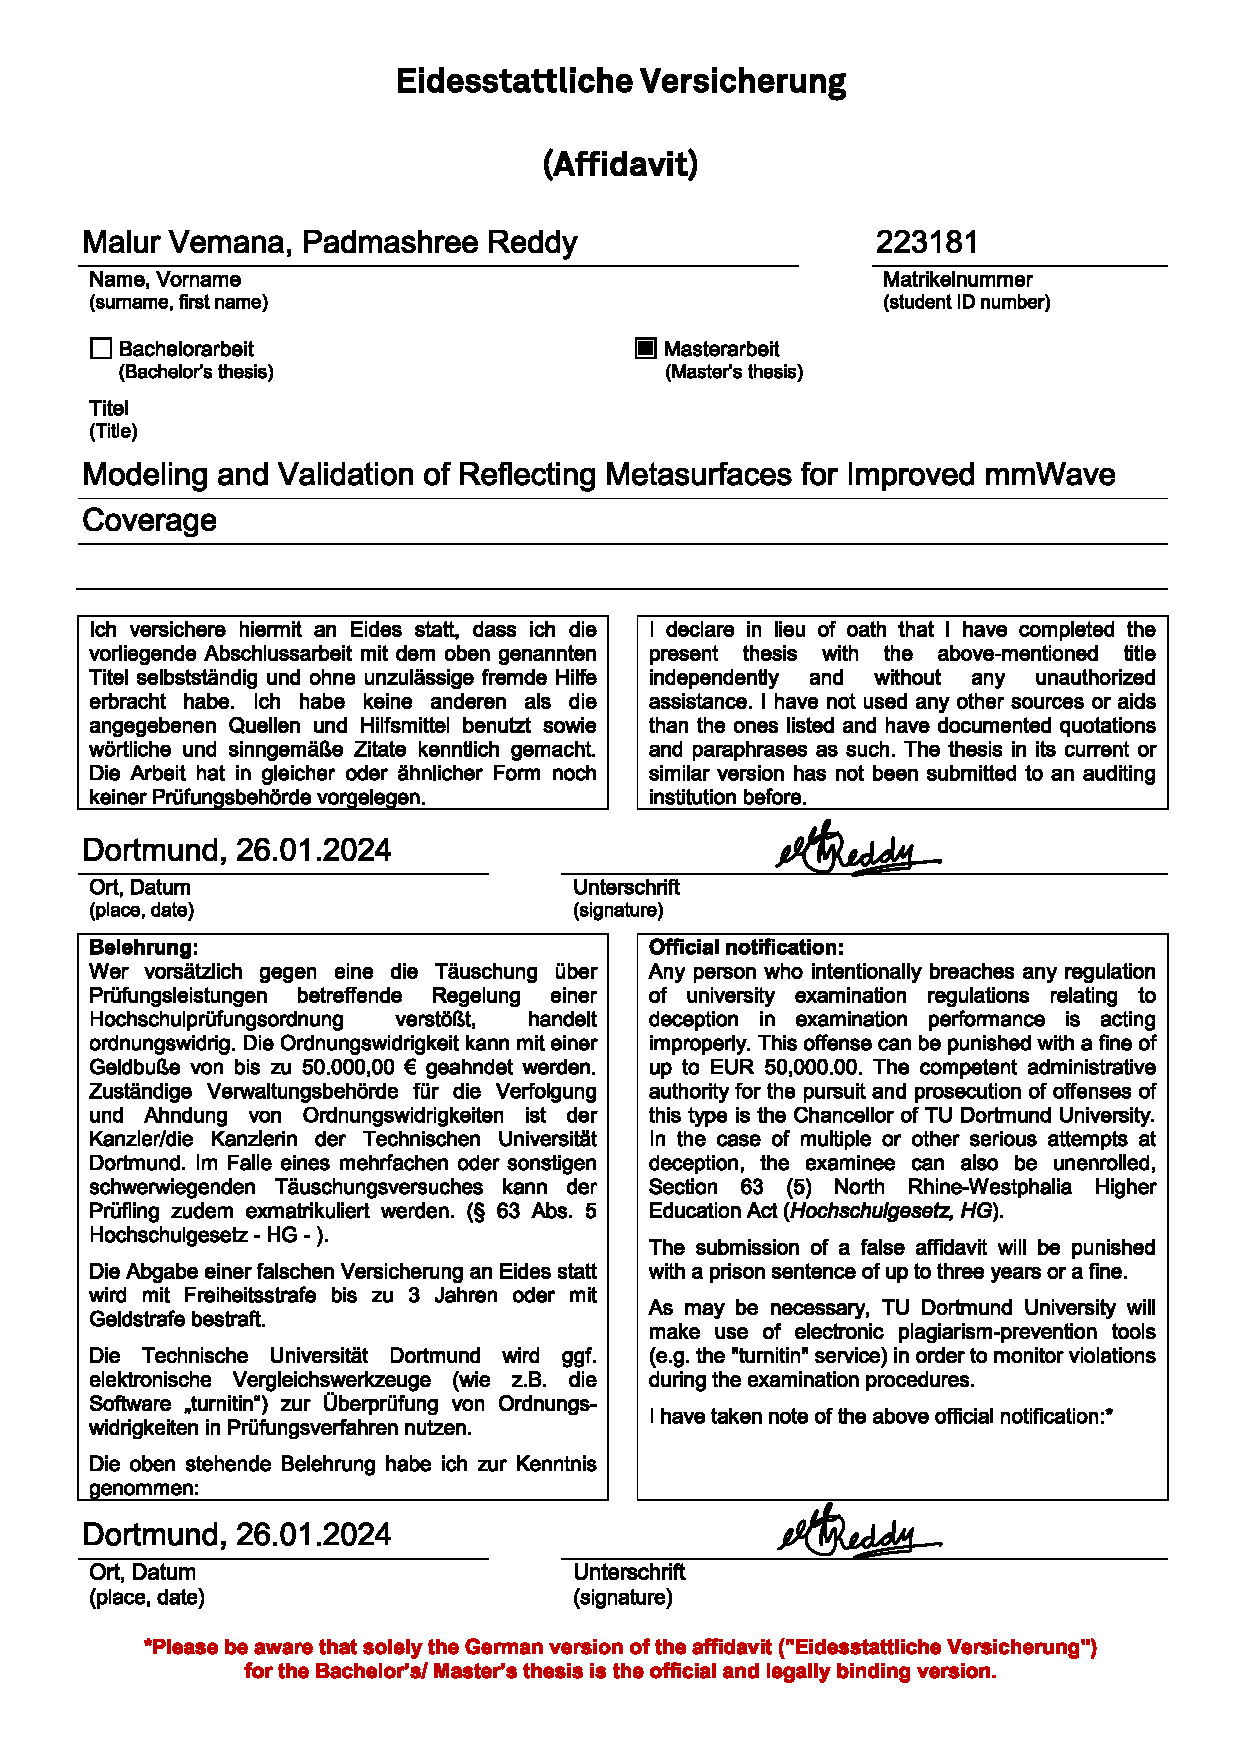
\includepdf[pages=-]{Eidesstattliche_Versicherung.pdf}
				\cleardoubleplainpage
				\chapter*{Abstract}
\label{abstract}
\addcontentsline{toc}{chapter}{\textbf{Abstract}}

This thesis delves into the dynamic landscape of \ac{mmWave} communication technology where the main focus is on conquering the challenges posed by increased path loss at \ac{mmWave} frequencies, particularly due to obstructions. Moving towards 6G, the resulting shadow regions need to be illuminated to make \ac{mmWave} networks investments feasible, where metasurface based \ac{SRE}s offer a pivotal solution by deliberately reflecting \ac{EM} waves to enhance performance. Addressing limitations of \ac{IRS}, such as complex deployment logistics and active power requirements, have prompted a shift towards passive reflectors such as \ac{HELIOS}. This thesis aims to solve the lack of channel models for \ac{HELIOS} reflectors by leveraging it as an efficient and scalable alternative, thus, offering a promising solution for future cellular networks. The thesis also highlights the potential advantages of HELIOS reflectors over \ac{IRS} in terms of peak gain and beamwidth and emphasizes the need for optimizing the performance.

The thesis then proceeds to develop an analytical model for the bistatic \ac{RCS} for the HELIOS reflectors and validate it by comparing with EM simulations. The thesis further highlights the main reflection lobes are well-represented, e.g., in regards to gain and beamwidth and also highlights the attained speed-up and the significant reduction in computing time of using the proposed model. Further focusing on implementing the analytical model in an urban scenario to predict the connectivity and improve the initial reflector geometry and position to optimize the \ac{mmWave} communication. The result shows the better coverage and stronger signals by IRSs than HELIOS reflectors due to its dynamic nature which allows it to focus on each UE position individually. Further investigation reveals that by fixing the node for IRS, an equivalent coverage to that of \ac{HELIOS} reflectors is achieved, thereby proving its applicability in sophisticated hybrid network planning and \ac{HELIOS} customization process.

\textbf{Keywords:}
\begin{itemize}
	\item Metasurface-aided mmWave communications
	\item Simulation and modeling of HELIOS reflectors
	\item Channel and reflection modeling
\end{itemize} 
				\cleardoubleemptypage     
				\setcounter{tocdepth}{2}
				\setcounter{secnumdepth}{2}
				
				\begin{spacing}{1.0}          % Verzeichnisse werden mit einzeiligem Abstand gesetz
					%\listoftodos % todo liste anzeigen
					
					%verzeichnisse drucken
					\tableofcontents             % Inhaltsverzeichnis
				\end{spacing}
				
				%%hauptteil
				\cleardoubleplainpage         % Das erste Kapitel des Hauptteils auf einer rechten Seite beginnen
				\mainmatter                   % die eigentliche Arbeit beginnen
				
				%\include{tex/example} % remobe this part at some point (add '%' at row beginning)!
				
				\chapter{Introduction}
In the never-ending quest of advancing wireless communication technology, the use of \ac{mmWave} frequencies has begun with 5G, thus offering future-proof data rates and network capacity due to the large available bandwidth \cite{Intro1, ericsson6g, nokia6g}. However, path loss at \ac{mmWave} frequency is much higher, particularly due to reduced object penetration, thus greatly reducing the effective cell and causing shadowing within \cite{6GWireless, 8373698}. 

Looking toward the future 6G, this shall be addressed by new concepts such as \ac{SRE}s \cite{CNI}. There, metasurfaces shall be used to improve connectivity, among other things, by using their capability to deliberately modify the reflection behavior of an impinging incident wave. There are two kinds of metasurfaces: \ac{IRS} and passive reflectors.
\begin{figure}[H]
	\centering
	\subfloat[mmWave communication in a nutshell with RX1 in LOS has well connectivity, and RX2 in NLOS condition has a poor connection.]{
		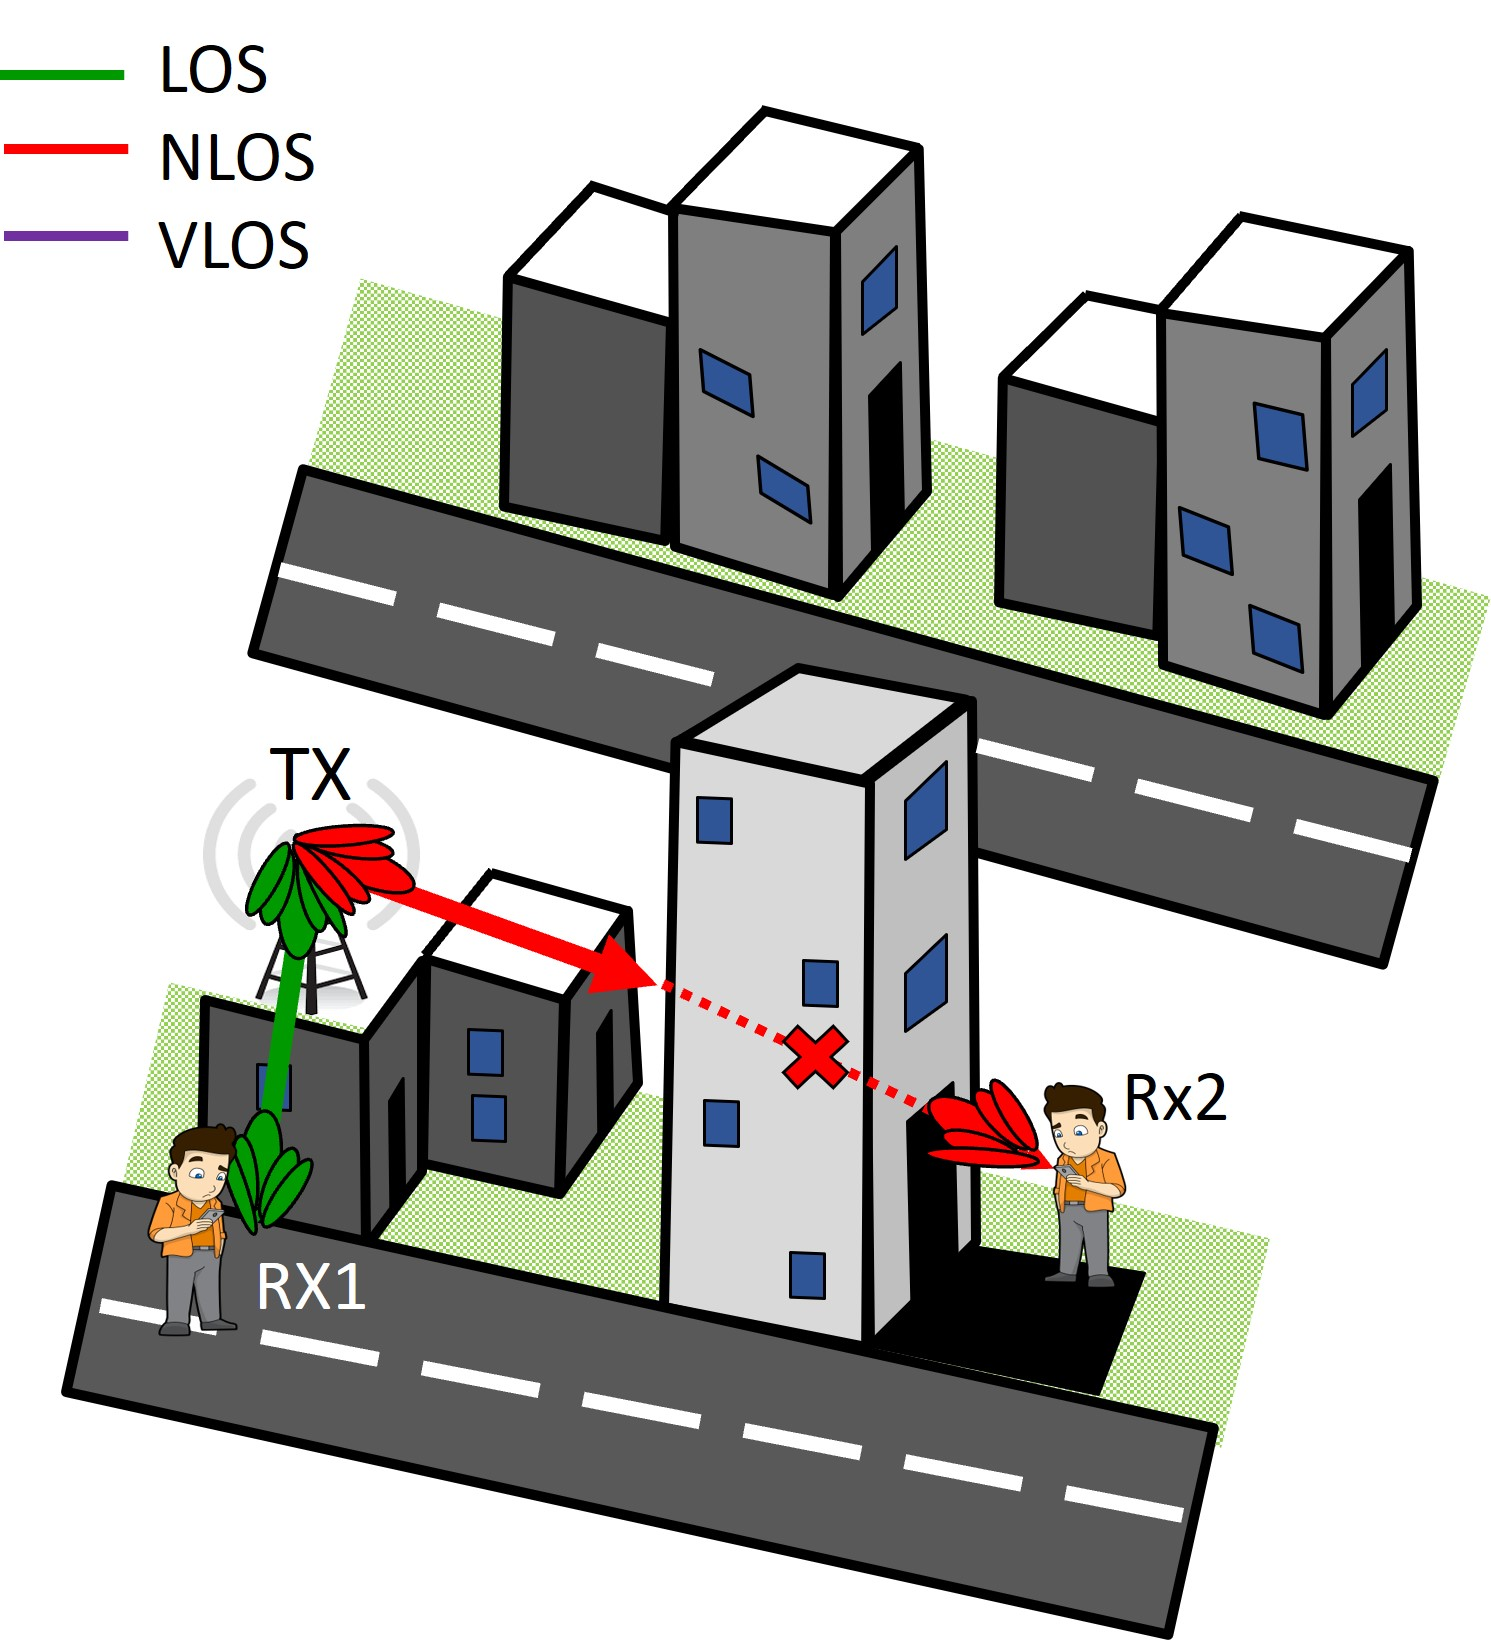
\includegraphics[width=0.45\linewidth]{images/Section 1 Images/Tx_Rx}
		\label{fig:Tx_Rx}
	}
	\hfill
	\subfloat[Future metasurface-enhanced mmWave networks can provide good connectivity in the NLOS regions by illuminating shadow regions using smart reflection behavior.]{
		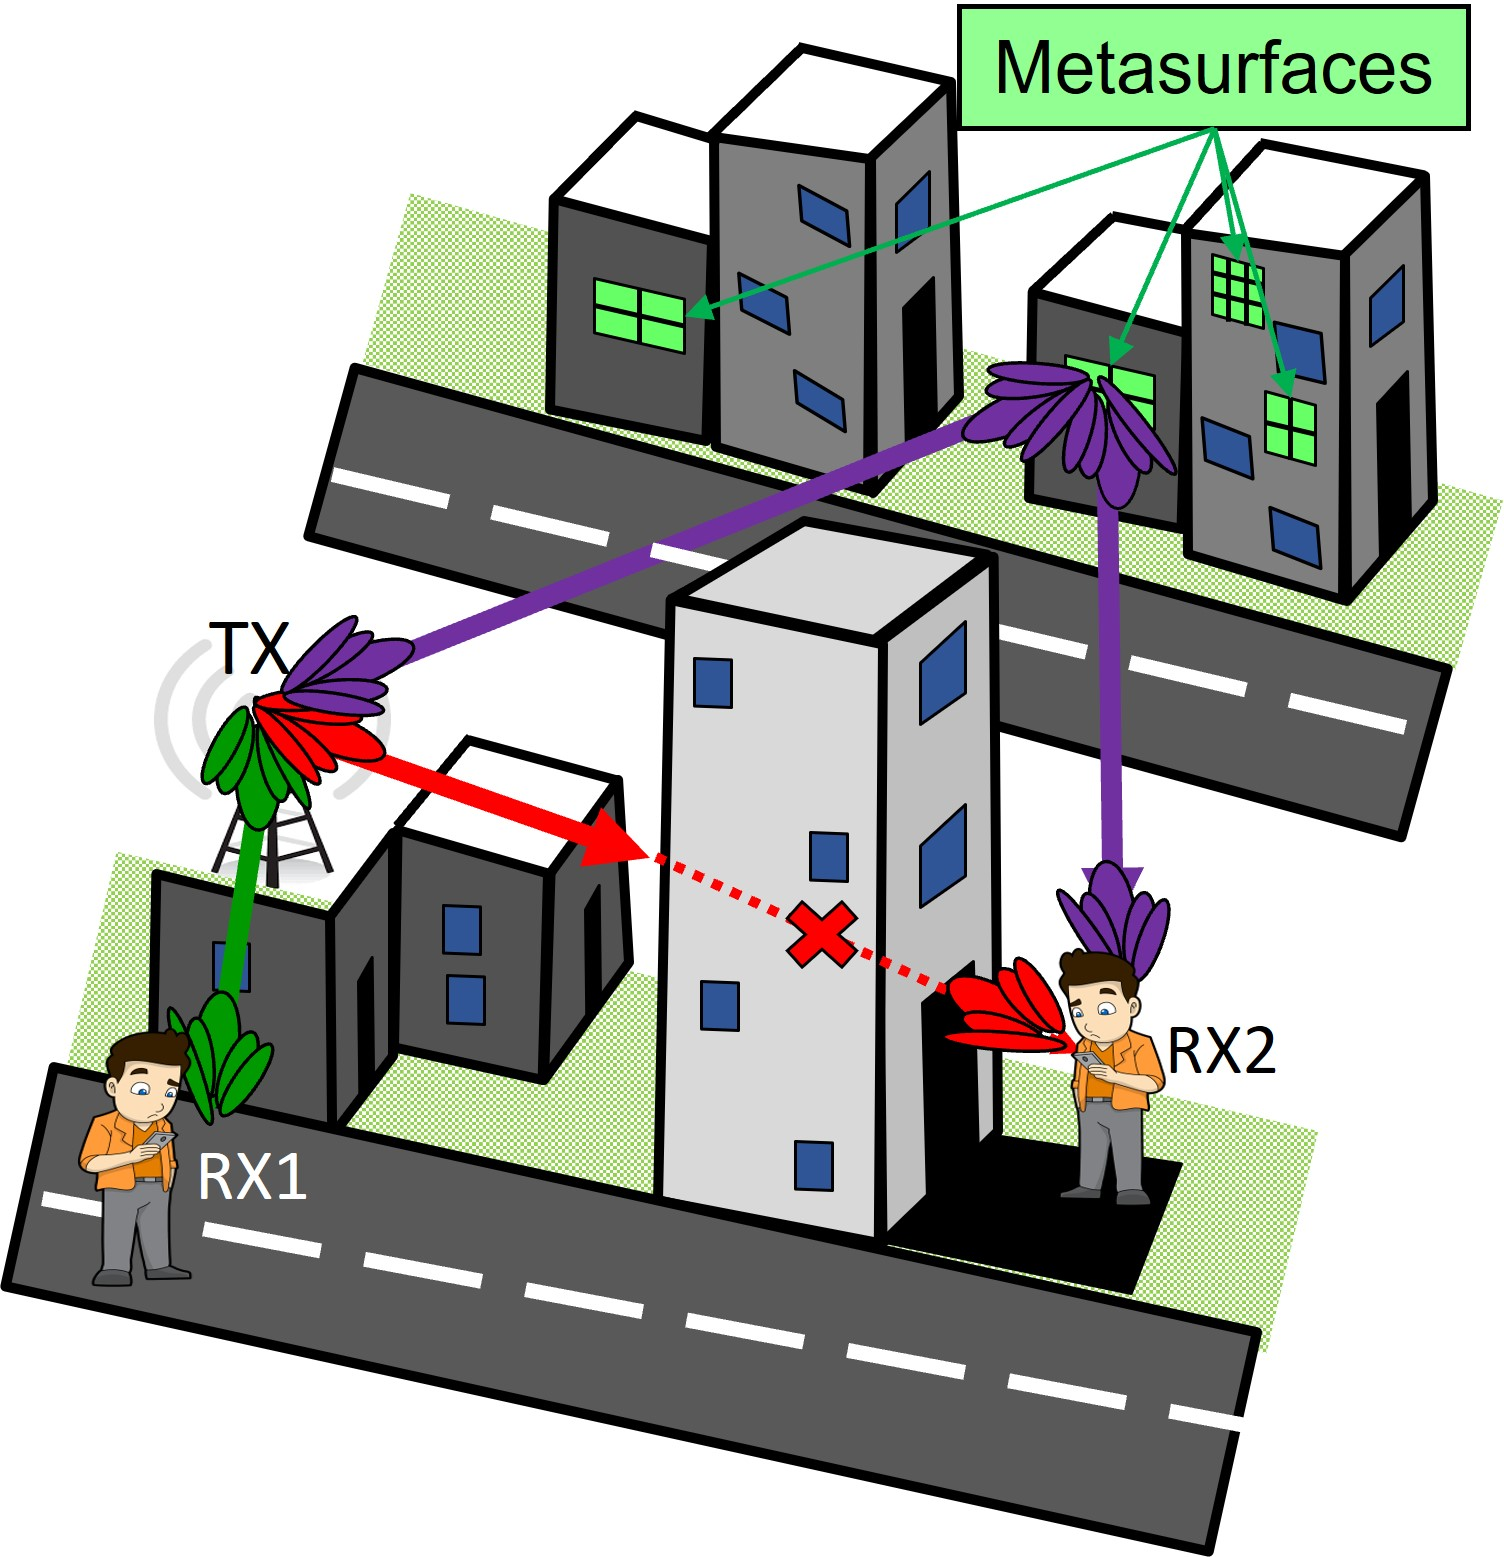
\includegraphics[width=0.45\linewidth]{images/Section 1 Images/Tx-Rx_Meta}
		\label{fig:Tx-Rx_Meta}
	}
	\caption[mmWave communication links from the transmitter (TX) to two differently positioned receivers (RXs): (a) RX1 in \ac{LOS} has a good connection, whereas RX2 in \ac{NLOS} cannot connect to the network. In (b) we illustrate how a metasurface that is mounted in the vicinity of the transceivers provides \ac{VLOS} connectivity to the \ac{NLOS} RX.]{mmWave communication links from the transmitter (TX) to two differently positioned receivers (RXs): (a) RX1 in \ac{LOS} has a good connection, whereas RX2 in \ac{NLOS} cannot connect to the network. In (b) we illustrate how a metasurface that is mounted in the vicinity of the transceivers provides \ac{VLOS} connectivity to the \ac{NLOS} RX.}
	\label{fig:Tx_RX}
\end{figure}
\ac{IRS} is a current hot topic in 6G research, primarily explored for its high flexibility by allowing dynamic control of reflected electromagnetic waves \cite{IRSdesignandapp, Shen2020ModelingAA, wu2019towards}. However, there are drawbacks to high energy consumption and active electronic components' complexity associated with \ac{IRS}. These challenges are not expected for the passive reflectors such as \ac{HELIOS} \cite{Helios}, making them the primary focus of this work.

In contrast to relying merely on simulations like current work, developing a HELIOS channel model or reflection model becomes critical since it provides a systematic analytical framework based on \ac{RCS} concepts \cite{Balanis, Kerr1989PropagationOS}. While simulation-based methods provide useful insights, an analytical model not only speeds up the computation, but it also enables a more rapid design and evaluation of passive reflector applications in urban communication networks. To demonstrate this practicality, we conduct a detailed analytical case study using HELIOS reflectors and compare them to \ac{IRS}s.

The remainder of this thesis is structured as follows. Sec. 2 of this master thesis introduces 5G mmWave communication before diving into the 6G metasurface concepts. Particularly, we introduce selected \ac{IRS} channel models and point out the lack of such for the recently proposed \ac{HELIOS} reflectors. Sec. 3 derives the analytical model of the bistatic RCS of \ac{HELIOS} reflectors and compares the arising reflection patterns to EM simulations. Sec. 4 assess the computing times before exploring our model in the context of an urban network scenario. There, we use it to optimize the connectivity and, at last, we directly compare \ac{IRS} and \ac{HELIOS} performance. Sec. 5 concludes this work by summarizing the key contributions and a brief outlook on future research.
%In the never-ending quest of wireless communication technology advancement, millimeter-wave (mmWave) frequencies have emerged, offering data speeds and network capacity. The basic qualities of mmWave, i.e., shorter wavelengths, make it a great choice for meeting the ever-increasing need for high-speed and high-capacity networks \cite{Intro1, ericsson6g, nokia6g}. However, the incorporation of mmWave into communication networks introduces high path loss due to obstructions, including greater atmospheric absorption and lower coverage \cite{6GWireless, 8373698}. As we look to the future, the transition to 6G seems inevitable. Beyond the capabilities of mmWave, 6G adds new concepts such as Smart Radio Environments (SREs) to improve network performance \cite{CNI}. SREs use intelligent components, in recent years, research into metasurfaces has received a lot of interest in the fields of wireless communications and radar technology. Metasurfaces, known for their capacity to precisely modify electromagnetic waves, have emerged as critical components in signal propagation. The two kinds of metasurfaces: Reconfigurable Intelligent Surfaces (RIS) and passive reflectors, interests us. Notably, the emphasis has switched from active to passive reflectors, representing a paradigm shift in research and development. These passive reflectors use the notion of altering signal reflections to improve coverage, and increase network efficiency by taking advantage of metasurfaces' natural benefits while reducing complexity and energy usage \cite{en14248219, LiSinghSievenpiper, FangLiChenSunXiaoHeZhou}.\\
%In light of this paradigm change, this thesis digs into the complexities of passive reflectors, proposing a complete methodology to optimize and expedite the use of these reflecting surfaces while also shining light on its distinguishing features and usefulness in modern communication systems. Unlike most simulation-based techniques, our work presents an analytical model based on Radar Cross-Section (RCS) principles that aims to speed up computations without sacrificing precision, opening the path for real-time applications in urban communication networks.\\

%We deploy the passive reflector in a simulated urban situation to validate our analytical model in practice \cite{Helios}. This implementation is intended to evaluate the analytical model's performance and efficacy in a dynamic and difficult context. In this thesis work, we go deeper into the theoretical underpinnings, design principles, and empirical validations, providing a holistic examination of passive reflectors' revolutionary potential in the mmWave and 6G landscapes.\\
%\Cref{fig:Tx_Rx} displays a standard communication scenario similar to a typical 5G network with transmitter (Tx) and two receivers (Rx1 and Rx2) where Rx1 has a Line-of-Sight (LOS) path and Rx2 encounters a Non-Line-of-Sight (NLOS) path to the Tx, resulting in path losses designated as $PL_{Tx. Rx1}$, and $PL_{Tx. Rx2}$, respectively, in \si{\decibel}.
%\Cref{fig:Tx-Rx_Meta} depicts a transformational perspective in the context of 6G communication, proposing a metasurface to handle NLOS circumstances. Notably, when there is an NLOS path between Tx and Rx2, a virtual LOS connection is constructed by including a metasurface mounted on the building. $PL_1$, and $PL_2$ indicate the path losses associated here as depicted. Unlike classic NLOS scenarios, the metasurface presents a unique signal attenuation mitigation technique, which has the potential to improve communication reliability and performance.\\
%\Cref{cha:Background} of our thesis begins by explaining the motives for harnessing mmWave communication and investigating solutions such as SREs and metasurfaces. We introduce known IRS models and compare them with the novel notion of HELIOS passive reflectors. \Cref{Simulation and Analytical Modeling of HELIOS Reflectors} focuses on the derivation of our analytical model for the HELIOS model's reflection pattern, using bistatic RCS principles and comparing the findings to EM simulations. In \Cref{Performance Evaluation and Case Study}, we undertake a complete performance evaluation, comparing our analytical model's computational time to EM simulations. Expanding our analysis, we build an urban environment, anticipate communication channel models, and aim to optimize the model by changing the geometry and reflector position. \Cref{Conclusion} concludes this work by summarizing our accomplishments and laying the groundwork for future research by identifying potential areas for investigation and improvement.
    % einführung
			%	\chapter{Background}
\label{cha:Background}
				\chapter{Background} \label{cha:Background}
This section contains the technical background for this thesis where we first introduce \ac{mmWave} specific cellular communications technology aspects in \Cref{Millimeter wave communication}. In \Cref{Channel Modeling}, the focus is on channel modeling, highlighting the differences between \ac{LOS} and \ac{NLOS} conditions. \Cref{Metasurfaces} provides a comprehensive introduction to the technology concept of metasurfaces that are envisioned to be active components of future sixth-generation (6G) radio access networks, but passive variants may already be employed in conjunction with fifth-generation (5G) networks. We then introduce existing \ac{IRS} channel models that are taken into consideration for further reinterpretation. Lastly, based on previously presented related works, \Cref{Related Work or Scope of Thesis} formulates the aims of this master thesis.
\section{Millimeter Wave Communication} \label{Millimeter wave communication}
Globally, the demand for 5G networks is rising quickly. The wireless communication of upcoming generations needs to be improved to meet our constantly increasing demand for faster data speeds and lower latency. Applications such as the \ac{IoT}, augmented reality, and driverless vehicles necessitate higher performance networks to function successfully and deliver a smooth user experience \cite{BANAFAA2023245, Towards6G}. To keep up with these growing requirements and ensure that wireless networks can meet future demands, new technology is required. The much-needed scalable increases in network capacity and peak data rates can be achieved using \ac{mmWave} communication technology. Due to more hostile propagation characteristics in terms of higher atmospheric absorption and increased susceptibility to obstacles and environmental conditions, the move to directional communications necessitates for compensating the additional path loss. Due to this, cellular mmWave communications will be drastically different from those of the current typically sub-6 GHz networks. These variations make it harder to use \ac{mmWave} communications to their fullest potential, as discussed in this section.

In typical commercial mobile wireless telecommunication systems, wireless and mobile systems operate in a specific frequency band within the sub-\SI{6}{\giga\hertz} spectrum. However, these frequency bands are saturated as a result of the exponential growth in network data traffic in current wireless communication. According to recent studies by \cite{diakhate2019propagation}, the bandwidth currently present in the sub-\SI{6}{\giga\hertz} spectrum, which is covered by 5G \ac{FR1}, will not be sufficient to achieve the capacity required for the upcoming systems.
\begin{figure}[H]
	\centering
	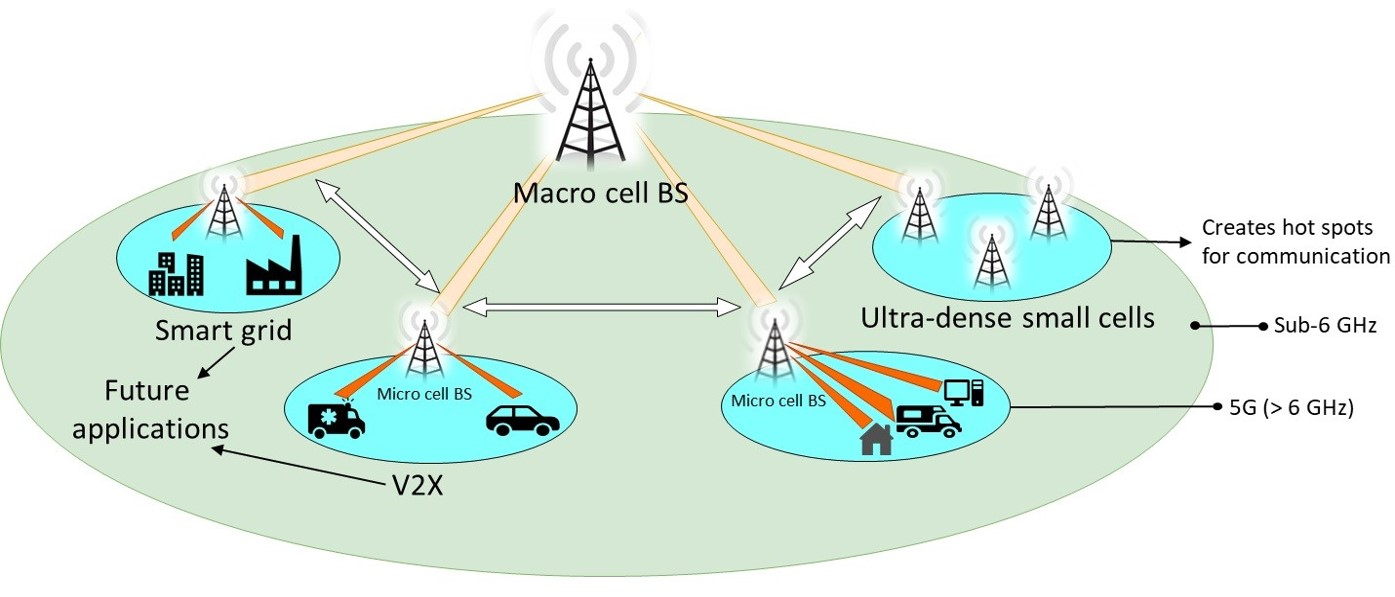
\includegraphics[width=1.0\linewidth]{images/Section 2 Images/5Gmm}
	\caption{Illustration of typical deployment of mmWave communications with use cases and future applications with the communication established between macrocell base stations at sub-\SI{6}{\giga\hertz} to the microcell base stations \cite{mmWavefig1, Sakaguchi2017WhereWA}.}
	\label{fig:5gmm}
\end{figure}
The \ac{mmWave} frequency band, which offers greater frequency bandwidths, enters the picture at this point. The \ac{3GPP} supports an additional frequency range with 5G, so-called \ac{FR2} that includes seven operational bands between \SI{24.2}{\giga\hertz} and \SI{71}{\giga\hertz}, namely n\num{257}, n\num{258}, n\num{259}, n\num{260}, n\num{261}, n\num{262}, and, n\num{263} \cite{3GPP17}. However, not all frequencies are included because, depending on the nation, only the ranges between \num{24.25}-\SI{29.5}{\giga\hertz}, \num{37}-\SI{43.5}{\giga\hertz}, \num{47.2}-\SI{48.2}{\giga\hertz}, and \num{57}-\SI{71}{\giga\hertz} shall be used.More frequency ranges have recently been identified for 6G \cite{3GPP17}, including \ac{FR4} which covers the frequency range of \SI{71}{\giga\hertz} to \SI{114.2}{\giga\hertz} and is anticipated to be used for autonomous and connected vehicles under the umbrella of \ac{ITS}. The \ac{FR5} category includes frequencies above \SI{114.2}{\giga\hertz}. Additionally, \ac{FR3} covers the majority of the space between \ac{FR1} and \ac{FR2}, i.e., the "No Man's Land" \cite{Qualcomm} between \SI{10}{\giga\hertz} to \SI{20}{\giga\hertz}. As a result, with FRs \num{2}–\num{5}, it is possible to see how crucial the spectrum above \SI{6}{\giga\hertz} will be for future communication networks.

\Cref{fig:5gmm} depicts a typical mmWave communication deployment with several use cases. We see communication linkages formed in both the sub-\SI{6}{\giga\hertz} and greater than \SI{6}{\giga\hertz} frequency ranges in this illustration. The deployment also includes ultra-dense tiny cells specifically placed to generate communication hotspots. In terms of future applications, the figure suggests smart grid and V2X (Vehicle-to-Everything) connectivity. These developing application cases demonstrate mmWave technology's adaptability and disruptive promise in enabling not only better mobile broadband but also critical infrastructure and intelligent transportation systems.

The \ac{mmWave} spectrum is expected to be used by future mobile radio networks to deliver higher data rates for novel use cases like \ac{XR}. Virtual reality, autonomous vehicles, swift factory robots, and 8K video streaming are some additional cutting-edge services made possible by \ac{mmWave} technology.
\subsection{Propagation Characteristics of mmWave} \label{Characteristics of 5G mmWave}
The \ac{EM} waves with a wavelength $\lambda$ of \SI{1}{\milli\meter} to \SI{10}{\milli\meter} are known as \ac{mmWave}. Using the formula $\ f = \frac{c}{\lambda}$, where $c$ is the speed of light $ (\approx \num{3} \cdot \SI{e8}{\meter}/\si{\second})$, we convert the wavelength to obtain a frequency range of \SI{30}{\giga\hertz} to \SI{300}{\giga\hertz}. \ac{mmWave} is also referred to as the \ac{EHF} band or the \ac{UHF} band, according to the \ac{ITU} \cite{ITU_EHF}. From an industry perspective, frequencies above \SI{20}{\giga\hertz}, sometimes even from above \SI{10}{\giga\hertz}, are also referred to as \ac{mmWave}.

So far, we have emphasized the advantages of \ac{mmWave} technology, namely that it allows for high network capacity that is future-proof and peak user data rates because of the wide available bandwidth. However, there are also drawbacks to using \ac{mmWave} frequencies. Before the adoption of 5G, frequency bands above \SI{6}{\giga\hertz} were thought to be unsuitable for mobile wireless communications due to their susceptibility to high path losses, especially as a result of obstruction by any objects, including buildings, people, and vegetation \cite{6GWireless}. At various frequencies and distances, the path loss calculations show how frequency affects wireless communication. The path loss is roughly \SI{92.4}{\decibel} at a frequency of \SI{2}{\giga\hertz} and a distance of \SI{100}{\meter}. In contrast, the path loss dramatically rises to almost \SI{108.5}{\decibel} at a higher frequency of \SI{28}{\giga\hertz}. This represents a large difference of roughly \SI{16.1}{\decibel}. When comparing a concrete wall to a similar wall at lower frequencies, the penetration loss at \SI{28}{\giga\hertz} through the wall may be much larger, up to about \SI{30}{\decibel}. Furthermore, compared to absorption losses at lower frequencies, the human body is predicted to experience a greater path loss at \SI{28}{\giga\hertz}, possibly approaching \SI{20}{\decibel}.

Environmental factors include increased atmospheric absorption, a greater impact by rain and snow, increased penetration losses, and, increased diffuse scattering due to surface roughness becoming relatively large compared to the wavelength \cite{6GWireless}. While these obstacles restrict the use of \ac{mmWave}, improved antenna technology has been suggested to make up for the extra losses with the idea of grouping numerous, now smaller, antennas into arrays that are then used for beamforming.
\subsection{Beamforming and Beam Management} \label{Beam Steering and Management}
As \ac{mmWave} has short wavelengths and high frequencies, antennas get smaller and can be combined into antenna arrays with a small form factor. Through the use of beamforming and such antenna arrays, the antenna directivity is made possible in a specific direction. This will be used for transmission and reception. There, the impact of significant path loss can be lessened or even mitigated by the beamforming gain. The formed beam can be configured in any way, but the idea is to direct the resulting antenna beam along the strongest propagation path for maximum efficiency. In addition, the antenna pattern can have some directions nulled to lessen interference from/at other devices. A multi-armed antenna beam may also be realized to serve multiple users, depending on the hardware architecture. When two or more antenna elements are arranged spatially and electrically in arrays that are connected, directional radiation patterns can be created. The feed network, which refers to the connections between the RF front end and the antenna elements, creates a phased array by assigning each element a phase. To improve the received signals, adjustments may even be made to the amplitude of the individual antenna branches \cite{Ali2017BeamformingTF}. The individual antenna elements' radiation patterns, mounting orientations, and polarizations as well as the geometry of the array all have an impact on how well the array works.

Because wireless communication frequently serves mobile users, the beam directions must be continuously aligned. Beam management processes include beam tracking and beam switching techniques for sustaining the established link. With slight adjustments, the former constantly modifies the Tx and Rx beam orientation. This dynamic alignment is critical for overcoming the hurdles given by mobile users' changing position, and maintaining a stable and high-quality connection. Beam tracking allows the system to monitor the user's location and modify the beam direction in real time to maintain the best possible link. Beam-switching techniques, in addition to beam tracking, play an important part in seamless communication by permitting smooth transitions between available propagation paths and base stations when the user's movement necessitates such handovers \cite{s23094359, 8947954}. These beam management approaches are critical for delivering the performance and dependability that current wireless communication systems demand.
\section{Channel Modeling } \label{Channel Modeling}
Channel modeling is an essential part of the design of efficient wireless communication systems. To design a communication system that performs reliably and effectively, we need a process to characterize and optimize its behavior based on its fundamental mathematical representation of the physical channel \cite{Rappaport, rappaport2015millimeter}. Thus, the representation of how transmitted EM waves interact with the environment is one of the core values of channel modeling. The properties such as free-space path loss and interactions with objects in terms of reflection, diffraction, and scattering are modeled \cite{rappaport2015millimeter, electronics12092014}. Moreover, the antenna patterns of the transmitter and receiver are considered. These are quantifiable, making it possible to predict the channel conditions in particular environments. As we delve further into this subject, we investigate various channel modeling methodologies, approaches, and tools that are used to fully comprehend the \ac{mmWave} communication environment and its effect on system performance.

A Tx and Rx scenario is succinctly illustrated in \Cref{fig:TxRx}, which also shows the LOS path to the receiver at Rx1 with gain $G_{Rx1}$ and NLOS path to the receiver at Rx2 with gain $G_{Rx2}$ from the transmitter Tx with gain $G_{Tx}$. To enhance this illustration, a sample Channel Impulse Response (CIR) is shown on the right, providing a practical understanding of how the channel response could seem for both LOS and NLOS paths with some amount of propagation delay. The time-varying reaction of a communication channel to an impulse signal is represented by the channel impulse reaction, which effectively characterizes the features of the channel \cite{ITUReport}.

\begin{figure}[tb]
	\centering
	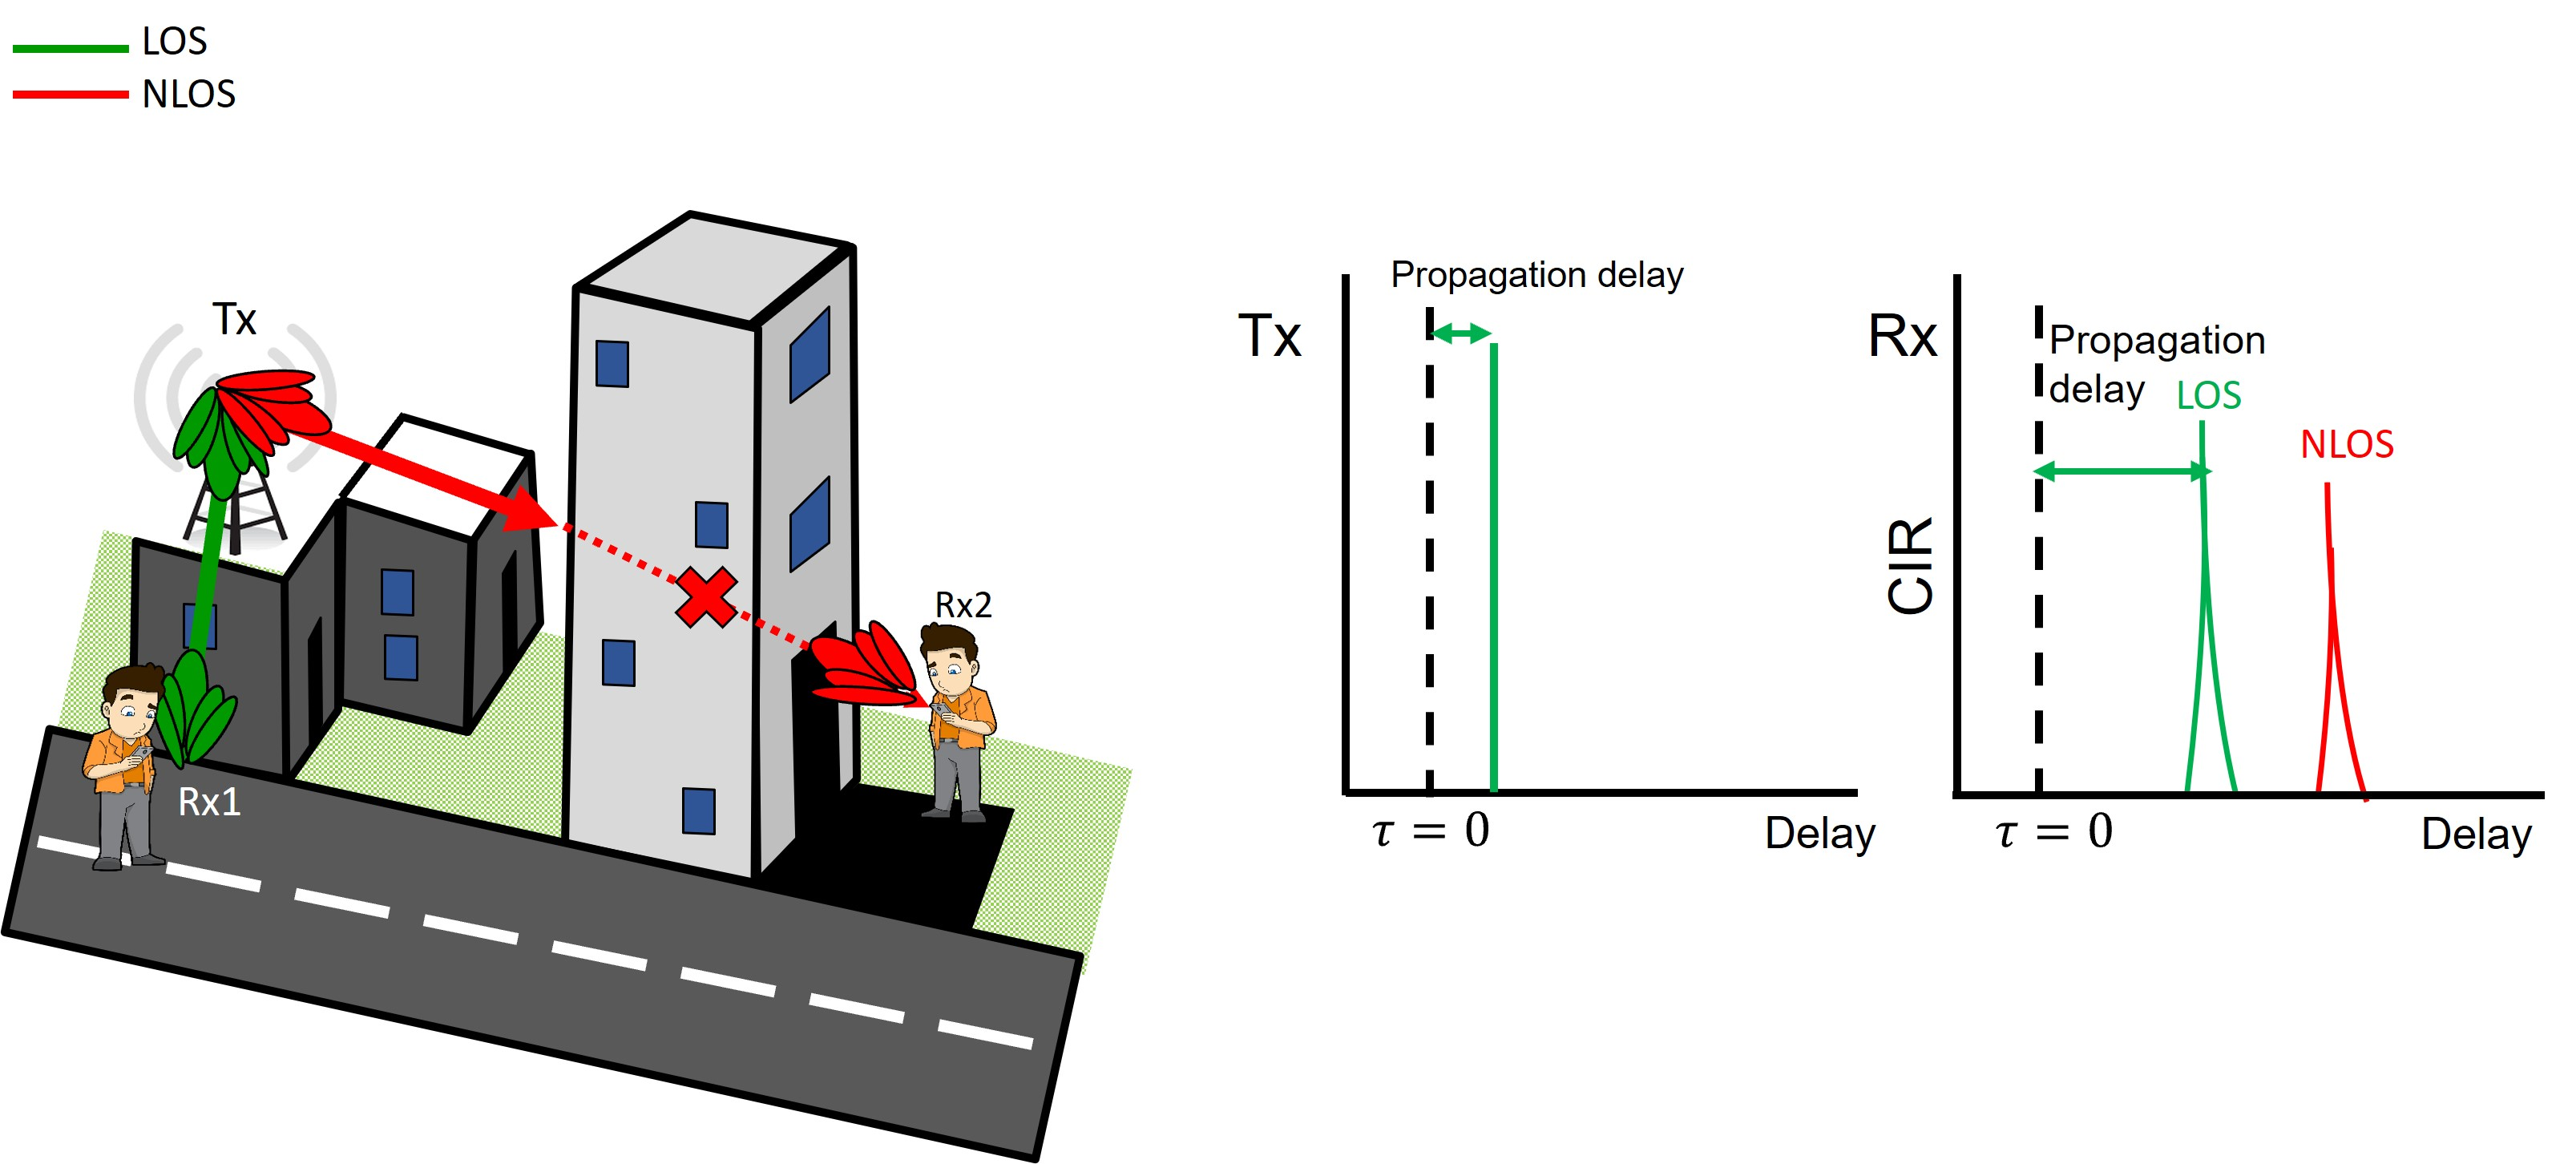
\includegraphics[width=1.0\linewidth]{images/Section 2 Images/TxRx}
	\caption{Illustration of a simple communication system with the transmitter Tx with gain $G_{Tx}$ in LOS path with Rx1 with gain $G_{Rx1}$ and NLOS path with Rx2 with gain $G_{Rx2}$. The sample CIR graphs on the right include both the LOS and NLOS paths for the general grasp of the idea \cite{ITUReport}.}
	\label{fig:TxRx}
\end{figure}
\subsection{Propagation Environment} \label{Propagation Environment}
Many different channel modeling techniques can be used in this setup for system and network planning \cite{KabulUni, 3GPP17}. Popular models include WINNER and COST, and as the world transitions to \ac{mmWave}s, models from the \ac{3GPP}, \ac{ITU}, and IEEE are becoming increasingly important. A brief overview of existing schemes is followed by a detailed introduction of a few channel models \cite{diakhate2019propagation}.

The suitability or applicability of channel models depends on those traits. Others are restricted to 2D propagation, while some cannot be used at \ac{mmWave}s because they only take into account sub-\SI{6}{\giga\hertz} frequencies. The computationally difficult and labor-intensive modeling alternative to any such method is ray-tracing which simulates the propagation of EM waves in a particular environment \cite{rappaport2015millimeter,sun2018propagation} by following rays from the transmitter to the receiver and accounting for reflections, diffraction, and scattering \cite{pen}. Stochastic modeling is a form of statistical modeling, that uses probability distributions to describe the channel properties based on measurements or ray-tracing simulations. With these types of models, whether \ac{LOS} or \ac{NLOS} conditions are present is frequently a crucial parameter for path loss prediction.

\Cref{Mmwave Channel modeling efforts by different organizations} provides an overview of such available mmWave channel models. A hybrid propagation model that combines the previously described deterministic and stochastic elements serves as the foundation for the few-channel model. The deterministic component uses ray-tracing to simulate the spread of radio waves by following each individual ray as it interacts with various elements of the environment. To take into account the randomness and variability in the propagation environment, the stochastic component is based on statistical models \cite{8207426}. Apart from these, 3GPP propagation models are empirical, i.e., they extract characteristics that describe radio wave propagation in various situations from real-world measurement data.
\begin{table}[tb] % H -> dieses objekt wird genau da wo der code steht festgenagelt
	\footnotesize
	\caption{\ac{mmWave} channel modeling efforts by different organizations with their operating frequencies and the kind of propagation models that they support.}
	\label{Mmwave Channel modeling efforts by different organizations}
	\centering
	\begin{tabular}{C{3.25cm}|C{1.3cm}|C{1.8cm}|C{0.7cm}|C{2.3cm}|C{1.7cm}|C{1.9cm}}
		\textbf{Channel Model} & \bf Source & \bf Frequency & \bf Year & \bf Environment & \bf Mobility Support & \bf Propagation Models \\
		\hline 
		\ac{5GCM} & \cite{5GCM, KabulUni} & \SI{28}{\giga\hertz}, \SI{38}{\giga\hertz}, \SI{73}{\giga\hertz} & \num{2011} & Indoor, outdoor & Yes & Hybrid\\
		\hline 
		\ac{METIS} &  \cite{METIS, KabulUni} & up to \SI{100}{\giga\hertz} &  \num{2012} & Indoor, outdoor & No & Hybrid \\
		\hline 
		Third Generation Partnership Project (\ac{3GPP}) & \cite{3GPP17, KabulUni} & up to \SI{100}{\giga\hertz} &  \num{2017} & Indoor, outdoor & Yes & Empirical\\
		\hline 
		\ac{MiWEBA} & \cite{miwebaquadriga, weiler2016quasi} & \SI{60}{\giga\hertz} &  \num{2014} & Outdoor & No & Stochastic \\
		\hline 
		\ac{QuaDRiGa} & \cite{miwebaquadriga} & \SI{30}{\giga\hertz} & \num{2014} & Indoor, outdoor & Yes & Hybrid \\
	\end{tabular}
\end{table}
Because these models are the result of intensive field testing and measurement, they are useful instruments for forecasting signal behavior and enhancing mobile communication system performance. In the following sections, we consider alternative channel models. The free-space path loss model is first introduced in \Cref{Free space propagation model} and then followed up by the 3GPP UMi and UMa models in \Cref{3GPP channel model}.
\subsection{Free-Space Propagation Model} \label{Free space propagation model}
The FSPL model constitutes the fundamental and most simplistic channel model considering a radio signal in free space, i.e., there is LOS between Tx and Rx and no multipath propagation. \Cref{Eq:Free space propagation} describes the received power in free-space conditions.
\begin{equation} \label{Eq:Free space propagation}
	P_{Rx}= P_{Tx} \frac{G_{Tx} \cdot G_{Rx} \cdot \lambda^2 }{(4 \cdot \pi \cdot r_{Tx, Rx})^2}
\end{equation}
Here $P_{Tx}$ and $P_{Rx}$ are the transmitted and received power in Watts, respectively, $r_{Tx, Rx}$ is the 3D \ac{LOS} distance between the transmitter and the receiver, $G_{Tx}$ and $G_{Rx}$ are the gains of the transmitter and receiver antennas relative to an isotropic radiator with a unit gain, and $\lambda$ is the wavelength of the carrier in \si{\meter} \cite{9205413}.

Accordingly, the power loss between $P_{Tx}$ and $P_{Rx}$ is referred to as propagation path loss $PL_{dB}$, as depicted in  \Cref{Eq:path loss formula}. Combining \Cref{Eq:Free space propagation} and \Cref{Eq:path loss formula}, and moving from linear to decibel presentation, we provide the logarithmic FSPL channel model in the FSPL in  \Cref{equation1}. \Cref{fig:fspl} depicts the relation between path loss in \si{\decibel} as a function of Tx-Rx distance $r_{Tx, Rx}$ in \si{\meter}. 
\begin{equation} \label{Eq:path loss formula}
	PL_{dB}= 10\cdot \log_{10} \left( \frac{P_{Tx}}{P_{Rx}} \right) 
\end{equation}
\begin{equation} \label{equation1}
	PL_{dB}= -147.5 \; \si{\decibel} + 20 \cdot  \log_{10} \left(\frac{r_{Tx, Rx}}{\SI{1000}{\meter}} \right) + 20 \cdot \log_{10} \left(\frac{f}{\SI{1000}{\mega\hertz}}\right) + G_{Tx, dB} + G_{Rx, dB}
\end{equation}
\begin{figure}[tb]
	\centering
	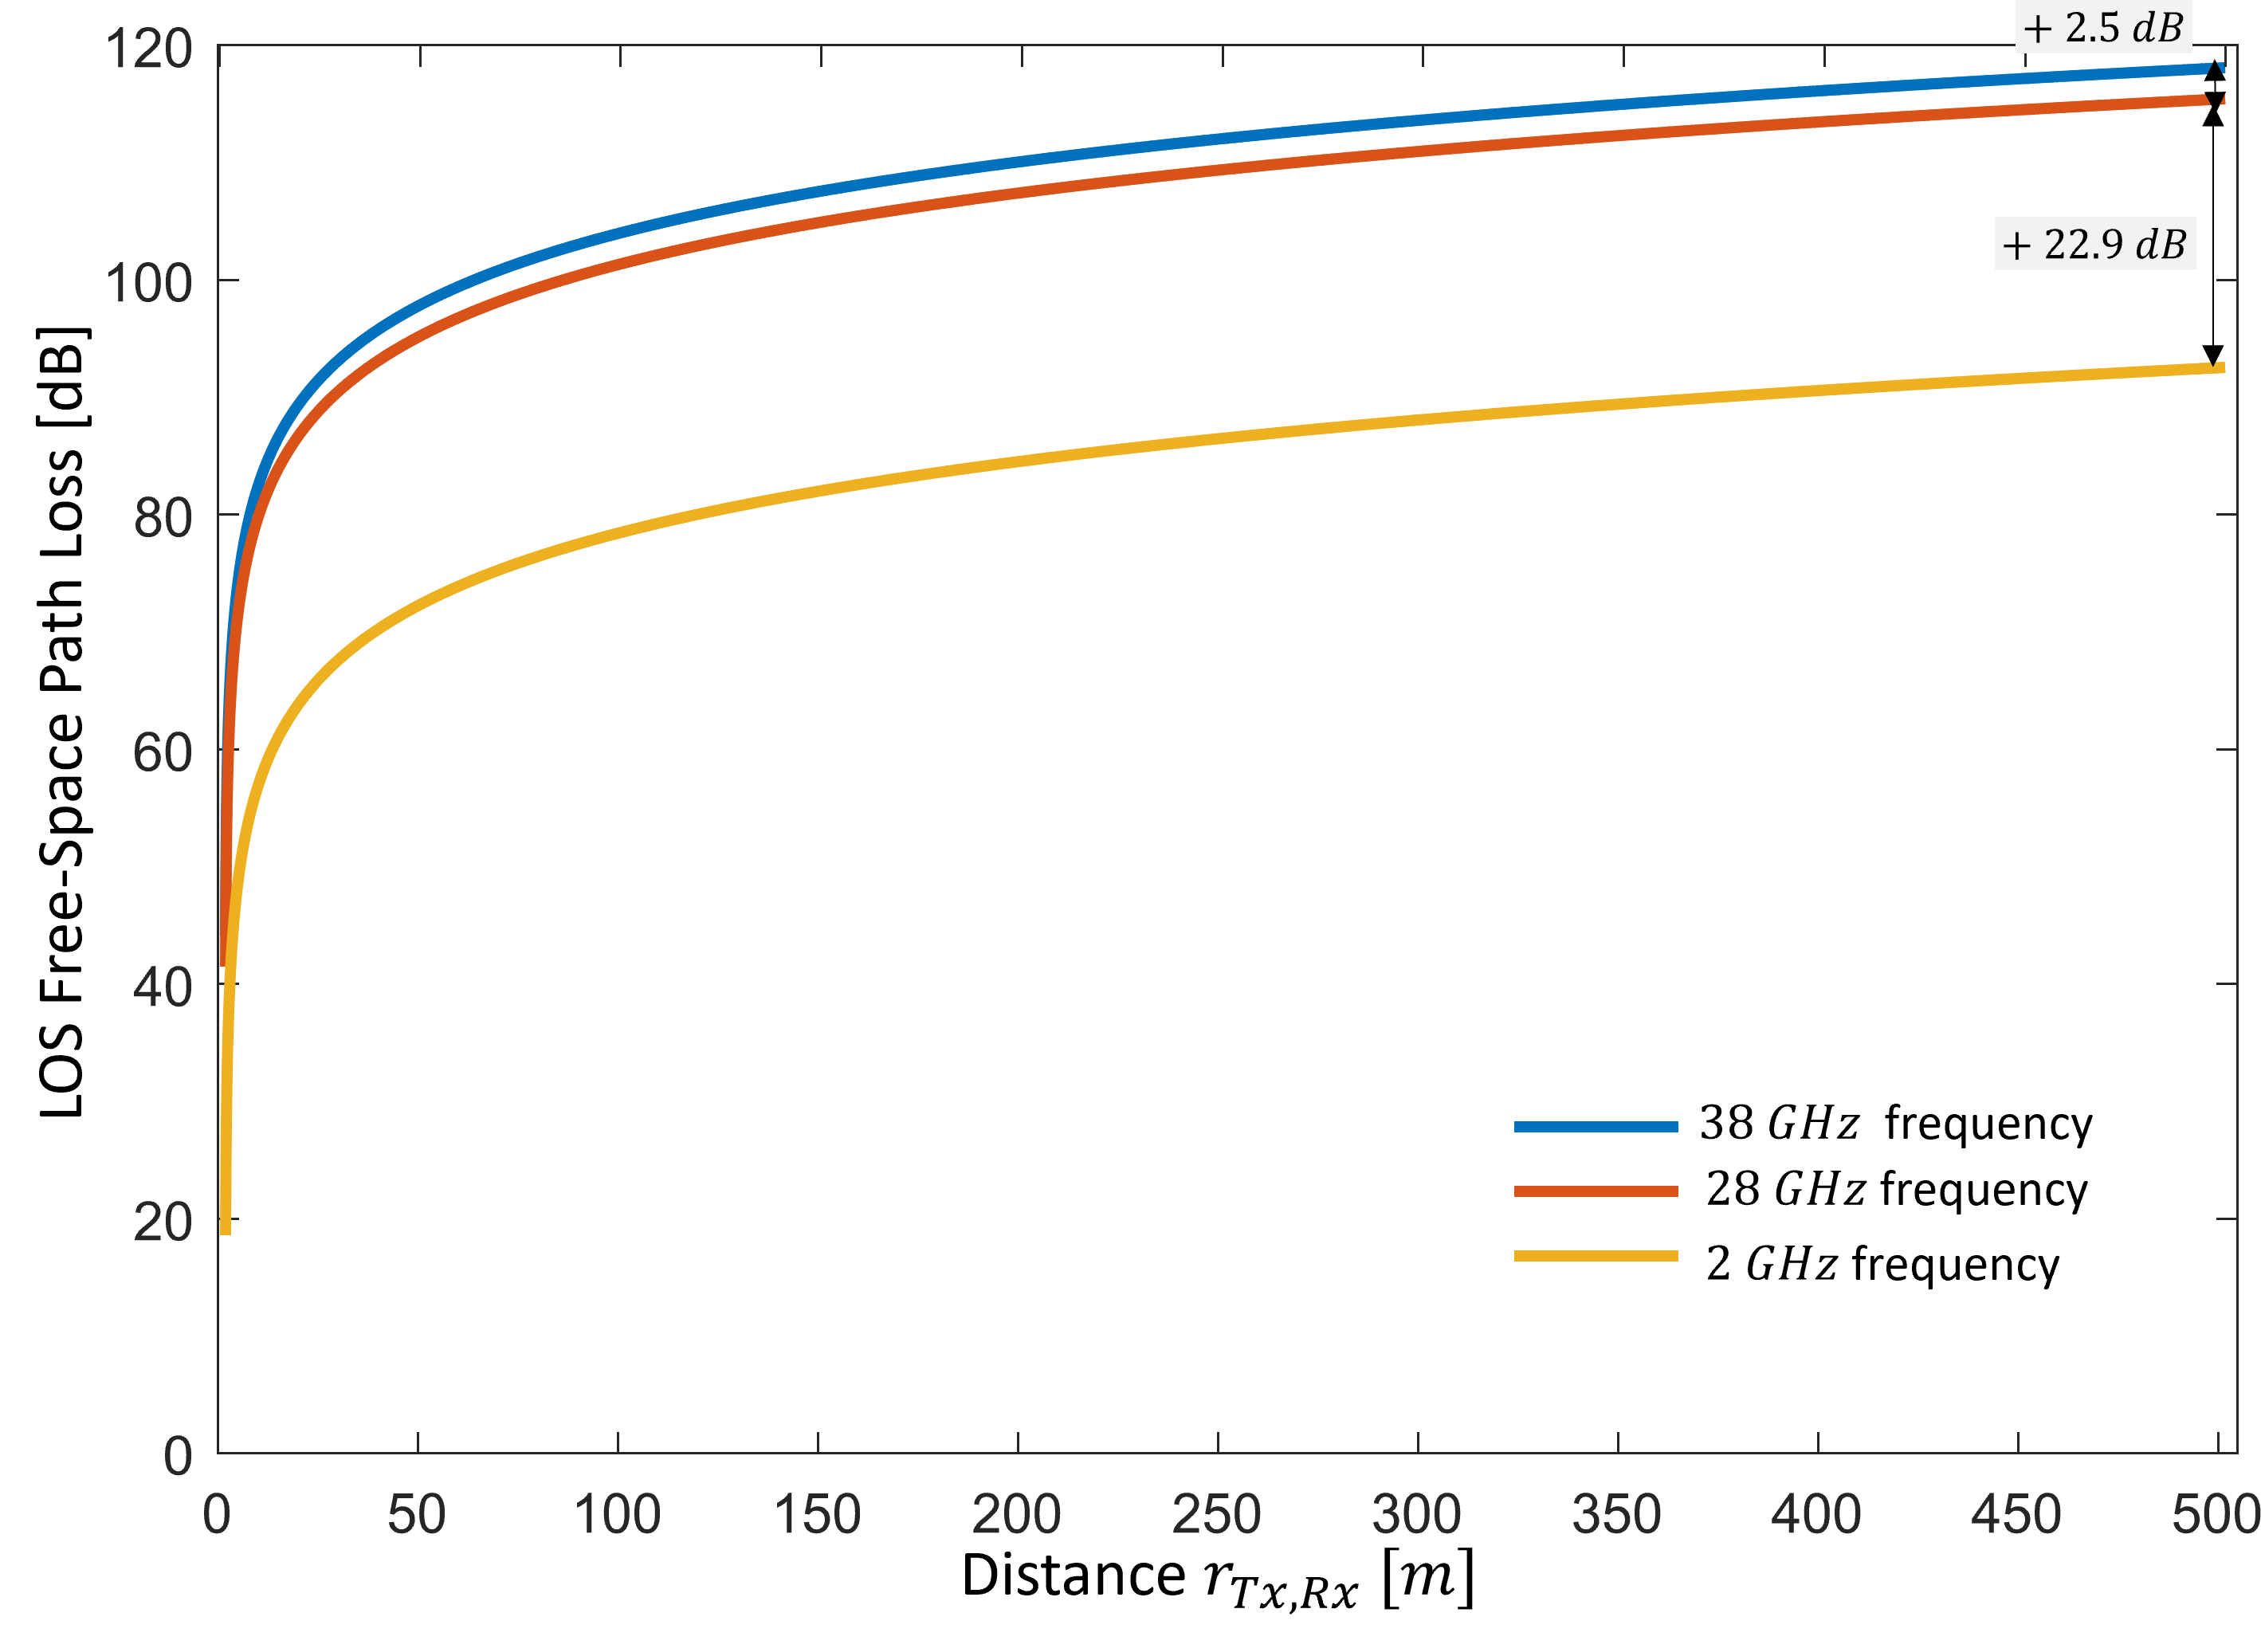
\includegraphics[width=0.8\linewidth]{images/Section 2 Images/fspl}
	\caption{Free-space path loss propagation in \si{\decibel} as a function of Tx-Rx distance in \si{\meter} for the \ac{LOS} condition at \SI{38}{\giga\hertz}, \SI{28}{\giga\hertz}, and \SI{2}{\giga\hertz} frequency. A notable decrease in the path loss is observed as the frequencies decrease.}
	\label{fig:fspl}
\end{figure}
For the increase in Tx-Rx distance, the exponential curve depicts the inverse proportionality relation between received power and the path loss. The figure also depicts the variation in path loss curves for different frequencies: \SI{38}{\giga\hertz}, \SI{28}{\giga\hertz}, and \SI{2}{\giga\hertz}, where we observe path loss differs by more than \SI{2.5}{\decibel} and \SI{22.9}{\decibel} between these three curves. Hence, the antenna gains $G_{Tx}$, and $G_{Rx}$ must be sufficiently large to compensate for these higher losses.
\begin{equation} \label{FSPL_Linear_Radar}
	P_{Rx_{Radar}}= P_{Tx} \cdot \frac{G_{Tx} \cdot G_{Rx} \cdot \lambda^2 \cdot \sigma_{Meta}}{(4 \cdot \pi)^3 \cdot (r_{Tx, Ref})^2 \cdot (r_{Ref,Rx})^2}
\end{equation}
In the case of obstructions, a virtual LOS is established where the combined path loss from Tx to the reflector and from the reflector to Rx is no longer necessary as a different path passes via Tx-reflector-Rx. To address this, we present the notion of radar path loss in \Cref{FSPL_dB_Radar} in logarithmic scale, which is developed from radar power received in \Cref{FSPL_Linear_Radar}.
\begin{equation} \label{FSPL_dB_Radar}
	\begin{aligned}
%		PL_{FSPL_{Radar}}(r_{Tx,Ref},r_{Ref,Rx},f,\sigma_{Meta},G_{Tx}, G_{Rx})&=PL_{FSPL}(G_{Tx}, r_{Tx,Ref},f)+PL_{FSPL}(G_{Rx}, r_{Ref,Rx},f)+\\ &\sigma_{Meta}-\Delta D_{ChainnedFSPL}\\
		PL_{FSPL_{Radar}}&= -136.5 \; \si{\decibel}+ 20\cdot log_{10}(r_{Tx, Ref})+ 20\cdot log_{10}(r_{Ref, Rx})+ 20 \cdot log_{10}(f)\\
		& - \sigma_{Meta}  + G_{Tx, dB} + G_{Rx, dB}
	\end{aligned}
\end{equation}
Here, $\sigma_{Meta}$ is the gain at the reflecting metasurface. This method effectively conveys the essence of instances using virtual LOS. The FSPL model implicitly assumes that there are no obstructions that the EM wave can interact with, this is very different from terrestrial communications, where there are obstructions like ground and building reflections as well as obstructions like building, human, or vegetation penetration losses, radar equations can be used. Although the FSPL model is a helpful starting point for understanding signal propagation, it should be noted that it is a simplified representation and thus might not accurately depict real-world scenarios. 
\subsection{3GPP Channel Model} \label{3GPP channel model}
For greater accuracy in terrestrial situations, we employ more sophisticated propagation models or EM simulations such as ray-tracing. In the next section, we introduce key \ac{3GPP} channel models and their boundary conditions, giving an illustration of a straightforward model applicable to 5G communication scenarios on Earth. To address the diversity of 5G deployment scenarios in wireless communication systems, the \ac{3GPP} has defined several channel models. The \ac{UMi} and \ac{UMa} are two widely used models that capture the characteristics of urban and suburban areas, respectively.
\subsubsection{UMi Channel Characterization} \label{UMi channel characterization}
The radio propagation characteristics in UMi environments are represented by the \ac{3GPP} UMi model, as summarized in \Cref{UMi scenario}. It applies to urban areas with a high user density, small cell sizes, and a mix of indoor and outdoor users. To account for the important effects that carrier frequency and antenna heights have on the signal propagation characteristics in urban microcell deployment scenarios, find a channel model description suitable for such scenarios operating at various frequency bands, such as sub-\SI{6}{\giga\hertz} and \ac{mmWave}. Path loss equations for the \ac{LOS} and \ac{NLOS} are given by \Cref{UMi_LOS} and \Cref{UMi_NLOS}, respectively. This channel model uses shadow fading $\sigma_{SF}$ of \SI{4}{\decibel} for \ac{LOS}, and \SI{7.82}{\decibel} for \ac{NLOS} conditions. The applicability range for receiver $h_{Rx}$ lies between \SI{1.5}{\meter} to \SI{22.5}{\meter} and the transmitting antenna height by default is \SI{10}{\meter} with an \ac{ISD} of up to \SI{500}{\meter} \cite{ETSI}. The applicability frequency ranges for path loss formulas are from \SI{0.5}{\giga\hertz} < $f$ < \SI{100}{\giga\hertz}. \Cref{UMi scenario}  consists of a break point distance $d_{BP}$, given by $d_{BP}= 4 \cdot h_{Tx} \cdot h_{Rx} \cdot \frac{f}{c}$, where after the path loss increases additionally as partial obstruction likelihood becomes more likely.
\begin{table}[H] % H -> dieses objekt wird genau da wo der code steht festgenagelt
	\caption{UMi path loss model for LOS and NLOS conditions with their applicability parameters that can be deemed to be suitable for many scenarios as defined by 3GPP \cite{ETSI}.}
	\footnotesize
	\label{UMi scenario}
	\centering
	\begin{tabular}{c|c|c|c}
		\textbf{Modality} & \bf Path Loss [dB]  & \begin{tabular}{@{}c@{}}\textbf{Shadow Fading} \\ \textbf{Standard Deviation [\si{\decibel}]}\end{tabular} & \begin{tabular}{@{}c@{}}\textbf{Condition} \\ \textbf{Parameters} \end{tabular} \\
		\hline
		LOS & 
		\begin{tabular}{@{}c@{}c@{}}
			\begin{equation} \label{UMi_LOS}	
				PL_{UMi-LOS} = 
				\begin{cases}
					PL_1 & \SI{10}{\meter} \leq r_{Tx, Rx} \leq d_{BP}\\
					PL_2  & d_{BP} \leq r_{Tx, Rx} \leq \SI{5}{\kilo\meter}	
				\end{cases}
			\end{equation}
			\\
			\begin{equation}
				PL_1 = 32.4  + 21 \cdot \log_{10}(r_{Tx, Rx})+ 20 \cdot \log_{10}(f)
			\end{equation}
			\\
			\begin{equation}
				\begin{aligned}
					PL_2 &= 32.4 + 40 \cdot \log_{10}(r_{Tx, Rx})+ 20\cdot \log_{10}(f)\\
					&-9.5\cdot \log_{10}\left( (d_{BP})^2 + (h_{Tx}-h_{Rx})^2 \right)
				\end{aligned}
			\end{equation}
		\end{tabular}
		& $\sigma_{SF}=4$  &
		\begin{math}
			\begin{aligned}
				\SI{1.5}{\meter} & \leq h_{Rx} \leq \\ &\SI{22.5}{\meter}\\
				h_{Tx} &=\SI{10}{\meter}}
		\end{aligned}
	\end{math}\\[10ex]
	\hline
	NLOS & 
	\begin{tabular}{@{}c@{}}
		\begin{equation} \label{UMi_NLOS}
			PL_{UMi-NLOS} = \max( PL_{UMi-LOS}, PL`_{UMi-NLOS})
		\end{equation} \\
		for $\SI{10}{\meter} \leq r_{Tx, Rx} \leq \SI{5}{\kilo\meter}$
		\\
		\begin{equation}
			\begin{aligned}
				PL`_{UMi-NLOS} &= 22.4 +35.3\cdot \log_{10}(r_{Tx, Rx})\\ 
				& +21.3\cdot \log_{10}(f)- 0.3(h_{Rx}-1.5)
			\end{aligned}
		\end{equation}
	\end{tabular}
	& $\sigma_{SF}=7.82$  &
	\begin{math}
		\begin{aligned}
			\SI{1.5}{\meter} & \leq h_{Rx} \leq \\ &\SI{22.5}{\meter}\\
			h_{Tx} &=\SI{10}{\meter}
		\end{aligned}
	\end{math}
\end{tabular}
\end{table}
The UMi channel model characterizes characteristics common in close-range urban microcell scenarios for short distances $r_{Tx, Rx}< \SI{10}{\meter}$. This setting results in increased path loss, which amplifies the impacts of multipath effects and produces noticeable channel impairments. The model does a good job of portraying the difficulties involved with small-scale urban deployments. However, the UMi model might not be the best option for longer distances, like \SI{5}{\kilo\meter}. UMi is primarily designed for short-range applications in urban environments, and its accuracy decreases with increasing distance from the cell center. In these cases, as the communication range goes beyond the model's specified design parameters, one might expect an increase in path loss and a commensurate decrease in signal quality.
\subsubsection{UMa Channel Characterization} \label{UMa channel characterization}
Analog to the UMi channel model, the \ac{3GPP} defines the \ac{UMa} model for urban macrocell deployments with the characteristics presented in \Cref{UMa scenario}. Path loss equations for the \ac{LOS} and \ac{NLOS} are given by \Cref{UMa_LOS} and \Cref{UMa_NLOS}, respectively.

The differences to the previously described model are as follows: the model uses shadow fading of \SI{4}{\decibel} for \ac{LOS} and \SI{6}{\decibel} for \ac{NLOS} conditions. The applicability range for the receiver lies between \SI{1.5}{\meter} to \SI{22.5}{\meter} and transmitting antenna height by default is \SI{25}{\meter}.


UMa is designed with macro cellular scenarios in mind, with a focus on wide coverage across greater areas. There may be relatively little path loss for distances $r_{Tx, Rx}< \SI{10}{\meter}$ inside the cell service area. Nonetheless, the unique features of the urban macro environment have a significant impact on the channel conditions. However, UMa performs better over longer distances, like five kilometers and has a moderate path loss than UMi since it is designed to mimic the channel conditions found in macrocells, which cover large areas.

\begin{table}[H] % H -> dieses objekt wird genau da wo der code steht festgenagelt
	\caption{UMa path loss model for LOS and NLOS conditions with their applicability parameters that can be deemed to be suitable for many scenarios as defined by 3GPP \cite{ETSI}.}
	\footnotesize
	\label{UMa scenario}
	\centering
	\begin{tabular}{c|c|c|c}
		\textbf{Modality} & \bf Path Loss [dB]  & \begin{tabular}{@{}c@{}}\textbf{Shadow Fading} \\ \textbf{Standard Deviation [\si{\decibel}]}\end{tabular} & \begin{tabular}{@{}c@{}}\textbf{Condition} \\ \textbf{Parameters} \end{tabular} \\
		\hline
		LOS & 
		\begin{tabular}{@{}c@{}c@{}}
			\begin{equation} \label{UMa_LOS}	
				PL_{UMa-LOS} = 
				\begin{cases}
					PL_1 & \SI{10}{\meter} \leq r_{Tx, Rx} \leq d_{BP}\\
					PL_2  & d_{BP} \leq r_{Tx, Rx} \leq \SI{5}{\kilo\meter}	
				\end{cases}
			\end{equation}
			\\
			\begin{equation}
				PL_1 = 28 + 22 \cdot \log_{10}(r_{Tx, Rx})+ 20 \cdot \log_{10}(f)
			\end{equation}
			\\
			\begin{equation}
				\begin{aligned}
					PL_2 &= 28 + 40 \cdot \log_{10}(r_{Tx, Rx})+ 20 \cdot \log_{10}(f)\\
					&- 9 \cdot \log_{10} \left( (d_{BP})^2 + (h_{Tx}-h_{Rx})^2 \right)\\
				\end{aligned}
			\end{equation}
		\end{tabular}
		& $\sigma_{SF}=4$  &
		\begin{math}
			\begin{aligned}
				\SI{1.5}{\meter} & \leq h_{Rx} \leq \\ &\SI{22.5}{\meter}\\
				h_{Tx} &=\SI{25}{\meter}
			\end{aligned}
		\end{math}\\[10ex]
		\hline
		NLOS & 
		\begin{tabular}{@{}c@{}}
			\begin{equation} \label{UMa_NLOS}
				PL_{UMa-NLOS}= \max( PL_{UMa-LOS}, PL`_{UMa-NLOS})
			\end{equation} \\
			for $\SI{10}{\meter} \leq r_{Tx, Rx} \leq \SI{5}{\kilo\meter}$
			\\
			\begin{equation}
				\begin{aligned}
					PL`_{UMa-NLOS} &= 13.54 + 39.08\cdot \log_{10}(r_{Tx, Rx})\\
					&+ 20 \cdot \log_{10}(f)- 0.6(h_{Rx}-1.5)
				\end{aligned}
 			\end{equation}
		\end{tabular}
		& $\sigma_{SF}=6$  &
		\begin{math}
			\begin{aligned}
				\SI{1.5}{\meter} & \leq h_{Rx} \leq \\ &\SI{22.5}{\meter}\\
				h_{Tx} &=\SI{25}{\meter}
			\end{aligned}
		\end{math}
	\end{tabular}
\end{table}
\section{Metasurfaces} \label{Metasurfaces} 
The previous sections have underlined the need to improve communication channels in NLOS modality, high distance and frequency to high propagation losses. Here, we focus on the 6G concept of so-called metasurfaces that have the potential to completely transform the telecommunications industry as radio environments become programmable, thus yielding \ac{SRE}s \cite{8796365}. Metasurfaces are often referred to as \ac{RIS}, but for simplicity, we refer to models as \ac{IRS}. Metasurfaces use cutting-edge materials and design principles to precisely control the reflection behavior of the incident EM wave, therefore allowing for optimized propagation characteristics and enabling better connectivity in terms of coverage size, throughput, etc. 
\begin{figure}[H]
	\centering
	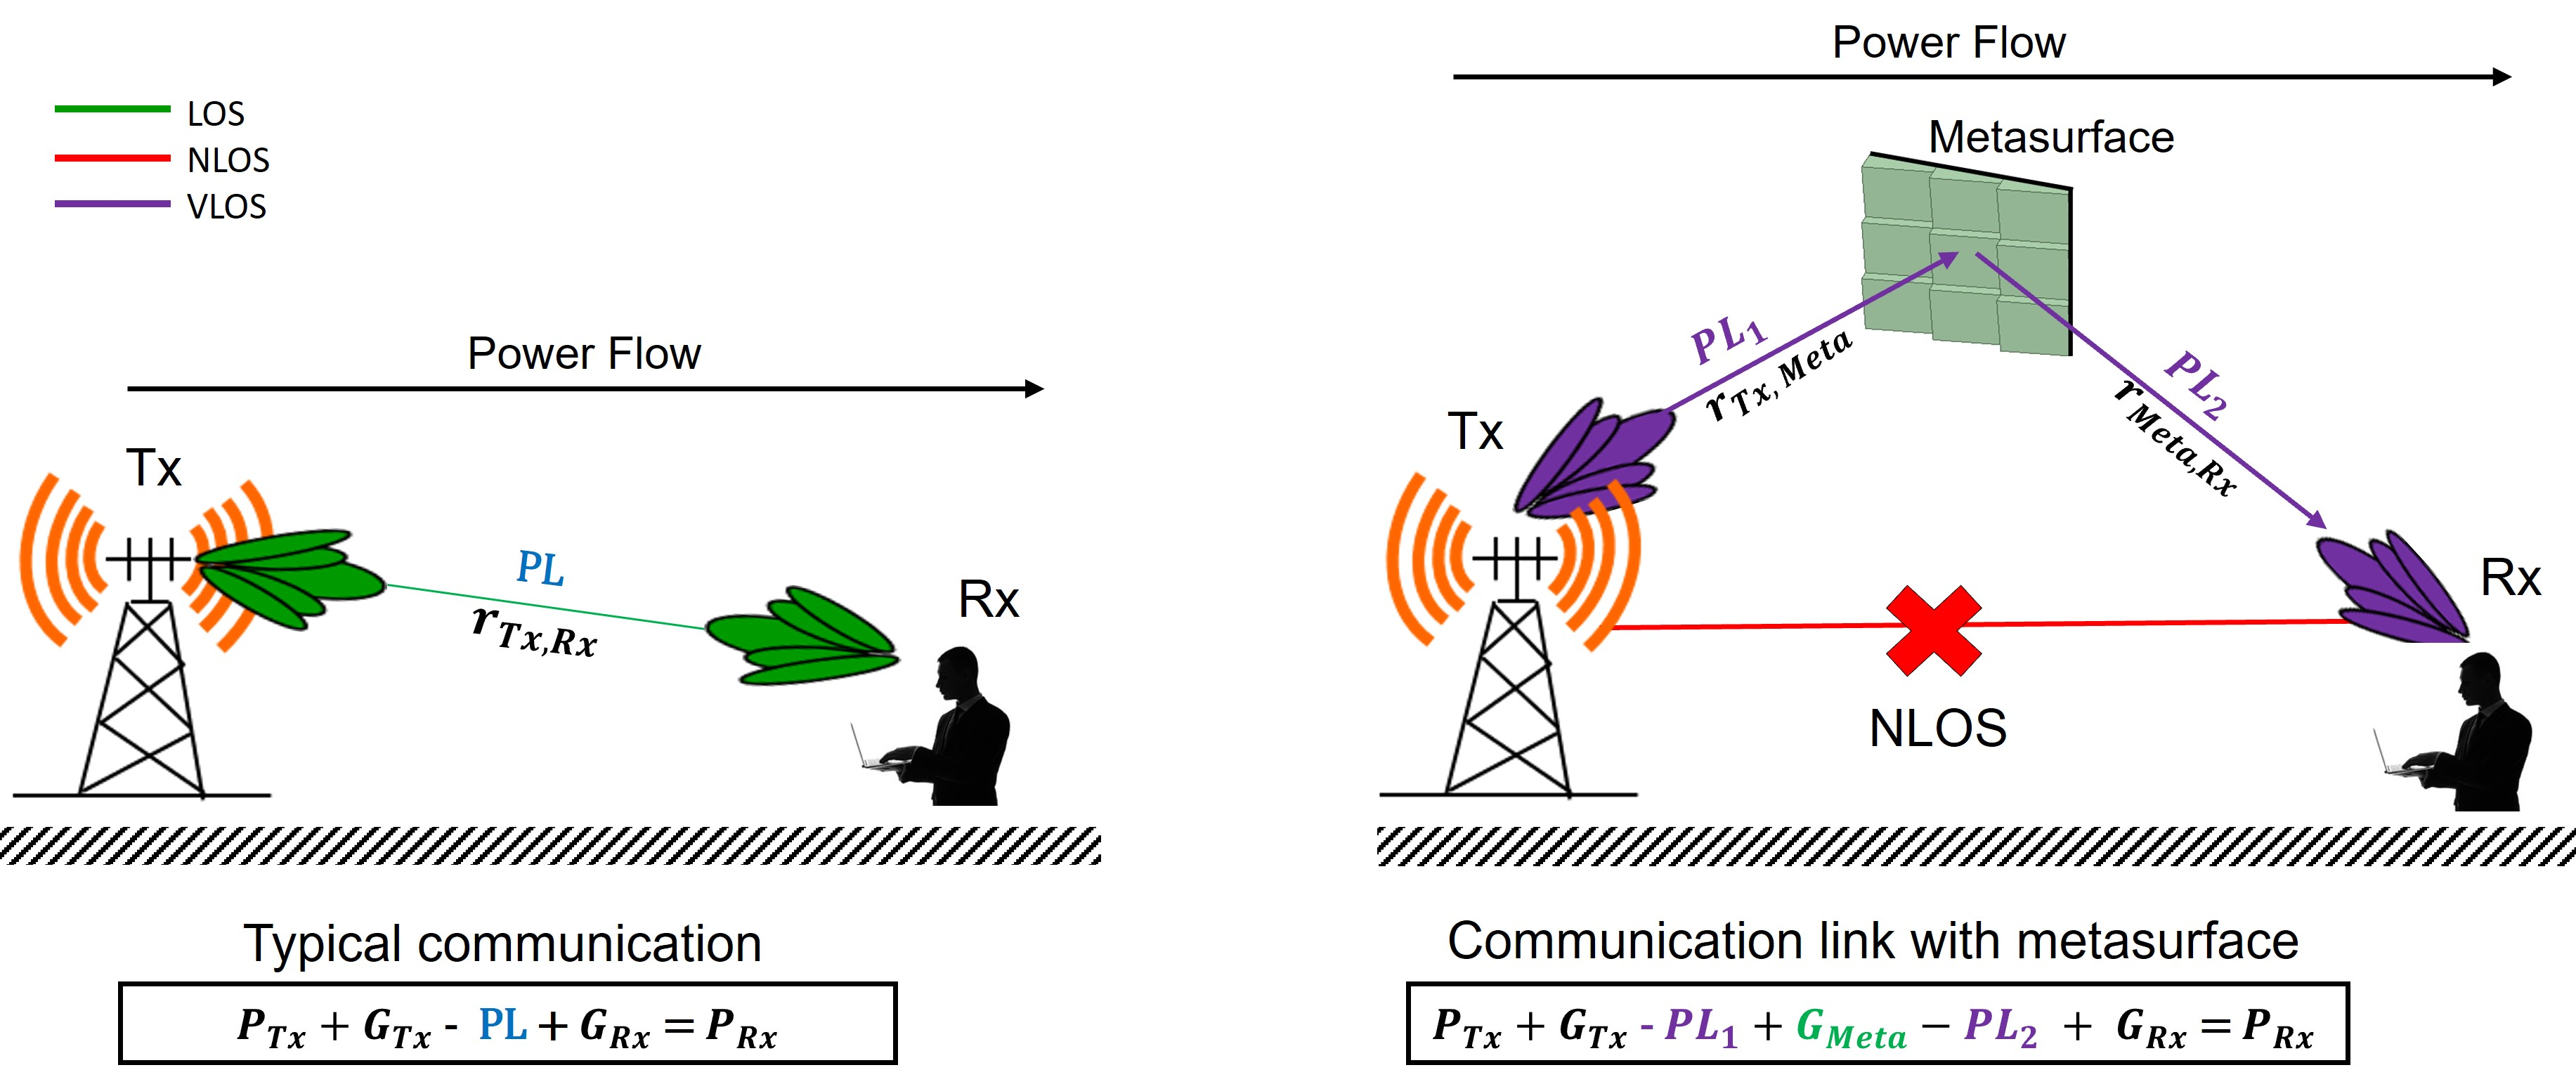
\includegraphics[width=0.9\linewidth]{images/Section 2 Images/Comm_link}
	\caption{Illustration of 6G downlink transmission without (left) and with metasurface (right). In this work, we are particularly interested in deploying IRSs to enable efficient communication in  NLOS regimes by using two LOS subchannels.}
	\label{fig:commlink}
\end{figure}
\Cref{fig:commlink} shows a comparison of the usual communication link without and with metasurface integration. The traditional communication link running from the transmitter to the receiver is depicted on the left side of the figure. The relationship established in this context is defined by classical parameters, i.e., $P_{Tx}$, $P_{Rx}$, $G_{Tx}$, $G_{Rx}$, and $PL$ between them. On the right of \Cref{fig:commlink}, we consider metasurfaces to serve NLOS users. The communication link is established between the transmitter to metasurfaces and, to the receiver. In addition to the classical parameters, we observe two subchannels i.e., Tx-metasurface, and metasurface-Rx, and introduce path losses between them which are given by $PL_{1}$ and $PL_{2}$, which is then compensated by the gain at the metasurfaces $G_{Meta}$.

\begin{figure}[tb]
	\centering
	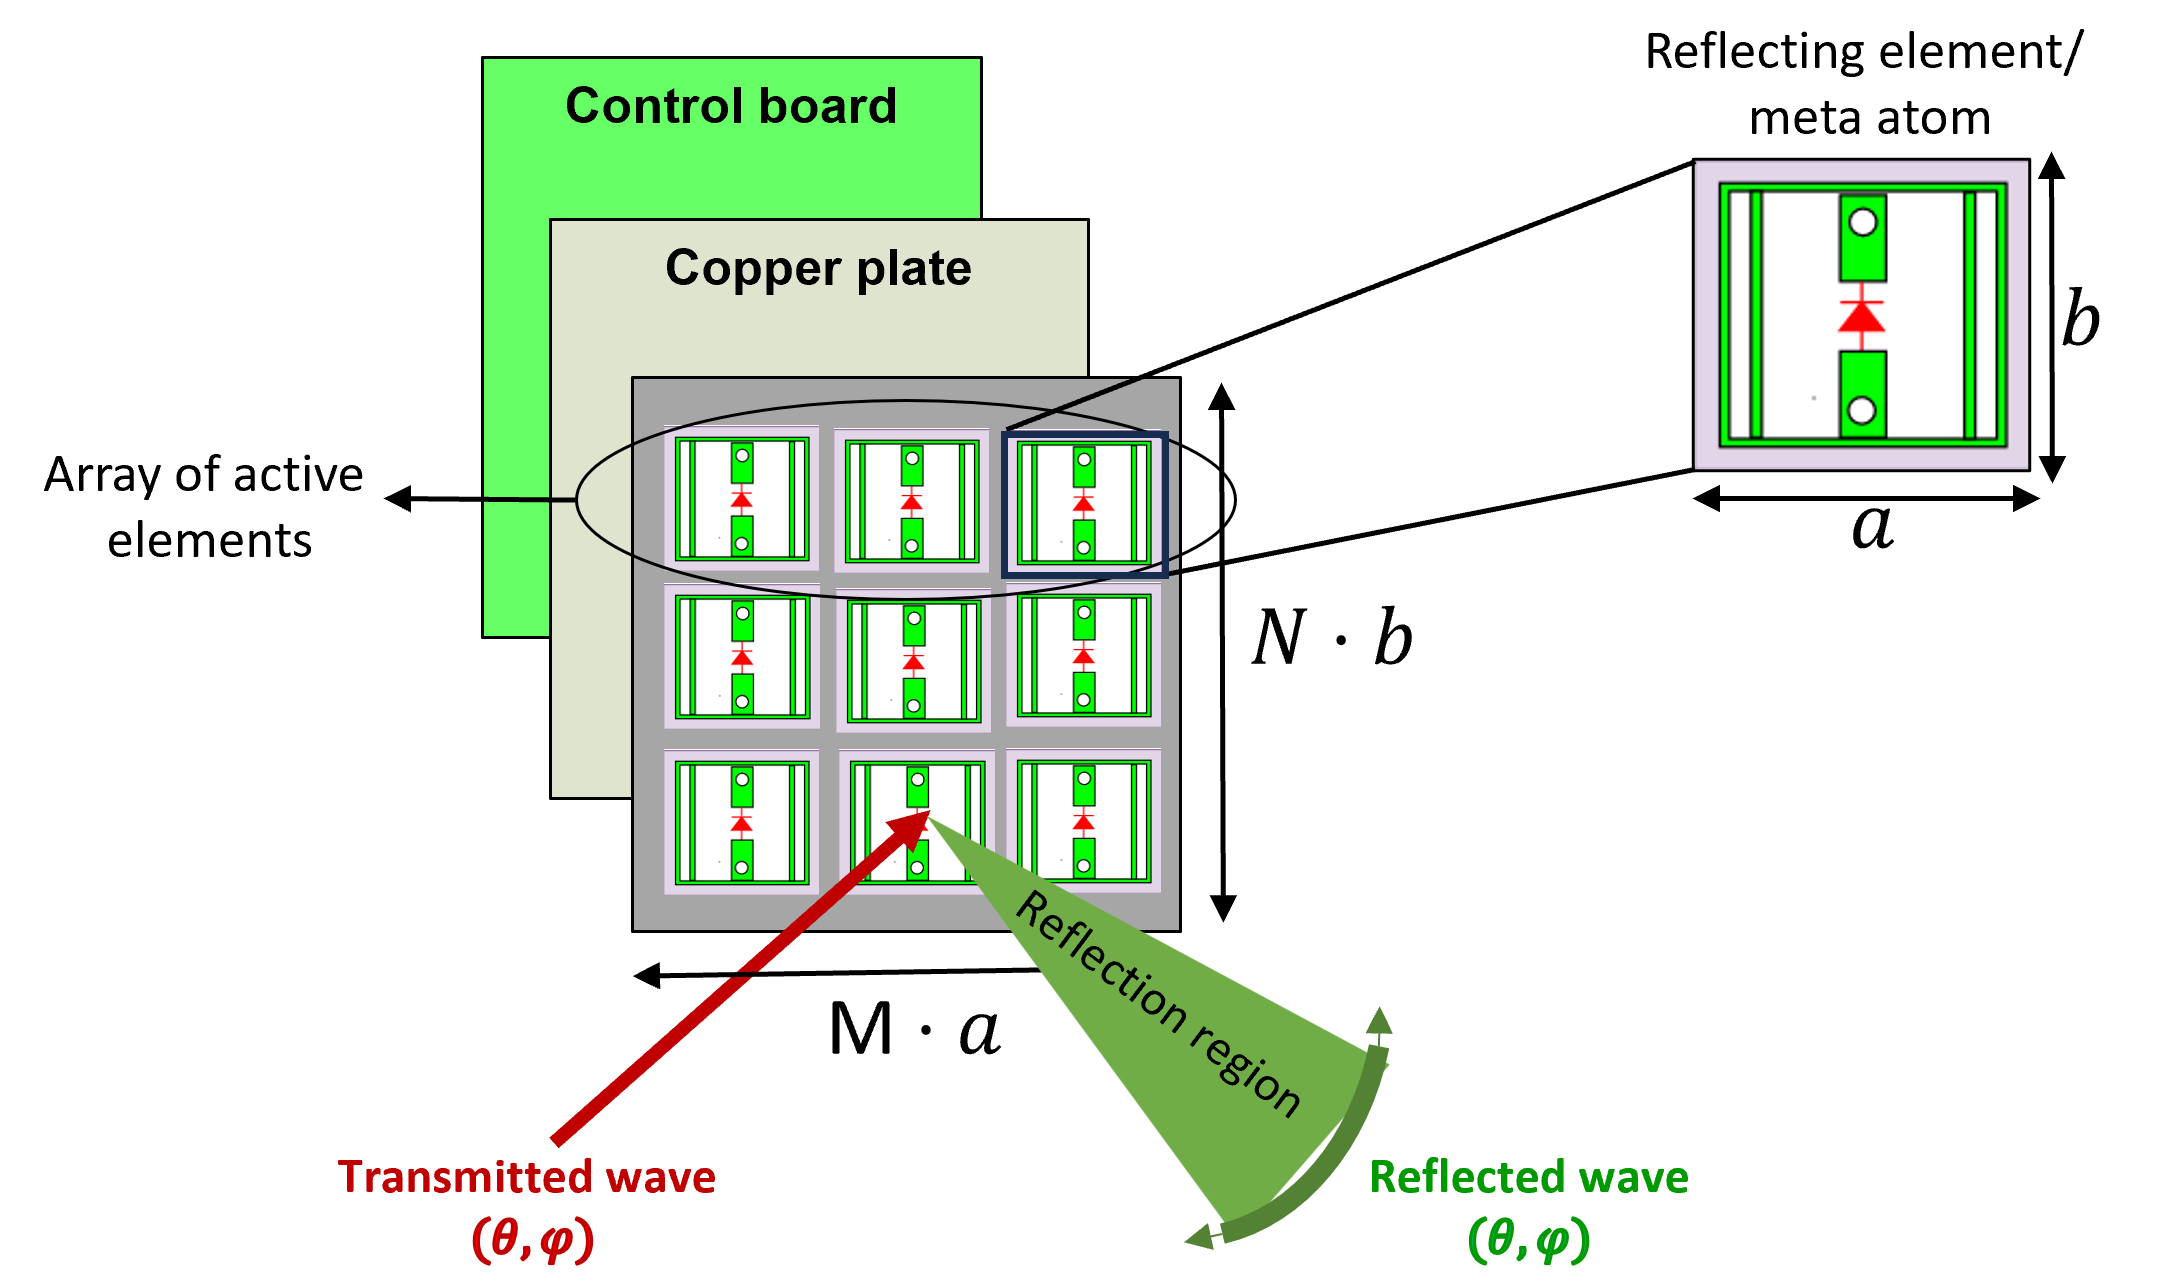
\includegraphics[width=1.0\linewidth]{images/Section 2 Images/IRS}
	\caption{Design and architecture of IRS with an array of active elements where the transmitted wave is reflected in a controllable manner in the reflection region for the overall dimensions of $(M\times a) \cdot (N \times b)$.}
	\label{fig:irs}
\end{figure}
\Cref{fig:irs} depicts the structural architecture of an IRS model. They are made up of sub-wavelength unit cells constituting a planar array of $M \times N$ active elements whose dimensions are $a \times b$, respectively. As mentioned previously, they can alter the interaction between the incident wave and the surface. We will examine two crucial of many feasible crucial metasurface features in more detail in the next sections. First, we consider IRSs in \Cref{IRS}, which may actively direct the reflection into the target direction with the reflection pattern being configured in real-time as desired, focusing on flexibility and adaptability to enhance the coverage and signal strength. Second, we discuss passive reflectors in \Cref{Passive reflectors}, which are entirely passive in nature, i.e., not reconfigurable, but still provide a customized reflection pattern with zero power consumption.

\subsection{Design and Architecture of Intelligent Reflecting Surfaces} \label{IRS}
\ac{IRS}s contain a variety of tiny, reconfigurable reflecting components, enabling precise shaping of the arising reflection pattern by modifying the phase and amplitude of the reflected waves. When compared to reflect-arrays, \ac{IRS}s are instead placed in the far-field regions of Tx and Rx, i.e., at practical positions such as building facades \cite{IRS_citations}.

The functionality of the \ac{IRS} depends heavily on its design and architecture which are created to be flexible, and scalable for a variety of wireless applications as shown in  \Cref{fig:irs}. An \ac{IRS} typically consists of a planar array of unit cells whose dimensions are $a \times b$. These may modify the characteristics of electromagnetic waves' phase, amplitude, and polarization \cite{wu2019towards}. The performance metrics depend on, e.g., the spacing density and number of control bits of the unit cells. These parameters, but also the IRS material affect the supported carrier frequency and bandwidth. Most important, however, is the setting of each unit cell, e.g., in terms of phase as the superposition of the individual unit cells' interactions with the incident EM wave yields the overall IRS performance. Determination of these settings is the main design factor for real-time operation \cite{IRSdesignandapp, Shen2020ModelingAA, wu2019towards}.

6G use cases for IRSs are, for example, as follows: To increase signal strength and coverage inside a building, for instance, one to several \ac{IRS}s can be mounted on available wall sections or the ceiling \cite{IRSdesignandapp}. This way, fewer antenna sites are required such that costs and power consumption are reduced. An \ac{IRS} can also be used to lessen interference to further enhance the quality of wireless communications. Other usage concepts envision improved security and privacy for wireless communications by, in essence, building a physical barrier that prevents signals from being intercepted or eavesdropped. 

Considering the active elements, IRSs need a power line or battery for continuous operation. Additionally, the IRS needs to be controlled by the network operator via a wired link or a wireless connection to the Tx. As an IRS numerous unit cells can form reflection beams similar to an antenna array forming pencil or sector beams, these configurations shall be provided by the network operator along the control link \cite{IRS_citations2}. For this purpose, however, novel signaling procedures similar to the beam management described in \Cref{Millimeter wave communication} is required for 6G.
\subsection{Passive Reflectors and the HELIOS Concept} \label{Passive reflectors}
However, there are some real-world difficulties with the \ac{IRS}, such as the need to deal with the complexity of hardware implementation, scalability, and rising energy consumption with size. While \ac{IRS} represents an evolution for future 6G communications in wireless communication, passive reflectors present a scalable, non-reconfigurable alternative feasible in the short term. In contrast to active IRSs, passive reflectors may not amplify signals but either bundle or scatter the incident energy into a predetermined and fixed direction. Passive reflectors can be created like the metasurfaces outlined in \Cref{IRS} \cite{LiSinghSievenpiper, FangLiChenSunXiaoHeZhou}, but without the use of adjustable unit cells. Alternative techniques, such as HELIOS \cite{Helios}, are also conceivable as explained below.
\subsubsection{Introduction of HELIOS Concept} \label{Introduction of HELIOS Concept}
In light of the previously discussed drawbacks of IRSs, passive reflectors have some advantages over \ac{IRS} in certain situations. The majority of passive reflectors posses typically fixed structures made up of strategically placed metallic surfaces or objects \cite{Anjinappa, Passiverefl}. Their position and geometry can be deliberately exploited to realize the desired reflection behavior as needed to optimize the communication performance. Naturally, their fixed position and shape make them compatible with existing wireless communication systems as there is no need for novel control links and signaling procedures, while also removing the need for a power supply. Thus, the advantage comes in the simplicity which is expected to also reduce costs. Moreover, passive reflectors are expected to be very dependable for tough outdoor settings coming with challenges regarding temperature (hot and cold), moisture, UV radiation, and wind.

Passive reflectors, in this work represented by the HELIOS \cite{Helios} concept, come with the above-described features and may quickly revolutionize the wireless network infrastructure landscape. The core approach is as follows:
\begin{itemize}
	\item Seamless, piecewise installation that easily merges into urban settings without imposing any power supply demands.
	\item Sleek design and manufacturing method not only meets network operators’
	rigorous criteria but also improves network coverage capabilities.
	\item The combination of passive reflectors with cutting-edge processes such as 3D printing and precise spray painting opens up new options for customization and adaptability.
\end{itemize}
\begin{figure}[tb]
	\centering
	\subfloat[$2 \times 2$ HELIOS reflector array with $a=\SI{10}{\centi\meter}$, $b=\SI{5}{\centi\meter}$, $\alpha_{m,n}=20^\circ$, and $\beta_{m,n}=10^\circ$.]{
		\includegraphics[width=0.3\linewidth]{images/Section 2 Images/model_2x2}
		\label{fig:model_2x2}
	}
		\hfill
	\subfloat[$4 \times 1$ HELIOS reflector array with $a=\SI{20}{\centi\meter}$, $b=\SI{10}{\centi\meter}$, $\beta_{m,n}=10^\circ$, and $\alpha_{1,1},\dots,\alpha_{4,1}=(5,10,15,20)^\circ$.]{
		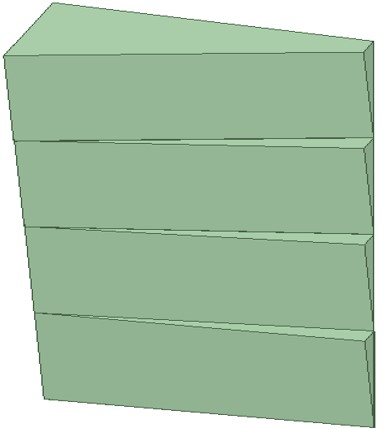
\includegraphics[width=0.3\textwidth]{images/Section 2 Images/model_4x1}
		\label{fig:model_4x1}
	}
		\hfill
	\subfloat[$8 \times 8$ HELIOS reflector array with $a=\SI{10}{\centi\meter}$, $b=\SI{15}{\centi\meter}$, $\alpha_{m,n}=10^\circ$, and $\beta_{m,n}=15^\circ$.]{
		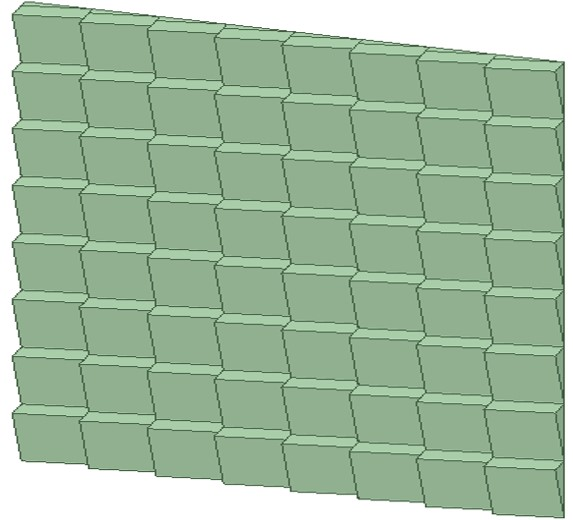
\includegraphics[width=0.3\textwidth]{images/Section 2 Images/model_8x8}
		\label{fig:model_8x8}
	}
	\caption[Illustration of HELIOS reflector arrays with different dimensions, sizes, and slope angles, showcasing the high degree of flexibility of the model.]{Illustration of HELIOS reflector arrays with different dimensions, sizes, and slope angles, showcasing the high degree of flexibility of the model.}
	\label{fig:model_array}
\end{figure}
We will now delve into the authors' design and production process for their HELIOS reflectors. The first step constitutes the careful selection of a suitable geometry, i.e., one with the capacity to successfully reflect the incident electromagnetic wave into the desired direction range. Another critical component of the geometry design is its unobtrusiveness, i.e., minimization of the exhibited protrusion for better technology acceptance \cite{Helios}. Following that, the authors choose suitable materials and production processes depending on the deployment scenario under aspects of durability, resource efficiency, and costs.

The HELIOS reflector array's adaptation to various configurations, which display a range of dimensions, reflector sizes, and slope angles, is a testament to its versatility as illustrated in \Cref{fig:model_array}. The versions that are shown have different values, which highlights the amazing adaptability that the design offers. Because of its adaptation to many settings, this variability highlights the model's versatility and enables customization depending on unique requirements, making it a highly flexible model.
\subsubsection{Construction of Geometry of HELIOS Reflector Module}
The primary principle controlling the geometry selection of the reflector is the application of Snell's law of reflection \cite{7728465}. When dealing with a flat reflecting plate with dimensions $a \times b$, our method involves an incident wave meeting the surface at azimuth and elevation angles, with the reflected wave preserving identical angles relative to the surface normal, cf. \Cref{fig:HELIOS1}. As we move into the domain of three-dimensional passive reflectors, the problem becomes custom-tailoring these structures to precisely focus the transmitted beam towards the specified receiver direction, by the criteria of our network planning.

To accomplish this, the authors designed a saw-tooth-like structure for the reflector, with the depth of each protrusion decreasing proportionally as the number of modules grows \cite{Helios}. \Cref{fig:HELIOS2}, and \Cref{fig:HELIOS3} illustrate the impact of an individual module's horizontal tilt angle $\alpha$ on the azimuth reflection angle $\varphi_{out}$ and, in addition, the joint case in which a vertical slope angle $\beta$ further affects the elevation reflection angle $\theta_{out}$. It is worth mentioning that the parametrization of the reflector
\begin{figure}[H]
	\centering
	\subfloat[Basic rectangular flat plate with no element of slope angles with the depiction of Snell's law of reflection.]{
		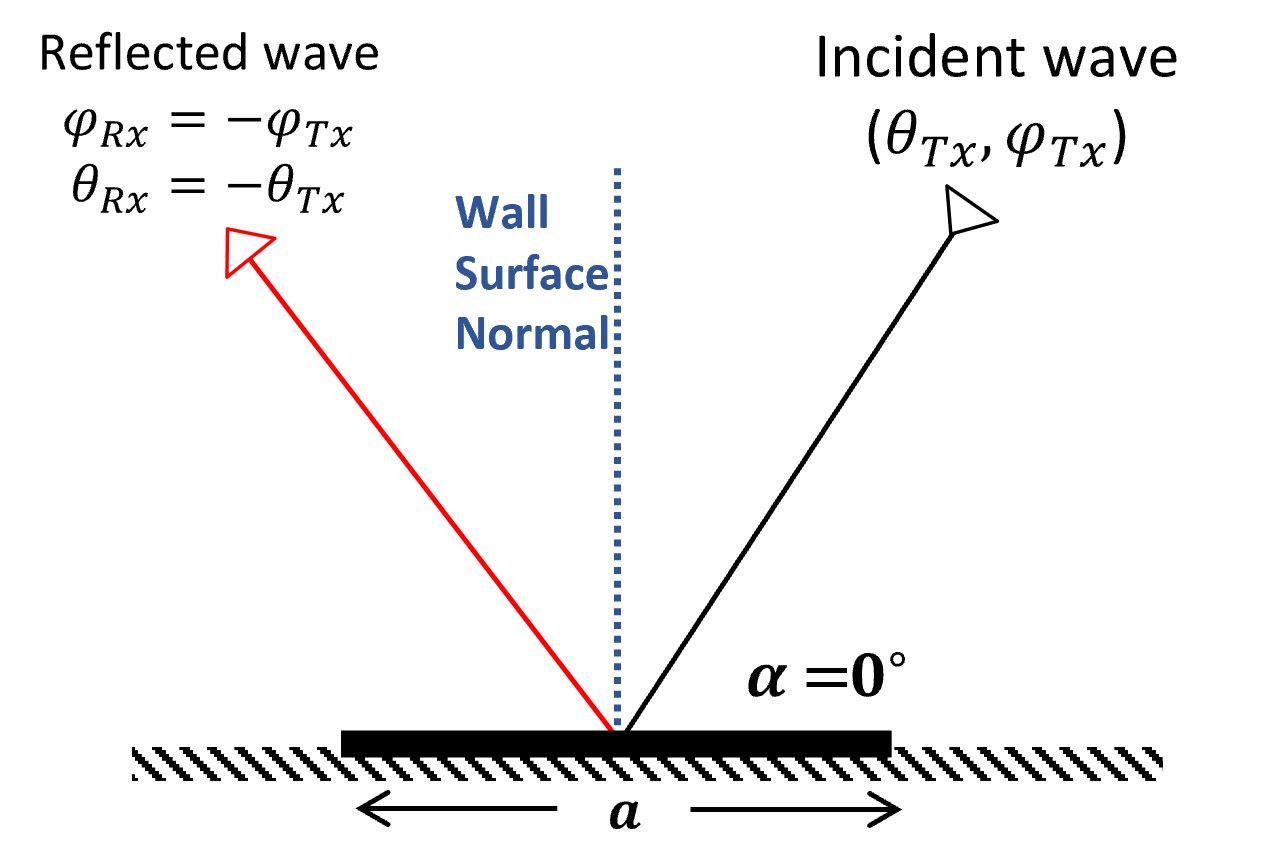
\includegraphics[width=0.3\linewidth]{images/Section 2 Images/HELIOS_1}
		\label{fig:HELIOS1}
	}
	\hfill
	\subfloat[HELIOS module with slope angle $\alpha$ with a height $h$, depicting the shift in the reflected wave by two times the $\varphi_{Tx}$.]{
		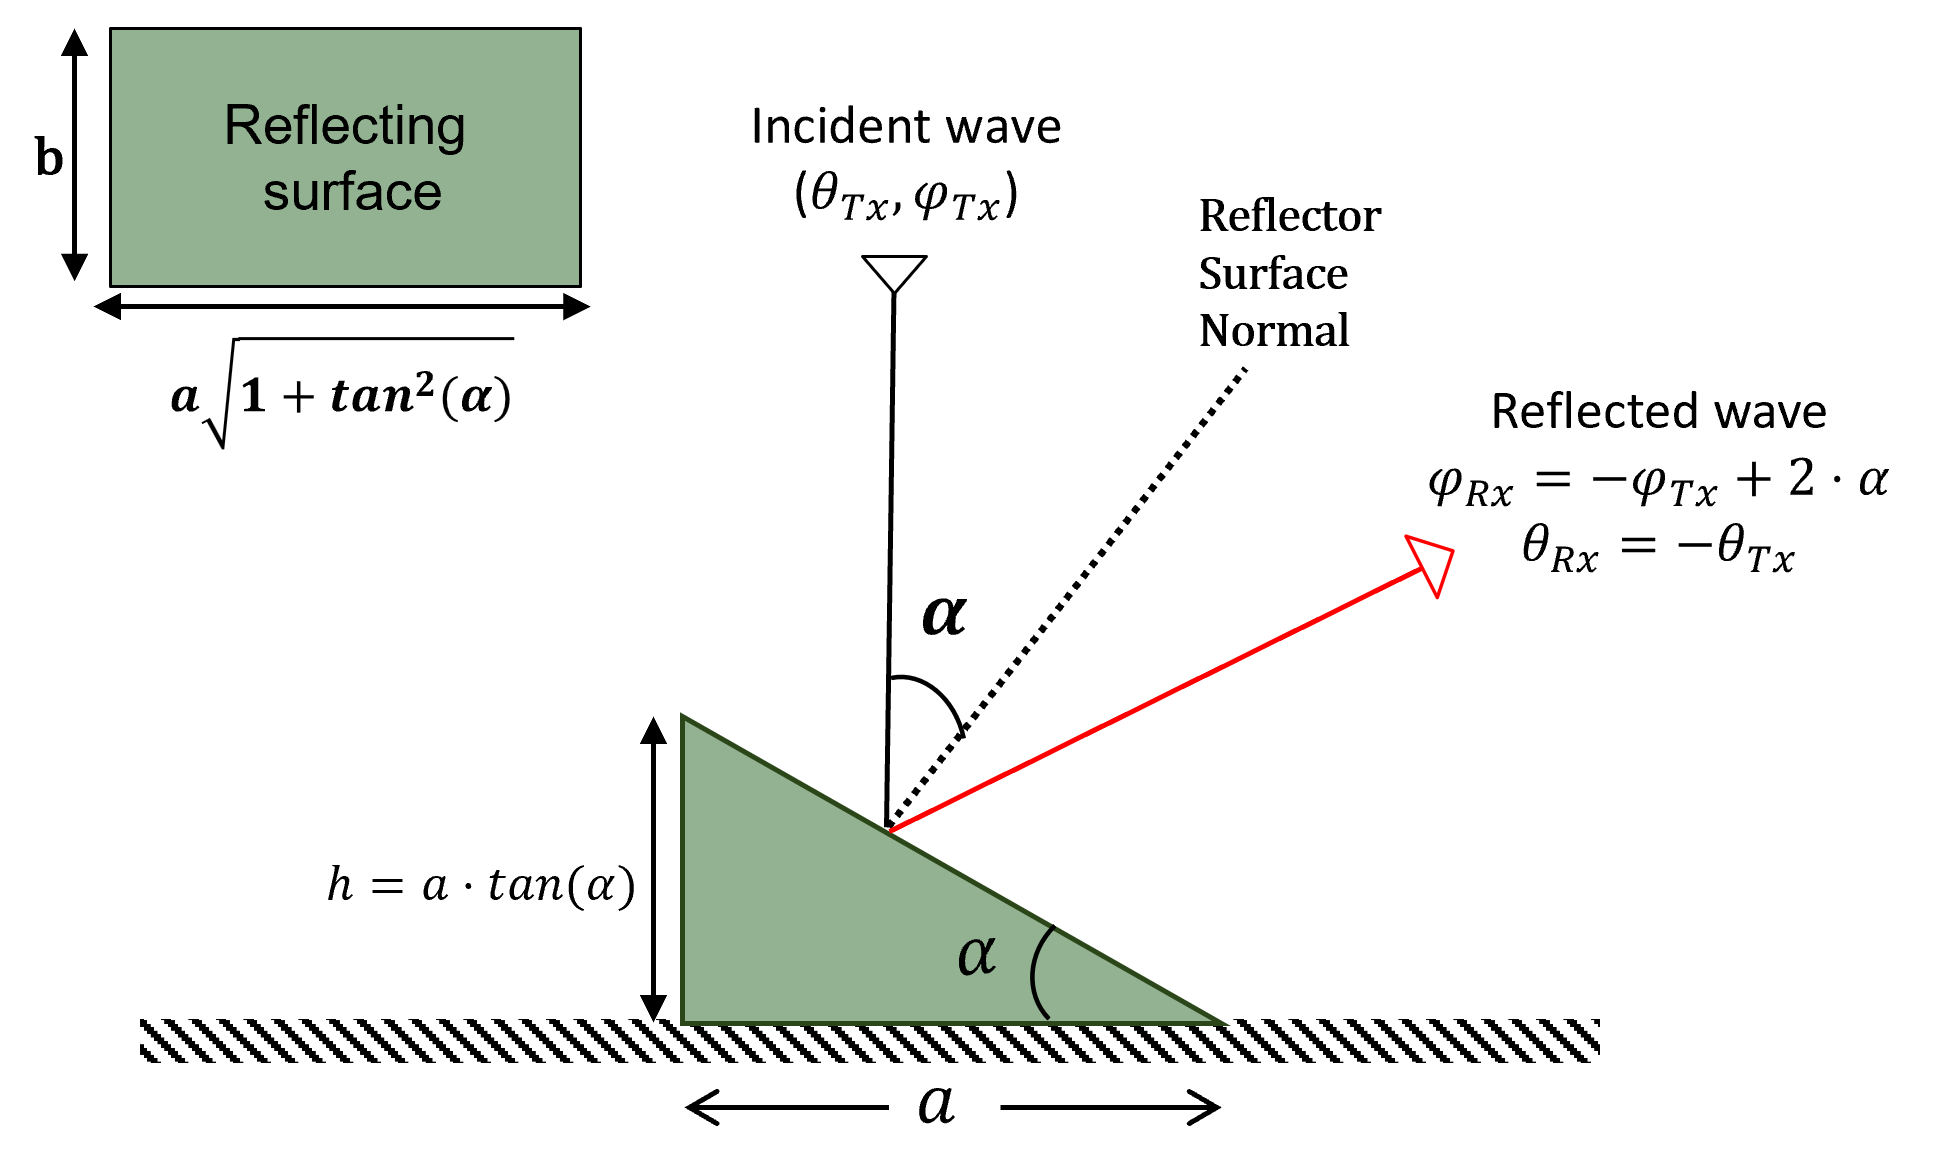
\includegraphics[width=0.3\textwidth]{images/Section 2 Images/HELIOS_2}
		\label{fig:HELIOS2}
	}
	\hfill
	\subfloat[HELIOS module with slope angle $\alpha$ and $\beta$ with a height $h$, depicting the shift in the reflected wave by two times the $\varphi_{Tx}$ and $\theta_{Tx}$.]{
		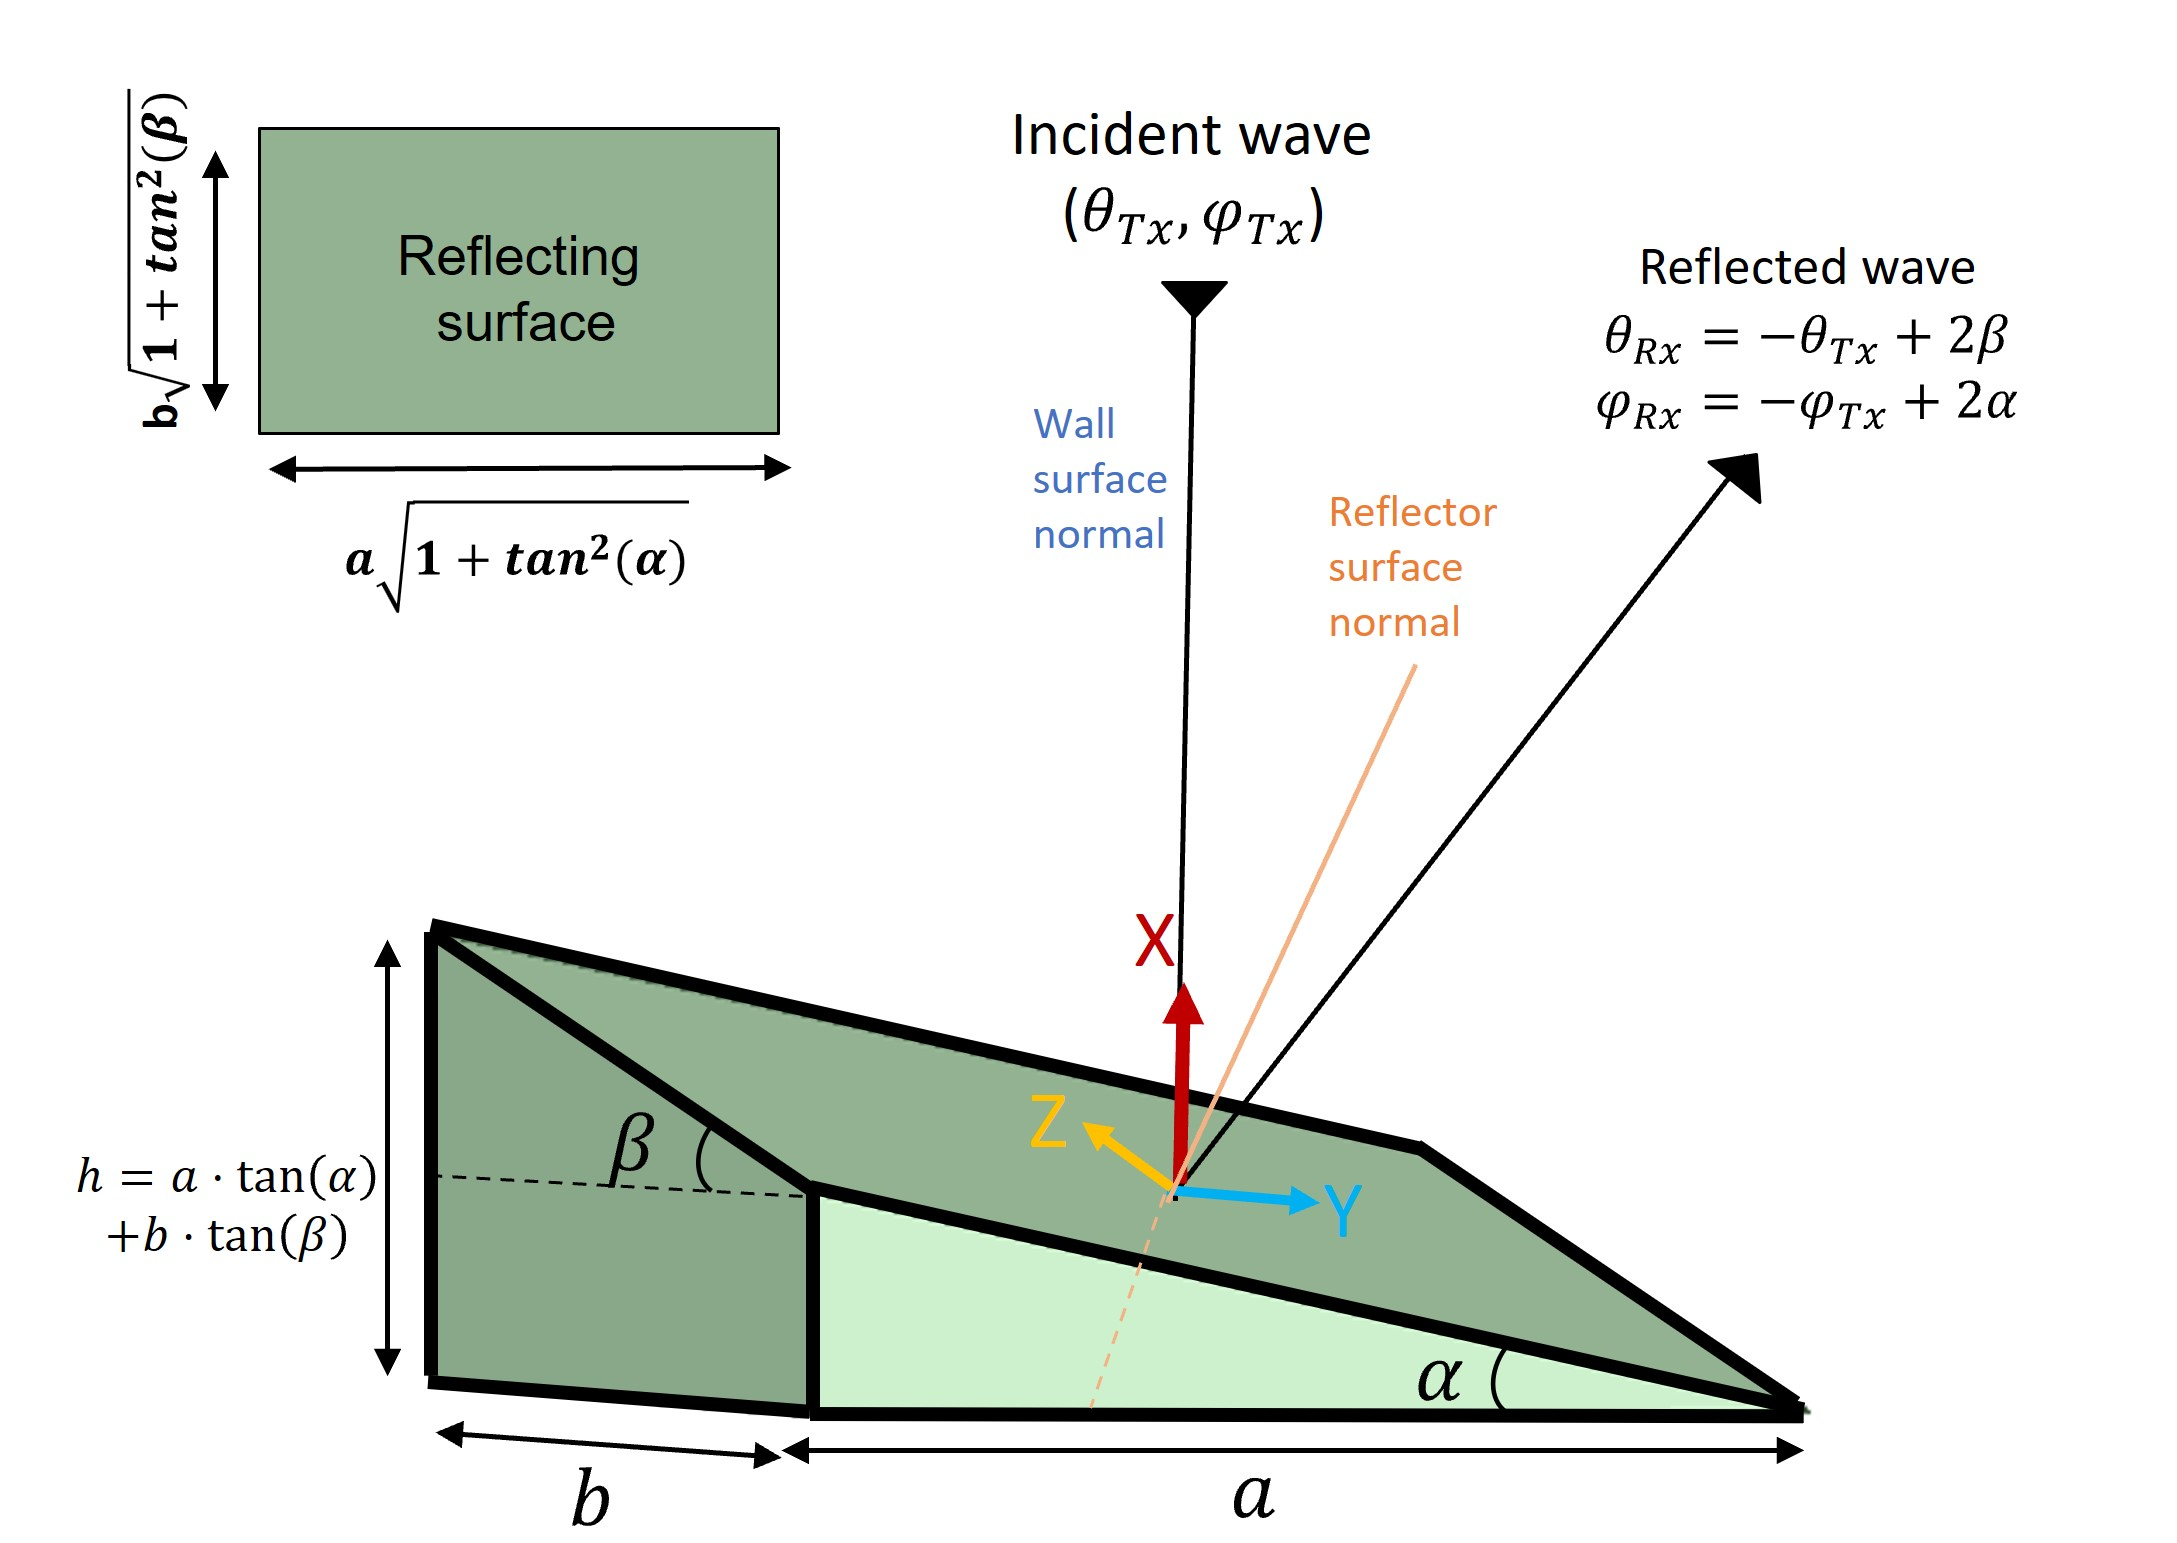
\includegraphics[width=0.32\textwidth]{images/Section 2 Images/HELIOS_3}
		\label{fig:HELIOS3}
	}
	\caption[Horizontal and vertical tilting of the reflecting surface enables deliberate steering of the reflection towards the desired direction.]{Horizontal and vertical tilting of the reflecting surface enables deliberate steering of the reflection towards the desired direction. }
	\label{fig:tricdvsuq}
\end{figure}
module, which includes variables such as vertical and horizontal slope angles namely $\alpha_{m,n}$ and $\beta_{m,n}$, reflector element base size $a \times b$, and indices $m \in 1, \dots, M$ and $n \in 1, \dots, N$ with $M \times N$ specifying the number of HELIOS modules.
\subsubsection{Material Selection}
Reflectors are often made of highly conductive materials to minimize signal loss. While traditional options such as solid metal reflectors or aluminum foil are effective, they come with high material prices \cite{Helios}. Moreover, reshaping supplies of metal into the desired HELIOS form may complicate production, and thus, increase costs. The HELIOS concept addresses these issues as follows. Using 3D printing with a suitable filament, e.g., PLA for indoor deployments, arbitrary shapes may be produced. Afterward, a conductive coating is given via spray-coating.
\subsection{Common Coordinate System and Parameters for Metasurface Characterization} \label{coordinate systems}
The investigation of metasurfaces for \ac{mmWave} communication leverages the subsequently described cartesian reference coordinate system, as illustrated in  \Cref{fig:3D model}. A 3D space defined by the three perpendicular axes ($x,y$, and $z$) in this coordinate system, which enables us to precisely find and describe the position and orientation of components in wireless communication systems. For example, the reflecting surface shall be in the $y$-$z$-plane.

Let us consider a planar EM wave impinging on the reflecting surface. The direction of this wave is indicated by its wave vector $\overrightarrow{\textbf{k}}$ which can be related to the direction of the normal vector $\overrightarrow{\textbf{n}}$ of the surface \footnote{Note that vector n has a positive z-component, otherwise, the vector would point into the building or ceiling at which the reflector is mounted.}. As depicted by  \Cref{Vectork} vectors $\overrightarrow{\textbf{k}}$ and $\overrightarrow{\textbf{n}}$ can be described relative to the reflecting surface using spherical coordinates, namely azimuth angle $\varphi_k \in [-180:180]^\circ$ (defined in $y$-$z$-plane from $y$-axis in the direction of $z$-axis) and elevation angle $\theta_k \in [-90:90]^\circ$ (defined in $y$-$z$-plane towards $x$-axis), as well as the magnitudes $n$=\num{1} and $k= \frac{2 \cdot \pi}{\lambda}$.
\begin{equation} \label{Vectork}
	\begin{split}
		\overrightarrow{\textbf{k}} &= (k, \theta_{k}, \varphi_{k})\\
		\overrightarrow{\textbf{n}} &= [1, 0, 0]
	\end{split}
\end{equation}
Using the described parameters, we describe vector $\overrightarrow{\textbf{k}}$ in Cartesian coordinates as follows:
\begin{figure}[tb]
	\centering
	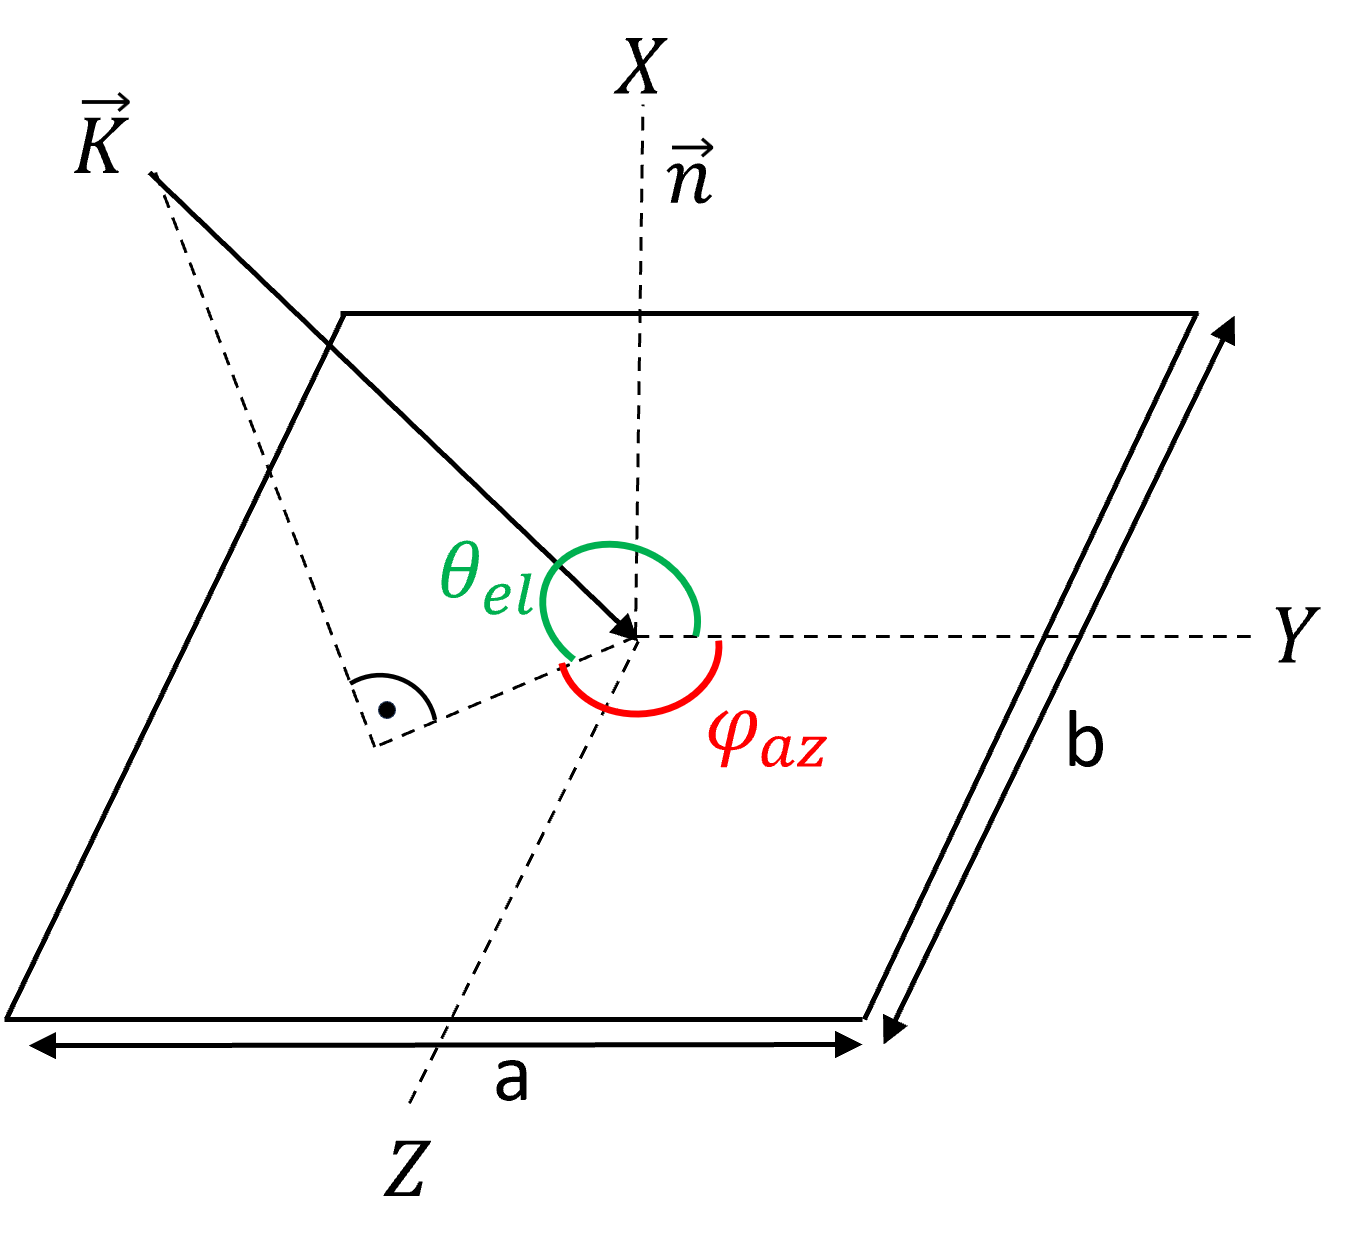
\includegraphics[width=0.5\linewidth]{images/Section 2 Images/coordinate_system}
	\caption{Plane wave impinges along direction k on reflecting surface in $y$-$z$-plane with elevation angle $\theta_{el}$ and azimuth angle $\varphi_{az}$ in \si{\deg}.}
	\label{fig:3D model}
\end{figure}
\begin{equation} \label{Eq:Coordinates conversion of impinging wave vector_1}
	\overrightarrow{\textbf{K}} =
	\begin{bmatrix}
		k_x\\ k_y\\k_z
	\end{bmatrix}
	= k
	\begin{bmatrix}
		\cos(\theta_{k}) \cdot  \cos(\varphi_{k})  \\ 
		\cos(\theta_{k}) \cdot \sin(\varphi_{k})\\
		\sin(\theta_{k})
	\end{bmatrix}
\end{equation}
Furthermore, we may deduce the spherical coordinate system parameters from the Cartesian description as follows:
\begin{equation} \label{Eq:theta_inc and varphi_inc}
	\begin{split}
		\theta_{k} &= \arccos{\frac{k_z}{|\overrightarrow{\textbf{k}}|}} \\
		\varphi_{k} &= \arctan{\frac{k_y}{k_x}} 
	\end{split}
\end{equation}
where $|\overrightarrow{\textbf{k}}|$ is the magnitude of impinging wave vector $\overrightarrow{\textbf{k}}$.
\begin{equation}
	|\overrightarrow{\textbf{K}}|= k= \sqrt{k_x^2+ k_y^2+ k_z^2}
\end{equation}
In the following, we will refer to the incident  wave vector using $\overrightarrow{\textbf{K}_{Tx}}$, whereas the reflected wave uses $\overrightarrow{\textbf{K}_{Rx}}$. Based on the law of reflection, the angle of the incident is implicitly defined by the reflection angle, given by \Cref{Eq:law of reflection}. So, the elevation and azimuth angles of the impinging and reflecting waves will have the same magnitude but different signs.
\begin{equation} \label{Eq:law of reflection}
	\begin{split}
		\theta_{Rx} &= -\theta_{Tx}\\
		\varphi_{Rx} &=  -\varphi_{Tx}
	\end{split}
\end{equation}
Let us consider the Euclidean norm angles to be $\gamma_{Tx}$ and $\gamma_{Rx}$ at the transmitter and the receiver, respectively. As defined in  \Cref{Eq:euclidean norm}, they define the overall deviation angle from the $x$-axis.
\begin{equation} \label{Eq:euclidean norm}
	\begin{split}
		\gamma_{Tx} &= \sqrt{\theta_{Tx}^2+\varphi_{Tx}^2}\\
		\gamma_{Rx} &= \sqrt{\theta_{Rx}^2+\varphi_{Rx}^2}
	\end{split}
\end{equation}
In the following sections, the previous metasurface geometry relations will be applied. \Cref{Variable abbreviation} extends these with additional parameters incorporating the above geometry into a wide communication system description including the Tx and Rx.
\begin{table}[H] % H -> dieses objekt wird genau da wo der code steht festgenagelt
	\footnotesize
	\caption{Comprehensive standardization of parameters: Units and abbreviations for metasurface channel modeling across the entire thesis.}
	\label{Variable abbreviation}
	\centering
	\begin{tabular}{C{3cm}|C{7cm}|C{2.5cm}}
		\textbf{Abbreviation} & \bf Definition & \bf Units\\
		\hline 
		$\eta$ & Characteristic impedance & $\Omega$\\
		\hline 
		$f$ & Frequency & \si{\hertz} \\
		\hline 
		$c$ & Speed of light & \si{\meter}/\si{\second} \\
		\hline
		$\Gamma$ & Reflection coefficient & Unitless\\
		\hline 
		$k$ & Wave number & \si{\per\meter}\\
		\hline
		$\lambda$ & Wavelength & \si{\meter}\\
		\hline 
		$a$  & $y$-axis dimension of the \ac{IRS} & \si{\meter} \\
		\hline 
		$b$  & $z$-axis dimension of the \ac{IRS} & \si{\meter} \\
		\hline 
		$M$  & Reflector array on the $z$-axis of the \ac{IRS} & Unitless \\
		\hline 
		$N$  & Reflector array on the $y$-axis of the \ac{IRS} & Unitless \\
		\hline 
		$A_{eff}$ & Effective aperture of the \ac{IRS}  & $\si{\meter}^2$\\
		\hline 
		$ E_{incident}$  & Electric field strength of the incident signal & $V/\si{\meter}$\\
		\hline 
		$ E_{reflect}$  & Electric field strength of the reflected signal & $V/\si{\meter}$\\
		\hline 
		$P_{incident}$ & Power of incident signal & $W$ \\
		\hline 
		$ P_{captured}$ & Power captured by \ac{IRS} element & $W$  \\
		\hline 
		$ P_{reflected}$ & Power reflected by \ac{IRS} element & $W$  \\
		\hline 
		$P_{Rx}$ & Power received by the receiver & $W$ \\
		\hline 
		$ P_{Tx} $  & Transmit power & $W$ \\
		\hline 
		$G_{Tx} $ & Gain of transmit antenna & Unitless\\
		\hline 
		$G_{Rx} $ & Gain of receiver antenna & Unitless\\
		\hline
		$G_{IRS}$ & Gain of \ac{IRS} & Unitless \\
		\hline 
		$r_{Tx,Rx}$ & Distance from transmitter to receiver & \si{\meter}\\
		\hline 
		$r_{Tx,IRS}$ & Distance from transmitter to \ac{IRS} element & \si{\meter}\\
		\hline 
		$r_{IRS,Rx}$ & Distance from receiver to \ac{IRS} element & \si{\meter} \\
		\hline 
		$\theta_{Tx}$ & Elevation angle to the transmitter & \si{\deg}\\
		\hline 
		$\varphi_{Tx} $  & Azimuth angle to the transmitter & \si{\deg} \\
		\hline 
		$\theta_{Rx}$ & Elevation angle to the receiver & \si{\deg}\\
		\hline 
		$\varphi_{Rx} $  & Azimuth angle to the receiver & \si{\deg} \\
		\hline 
		$\theta_{dev}$ & Deviated elevation angle at the receiver & \si{\deg}\\
		\hline 
		$\phi_{dev} $  & Deviated azimuth angle at the receiver & \si{\deg} \\
		\hline 
		$\Phi_{IRS} $  & Phase shift by IRS unit cell & \si{\deg} \\
		\hline 
		$\gamma_{Tx}$ & Overall IRS angle of incidence & \si{\deg}\\
		\hline 
		$\gamma_{Rx} $  & Overall IRS angle of reflection & \si{\deg}\\
		\hline 
		$PL$ & Path loss & Unitless\\ 
		\hline
		$SNR$ & Signal-to-Noise ratio & Unitless\\
		\hline
		$\alpha$ & Elevation slope angle & \si{\deg}\\
		\hline 
		$\beta$ & Azimuth slope angle & \si{\deg}\\
		\hline 
		$Gain_{RCS} $ & Analytical gain at the reflector & \si{\decibel} \\
		\hline 
		$Gain_{Sim} $ & Simulated gain at the reflector & \si{\decibel}\\
	\end{tabular}
\end{table}
Now that we have a firm grasp of the coordinate system and the variables that will direct our study, we introduce three IRS channel models from the literature and examine each individually.
\subsubsection{Model by Özdogan \emph{et al}. (2020) \cite{8936989}} \label{Model 1}
For an \ac{IRS} that is set up to reflect an incoming wave from a far-field source in a beamforming like manner towards a far-field receiver in direction $\theta_{Rx}$, the authors in \cite{8936989} have used the physical optics approach to derive an end-to-end path loss expression. The model consists of a plate in the $x$-$y$-plane with dimensions $a \times b$ which is perfectly conducting. It is radiated upon with a linearly polarized EM wave at distance $r_{Tx, IRS}$ at angle $\theta_{Tx}$ between incident wave vector and $\overrightarrow{e_z}$, with $\theta_{Tx} \in [0, \frac{\pi}{2}] $. The whole setup can be seen in  \Cref{fig:model1}. In the following we briefly summarize the key results of the work in the form of two lemmas yielding equations that will be used in the scope of this thesis.

Due to its far-field nature, the impinging wave vector is a nearly plane wave and the distribution of the \ac{EM} fields for the incident plane wave is given by  \Cref{Eq:model1 EM_inc} where $\eta$ is the characteristic impedance of the medium.
\begin{equation} \label{Eq:model1 EM_inc}
	\begin{aligned}
		\overrightarrow{E}_{incident} &= E_{incident} \cdot e^{-j \cdot k \left( \sin{\theta_{Tx}} \cdot y - \cos{\theta_{Tx}} \cdot z \right) } {\overrightarrow{e_x}} \\
		\overrightarrow{H}_{incident} &= - \frac{E_{incident}}{\eta} \left( \cos{\theta_{Tx}} \cdot {\overrightarrow{e_y}} +\sin{\theta_{Tx}} \cdot {\overrightarrow{e_z}} \right) \cdot e^{-j \cdot k \left( \sin{\theta_{Tx}} \cdot y - \cos{\theta_{Tx}} \cdot z \right)}
	\end{aligned}
\end{equation}
The E-field will cause the plate's electrons to move and it'll only be in the $\overrightarrow{e_x}$ direction as they are orthogonal. A scattered wave is created as a result of the \ac{EM} radiation that the moving electrons produce.
\begin{figure}[H] % h -> dieses object wird grob in der nähe seines quelltextes erscheinen
	\centering
	\vspace{12pt} %% 12pt abstand zwischen text und grafik
	\includegraphics*[width=0.6\textwidth]{images/Section 2 Images/model1}
	\caption{Illustrating the setup of the IRS model with the 3D angles for the transmitted and reflected wave \cite{8936989}.}
	\label{fig:model1} 
\end{figure}

\textbf{Lemma 1}: Measured against $\overrightarrow{e_z}$, the squared magnitude of the scattered field in the $\overrightarrow{e_y}$, $\overrightarrow{e_z}$ plane, and at any observation angle $\theta_{Dev} \in [0, \frac{\pi}{2}]$ is given by \Cref{Eq:model1 lemma1}.
\begin{equation} \label{Eq:model1 lemma1}
	S(r_{IRS, Rx},\theta_{Dev}) = \left( \frac{a \cdot b}{\lambda} \right)^2 \frac{E_{incident}^2}{r_{IRS, Rx}^2} \cos^2\theta_{Tx} \left[ \sinc \left( \frac{\pi \cdot b}{\lambda}(\sin\theta_{Dev}-\sin\theta_{Tx}) \right) \right]^2
\end{equation}
at a far-field observation distance $r_{IRS, Rx} \geq \frac{2 \cdot max \left( a^2, b^2 \right) }{\lambda}$  \cite{8936989}.

\Cref{Eq:model1 lemma1} has several intuitive properties. For instance, the reflected power is proportional to the squared IRS surface area, i.e., $(a \cdot b)^2$. According to Snell's law, the maximum is attained if the argument of $\sinc=0^\circ$. For $\theta_{Dev} =\theta_{Tx}=0^\circ$ the reflection power is maximized, i.e., an IRS will be most beneficial the more the incident and reflected waves are perpendicular to the surface.

The angles $\theta_{Tx}$ and $\theta_{Dev}$ from earlier represent the ideal case, but the main goal of \ac{IRS} is to achieve total anomalous reflection, with its main beam pointing in the desired direction $\theta_{Rx}$. In order to obtain the ideal field distributions  $\overrightarrow{E}_{reflect}$ and $\overrightarrow{H}_{reflect}$ of the reflected or scattered wave, the surface must be created to divert the incident plane wave as given by  \Cref{Eq:model1 reflect EM}.
\begin{equation} \label{Eq:model1 reflect EM}
	\begin{aligned}
		\overrightarrow{E}_{reflect} &= E_{reflect} e^{-j \cdot k \left( \sin{\theta_{Rx}} \cdot y - \cos{\theta_{Rx}} \cdot z \right) } {\overrightarrow{e_x}}  \\
		\overrightarrow{H}_{reflect} &= - \frac{E_{reflect}}{\eta} \left( \cos{\theta_{Rx}} \cdot {\overrightarrow{e_z}} +\sin{\theta_{Rx}} \cdot {\overrightarrow{e_z}} \right) e^{-j \cdot k \left( \sin{\theta_{Rx}} \cdot y - \cos{\theta_{Rx}} \cdot z \right) }
	\end{aligned}
\end{equation}
\textbf{Lemma 2}: The squared magnitude of the scattered field in \Cref{Eq:model1 squared magnitude of the scattered field} at an arbitrary observation angle $\theta_{Dev} \in [-\frac{\pi}{2}, \frac{\pi}{2}]$ is when using an \ac{IRS} to reflect a signal in the desired direction $\theta_{Rx}$.
\begin{equation} \label{Eq:model1 squared magnitude of the scattered field}
	S(r_{IRS, Rx},\theta_{Dev},E_{incident}) = \left( \frac{a \cdot b}{\lambda} \right)^2 \frac{E_{incident}^2  \cdot \cos^2 (\theta_{Tx})}{r_{IRS, Rx}^2}  \left[ \\sinc \left( \frac{\pi \cdot b}{\lambda} \left(\sin\theta_{Dev}-\sin\theta_{Rx} \right) \right) \right]^2
\end{equation}
The maximum of  \Cref{Eq:model1 squared magnitude of the scattered field} is achieved when $\theta_{Rx}=\theta_{Dev} $, thus confirming that the IRS's reflection is maximized in the desired direction although power is also radiated with varying intensity into other directions. Therefore, this equation includes an important description of the IRS reflection pattern. Notably, it generalizes the hull curve described in \Cref{Eq:model1 lemma1}. With transmitter gain $G_{Tx}$ and receiver gain $G_{Rx}$, \Cref{Eq:model1 E and P } gives the relationship between $E_{incident}$ and transmit power $P_{Tx}$.
\begin{equation} \label{Eq:model1 E and P }
	\frac{E_{incident}^2}{2 \eta} = \frac{P_{Tx} \cdot G_{Tx}}{4 \cdot \pi \cdot r_{Tx,IRS}^2}     
\end{equation}
The effective area $A_{eff} $ of the receiver antenna, also known as the aperture, can be described as follows:
\begin{equation}\label{Aeff}
	A_{eff} = \frac{\lambda^2}{4 \cdot \pi} G_{Rx}
\end{equation}
Coupling \Cref{Eq:model1 squared magnitude of the scattered field}, \Cref{Eq:model1 E and P }, and \Cref{Aeff}, yields \Cref{Eq:model1 power received}, and \Cref{Eq:model1 path loss} as the description of the received power of the IRS-based propagation path. 

\begin{equation} \label{Eq:model1 power received}
	P_{Rx} \left( P_{incident}, r_{Tx, IRS},r_{IRS, Rx},\theta_{Dev} \right) = \frac{1}{2 \cdot \eta} S \left( r_{IRS, Rx},\theta_{Dev},\frac{P_{Tx} \cdot G_{Tx} \cdot \eta}{2 \cdot \pi \cdot r_{Tx,IRS}^2} \right) A_{eff}
\end{equation}
\begin{equation} \label{Eq:model1 path loss}
	\begin{split}
		PL \left( r_{Tx, IRS},r_{IRS, Rx},\theta_{Rx} \right) = \frac{P_{Rx} \left( P_{incident}, r_{Tx, IRS},r_{IRS, Rx},\theta_{Dev}\right) }{P_{incident}}\\
		=\Bigg[\frac{G_{Tx} \cdot G_{Rx}}{(4 \cdot \pi)^2} \left( \frac{a \cdot b}{r_{Tx, IRS} \cdot r_{IRS, Rx}} \right)^2 \cos^2 (\theta_{Tx}) \left[ \sinc \left( \frac{\pi \cdot b}{\lambda} \left( \sin\theta_{Dev}-\sin\theta_{Rx} \right) \right) \right]^2\Bigg]
	\end{split}
\end{equation}
In the ideal case when $\theta_{Rx} = \theta_{des} $, the path loss simplifies to \Cref{Eq:model1 simple path loss}.
\begin{equation} \label{Eq:model1 simple path loss}
	PL \left(r_{Tx, IRS}, r_{IRS, Rx}, \theta_{Rx} \right) =\frac{G_{Tx} \cdot G_{Rx}}{(4 \cdot \pi)^2} \left( \frac{a \cdot b}{r_{Tx, IRS}  \cdot r_{IRS, Rx}} \right)^2 \cos^2 (\theta_{Tx}) 
\end{equation}
We observe that the path loss \Cref{Eq:model1 simple path loss} mainly depends on the IRS's overall effective area as seen from the transmitter, i.e., $\ a \cdot b \cdot \cos(\theta_{Tx})$.
\begin{figure}[tb] % h -> dieses object wird grob in der nähe seines quelltextes erscheinen
	\centering
	\vspace{8pt} %% 12pt abstand zwischen text und grafik
	\includegraphics*[width=0.8\textwidth]{images/Section 2 Images/Model1-original}
	\caption{Investigation of path loss at \SI{3}{\giga\hertz} for three different IRS sizes when $\theta_{Rx}=60^{\circ}$. One can observe that, the larger the reflector size the better it can compensate for path loss and also realize a more narrow reflection.}
	\label{fig:model1_path loss} 
\end{figure}
Analog to \cite{8936989}, \Cref{fig:model1_path loss} illustrates \Cref{Eq:model1 path loss}'s reconstructed model's path loss behavior. This investigation is carried out at the stated frequency of $\SI{3}{\giga\hertz}$ and analyzes the impact of varied sizes of the \ac{IRS} on path loss. The findings are shown as a function of the density parameter $\lambda$ and the observation angle $\theta_{Dev}$, while keeping the intended angle constant $\theta_{Rx}=60^{\circ}$. The graph shows that the path loss is greatest when the observation angle $\theta_{Dev}$ matches the intended angle $\theta_{Rx}$. Furthermore, as the surface area of the \ac{IRS} rises, the main beamwidth narrows, resulting in greater signal strength gains.
\subsubsection{Model by Ntontin \emph{et al}. (2021) \cite{ntontin2021optimal} }
\label{Model 2}
We now focus on the second model put forth in \cite{ntontin2021optimal}. There, the authors derive an expression for the end-to-end SNR along an IRS-based channel assuming blocked LOS conditions. Similar to the previously described model, the authors assume free-space path loss conditions between IRS and  the two street-level transceivers with both having their antennas focused on the IRS with dimensions much larger than the wavelength and being mounted at high altitudes.

\begin{figure}[tb] % h -> dieses object wird grob in der nähe seines quelltextes erscheinen
	\centering
	\vspace{12pt} %% 12pt abstand zwischen text und grafik
	\includegraphics*[width=0.7\textwidth]{images/Section 2 Images/model2}
	\caption{Considered setup of the IRS model with NLOS conditions between the transceivers and an IRS-based virtual LOS connectivity \cite{ntontin2021optimal}.}
	\label{fig:model2} 
\end{figure}
The authors denote the distance between the transmitter and the $n$-th element of the illuminated IRS by $\ r_{Tx, IRS, n}$. The incident plane EM wave and the incident electric wave's spatial power density on the IRS $n$-th element are given by \Cref{Eq:model2 electric field}, and \Cref{Eq: model 2 incident electric wave's spatial power density}. The setup of the model is explained in  \Cref{fig:model2}.
\begin{equation} \label{Eq:model2 electric field}
	\overrightarrow{\textbf{E}}_{incident}=E_{incident} \cdot e^{-j \frac{2 \cdot \pi}{\lambda} r_{Tx, IRS, n}} {\overrightarrow{e_x}}\\
\end{equation}
Given the incident EM field described in \Cref{Eq:model2 electric field}, \Cref{Eq: model 2 incident electric wave's spatial power density} follows as already seen before in model 1 with
\begin{equation} \label{Eq: model 2 incident electric wave's spatial power density}
	\frac{E_{incident}^2}{2 \cdot \eta} = \frac{P_{Tx} \cdot G_{Tx}}{4 \cdot \pi \cdot r_{Tx,IRS, n}^2},
\end{equation}
where  $\eta$ is the free-space impedance. Accordingly, and analog to prior considerations in \cite{8936989}, \Cref{Eq: model 2 power captured by the nth element} gives the power captured by the $n$-th element of the \ac{IRS}.
\begin{equation} \label{Eq: model 2 power captured by the nth element}
	\begin{aligned}
		P_{captured} &= \frac{E_{incident}^2}{2 \eta} A_{eff} \\
		&=\left( \frac{\lambda}{4 \cdot \pi} \right)^2 \frac{P_{Tx} \cdot G_{Tx} \cdot G(\theta_{Tx})}{r_{Tx,IRS, n}^2}
	\end{aligned}
\end{equation}
with
\begin{equation}
	A_{eff} = \frac{\lambda^2}{4 \cdot \pi} G(\theta_{Tx}),
\end{equation}
where $A_{eff}$ is the effective aperture of the $n$-th \ac{IRS} element with $G(\theta_{Tx})$ being its gain. Using Snell's reflection law, the transmit and receive gains of the IRS can be written as follows.
\begin{equation} \label{Eq:model2 gain Tx}
	G(\theta_{Tx/Rx})= \frac{4 \cdot \pi}{\lambda^2} \cdot a \cdot b \cdot cos(\theta_{Tx/Rx}),
\end{equation}
where $a$ and $b$ are the size of the reflecting surface in the $x$ and $y$-axis direction, respectively. The spatial power density at the receiver antenna following reflection from the $n$-th element is given by  \Cref{Eq:model2 spatial power density}, where $\Gamma$ is the reflection coefficient.
\begin{equation} \label{Eq:model2 spatial power density}
	\begin{split}
		P_{spatial} &= P_{captured} \cdot \frac{\Gamma^2 \cdot G(\theta_{Rx})}{4 \cdot \pi \cdot r_{IRS,Rx, n}^2},
		%&= \frac{\lambda^2}{(4 \cdot \pi)^3} \frac{P_{Tx} \cdot \Gamma^2 \cdot G_{Tx} \cdot G_{IRS}(\theta_{Tx}) \cdot G_{IRS}(\theta_{Rx})}{r_{Tx,IRS}^2 \cdot r_{IRS,Rx}^2
	\end{split}
\end{equation}
where $\ r_{IRS, Rx, n}$ is the distance between the center of the $n$-th \ac{IRS} element to the receiver antenna. Using the above equations, the electric field of the impinging wave at the RX is summarized below. We note that  $\phi_{IRS, n} $, describes the IRS unit cell's phase shift. 
\begin{equation} \label{Eq:model2 electric field reflect}
	\overrightarrow{\textbf{E}}_{reflect}= \sqrt{ \left( 2 \cdot \eta \cdot P_{spatial} \right) } \cdot e^{-j \left( \phi_{IRS, n} + \frac{2 \cdot \pi \cdot \left( r_{Tx,IRS, n}+r_{IRS,Rx, n} \right) }{\lambda} \right) } {\overrightarrow{e_x}}\\
\end{equation}
Last,
\begin{equation} \label{Eq:model2 power received}
	P_{Rx} = \left( \frac{\lambda}{4 \cdot \pi} \right)^4 \frac{P_{Tx} \cdot \Gamma^2 \cdot G_{Tx} \cdot G_{Rx}}{r_{Tx,IRS, n}^2 \cdot r_{IRS,Rx, n}^2} \cdot \Bigg|\sum_{n=1}^{M \cdot N} \sqrt{G(\theta_{Tx}) \cdot G(\theta_{Rx})} \times e^{-j \left( \phi_{IRS, n} + \frac{2 \cdot \pi \left( r_{Tx,IRS, n}+ r_{IRS,Rx, n} \right) }{\lambda} \right) } \Bigg| ^2
\end{equation}
where $M$ and $N$ are the numbers of IRS elements in the $x$ and $y$ axis, respectively. The received power is maximum when 
\begin{equation}
	\phi_{IRS, n}= - \frac{2 \cdot \pi \left( r_{Tx, IRS, n}+ r_{IRS, Rx, n} \right)}{\lambda} \forall n \in 1, \dots, M \cdot N .
\end{equation}
The maximum power received is expressed as \Cref{Eq:model2 maximum power received}.
\begin{equation} \label{Eq:model2 maximum power received}
	P_{Rx, max} \approx \frac{P_{Tx} \cdot M^2 \cdot N^2 \cdot a^2 \cdot b^2  \cdot \Gamma^2 \cdot G_{Tx} \cdot G_{Rx} \cdot \cos(\theta_{Tx}) \cdot \cos(\theta_{Rx})}{(4 \cdot \pi)^2 \cdot  \left( r_{Tx,IRS, n} \cdot r_{IRS,Rx, n} \right)^2}
\end{equation}
%\begin{figure}[h] % h -> dieses object wird grob in der nähe seines quelltextes erscheinen
%	\centering
%	\vspace{12pt} %% 12pt abstand zwischen text und grafik
%	\includegraphics*[width=0.6\textwidth]{images/Section 2 Images/Model2-original_SNR}
%	\caption{Signal-to-Noise Ratio (\si{\decibel}) of reflected path with fixed IRS at \SI{40}{\meter}\cite{ntontin2021optimal} }
%	\label{fig:model2_SNR} 
%\end{figure}
Using the maximum received power and the noise power in Eq. \Cref{Eq:model2 No}, the author in \cite{ntontin2021optimal} conclude their work with the maximum end-to-end SNR description as follows.
\begin{equation} \label{Eq:model2 SNR}
	SNR \approx \frac{P_{Rx, max}}{N_0},
\end{equation}
where
\begin{equation} \label{Eq:model2 No}
	N_0 = -174 + 10 \cdot \log_{10} (W) + F_{dB}
\end{equation}
is the additive white Gaussian noise at the receiver signal in \si{\decibel}m where $W$ is the signal bandwidth in \si{\hertz} and $F$ is the noise figure in \si{\decibel}.

We can also observe the $SNR$ dependence on transmitter-\ac{IRS} and \ac{IRS}-receiver distances through $r_{Tx, IRS, n}$, and $r_{IRS, Rx, n}$, and also with the incident angle and departure angle. The equivalent end-to-end \ac{SNR} has been quantified using this model, and it shows that to maximize the \ac{SNR}, the \ac{IRS} should be positioned more closely to the receiver than the transmitter.
\subsubsection{Model by Tang \emph{et al}. (2021) \cite{tang2020wireless}} \label{Model 3}
The third model we consider is presented in \cite{tang2020wireless}. The authors assume the normalized IRS unit cell radiation pattern as shown below with elevation angle $\theta$ and azimuth angle $\varphi$.
\begin{equation} \label{model3: Eq power radiation}
	F(\theta,\varphi)=
	\begin{cases}
		\cos^3{\theta} & \theta \in [0, \pi/2] , \varphi \in [0,2\pi]\\
		0  & \theta \in [\pi/2 ,\pi] , \varphi \in [0,2\pi]     
	\end{cases} 
\end{equation}
They are placed in the $x$-$y$ plane in the form of a $M \times N$ array. The size of each unit cell is given by $a \times b$ along $\overrightarrow{e_x}$ and $\overrightarrow{e_y}$ respectively as depicted in \Cref{fig:model3}. $\theta_{Tx}, \theta_{Rx}, \varphi_{Tx}$, and $\varphi_{Rx}$ are the elevation and azimuth angles corresponding to the transmitter and receiver from the unit cell.
 \begin{figure}[H] % h -> dieses object wird grob in der nähe seines quelltextes erscheinen
 	\centering
 	\vspace{10pt} %% 12pt abstand zwischen text und grafik
 	\includegraphics*[width=0.75\textwidth]{images/Section 2 Images/model3}
 	\caption{Illustration of the geometry of IRS-based channel and definitions used in the derivation of IRS channel model in \cite{tang2020wireless}.} 
 	\label{fig:model3} 
 \end{figure}
The proof of this system includes the same method as the previous two models which motivates the derivation of the power received equation which begins by following the equations that give the power incident and the electric field on the unit cell. 
\begin{equation} \label{Eq:model3-pinc}
		P_{incident} = \frac{G_{Tx} \cdot P_{Tx} \cdot a \cdot b}{4\cdot \pi \cdot r_{Tx, IRS}^2} F_{Tx}(\theta_{Tx},\varphi_{Tx}) 
\end{equation}
\begin{equation}		
		E_{incident}= \sqrt{\frac{2 \cdot \eta \cdot P_{incident}}{a \cdot b}} e^{\frac{-j \cdot 2 \cdot \pi \cdot r_{Tx, IRS}}{\lambda}},
\end{equation}
where $\eta$ is the characteristic impedance of the air. According to the conservation of energy, the equation  
\begin{equation} \label{Eq:model3-conserv}
	P_{incident}\cdot |\Gamma|^2 = P_{reflect} \\ 
\end{equation}
must hold up and the reflected signal power as received by the receiver is given as follows.
\begin{equation} \label{Eq:model3-Preflect}
	P_{received}= \frac{P_{reflect} \cdot A_r}{4\cdot \pi \cdot r_{IRS,Rx}^2} F_{Rx}(\theta_{Rx},\varphi_{Rx}) 
\end{equation}
By combining \Cref{Eq:model3-pinc}, \Cref{Eq:model3-conserv}, and \Cref{Eq:model3-Preflect}, we can achieve the electric field of the received reflected signal from the unit cell. 
\begin{equation}
	E_{reflect}= \sqrt{\frac{2 \cdot \eta \cdot P_{received}}{A_r}} e^{-j \left( {\frac{2 \cdot \pi \cdot r_{Tx,IRS}}{\lambda}+\frac{2 \cdot \pi \cdot r_{IRS,Rx}}{\lambda}-\phi_{m,n}} \right) },
\end{equation}
%\begin{figure}[h] % h -> dieses object wird grob in der nähe seines quelltextes erscheinen
%	\centering
%	\vspace{8pt} %% 12pt abstand zwischen text und grafik
%	\includegraphics*[width=0.7\textwidth]{images/Section 2 Images/Model3-original_PR}
%	\caption{Simulation results of the power received in the desired direction versus $r_{Tx, IRS}$ and $r_{IRS, Rx}$ \cite{tang2020wireless}.}
%	\label{fig:model3_pr} 
%\end{figure}
where $-({\frac{2 \cdot \pi \cdot r_{Tx, IRS}}{\lambda}+\frac{2 \cdot \pi \cdot r_{IRS, Rx}}{\lambda}-\phi_{m,n}})$ is the phase alteration due to the signal propagation and the reflection coefficient of the unit cells \cite{tang2020wireless}. The power received at the receiver is given by  \Cref{Eq:model3-pr}.
\begin{equation} \label{Eq:model3-pr}
		P_{Rx} = \frac{|E_{r}|^2}{2\cdot \eta} A_r \\
\end{equation}
\begin{equation}
		A_r = \frac{G_{Rx} \cdot \lambda^2}{4 \cdot \pi}\\
\end{equation}
The derivation steps by the authors in \cite{tang2020wireless} lead to the following steps which are similar to the previously presented models, where the following equation for the received power at the RX is given.
\begin{equation} \label{eq:model3 basic equation}
	P_{Rx} = \frac{P_{Tx} \cdot G_{Tx} \cdot G_{Rx} \cdot a \cdot b \cdot \lambda^2}{64 \cdot \pi^3} \cdot \Bigg|\sum_{m=1-M/2}^{M/2} \sum_{n=1-N/2}^{N/2} \frac{\sqrt{F_{m,n}^{combine}} \cdot \Gamma }{r_{Tx, IRS} \cdot r_{IRS, Rx}} e^{\frac{-j \cdot 2 \cdot \pi \left( r_{Tx, IRS} + r_{IRS,Rx} \right) }{\lambda}} \Bigg| ^2 ,
\end{equation}
where $F_{m,n}^{combine}=F_{m,n}^{Tx} \cdot F_{m,n}^{Rx}$. 
Together with all these, the authors have derived  \Cref{eq:model3 basic equation}. It shows the proportionality relationship between all factors similar to that of the other two models. \Cref{Eq:model3-pr} is considered as the general formula, which is proportional to the size of the unit cell, gains of the transmitter/receiver antennas, their normalized power radiation function, and the distances between Tx-IRS and IRS-Rx.
\subsection{IRS Reflection Gains in Existing Channel Models} \label{model gains}
We have used path loss equations from the papers \cite{8936989, ntontin2021optimal, tang2020wireless} as examples of \ac{IRS} channel models from the literature. This section now focuses on isolating and highlighting the elements that uniquely relate to the reflector to make the models compatible with arbitrary channel models for the propagation losses modeling the subchannels between Tx and IRS as well as IRS and Rx.

The power received equations by the three IRS models: \Cref{Eq:model1 power received}, \Cref{Eq:model2 power received}, and \Cref{eq:model3 basic equation} are given in \Cref{coordinate systems}. In this part, the variables that solely represent the impact of the transmitter and receiver in each of these models are defined. The other variables, which are mostly affected by the reflector, are also isolated. The results are intended to separate the individual contributions to the total power received from the transmitter, receiver, and reflector. In addition, \Cref{Gain at IRS} presents the gain formula that was obtained from the IRS models that were previously presented. Notably, this table ensures a uniform and consistent representation of angle definitions throughout the entire model by methodically replacing the angles used by the authors with definitions presented in our thesis in \Cref{coordinate systems}. This modification improves the coherence and clarity of the interpretation of the IRS models' output.

Building on \Cref{Gain at IRS}'s basis, we compare the parameters therein to do a thorough analysis for a deeper comprehension. \Cref{TABLE: comparison of the 3 models} presents a graphical depiction of this analysis, highlighting similarities and differences across the factors. Interestingly, the square of the dimensions, the size of the reflector, and the reflection coefficient all show a direct relationship with each gain equation. Furthermore, the inverse square relationship with wavelength highlights the impact of frequency concerns.
\begin{table}[H] % H -> dieses objekt wird genau da wo der code steht festgenagelt
	\caption{Gains at the reflector from the three IRS models \cite{8936989,ntontin2021optimal,tang2020wireless} which are derived from the respective receive power equations.}
	\footnotesize
	\label{Gain at IRS}
	\centering
	\begin{tabular}{C{1cm}|C{2.5cm}|C{10cm}}
		\textbf{Model} & \bf Receive Power Equation & \bf Derived IRS Gain \\
		\hline 
		\cite{8936989} &  \Cref{Eq:model1 power received} & 
		\begin{equation} \label{Eq:model1 IRS gain} 
			\begin{aligned}
				G_{IRS[Ozd20]} &= \left( \frac{\Gamma \cdot a \cdot b \cdot M \cdot N}{\lambda} \right) ^2 \cos^2 \left( {\frac{\gamma_{Tx}}{\sqrt{2}}} \right)	\\
				& \left( \sinc \left( \frac{\pi \cdot b}{\lambda} \right) \left( \sin \left( {\frac{\gamma_{Rx}}{\sqrt2}} \right) - \sin \left( {\frac{\gamma_{Dev}}{\sqrt2}} \right) \right) \right)^2
			\end{aligned}
		\end{equation}\\
		\hline 
		\cite{ntontin2021optimal} &  \Cref{Eq:model2 power received} & \begin{equation}
			\label{Eq:model2 IRS gain}
			G_{IRS[Nton21]} = \left( \frac{\Gamma \cdot a\cdot b \cdot M \cdot N}{\lambda} \right)^2 \cdot \cos \left(\frac{\gamma_{Tx}}{\sqrt{2}} \right) \cdot \cos \left( \frac{\gamma_{Rx}}{\sqrt{2}} \right)
		\end{equation}\\
		\hline 
		\cite{tang2020wireless} &  \Cref{eq:model3 basic equation} & \begin{equation}
			\label{Eq:model3 IRS gain}
			G_{IRS[Tang21]} =\left( \frac{\Gamma \cdot a\cdot b \cdot M \cdot N}{\lambda} \right)^2 \cdot \cos^3 \left( \frac{\gamma_{Tx}}{\sqrt{2}} \right) \cdot \cos^3 \left( \frac{\gamma_{Rx}}{\sqrt{2}} \right)
		\end{equation}
	\end{tabular}
\end{table}
A green box in the table highlights these similarities. Still, as can be seen from a red box in the table, the main differences between these elements are in the cosine exponents and the support of radiation patterns. This comparative analysis offers insightful information about the connections and differences between the analyses.

\begin{table}[tb] % H -> dieses objekt wird genau da wo der code steht festgenagelt
	\caption{Characterization of IRS gain models \cite{8936989,ntontin2021optimal,tang2020wireless} with their parameter dependencies at \SI{28}{\giga\hertz} frequency. The green and red boxes depict the similarities and dissimilarities between the three IRS models, respectively.}
	\footnotesize
	\label{TABLE: comparison of the 3 models}
	%\centering
	\begin{NiceTabular}{C{0.6cm}|C{1.25cm}|C{1.15cm}|C{1.5cm}|C{1.75cm}|C{1.5cm}|C{1.6cm}|C{1.6cm}|C{2cm}}
		\CodeBefore
		\columncolor{green!15}{3,4,5,6}
		\columncolor{red!15}{7,8,9}
		\Body
		\begin{sideways}\textbf{Model}\end{sideways} & \bf Gain at \ac{IRS} & \bf Unit-cell size & \bf Number of unit-cells & \bf Reflection Coefficient & \bf Wave-length & \bf Incident Wave & \bf Reflected Wave &\bf Reflection pattern support\\
		\hline 
		\cite{8936989}&  \Cref{Eq:model1 IRS gain} & $ \left( a \cdot b \right)^2$ & $ \left(M \cdot N \right)^2$ & $\Gamma^2$ & $\frac{1}{\lambda^2}$ & $\cos^2 \left( \frac{\gamma_{Tx}}{\sqrt{2}} \right) $ & Constant & Yes, via $\gamma_{Dev}$\\
		\hline 
		\cite{ntontin2021optimal}&  \Cref{Eq:model2 IRS gain} & $ \left( a \cdot b \right)^2$ & $ \left(M \cdot N \right)^2$ &  $\Gamma^2$ & $\frac{1}{\lambda^2}$ & $\cos \left( \frac{\gamma_{Tx}}{\sqrt{2}} \right) $ & $\cos \left( \frac{\gamma_{Rx}}{\sqrt{2}} \right)$ & No\\[2ex]
		\hline 
		\cite{tang2020wireless}&  \Cref{Eq:model3 IRS gain} & $ \left( a \cdot b \right)^2$ & $ \left(M \cdot N \right)^2$ & $\Gamma^2$ & $\frac{1}{\lambda^2}$ & $\cos^3 \left( \frac{\gamma_{Tx}}{\sqrt{2}} \right)$ & $\cos^3 \left( \frac{\gamma_{Rx}}{\sqrt{2}} \right) $ & No\\
	\end{NiceTabular}
\end{table}
Furthermore, the model \cite{8936989} varies in that it supports IRS reflection patterns by utilizing $\gamma_{Rx}$ as the angles at which the IRS pattern is sampled, whilst the target reflection angles are defined by a distinct parameter $\gamma_{Dev}$. The other models in $\gamma_{Rx}$ combine these two parameters so that only one gets the peak gain when the reflection direction and sample reflection angle coincide.
\begin{figure}[H] % h -> dieses object wird grob in der nähe seines quelltextes erscheinen
	\centering
	\vspace{12pt} %% 12pt abstand zwischen text und grafik
	\includegraphics*[width=0.77\textwidth]{images/Section 2 Images/3models_compare}
	\caption{Gain at the reflector in \si{\decibel} depicting the comparative results of the three IRS models \cite{8936989,ntontin2021optimal,tang2020wireless} at \SI{28}{\giga\hertz} frequency, $a=b=50\cdot\lambda$,  $\theta_{Tx}=\varphi_{Tx}=0^\circ$, and $\theta_{Rx}=0^\circ$ with sweep along $\varphi_{Rx}$.} 
	\label{fig: compare 3 models} 
\end{figure}
The comparison of \Cref{TABLE: comparison of the 3 models} can be seen in \Cref{fig: compare 3 models}, where we assume the transmitter and receiver are orthogonal to the surface, operating with a frequency of \SI{28}{\giga\hertz} with unit cell dimensions $a=b=\num{50}\cdot \lambda$, and $N=M=50$ with $\gamma_{Dev}=0^{\circ}$.  The figure depicts that maximum is attained at an azimuth angle $0^{\circ}$ and the curve slowly decreases on either side, as the loss is incurred as we move away from the surface normal. The straight line behavior in a model \cite{8936989} is when the user is at an angle where \ac{IRS} is pointing, i.e., $\gamma_{Rx}=\gamma_{Dev}$. Sweep from this point will support the radiation pattern as shown in \Cref{fig:model1pattern}. The plot of \ac{IRS} gain vs receiver deviation angles shows separate peaks for different receiver positions. These peaks represent optimal points where the \ac{IRS} considerably improves signal strength and quality, demonstrating the efficiency of \ac{IRS} technology in beamforming and signal optimization for varied receiver positions.

\begin{figure}[tb]
	\centering
	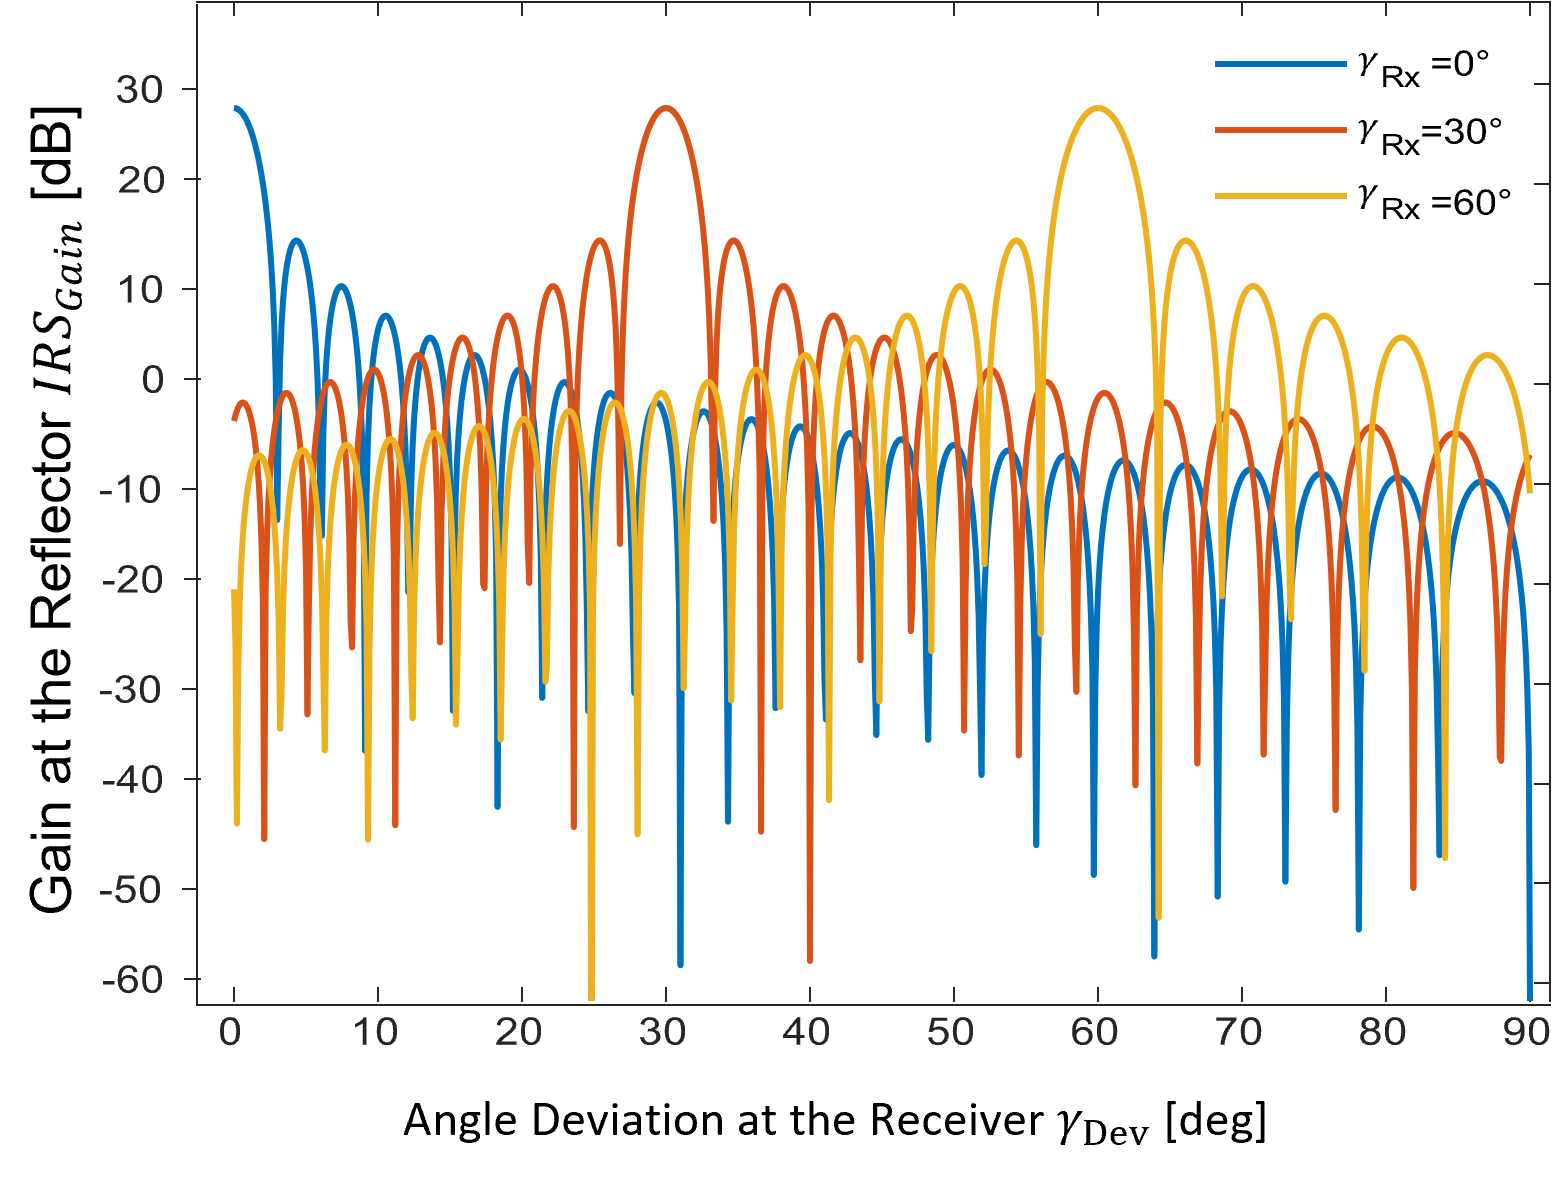
\includegraphics[width=0.7\linewidth]{images/Section 2 Images/model1_pattern}
	\caption{Gain at the reflector depicting the support of radiation pattern in \cite{8936989} when sweeping along the receiver i.e., $\gamma_{Rx} \neq \gamma_{Dev}$ for different placement of the receiver $\gamma_{Rx}$. A notable peak is observed for each $\gamma_{Rx}$ curve and the curve gradually decreases after this point. Additional parameters, $a=b=50\cdot \lambda$ at \SI{28}{\giga\hertz} frequency and $\theta_{Tx}=\varphi_{Tx}=0^\circ$. }
	\label{fig:model1pattern}
\end{figure}

All of these derivations of \ac{IRS} models are based on the Radar Cross Section which we discuss later in \Cref{Analytical Modeling of HELIOS Modules}. 
\section{Scope of Thesis} \label{Related Work or Scope of Thesis}
The previous sections have provided a thorough background on mmWave communications and particularly motivated the need for reflecting surfaces. Metasurfaces in the form of IRSs have risen as a hot topic in 6G research \cite{Scope_1, Scope_2, Scope_3, Scope_4}. Consequently, according end-to-end channel models have been developed.

As we have pointed out in this section, passive reflectors such as in the form of HELIOS reflectors are an alternative solution that comes with advantages in terms of compatibility with existing communication standards and zero-energy consumption. An analytical description for such is of utmost importance to realize HELIOS-enabled mmWave communications. Likewise, the goal of this master thesis is to derive such a description and compare it with the above IRS models. Similar to existing works, we aim to showcase the benefits of this model, particularly by using it in the context of an urban sample mmWave deployment scenario. 
				\chapter{Simulation and Analytical Modeling of HELIOS Reflectors} \label{Simulation and Analytical Modeling of HELIOS Reflectors}
This section develops an analytical model for the reflection behavior of HELIOS reflectors that are co-designed/validated via numerous EM simulations. First, we introduce the methodology of this in \Cref{sec:Simulation Methodology}. After laying the groundwork, \Cref{Simulative Analyses of HELIOS Reflector Modules} studies key reflection characteristics of HELIOS reflectors using an EM simulator.  Thereafter, \Cref{Analytical Modeling of HELIOS Modules} develops an analytical model for the reflection of individual HELIOS modules by building upon an existing radar cross-section formulae for flat plates and extending it according to the prior simulation results. Lastly, \Cref{Simulation and Modeling of HELIOS Reflectors} extends the analytical model to HELIOS reflectors to make up an array of individually parameterized modules. The thesis would focus on considering the self-shadowing effects that may occur between neighboring modules.
\section{Methodology}\label{sec:Simulation Methodology}
It is crucial to recognize that HELIOS is made up of a collection of HELIOS modules that all follow the same geometry template \cite{Helios}. However, the study draws attention to the unique feature that these modules may have different $\alpha$ and $\beta$ slopes. The corresponding paragraphs of \Cref{Passive reflectors} provide a more thorough explanation of this deviation from uniformity, highlighting the importance of these subtle adjustments to the overall structure and functionality of the HELIOS array. Using the author's definition in \cite{Helios}, we have constructed and integrated the geometry in the Ansys HFSS software which is a commercial EM simulation tool. We use the simulator as the fundamental physical prediction of the exhibited HELIOS reflection pattern which is strongly dependent on the geometry but also the angles of arrival of the incident EM wave.

The analytical modeling of the reflection behavior of arbitrarily configured HELIOS reflectors in \Cref{Analytical Modeling of HELIOS Modules}, and \Cref{Simulation and Modeling of HELIOS Reflectors} relies heavily on these simulative insights, particularly our initial detailed simulation study in \Cref{Simulative Analyses of HELIOS Reflector Modules}. Owing to this, we now outline the simulation workflow being used to attain the results presented in the forthcoming sections. We note that other commercial EM simulation tools offer the same functionality and should therefore operate similarly.

\Cref{fig:SimulationFlow} sketches the parametrization of the EM simulations of the HELIOS reflectors, thus providing a methodical and data-driven approach to investigate how key performance metrics, extractable from the simulation results for the specified far-field observation range, depending on the reflector configuration. In the above figure, an external IronPython script is used to automate the simulations in this case, which provides the simulation configuration in terms of the parametrization of the HELIOS reflector configuration under test as well as the scenario in terms of the incident wave, reflection observation angle range, and operating frequency. Here, the frequency is typically \SI{28}{\giga\hertz}, which lies in the 5G n\num{257} mmWave frequency band. The saved results are then analyzed using the MathWorks MATLAB tool to draw sensible conclusions. This knowledge shall then be used during the development of the analytical model in \Cref{Analytical Modeling of HELIOS Modules}, and \Cref{Simulation and Modeling of HELIOS Reflectors}.

\begin{figure}[tb]
	\centering
	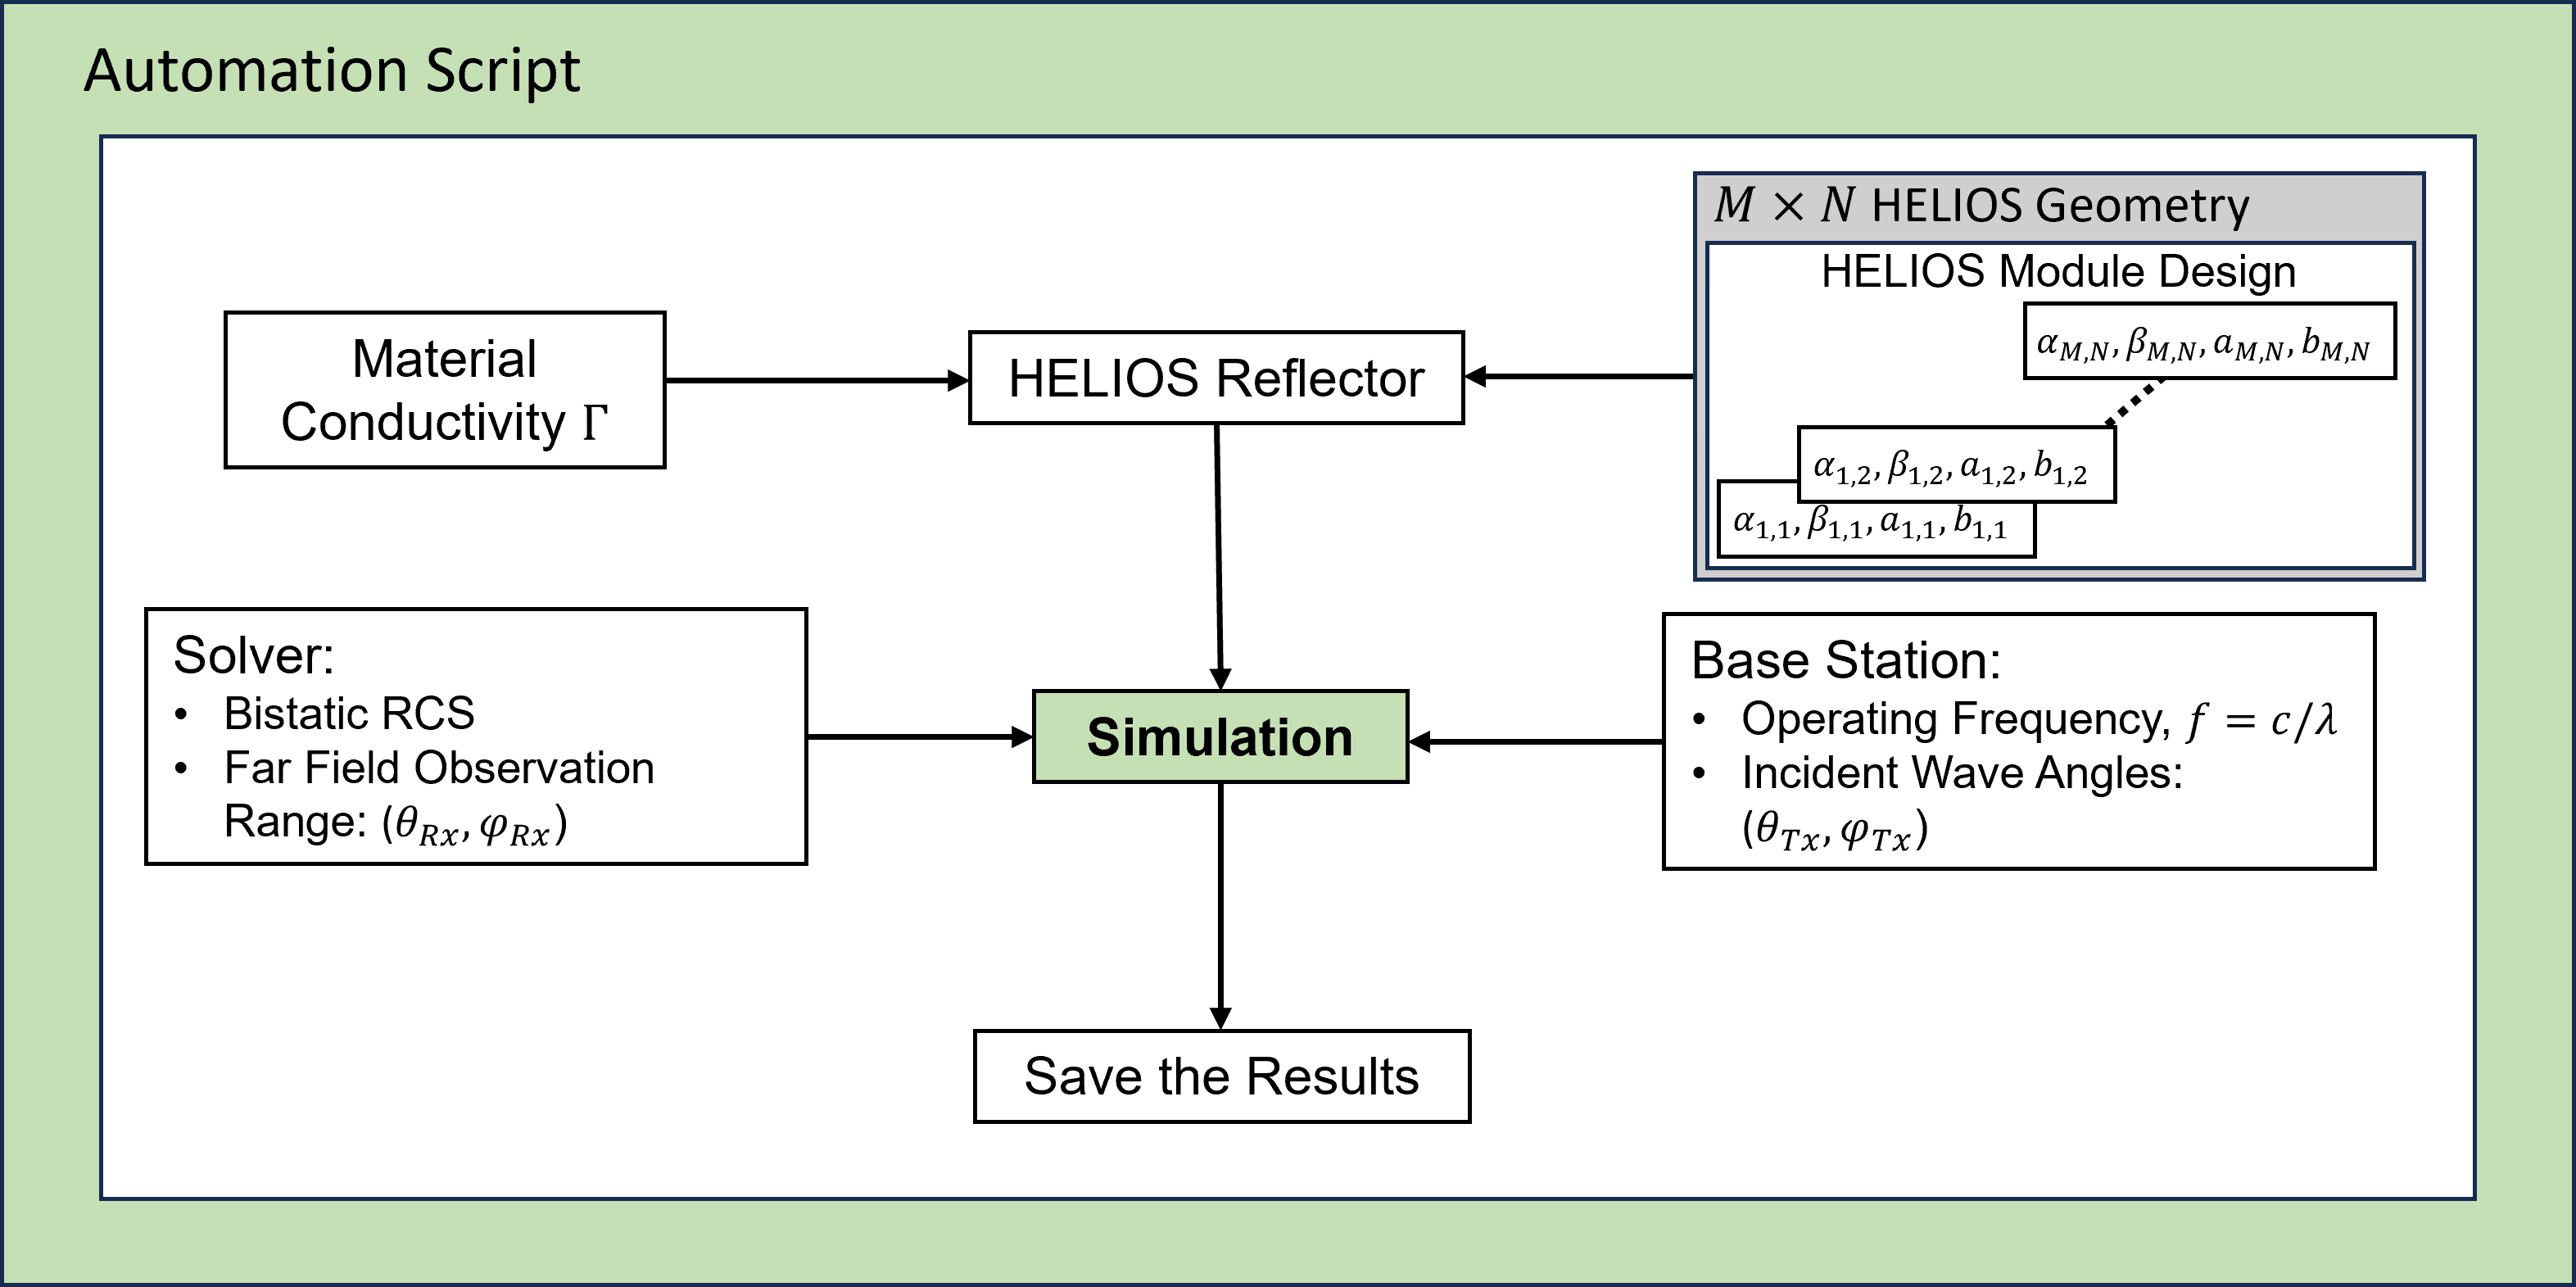
\includegraphics[width=1.0\linewidth]{images/Section 3 Images/Ansys_workflow}
	\caption{Illustration of the EM simulation workflow of the HELIOS reflectors. Simulation parameters in terms of base station configuration, far-field settings, and HELIOS reflector may be changed as desired for each simulation using an automation script.}
	\label{fig:SimulationFlow}
\end{figure}
Horizontal and vertical angles of incidence as well as of departure will all adhere to $\varphi_{Tx}, \theta_{Tx} \in [-90, 90]^\circ$ using the coordinate system defined in \Cref{coordinate systems}. These angles of incidence will be varied in this study to consider different deployment scenarios. The far-field observation range typically constitutes the half-sphere spanned by the above-defined range. Due to the simulation complexity, the resolution of simulation for this set of angles differs depending on, e.g., the HELIOS reflector size. For each of these points along the half-sphere, the EM simulator calculates the bistatic RCS (see \Cref{Analytical Modeling of HELIOS Modules}).

As discussed before, each HELIOS reflector element $\left(m,n\right)$ consists of four crucial parameters, i.e., dimensions $a_{m,n}$, and $b_{m,n}$ being the footprint sizes along $y$ and $z$-axes, respectively, and slopes $\alpha_{m,n}$, and $\beta_{m,n}$ constituting the horizontal and vertical slopes, respectively. The whole HELIOS reflector consists of $M \times N$ elements with $m\in1,\dots,M$ and $n \in 1, \dots, N$, cf. \Cref{Metasurfaces}. In this work, we assume that all individual elements have the same footprints, i.e., $a=a_{m,n}\in m,n$ and $b=b_{m,n} \in m, n$. Therefore, there are $2 \cdot N \cdot M + 2$ parameters constituting a HELIOS geometry. In the scope of \Cref{Simulative Analyses of HELIOS Reflector Modules}, the impact of selecting different common materials will be tested. In addition, artificial materials with arbitrary conductivity will be studied. Thereafter, copper will be used as the HELIOS baseline material as in \cite{Helios}.
The term "Gain" refers to the RCS, as elucidated in \Cref{Analytical Modeling of HELIOS Modules}, throughout this work. This application of the term gain is consistent with the definition given in \Cref{coordinate systems}, which presents a direct comparison of all three IRS models. A cohesive and seamless interpretation of the RCS behavior across different model comparisons is ensured by the study's maintenance of terminology compatibility.
\section{Simulative Analyses of HELIOS Reflector Modules} \label{Simulative Analyses of HELIOS Reflector Modules}
In this section, we thoroughly assess the reflection characteristics of a single-element HELIOS reflector to shed light on how it behaves for various parameter combinations. This section is divided into three sections, each of which focuses on a different component of the evaluation. The study looks into the effects of changing slope angles in \Cref{Variation of Slope Angle} to comprehend how these changes affect the system as a whole. In \Cref{Variation of Element Size}, the impacts of different reflector sizes are examined to determine how size variations affect the system's performance. In conclusion, \Cref{Impact of Material Conductivity} delves into the effects of altering the materials that make up the reflecting surface, thereby offering a comprehensive understanding of how distinct materials influence the overall performance and effectiveness of the reflective system.
%\begin{itemize}
%	\item \textbf{Variation concerning Slope Angle \textbf{$\alpha$}}
%	\item \textbf{Reflector Length Variation}
%	\item \textbf{Material Variations}
%\end{itemize}
%\begin{figure}
%	\centering
%	
\includegraphics[width=1.0\linewidth]{images/Section 3 Images/orientations4}
%	\caption{Depicting the four variations of real-time implementations in orientations of a HELIOS module.}
%	\label{fig:orientations4}
%\end{figure}
\subsection{Variation of Slope Angle} \label{Variation of Slope Angle}
Using the fundamental HELIOS idea as a starting point, a significant departure from the established law of reflection i.e., $\varphi_{Rx} \neq -\varphi_{Tx}$ and $\theta_{Rx} \neq -\theta_{Tx}$ appears. \Cref{fig:HELIOS-model} shows the design of the HELIOS reflectors with the size of the reflectors $a$ and $b$ as well as the slope angles $\alpha$ and $\beta$, which are intricately related to the dimensions of the reflecting surface. The model here assumes that have incident wave is orthogonal to the reflector module base ($\theta_{Tx}=\varphi_{Tx}=0^\circ$). As presented by the authors in \cite{Helios}, this results in a noticeable change in the reflected angle by two times the slope angle, see \Cref{HELIOS 2times beta} and \Cref{HELIOS 2times alpha} below.
\begin{figure}[tb]
	\centering
	\includegraphics[width=0.7\linewidth]{images/Section 3 Images/HELIOS model}
	\caption{HELIOS module with the implementation of $\alpha$ and $\beta$ slope angles with incident wave orthogonal to the reflector base i.e., $\theta_{Tx}=\varphi_{Tx}=0^\circ$ and reflected wave validating HELIOS concept \cite{Helios} with two times shift in the slope angles.}
	\label{fig:HELIOS-model}
\end{figure}
\begin{equation} \label{HELIOS 2times beta}
	\theta_{Rx}=-\theta_{Tx}+2 \cdot \beta \\
\end{equation}
\begin{equation} \label{HELIOS 2times alpha}
	\varphi_{Rx}=-\varphi_{Tx}+2 \cdot \alpha \\
\end{equation}
In our first simulative study, we focus on the variation of the horizontal slope angle $\alpha$ within the range of $[\num{0}:\num{80}]^\circ$, in our effort to comprehend the complex dynamics of our HELIOS reflector modules. This investigation is essential in figuring out how slope angles affect the behavior of the model. Let us consider a simplified scenario where vertical slope angle $\beta=\num{0}^\circ$ is held constant to validate these intriguing results and the variation in $\varphi_{Rx}$ as a function of $\alpha$ to best illustrate the essence of this experiment (see \Cref{fig:saturation}). Notably, within the range of $\alpha$ from $\num{0}^\circ$ to $\num{45}^\circ$, \Cref{HELIOS 2times beta} and \Cref{HELIOS 2times alpha} accurately capture the behavior of the model. Beyond the $\num{45}^\circ$ threshold of $\alpha$, something different happens because the term $2 \cdot \alpha$ exceeds $\num{90}^\circ$.

This behavior as shown in \Cref{fig:saturation}, causes the beams to go beyond the limits of the considered far-field, resulting in a seeming saturation effect. The reason for this behavior is the energy being reflected behind the reflector which can be seen on the right side of the figure \Cref{fig:saturation}. As such, these results show that HELIOS modules can indeed direct the reflection into a target direction by setting
$\alpha = (\varphi_{Rx}+\varphi_{Tx})/2$ and $\beta = (\theta_{Rx}+\theta_{Tx})/2$.
\begin{figure}[H]
	\centering
	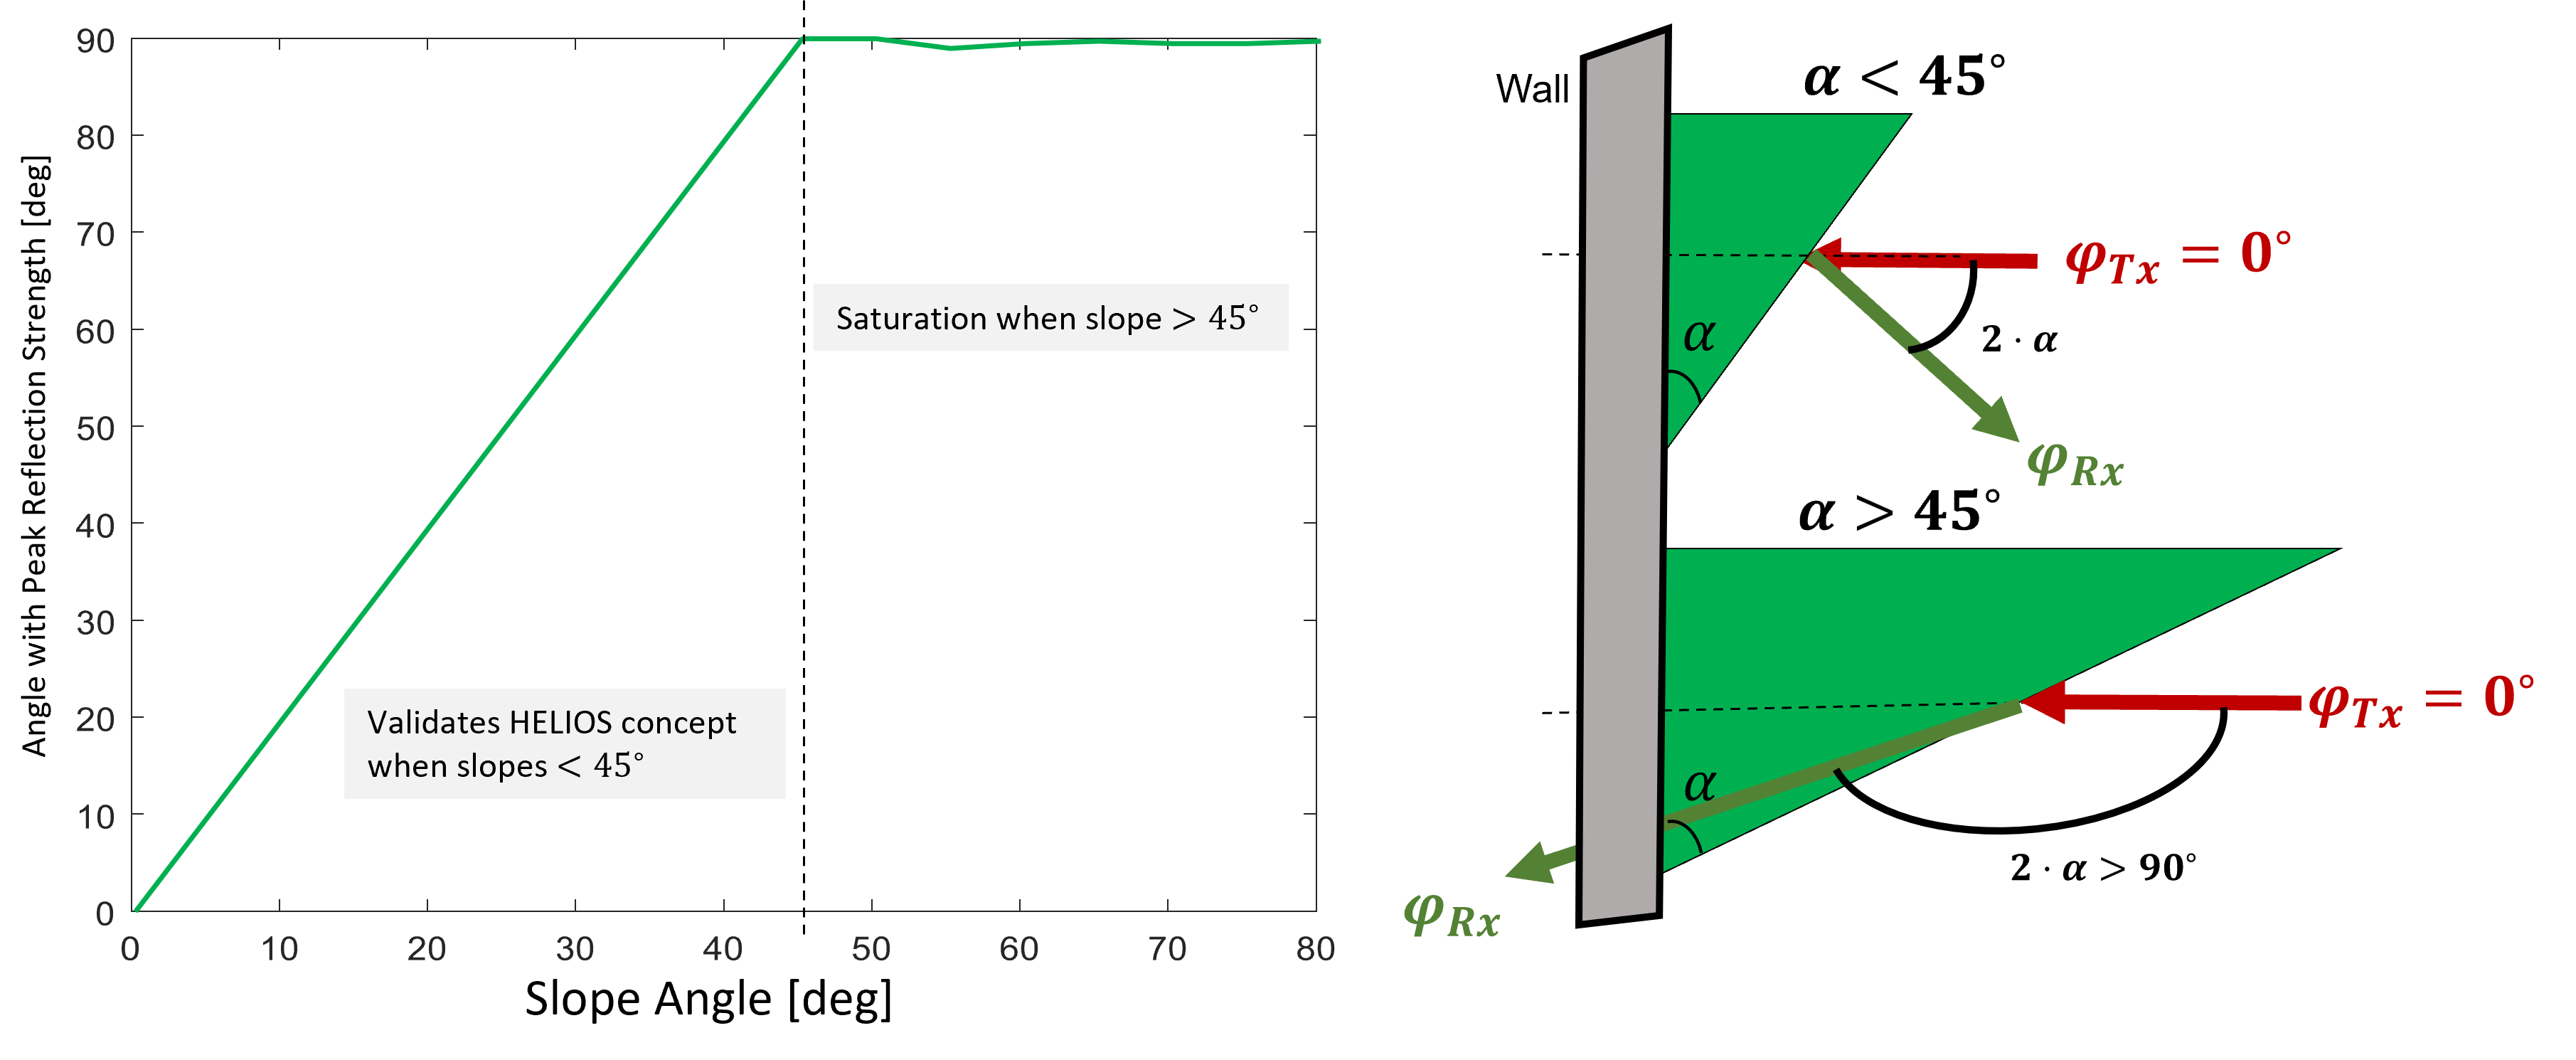
\includegraphics[width=0.93\linewidth]{images/Section 3 Images/Saturation}
	\caption{Assessment of the peak reflection angle given $\varphi_{Tx}=\theta_{Tx}=0^\circ$ and different module slopes. We observe that reflection angle $\varphi_{Rx} = -\varphi_{Tx} + 2\cdot \alpha$ and we note that the saturation for slopes $< \num{45}^\circ$ is misleading as this depends on the angle of arrival of the incident wave and, in particular, is caused by the maximum reflection angle being outside the specified observation angle range for the simulation. This is because the energy is reflected behind the reflector as sketched on the right side.}
	\label{fig:saturation}
\end{figure}
\subsection{Effect of Different Reflector Sizes} \label{Variation of Element Size}
We now make a complementary investigation of the impact of the HELIOS element footprint dimensions $a$ and $b$ with $a=b$ in the range from \num{1} to \SI{90}{\centi\meter}.

\begin{figure}[tb]
	\centering
	\subfloat[Azimuth angle variation at the reflector for various reflector sizes, plotted against gain in \si{\decibel} at \SI{28}{\giga\hertz} frequency with slope angle $\alpha=\num{22.5}^\circ$ with $\theta_{Rx}=0^\circ$. Notably, the beams become narrower as the reflector size increases.]{
	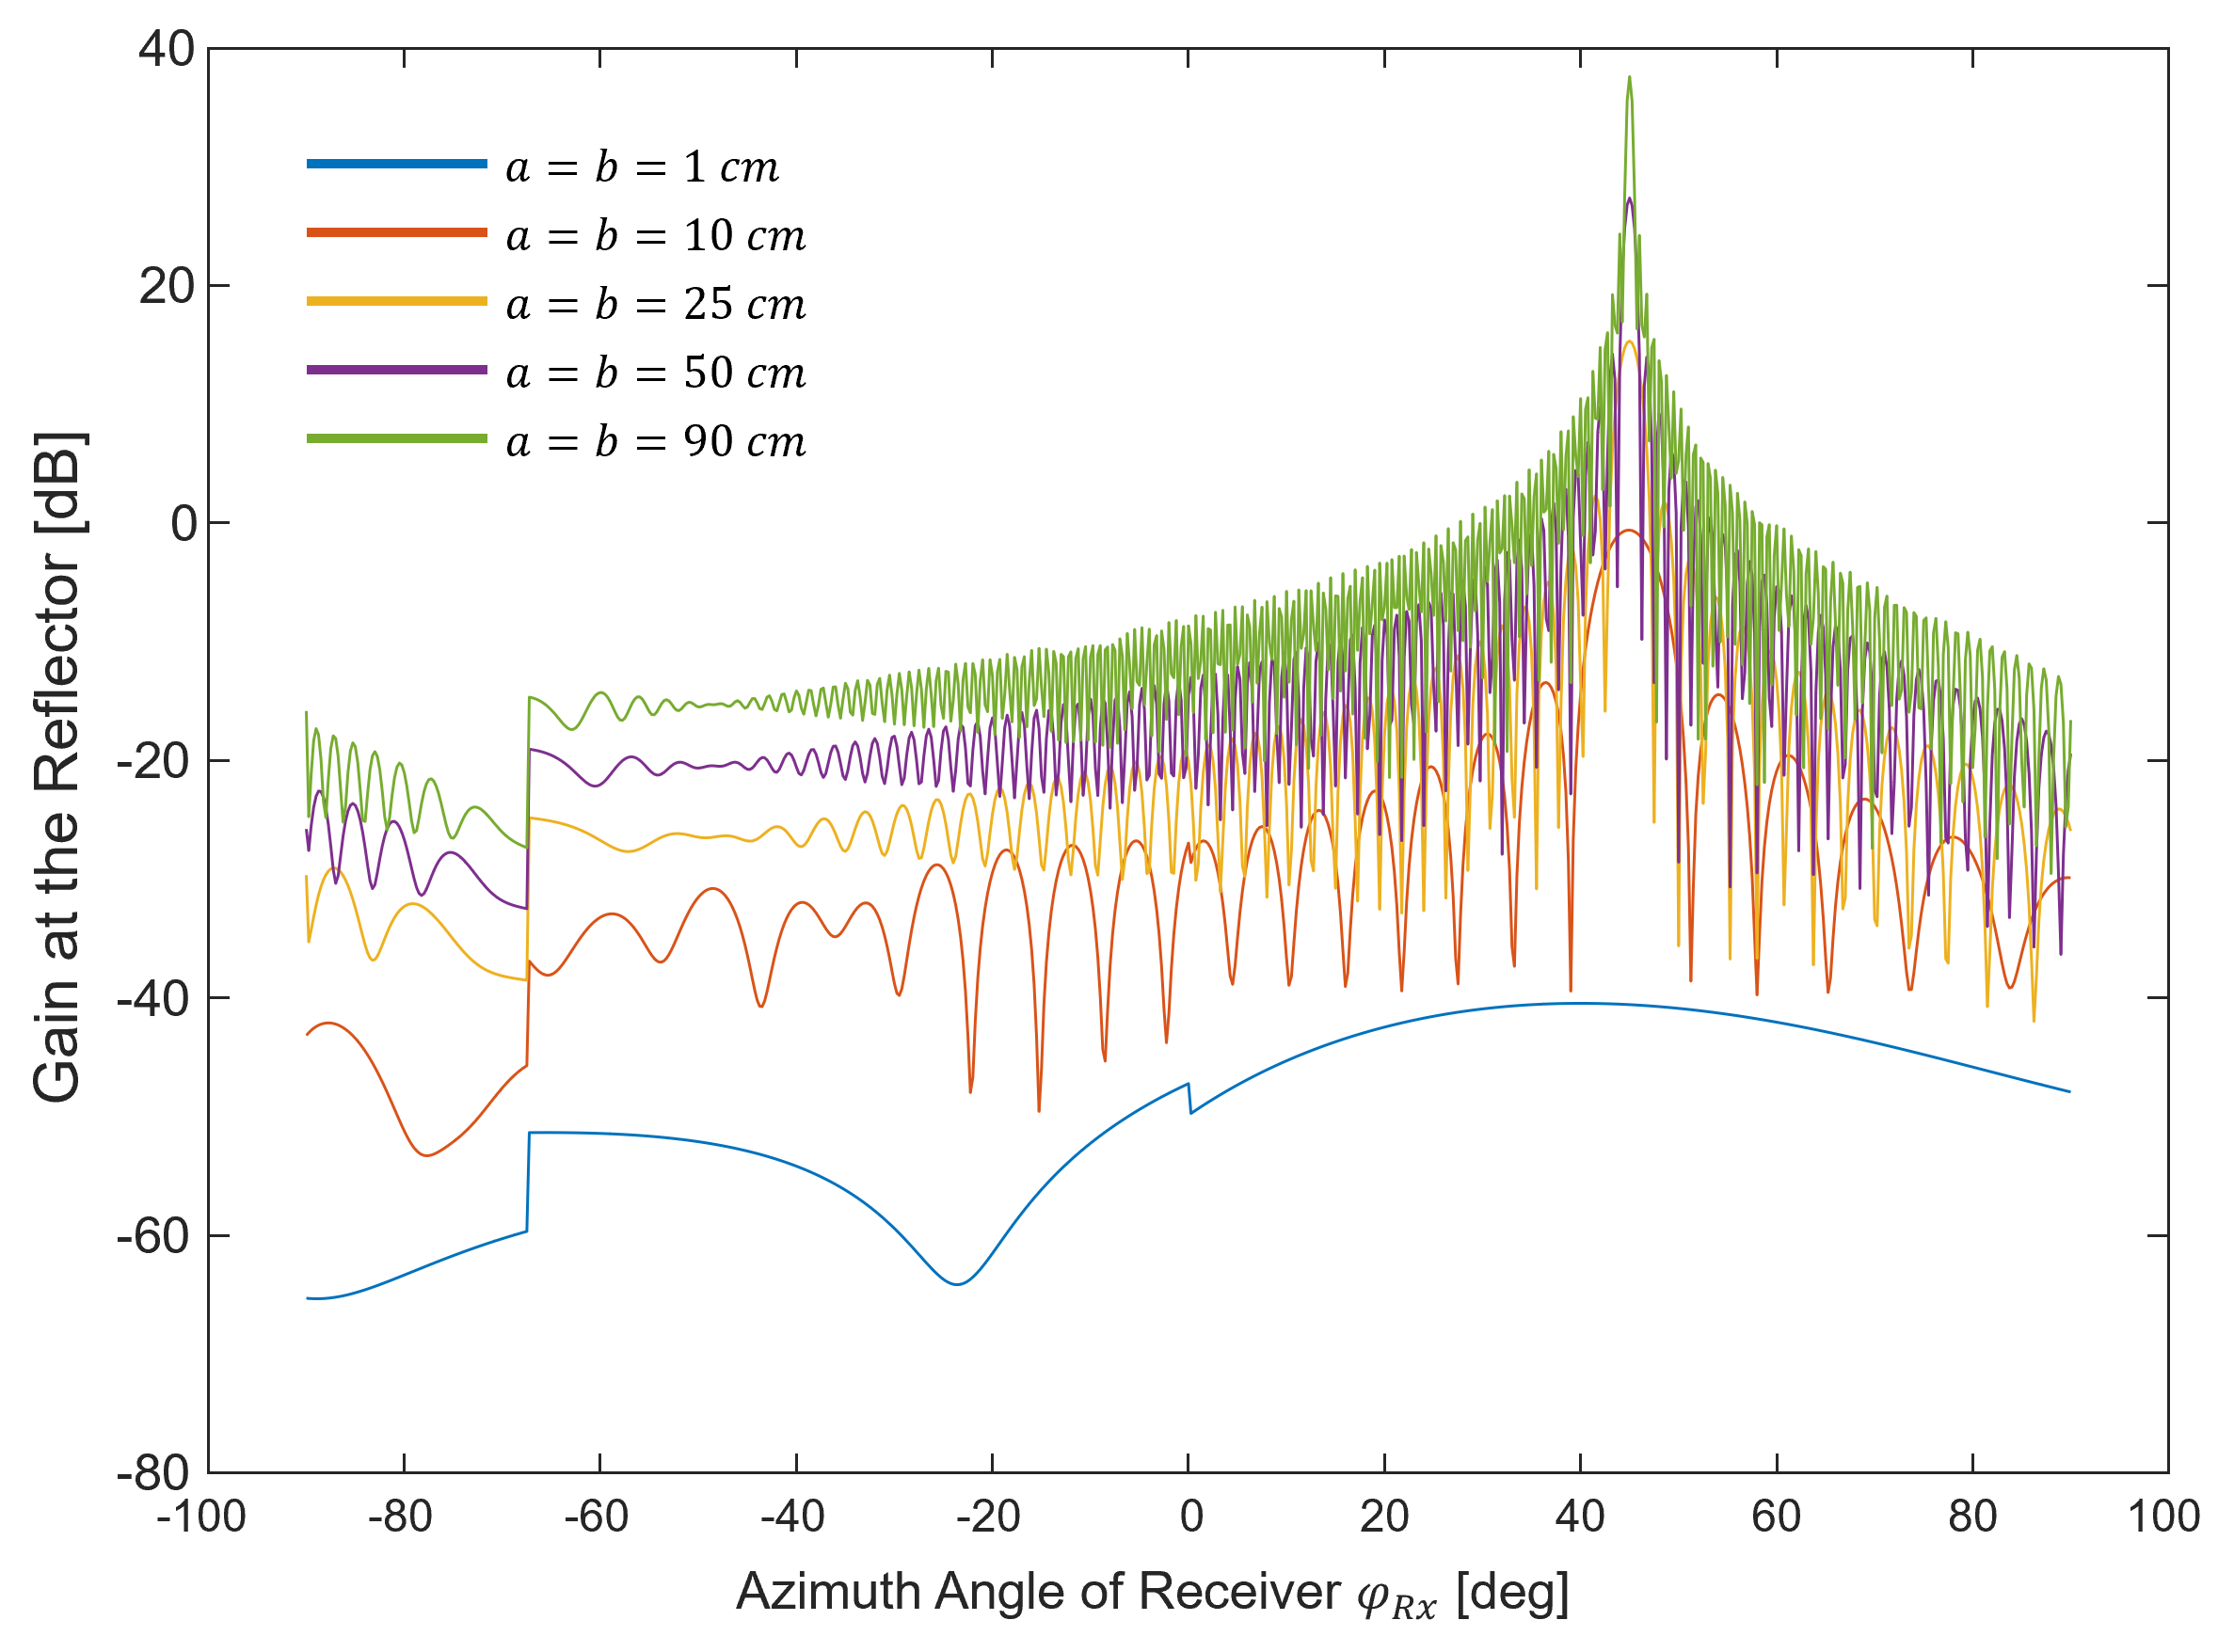
\includegraphics[width=0.5\linewidth]{images/Section 3 Images/Reflector_length_2}
		\label{fig:rl3}
	}
	\hfill
	\subfloat[Behavior of HELIOS module for varying reflector size $a$ and $b$ when plotted against peak gain in \si{\decibel}. A notable increase in gain by \SI{12}{\decibel} is observed when the reflector size is doubled.]{
	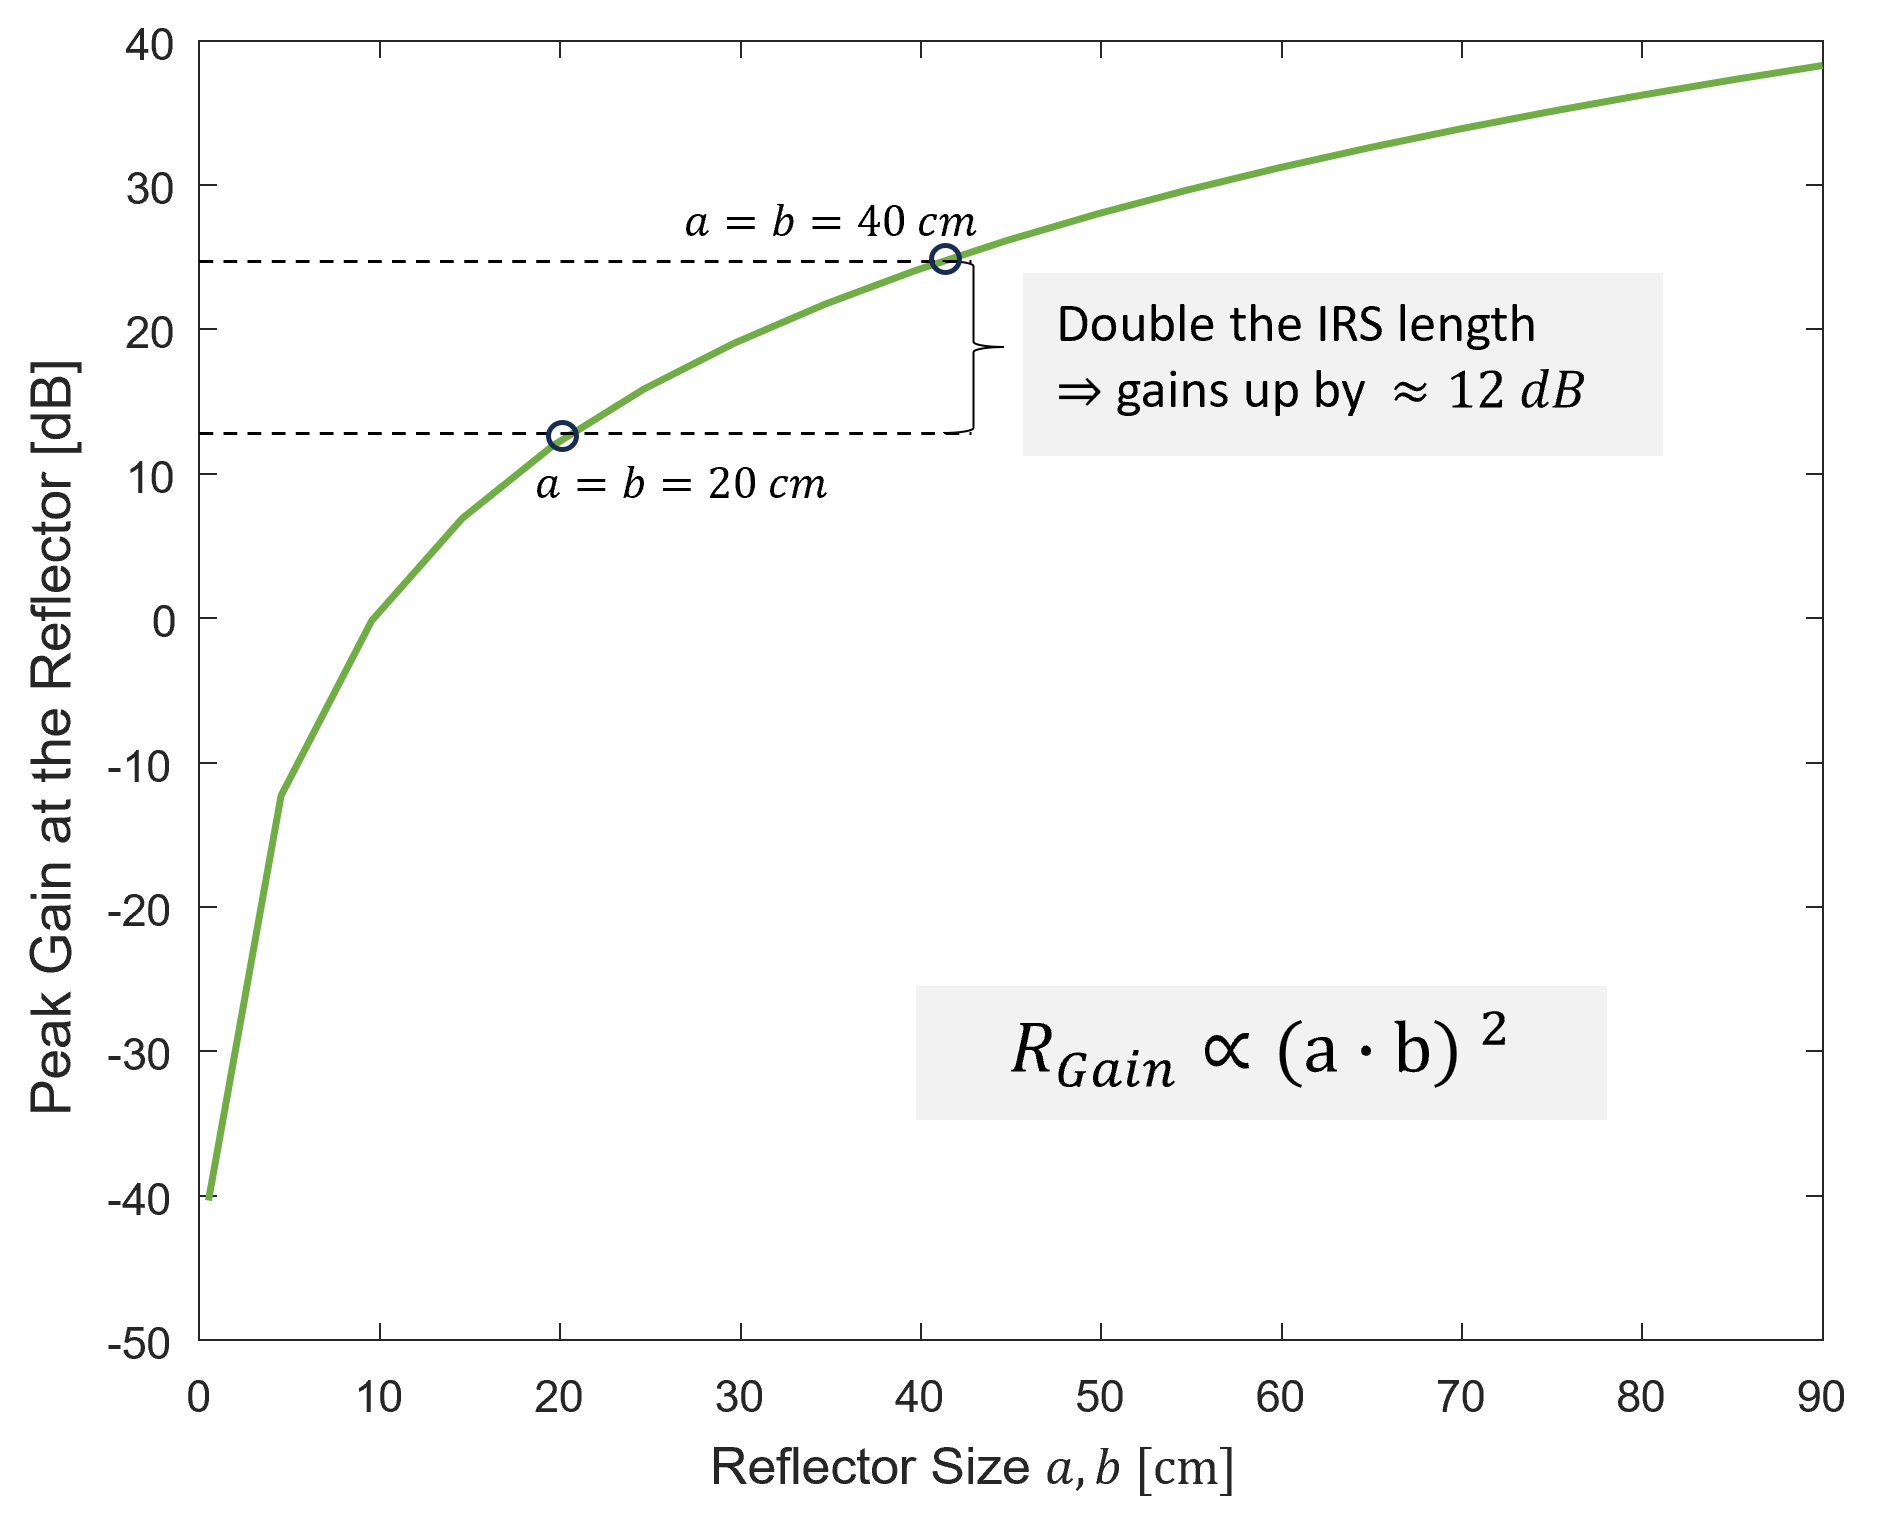
\includegraphics[width=0.45\linewidth]{images/Section 3 Images/Reflector_length}
		\label{fig:rl1}
	}
	\caption[Illustration of the impact of the variations in reflector sizes of HELIOS module on the beam pattern and peak gain at the reflector as the size increases.]{Illustration of the impact of the variations in reflector sizes of HELIOS module on the beam pattern and peak gain at the reflector as the size increases.}
	\label{}
\end{figure}
%\begin{figure}[H]
%	\centering
%	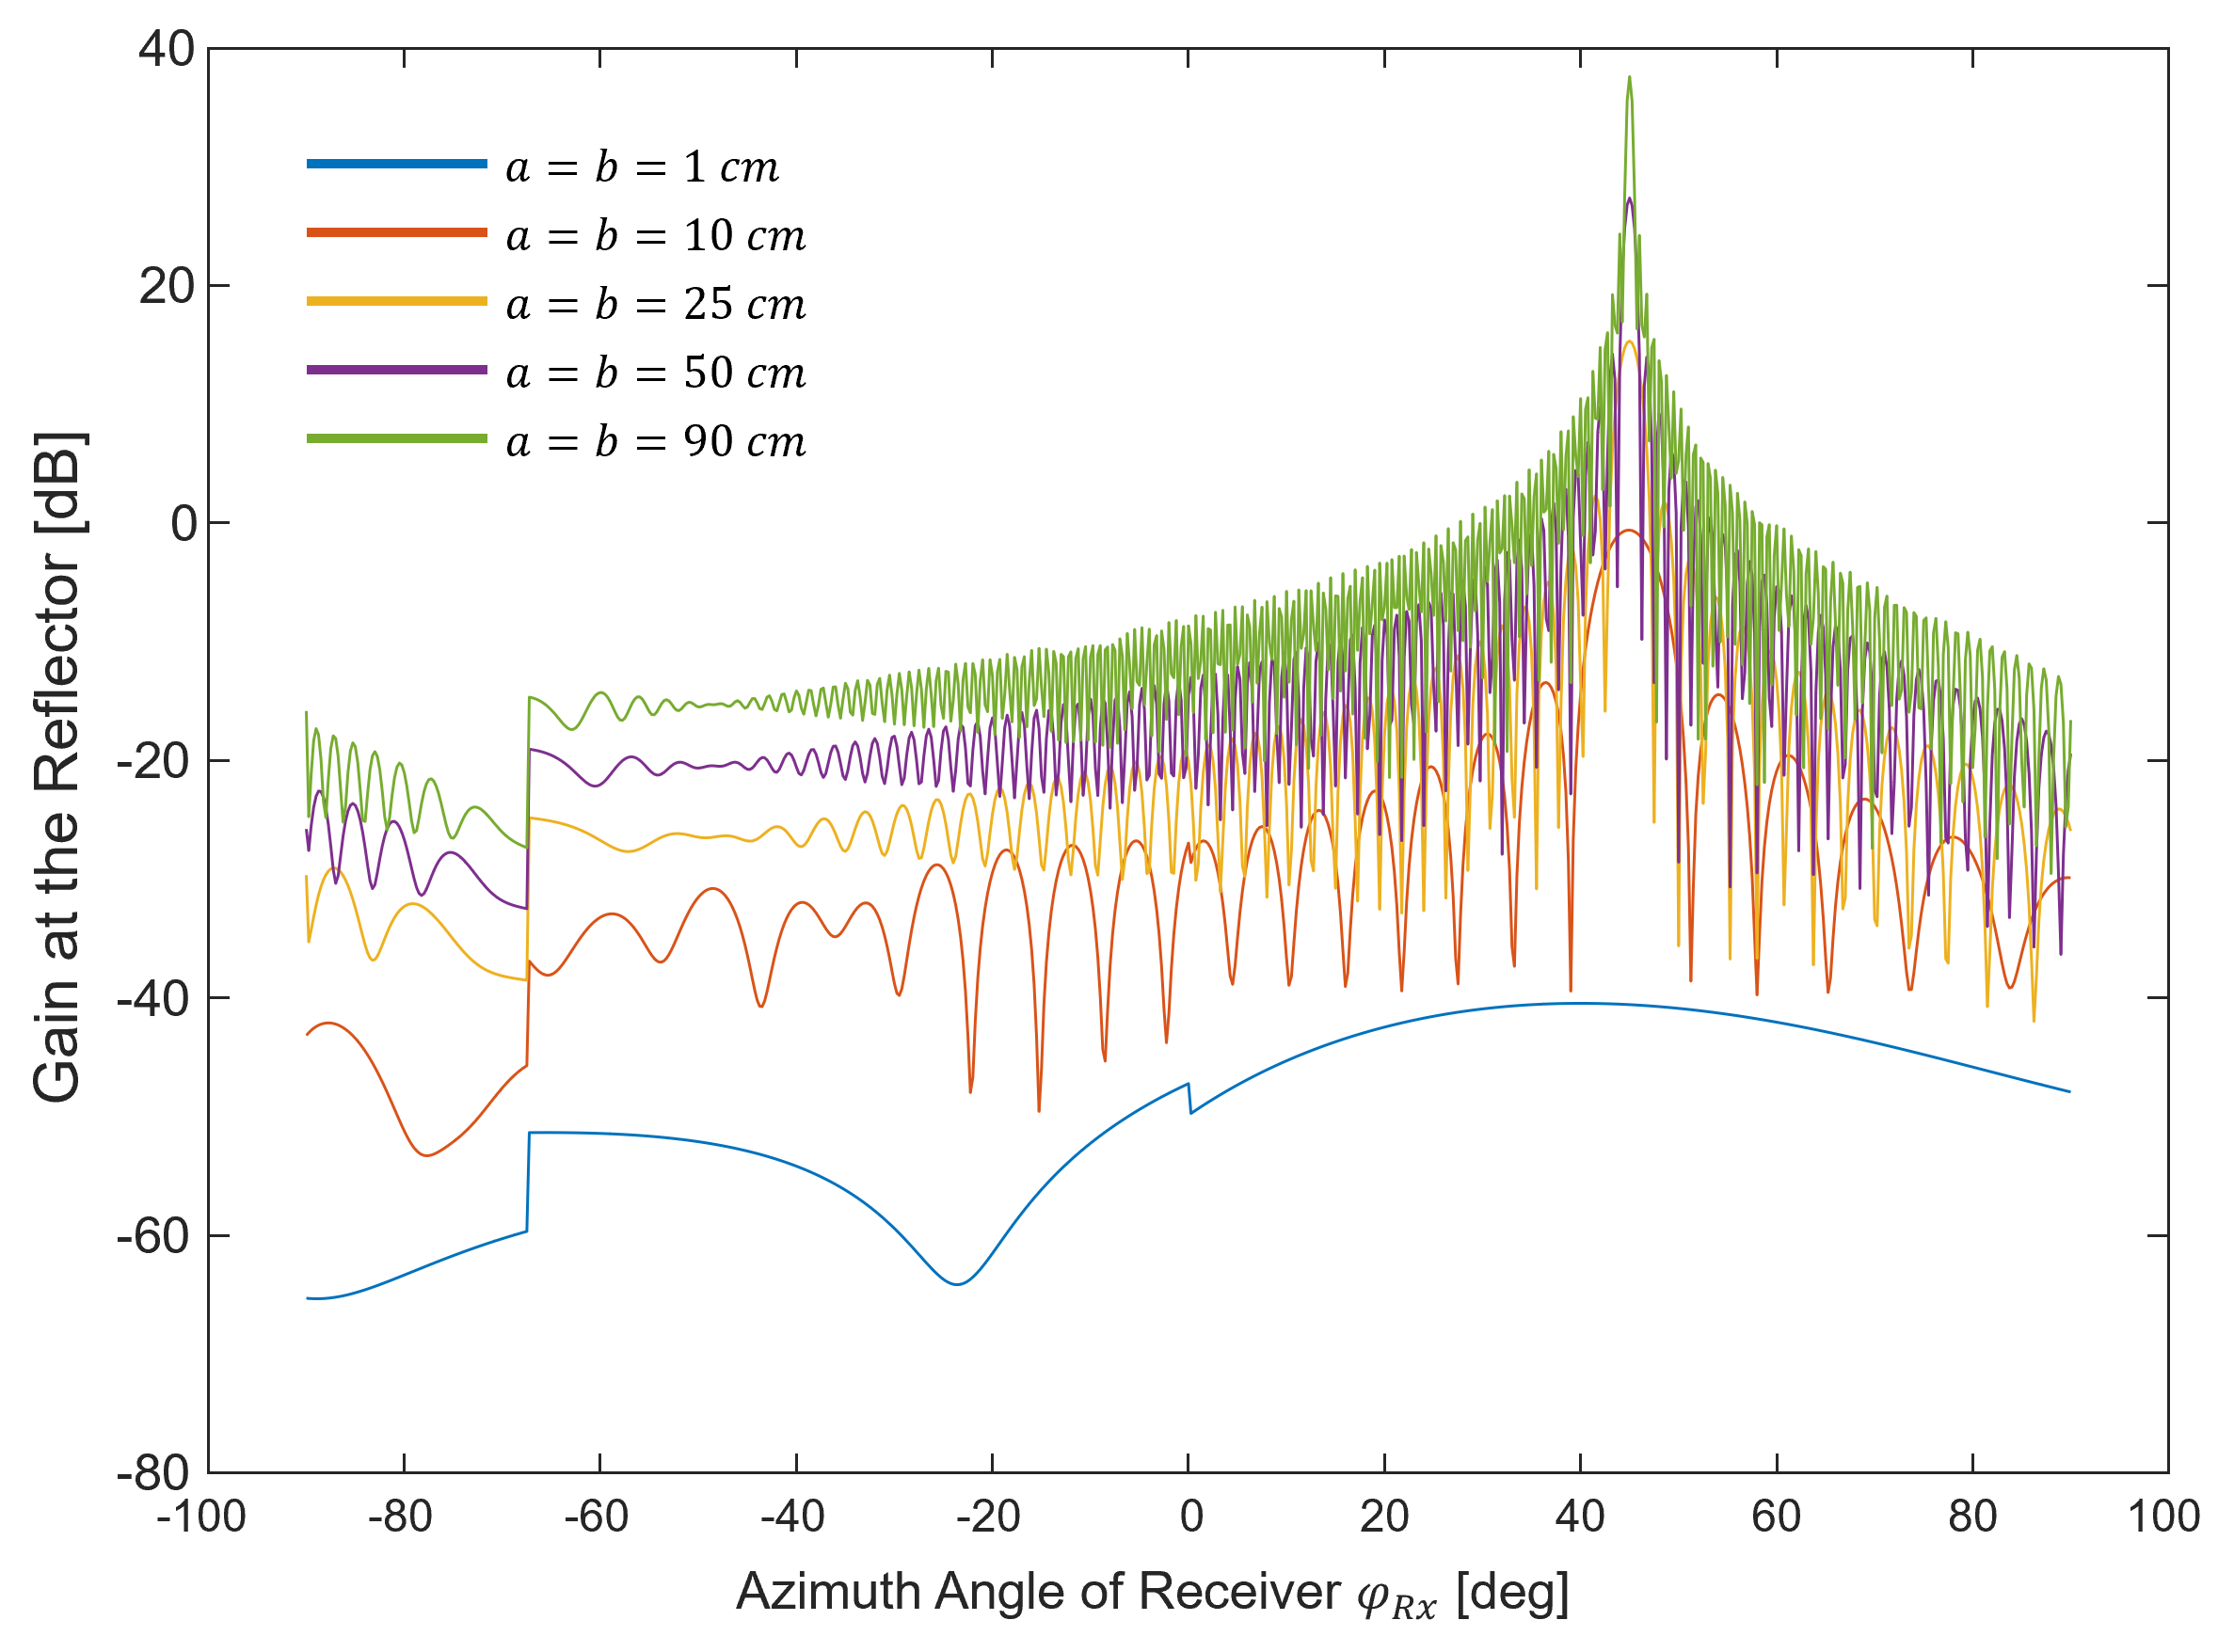
\includegraphics[width=0.8\linewidth]{images/Section 3 Images/Reflector_length_2}
%	\caption{Azimuth angle variation at the reflector for various reflector sizes, plotted against gain in \si{\decibel}.}
%	\label{fig:rl3}
%\end{figure}
%\begin{figure}[H]
%	\centering
%	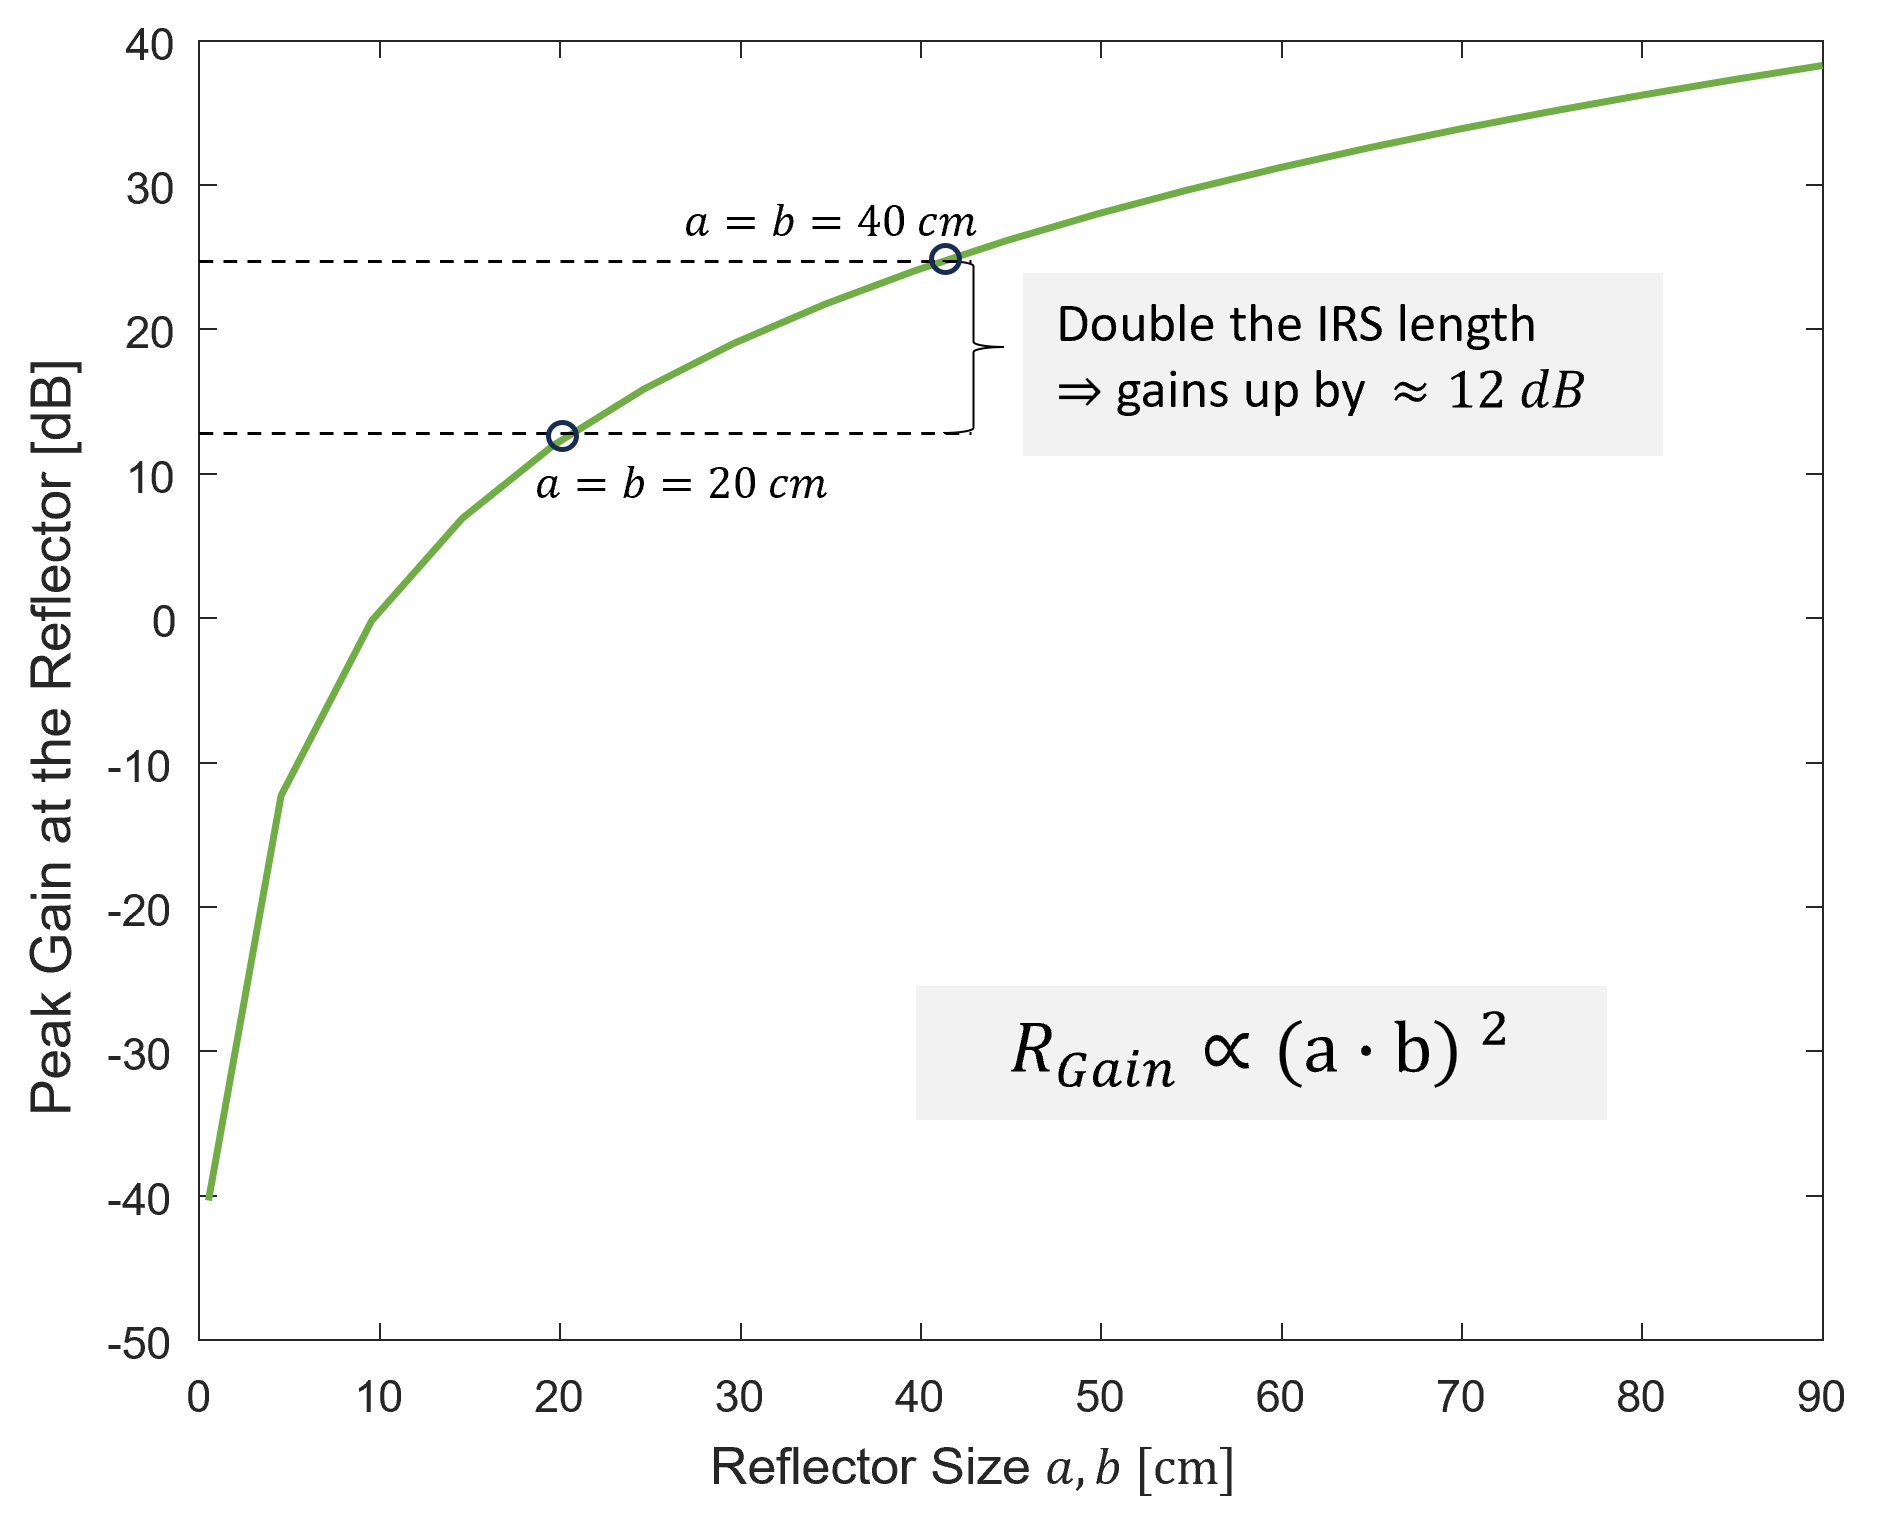
\includegraphics[width=1.0\linewidth]{images/Section 3 Images/Reflector_length}
%	\caption{Behavior of HELIOS module for varying reflector size when plotted against gain in \si{\decibel} for different orientations. Linear scale behavior of HELIOS module for varying reflector size which validates the gain proportionality with reflector dimensions.}
%	\label{fig:rl1}
%\end{figure}
The simulation results in \Cref{fig:rl3} illustrate that larger reflecting surfaces produce a higher gain. Moreover, with increasing size, the main lobe also becomes more narrow such that energy is reflected in a more concentrated fashion. The results in \Cref{fig:rl1} match the analytical modeling carried out in \Cref{coordinate systems} in regards to the maximal gain which scales with $(a\cdot b)^2$, cf. gain increase by \SI{40}{\decibel} when increasing the surface area by a \num{100} from $a=b=\SI{1}{\centi\meter}$ to $a=b=\SI{50}{\centi\meter}$. As observed from the same figure, as we double the size of the reflector from $a=b=\SI{20}{\centi\meter}$ to $a=b=\SI{40}{\centi\meter}$, the peak gain increases by almost \SI{12}{\decibel}. This result confirms that reflector size is a key metric to be tuned to attain the necessary power gains for mmWave beyond LOS connectivity.
\subsection{Impact of Reflecting Surface Material} \label{Impact of Material Conductivity}
Lastly, we study the impact of material properties on the reflection behavior. In the first part, we consider seven different real materials. Thereafter, we consider the impact of the material conductivity directly. 
\begin{table}[tb] % H -> dieses objekt wird genau da wo der code steht festgenagelt
			\caption{Properties of different materials in terms of conductivity and relative permittivity.}
		\footnotesize
	\label{Conductivity table}
	\centering
	\begin{tabular}{c|c|c}
		\textbf{Materials} & \textbf{Conductivity} (\si{\siemens/\meter}) & \textbf{Relative Permittivity} \\
		\hline
		Copper & 58,000,000 & 1 \\
		\hline
		FR4 & 0 & 4.4 \\
		\hline
		Glass & 0 & 5.5 \\
		\hline
		Perfect Electric Conductor & 1e+30 & 1 \\
		\hline
		Tantalum & 6,300,000 & 1 \\
		\hline
		Stainless Steel & 1,100,000 & 1 \\
		\hline
		Rubber & 0 & 3.0
	\end{tabular}
\end{table}
First, we consider the maximum gain by HELIOS modules based on the seven materials given in \Cref{Conductivity table}. The maximum gains observed in \Cref{fig:conductivity1} underline that high material conductivity results in stronger reflections. As a result, high gains can only be realized by using large reflecting surfaces (cf. \Cref{Variation of Element Size}) and correct slope angles (cf. \Cref{Variation of Slope Angle}) in combination with a suitable reflecting surface material such as copper. Since the four materials yielding high gains have very similar peak gains, we now do a sensitivity analysis for a wide range of conductivity values using an artificial material, copper, and only alter the conductivity parameter as needed.

The sweep range is between $\num{0}$ to 10,000 $\si{\siemens/\meter}$ and thus exceeds the conductivity of glass, FR4, and rubber by far. However, the value is much smaller than that of, e.g., copper. The findings, as shown in \Cref{fig:conductivity2}, underline that the reflection gain does indeed depend nearly linearly on the material conductivity, as underlined by the linear regression curve (red). This behavior matches the IRS model dependence on parameter $\Gamma$ in \Cref{coordinate systems}. 
 
The potential to use these materials to improve the performance of our HELIOS reflector modules in practical applications is highlighted by the intriguing consistency between the behavior of high conductivity materials and the IRS models. We are better able to design and deploy our modules for practical and efficient use if we are aware of these subtle interactions between materials and their conductivity values.

\begin{figure}[H]
	\centering
	\subfloat[Effect of different materials on HELIOS module when plotted against the gain in \si{\decibel}. Parameters: $\alpha=22.5^\circ$, $\beta=0^\circ$, $a=b= \num{50} \cdot \lambda$ with incident wave $\varphi_{Tx}=\theta_{Tx}=0^\circ$ at \SI{28}{\giga\hertz} frequency.]{
		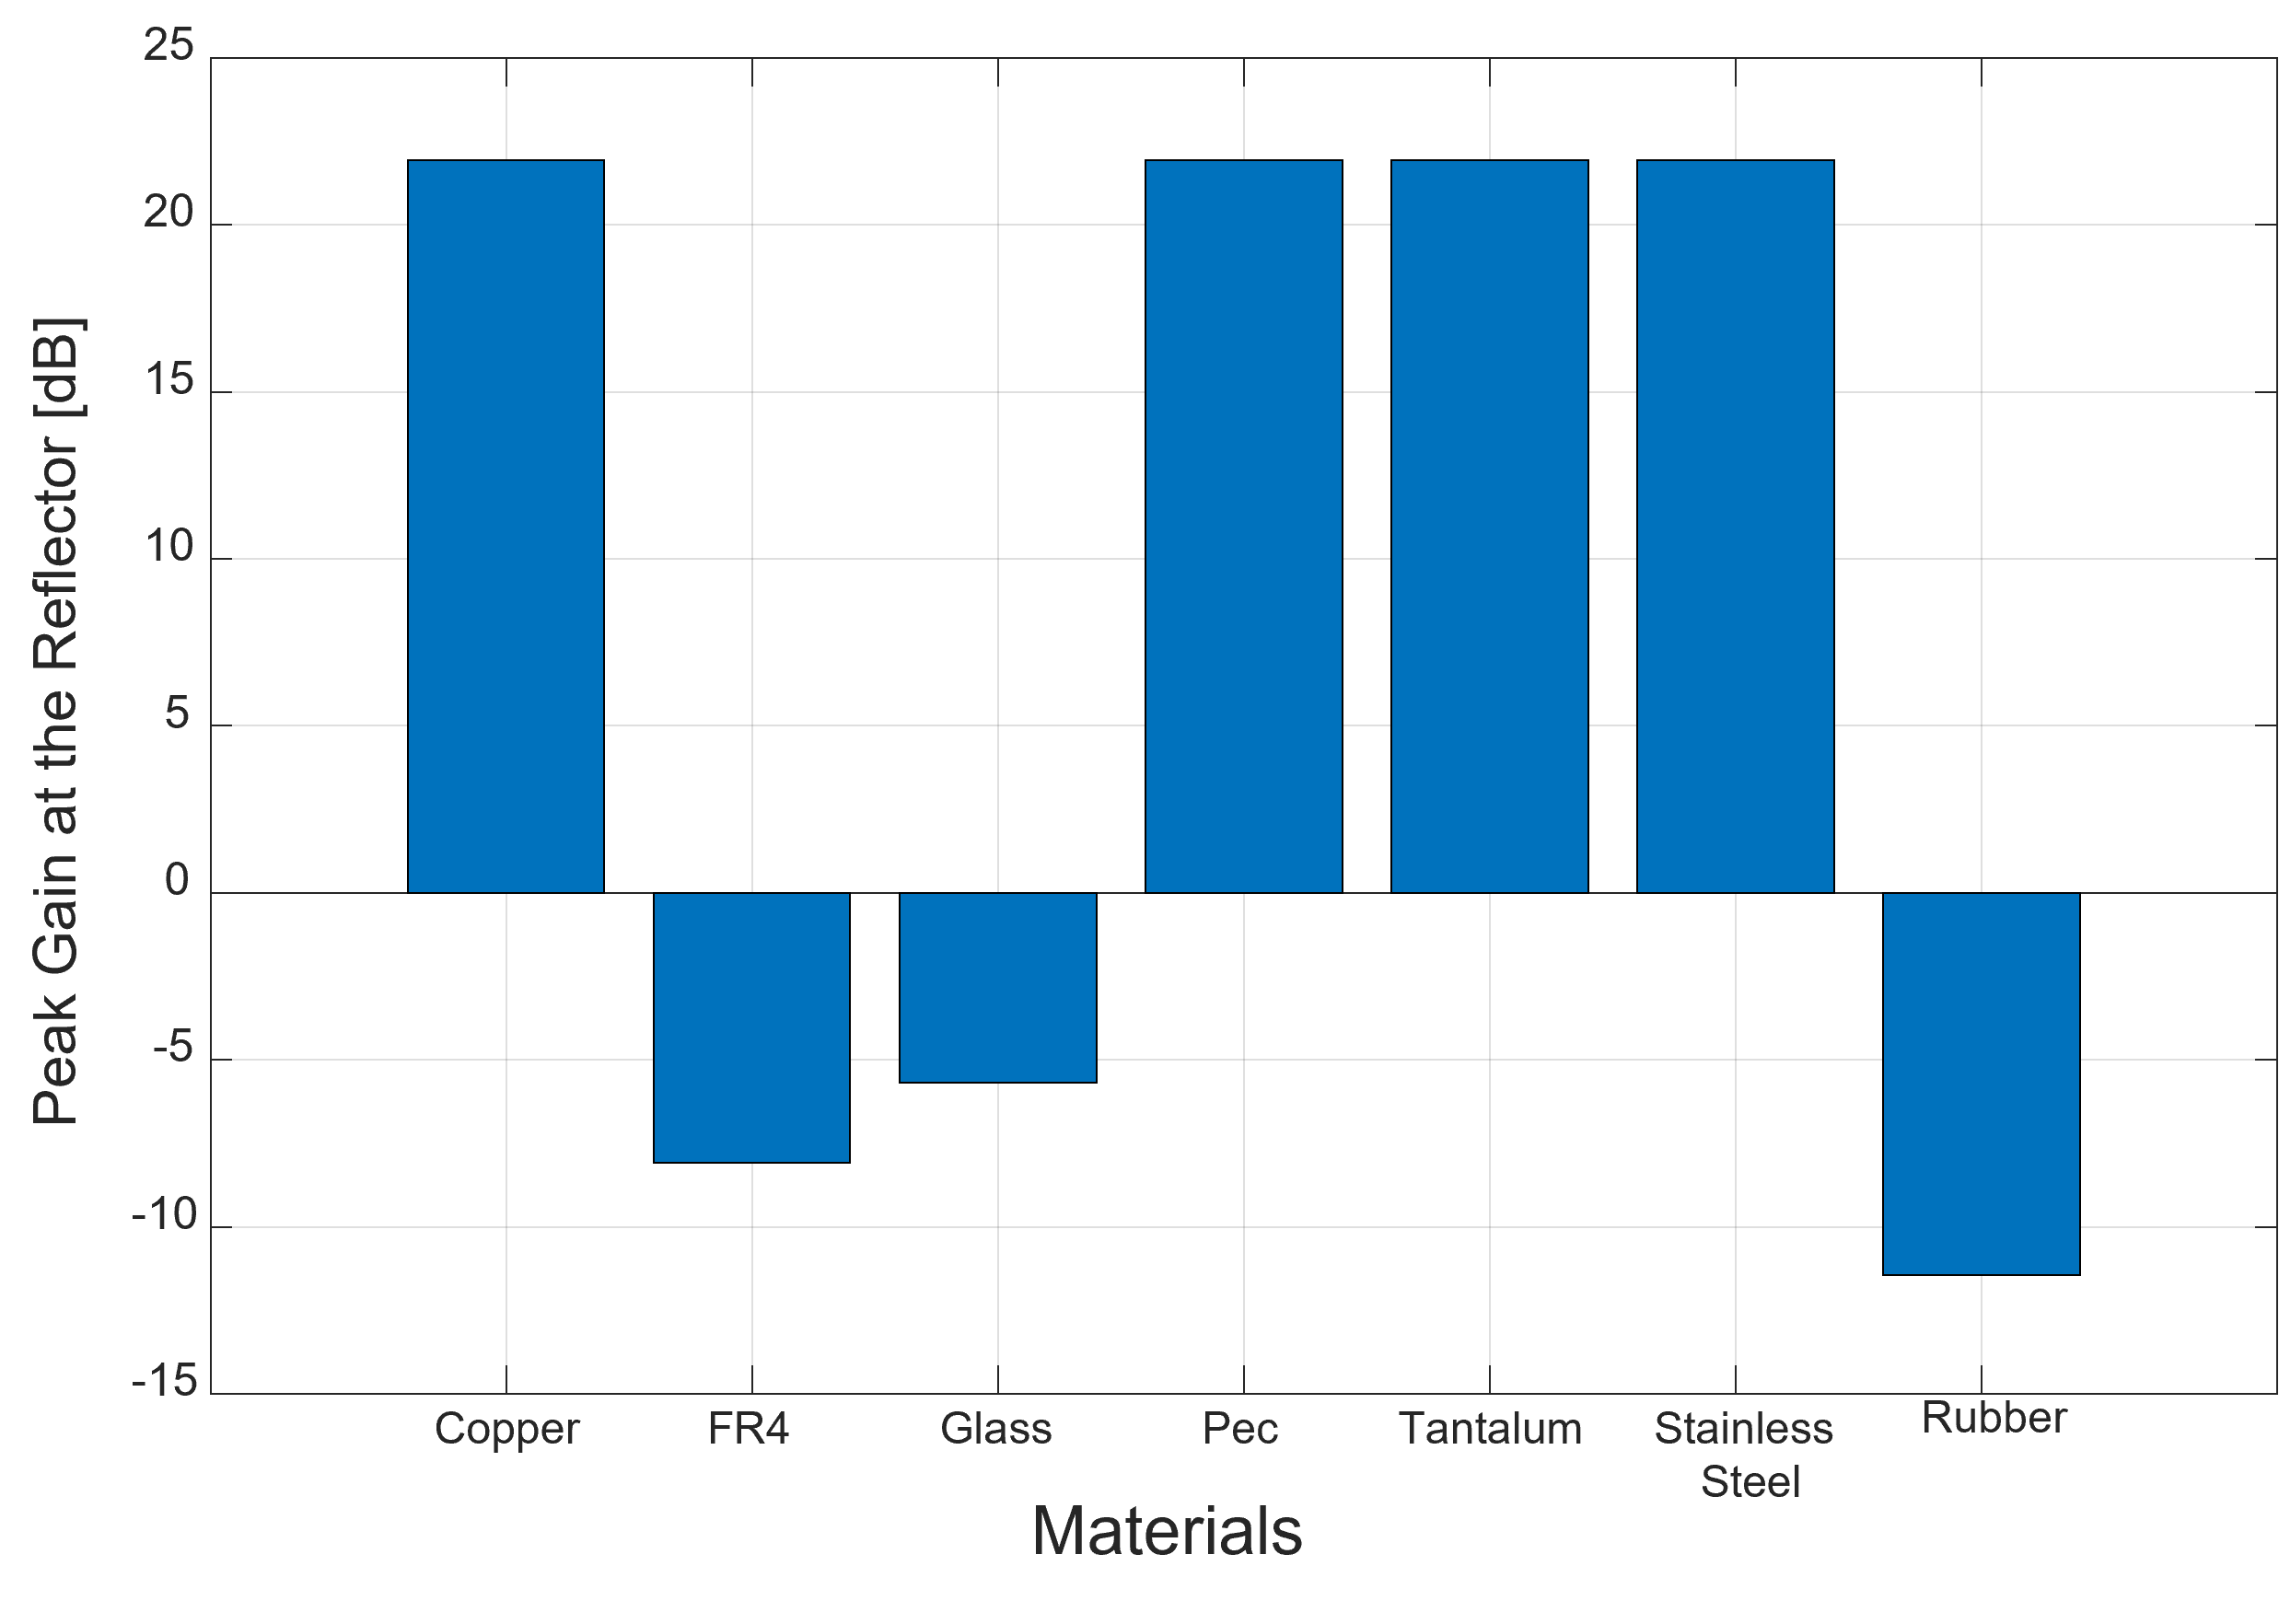
\includegraphics[width=0.5\linewidth]{images/Section 3 Images/Material1}
		\label{fig:conductivity1}
	}
	\hfill
	\subfloat[Peak reflection gains from simulations utilizing copper with modified conductivity as the base material of a HELIOS reflector module (blue). Linear regression curve (red) underlines roughly linear dependence on conductivity in the considered range.]{
		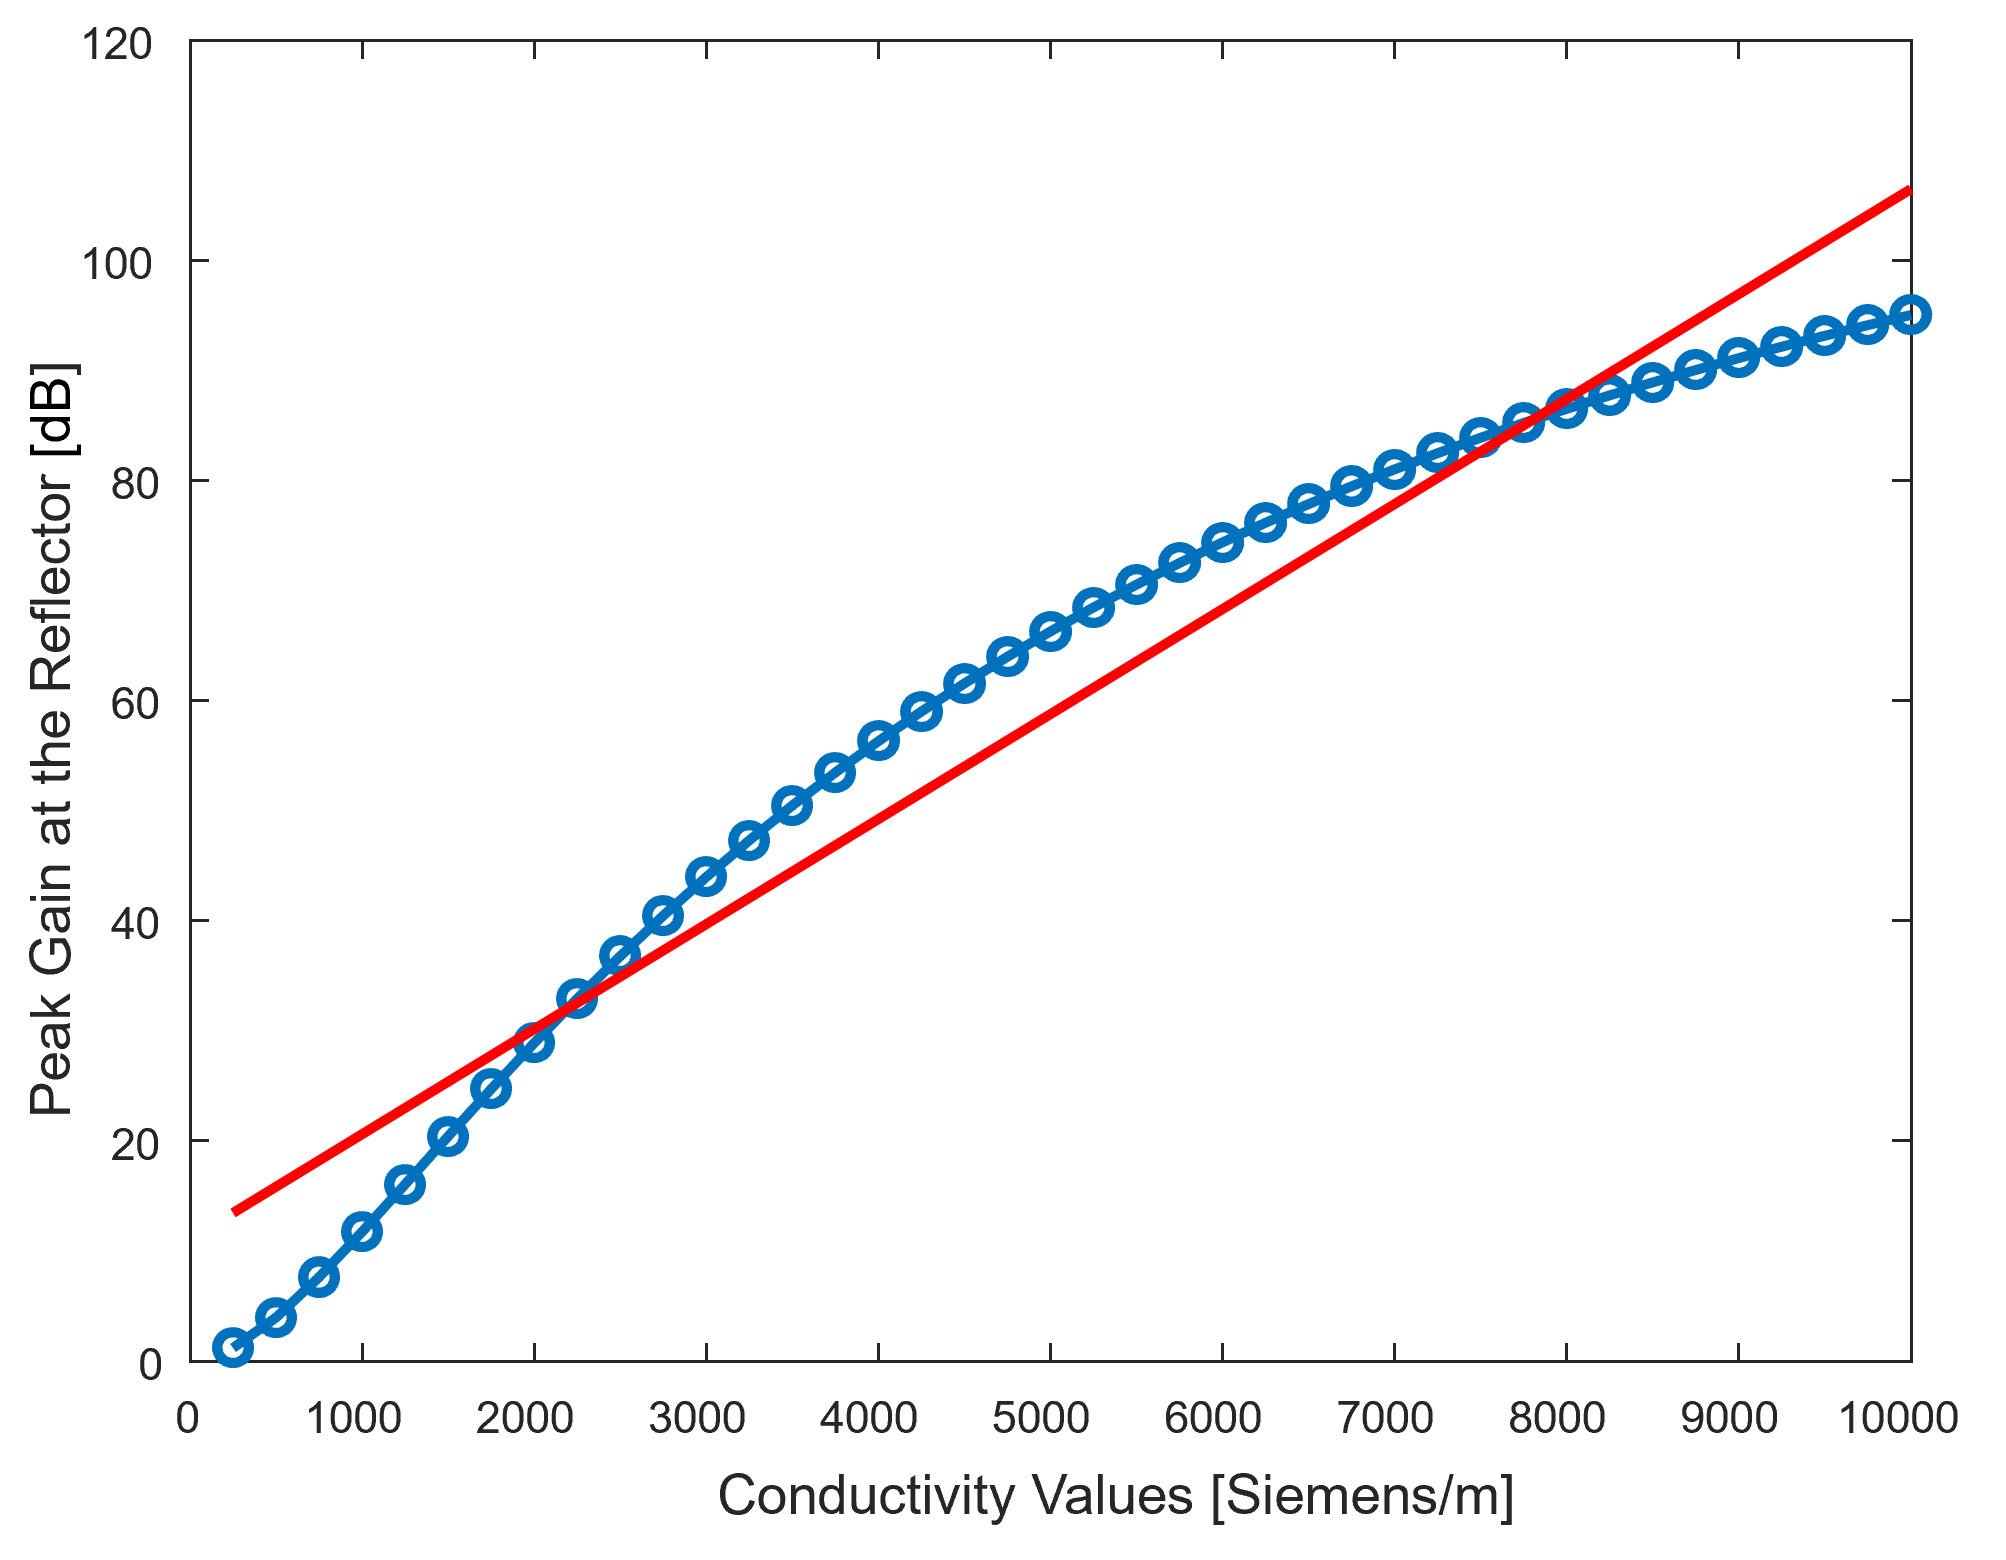
\includegraphics[width=0.45\linewidth]{images/Section 3 Images/conductivity2}
		\label{fig:conductivity2}
	}
	\caption[The influence of a reflecting surface on gain for various materials based on their conductivity and relative permittivity.]{The influence of a reflecting surface on gain for various materials based on their conductivity and relative permittivity.}
	\label{}
\end{figure}
\section{Analytical Modeling of HELIOS Modules} \label{Analytical Modeling of HELIOS Modules}
This section makes the crucial first step in developing the analytical model for the reflection characteristics of HELIOS reflectors by first considering only an individual HELIOS module. This is in coordination with the simulation results in \Cref{Simulative Analyses of HELIOS Reflector Modules} and the analytical models for IRSs in \Cref{coordinate systems}. For this purpose, we introduce the notion of the radar cross section in \Cref{Radar-Cross-Section and Radar Equation} which was already previously set to be the solution type of the EM wave simulator, cf. \Cref{sec:Simulation Methodology}. In \Cref{Transfer and Adaption of Model to HELIOS Modules}, we will discuss how RCS can be analytically adapted to HELIOS reflectors by also doing assessments with the EM simulation results in \Cref{Assessment of Differences between Simulations and Analytical Model}.
\subsection{Bistatic Radar Cross Section} \label{Radar-Cross-Section and Radar Equation}
The \ac{RCS} concept is a crucial tool in this thesis. It allows us to characterize how objects, in this case, our HELIOS model, interact with electromagnetic waves. \ac{RCS} is a fundamental concept in radar engineering and electromagnetic scattering \cite{Balanis, Kerr1989PropagationOS}. When an object is illuminated by electromagnetic waves, usually carrying radar signals, the \ac{RCS} describes the scattered power per unit solid angle from the object. It offers information about how "visible" an object is to radar systems. By describing the RCS of HELIOS reflectors in this thesis, our model may be used to estimate how it will appear to wireless systems such as 5G/6G.

The radar equation below shows how the RCS $\sigma_{Meta}$ can be considered in a channel model \cite{RCS1}. But first, it needs to be determined as follows. The formula in \Cref{Eq:RCS_rtendsto inf} gives the common definition of the RCS, which is written as the limit of the distance $r$ to infinity.
\begin{equation} \label{Eq:RCS_rtendsto inf}
	\sigma_{Meta}= \lim_{r\to\infty} 4 \pi r^2 \frac{|E_{Rx}|^2}{|E_{Tx}|^2} ,
\end{equation}
where $\sigma_{Meta}$ \footnote{$\sigma_{Meta}$ has an additional unit of $\si{\meter}^2$ and for simplicity, we mention \si{\decibel} instead of \si{\decibel}sm.} \footnote{The term "Gain" refers to the RCS, as elucidated in \Cref{Analytical Modeling of HELIOS Modules}, throughout this work.} is the RCS for the metasurface, and $E_{Rx}$ and $E_{Tx}$ are the far-field reflected and incident electric field intensities, respectively. As such, it is the ratio of incident and reflected wave in the infinite far-field. Fixing the direction of the incident wave and varying the considered reflection angle, the RCS becomes a multivariate reflection pattern similar to an antenna pattern \cite{RCS_1, RCS_2}. \Cref{Table:standard_sigma_values} below provides the standard RCS values that are usually encountered in the communication link. A non-zero $\sigma_{Meta}$ becomes relevant to account for real-world situations, including the existence of obstructions like a car within the communication channel. On the other side of the coin, a car typically comes with an RCS of \SI{20}{\decibel}sm, which is larger than the \SI{0}{\decibel}sm of a person, according to \Cref{Table:standard_sigma_values}.

\begin{table}[tb] % H -> dieses objekt wird genau da wo der code steht festgenagelt
	\caption{Standard RCS values which are commonly observed \cite{RCS_meta, RCS_meta2}.}
	\footnotesize
	\label{Table:standard_sigma_values}
	\centering
	\begin{tabular}{c|c}
		\textbf{Object} & \textbf{$\sigma_{Meta}$ [dBm]} \\
		\hline
		Man & \num{0}\\
		\hline
		Small bird & \num{-20}\\
		\hline
		Car & \num{20}\\
		\hline
		Large commercial airplane  & \num{20}\\
		\hline
		Small fighter plane  & \num{3}\\
	\end{tabular}
\end{table}
The application of bistatic RCS analysis necessitates a thorough comprehension of important variables, especially the angles of the incidence and departure which are crucial for evaluating randomly shaped scattering objects, in literature also referred to as radar targets \cite{Balanis, RCS2}.

The main reflection angle and magnitude of the scattered signal are strongly dependent on the angle of the incident and the shape of the object. To fully understand bistatic RCS one must first study the monostatic RCS, which is concerned with calculating the power reflected to the transmitting node \cite{RCS_3}. When the transmitter and receiver are in the same place, monostatic RCS measures the amount of power that a scatterer reflects to the transmitting node, hence indicating the visibility of an object. Conversely, bistatic RCS measures reflected power when the transmitter and receiver are at different sites. This latter case is thus more relevant for 5G/6G mmWave communications, although the monostatic RCS can be of interest for future 6G \ac{JCAS} use cases.
\subsection{Analytical Model for the Reflection of Planar Surfaces} \label{Analytical Model for the Reflection of Planar Surfaces}
In literature, one may find a formula for the bistatic RCS of a rectangular plate. It depends on the following parameters:
\begin{itemize}
	\item Plate dimensions and materials
	\item Carrier frequency
	\item Angles of incident and reflected wave
\end{itemize}
Taking into account the above-mentioned parameters, RCS formulas have been derived in literature \cite{Helios, Kerr1989PropagationOS, Balanis} as follows:
\begin{equation} \label{RCS_flatplate}
	\begin{aligned}
	\sigma_{plate} = 4 \cdot \pi \cdot \left( \frac{a \cdot b}{\lambda} \right)^2 \cdot \cos^2 \left( \theta_{Rx} \right) \cdot \sinc^2 \left( \frac{\pi \cdot b \cdot \left( \sin \left(\theta_{Rx} \right) \cdot \sin \left( \varphi_{Rx} \right) \pm \sin \left( \theta_{Tx} \right) \right) }{\lambda} \right) \\
			\begin{cases}
		+, & \varphi_{Rx}= \frac{3\cdot \pi}{2} \\
		-,  & \varphi_{Rx}= \frac{\pi}{2}
	\end{cases} 
	\end{aligned}
\end{equation}
\Cref{RCS_flatplate} gives the \ac{RCS} equation for a flat plate reflecting surface with dimensions $a$ and $b$ that operate at wavelength $\lambda$. This equation includes three critical supported angles: the incident elevation angle $\theta_{Tx}$, the reflected elevation angle $\theta_{Rx}$, and the azimuth angle of the receiving radar system $\varphi_{Rx}$. Notably, in the context of the reference used in our study \cite{Balanis}, a specific assumption is made about the value of the incident azimuth angle $\varphi_{Tx}$, which is retained constant to $0^\circ$. In \Cref{RCS_flatplate}, the flatplate's orientation concerning the radar system is indicated by the different $\pm$ symbols for $\sin(\theta_{Rx})$, $\sin(\varphi_{Rx})$, and $\sin(\theta_{Tx})$. In particular, the minus symbol indicates the flatplate's front side, indicating that the side facing the radar transmitter and receiver is where incident radar waves interact. Whereas, the side opposite the incident radar waves is represented by the plus symbol, where the radar waves interact with the flatplate's hidden or obscured side. We concentrate on the front side of the plate for this thesis since it is oriented in a way that directly interacts with the radar system and offers important information about the RCS properties of the flatplate in our analytical framework.
\subsection{Modeling of HELIOS Module Reflection} \label{Transfer and Adaption of Model to HELIOS Modules}
Having provided the fundamental \ac{RCS} equation for a flat plate reflector in \Cref{RCS_flatplate}, we now need to modify the equation for use in the context of wireless communications and to match it to the HELIOS concept, as illustrated by \Cref{Eq:RCS_flatplate_dependency}, and \Cref{Eq:RCS_HELIOS_dependency}. In this section, we will delve into the complexities of these modifications, illuminating the changes and adjustments made to attain the appropriate alignment.
\begin{equation}\label{Eq:RCS_flatplate_dependency}
	\sigma_{Plate}(a, b, \lambda, \theta_{Tx}, \theta_{Rx}, \varphi_{Rx})
\end{equation}
\begin{equation}\label{Eq:RCS_HELIOS_dependency}
	\sigma_{Module}(a, b, \alpha, \beta, \lambda, \theta_{Tx}, \varphi_{Tx}, \theta_{Rx}, \varphi_{Rx})
\end{equation}
While the basic equation for a flat rectangular plate reflector provides a solid foundation, the unique characteristics of the HELIOS model need the inclusion of further parameter dependencies, i.e., $\varphi_{Tx}, \alpha$, and $\beta$, cf. \Cref{Eq:RCS_HELIOS_dependency}. 

\Cref{Table:Comparison flat plate and HELIOS} emphasizes the important changes made to develop the improved HELIOS equation. The dimensions of a flat plate are $a \times b$, which is basically with slope angles $\alpha=\beta=0^\circ$, HELIOS introduces a more complex geometry with dimensions that vary dynamically with $a, b, \alpha$, and $\beta$ values, as can be seen in \Cref{fig:HELIOS_footprint}. Another notable modification is the addition of the supported angle $\varphi_{Tx}$. Unlike the flat plate, we do not assume that $\varphi_{Tx}=0^\circ$.
\begin{table}[H] % H -> dieses objekt wird genau da wo der code steht festgenagelt
	\caption{Comparing the existing equation for flat plate, cf. \Cref{Eq:RCS_flatplate_dependency} which is used for the adaptation of our RCS equation for the HELIOS analytical module, cf. \Cref{Eq:RCS_HELIOS_dependency}, focusing on the changes implemented. }
	\footnotesize
	\label{Table:Comparison flat plate and HELIOS}
	\centering
	\begin{tabular}{>{\centering\arraybackslash}m{4cm}|>{\centering\arraybackslash}m{4cm}|>{\centering\arraybackslash}m{6cm}}
		Aspects & \begin{tabular}{@{}c@{}} Equation for flat plate,\\cf. \Cref{Eq:RCS_flatplate_dependency} 	\end{tabular}&  \begin{tabular}{@{}c@{}} Equation for the HELIOS module,\\cf. \Cref{Eq:RCS_HELIOS_dependency}	\end{tabular}\\
		\hline
		\begin{tabular}{@{}c@{}}Reflecting surface \\ size \end{tabular} & $a \cdot b$ &  $a \cdot \sqrt{1+\tan^2(\alpha)} \cdot b \cdot \sqrt{1+\tan^2(\beta)}$ \\[2ex]
		\hline
		Supported angles & $\theta_{Tx}, \theta_{Rx}, \varphi_{Rx}$ &  $\theta_{Tx}, \theta_{Rx}, \varphi_{Tx}, \varphi_{Rx}$\\[2ex]
		\hline
		Rotation of reflecting surface & none, fixed to $y$-$z$-plane & \begin{tabular}{@{}c@{}c@{}c@{}c@{}}Substitute angles by: \\ 
			$\theta_{Tx} \gets (\theta_{Tx} - \beta)$\\
			$\theta_{Rx} \gets (\theta_{Rx} - \beta)$\\
			$\varphi_{Tx} \gets (\varphi_{Tx} - \alpha)$\\
			$\varphi_{Rx} \gets (\varphi_{Rx} - \alpha)$\\
		\end{tabular}\\
		\hline
		Beamwidth correction factor in $\sinc$ argument & 1  &  $\frac{1}{2}$
	\end{tabular}
\end{table}
In the above figure, HELIOS footprint with size $a\times b$ is the flatplate dimensions, whereas the HELIOS reflecting surface's dimension is ($a \cdot \sqrt{1+\tan^2(\alpha)} \times b \cdot \sqrt{1+\tan^2(\beta)}$ ).

\begin{figure}[tb]
	\centering
	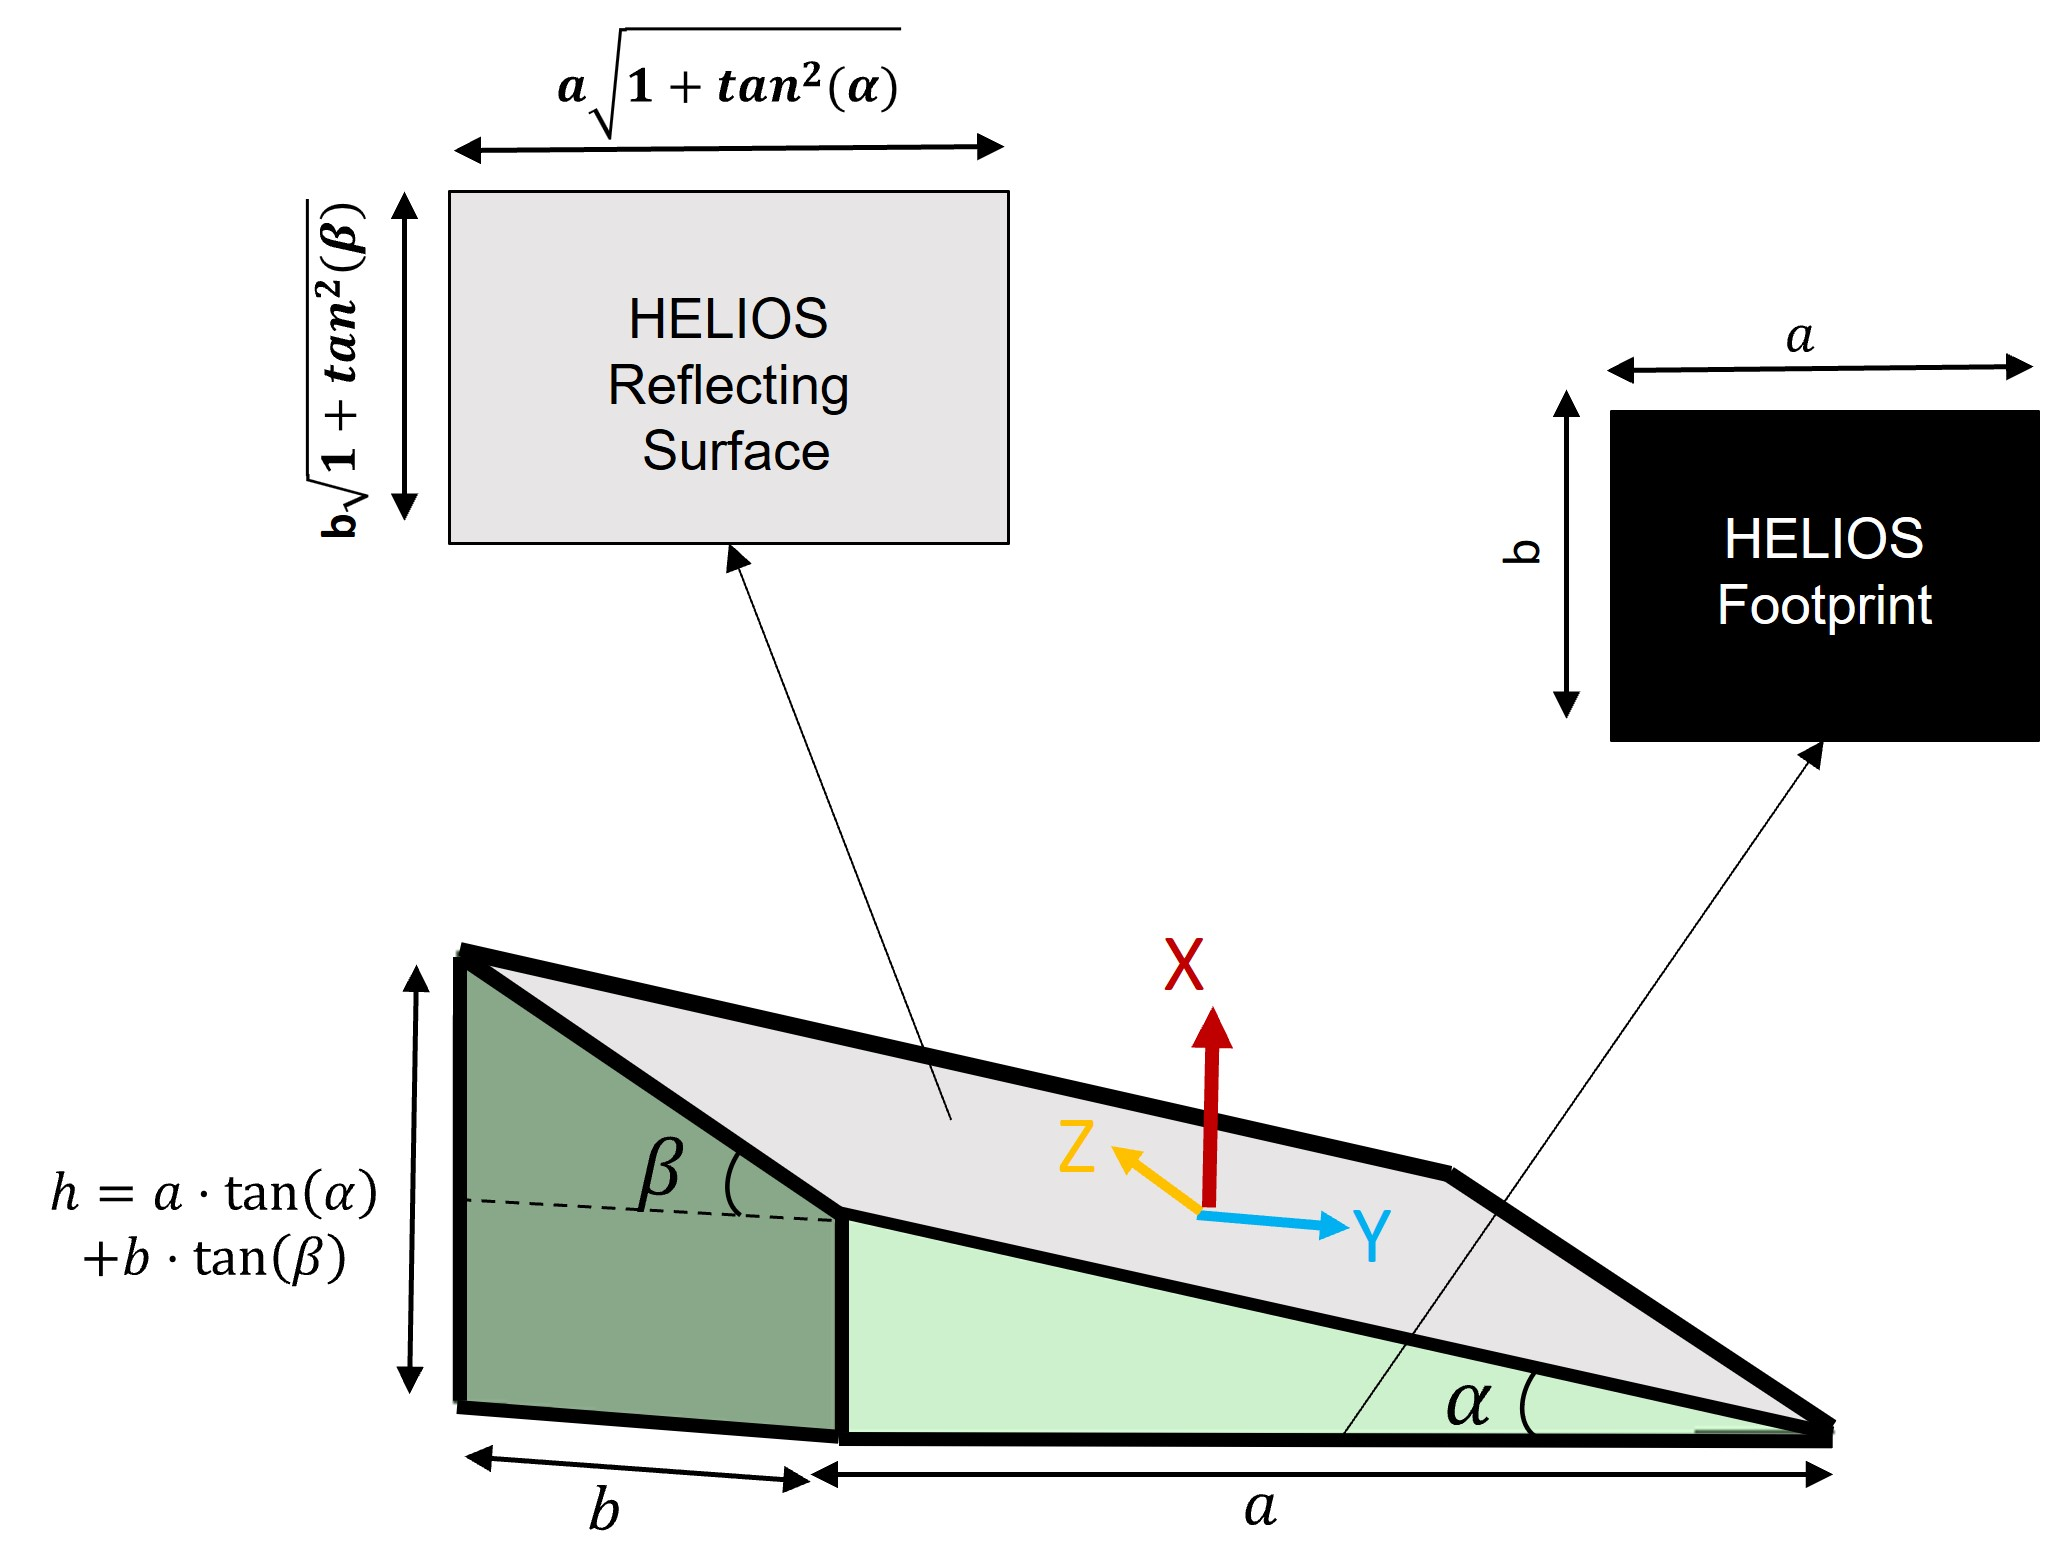
\includegraphics[width=0.5\linewidth]{images/Section 3 Images/HELIOS_footprint}
	\caption{Geometric relation between HELIOS footprint size given by ($a \cdot b$), and reflecting surface size given by ($a \cdot \sqrt{1+\tan^2(\alpha)} \cdot b \cdot \sqrt{1+\tan^2(\beta)}$), where $a$ and $b$ are the length and width of the module.}
	\label{fig:HELIOS_footprint}
\end{figure}
Furthermore, the slope angles $\alpha$, and $\beta$ of the HELIOS module affect the main lobe reflection angles $\theta_{Rx}$ and $\varphi_{Rx}$ as summarized by \Cref{HELIOS 2times beta} and \Cref{HELIOS 2times alpha}. As the Snell's law still holds along the shifted surface's normal vector, this rotation aspects is implemented by a coordinate transformation shifting by $\alpha$, and $\beta$. As a result, the angles of incidence $\theta_{Tx}$ and $\varphi_{Tx}$ in the equation are replaced by $\theta_{Tx}-\beta$ and $\varphi_{Tx}-\alpha$. The same holds for the angles of departure. To ensure that the beamwidth matches the simulated values, the literature already includes a scaling factor $\frac{1}{2}$ by default, allowing for a more precise match of the theoretical model with a HELIOS module's real-world behavior.

Based on all of the above changes, an individual HELIOS module exhibits the following bistatic RCS holding for $\theta_{Tx}$, $\varphi_{Tx}$, $\theta_{Rx}$, and $\varphi_{Rx} \in [-90, 90]^\circ$:

$	\sigma_{module}= 4 \cdot \pi \cdot \Gamma \cdot \left( \frac{\left( a \cdot \sqrt{1+\tan^2(\alpha)}\right) \cdot \left( b \cdot \sqrt{1+\tan^2(\beta)} \right) }{\lambda} \right) ^2 \left( \cos^2 \left( \theta_{Tx}-\beta \right) \cdot \cos^2 \left( \theta_{Rx}-\beta \right) \cdot \cos^2 \left( \varphi_{Rx}-\alpha \right) \right)$
\begin{equation} \label{Eq:HELIOS_module}
	\begin{aligned}
		& \left( \sinc \left( \frac{1}{2} \cdot k \cdot b \cdot \sqrt{1+\tan^2(\beta)} \cdot \left( \sin \left( \theta_{Rx}-\beta \right) \cdot \cos \left( \varphi_{Rx}-\alpha \right) -\sin \left( \theta_{Tx}-\beta \right) \cdot \cos \left( \varphi_{Tx}-\alpha \right) \right) \right) \right)^2\\
		&  \left( \sinc \left( \frac{1}{2} \cdot k \cdot a \cdot \sqrt{1+\tan^2(\alpha)} \cdot \left( \cos \left( \theta_{Rx}-\beta \right) \cdot \sin \left( \varphi_{Rx}-\alpha \right) -\cos \left( \theta_{Tx}-\beta \right) \cdot \sin \left( \varphi_{Tx}-\alpha \right) \right) \right) \right)^2 
	\end{aligned}
\end{equation}
Two $\sinc$ functions are presented in the equation, each of which individually affects the surface size's reflection properties for length and width. For the target's radar cross-section to be adequately represented, this separation is necessary. The diffraction phenomenon's $\sinc$ functions explain the reflecting surface's spatial extent along its dimensions, providing a thorough representation of the target's scattering characteristics. The equation provides a more accurate and complete model for radar analysis by accounting for the distinct impacts of width and length on the reflected signal.

The insertion of the adjustments mentioned in the \Cref{Table:Comparison flat plate and HELIOS} into the fundamental \Cref{RCS_flatplate} for a flat plate reflector leads to \Cref{Eq:HELIOS_module}, constituting our analytical model for the bistatic RCS of an individual HELIOS module.
\subsection{Assessment of Differences between Simulations and Analytical Model} \label{Assessment of Differences between Simulations and Analytical Model}
In this section, we will conduct a detailed comparison of EM simulations and our previously provided analytical model to check matching properties and, in particular, to determine the extent to which there are discrepancies.

\Cref{fig:absweep} shows the link between peak gain, defined as $\max\left(\sigma_{Module}\left(\varphi_{Rx}, \theta_{Rx}\right)\right)$, attained and reflector width $b$ in \si{\centi\meter}. The upper curves show the quadratic case in which $a=b$ in the range from \num{1} to \SI{100}{\centi\meter}, whereas the lower curves show the rectangular case in which $a$ is fixed to \SI{10}{\centi\meter} and $b$ again varies between \num{1} to \SI{100}{\centi\meter}. These curves are based on our study in \Cref{Simulative Analyses of HELIOS Reflector Modules} and related work in \Cref{coordinate systems}, show a steady increase in gain as the reflector size increases. Notably, one observes a strong match between simulations and our analytical model. Both the curves from the analytical model and EM simulation results meet when $a=b=\SI{10}{\centi\meter}$.
\begin{figure}[H]
	\centering
	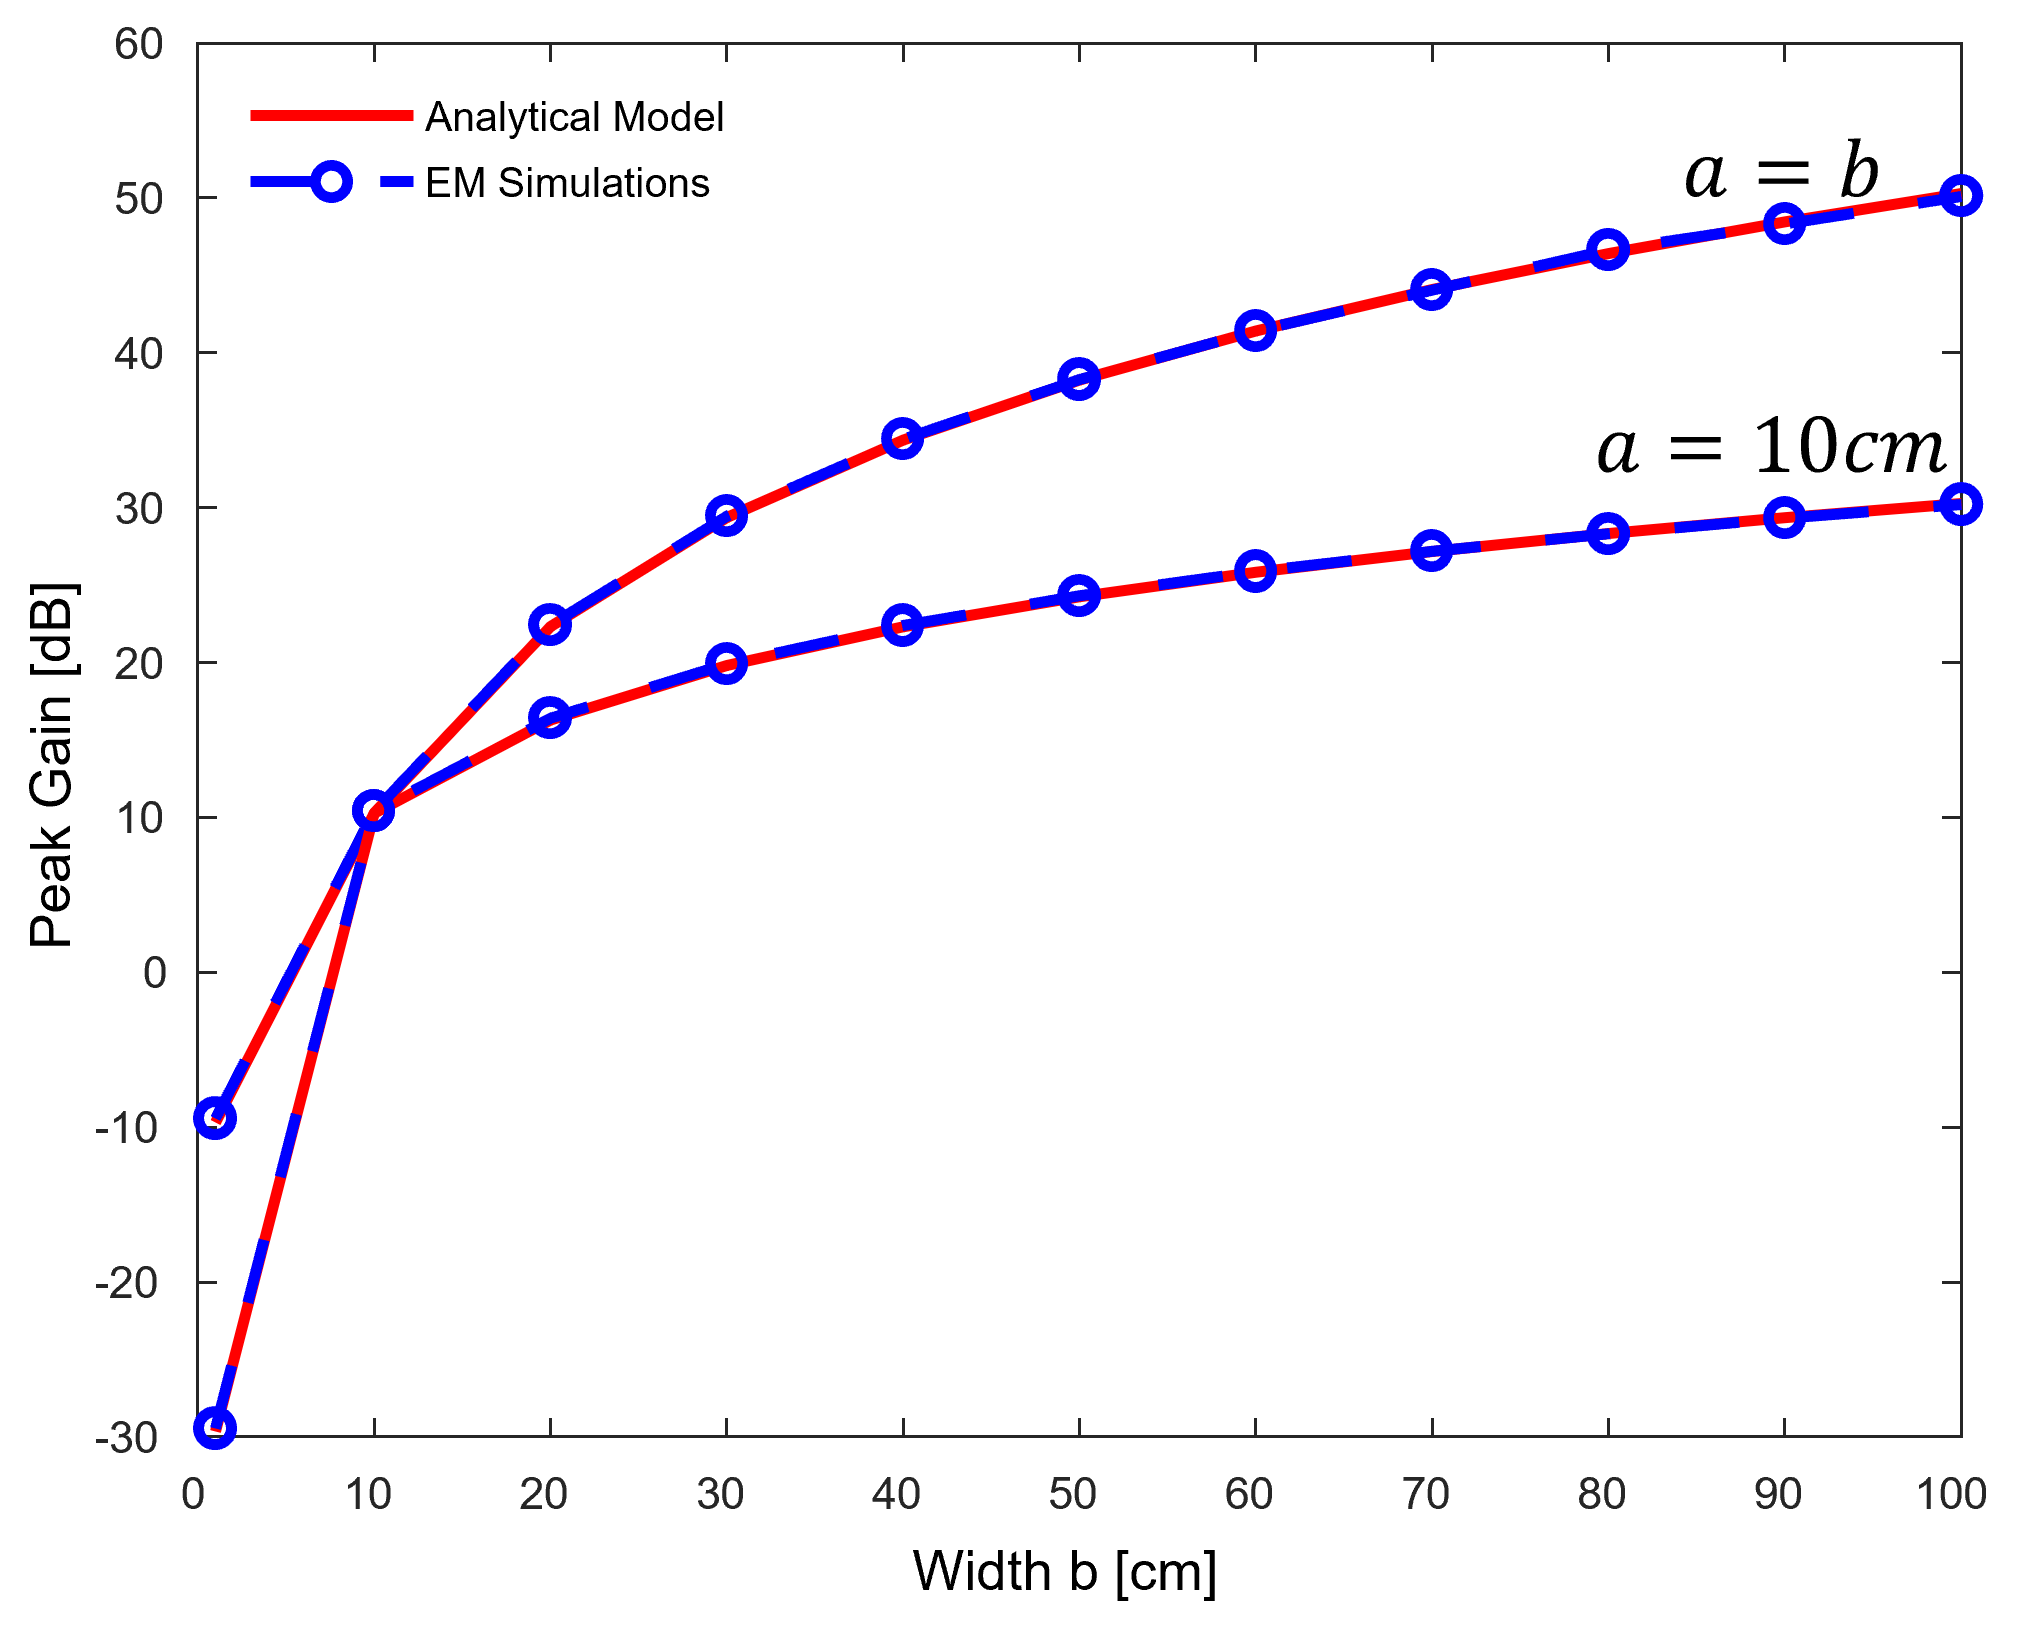
\includegraphics[width=0.7\linewidth]{images/Section 3 Images/a_b_sweep}
	\caption{Comparison of peak RCS value yielded by simulation and analytical model for rectangular $(\SI{10}{\centi\meter} \times b)$ and quadratic $(b \times b)$ HELIOS module footprints, where we observe a matching behavior. Further parameters: $\varphi_{Tx}=\theta_{Tx} = 0^\circ$ and, $\alpha_{m,n}=\beta_{m,n}=10^\circ$.}
	\label{fig:absweep}
\end{figure}

\Cref{fig:comparison1d} depicts the horizontal (left) and vertical (right) slices of the bistatic RCS patterns from both the simulations and analytical model, respectively, for HELIOS reflector modules configured with $a=\SI{10}{\centi\meter}$, $b=\SI{20}{\centi\meter}$, $\alpha=\num{10}^\circ$, and $\beta=\num{5}^\circ$, and given a \SI{28}{\giga\hertz} incident wave from direction $\varphi_{Tx}=\theta_{Tx}=\num{0}^\circ$.
\begin{figure}[tb]
	\centering
	\subfloat[Azimuth angle $\varphi_{Rx}$ variation for a HELIOS module when $\theta_{Rx}=0^\circ$ highlighting a match near the main lobe (green color) and a mismatch occurs further away (red color). ]{
		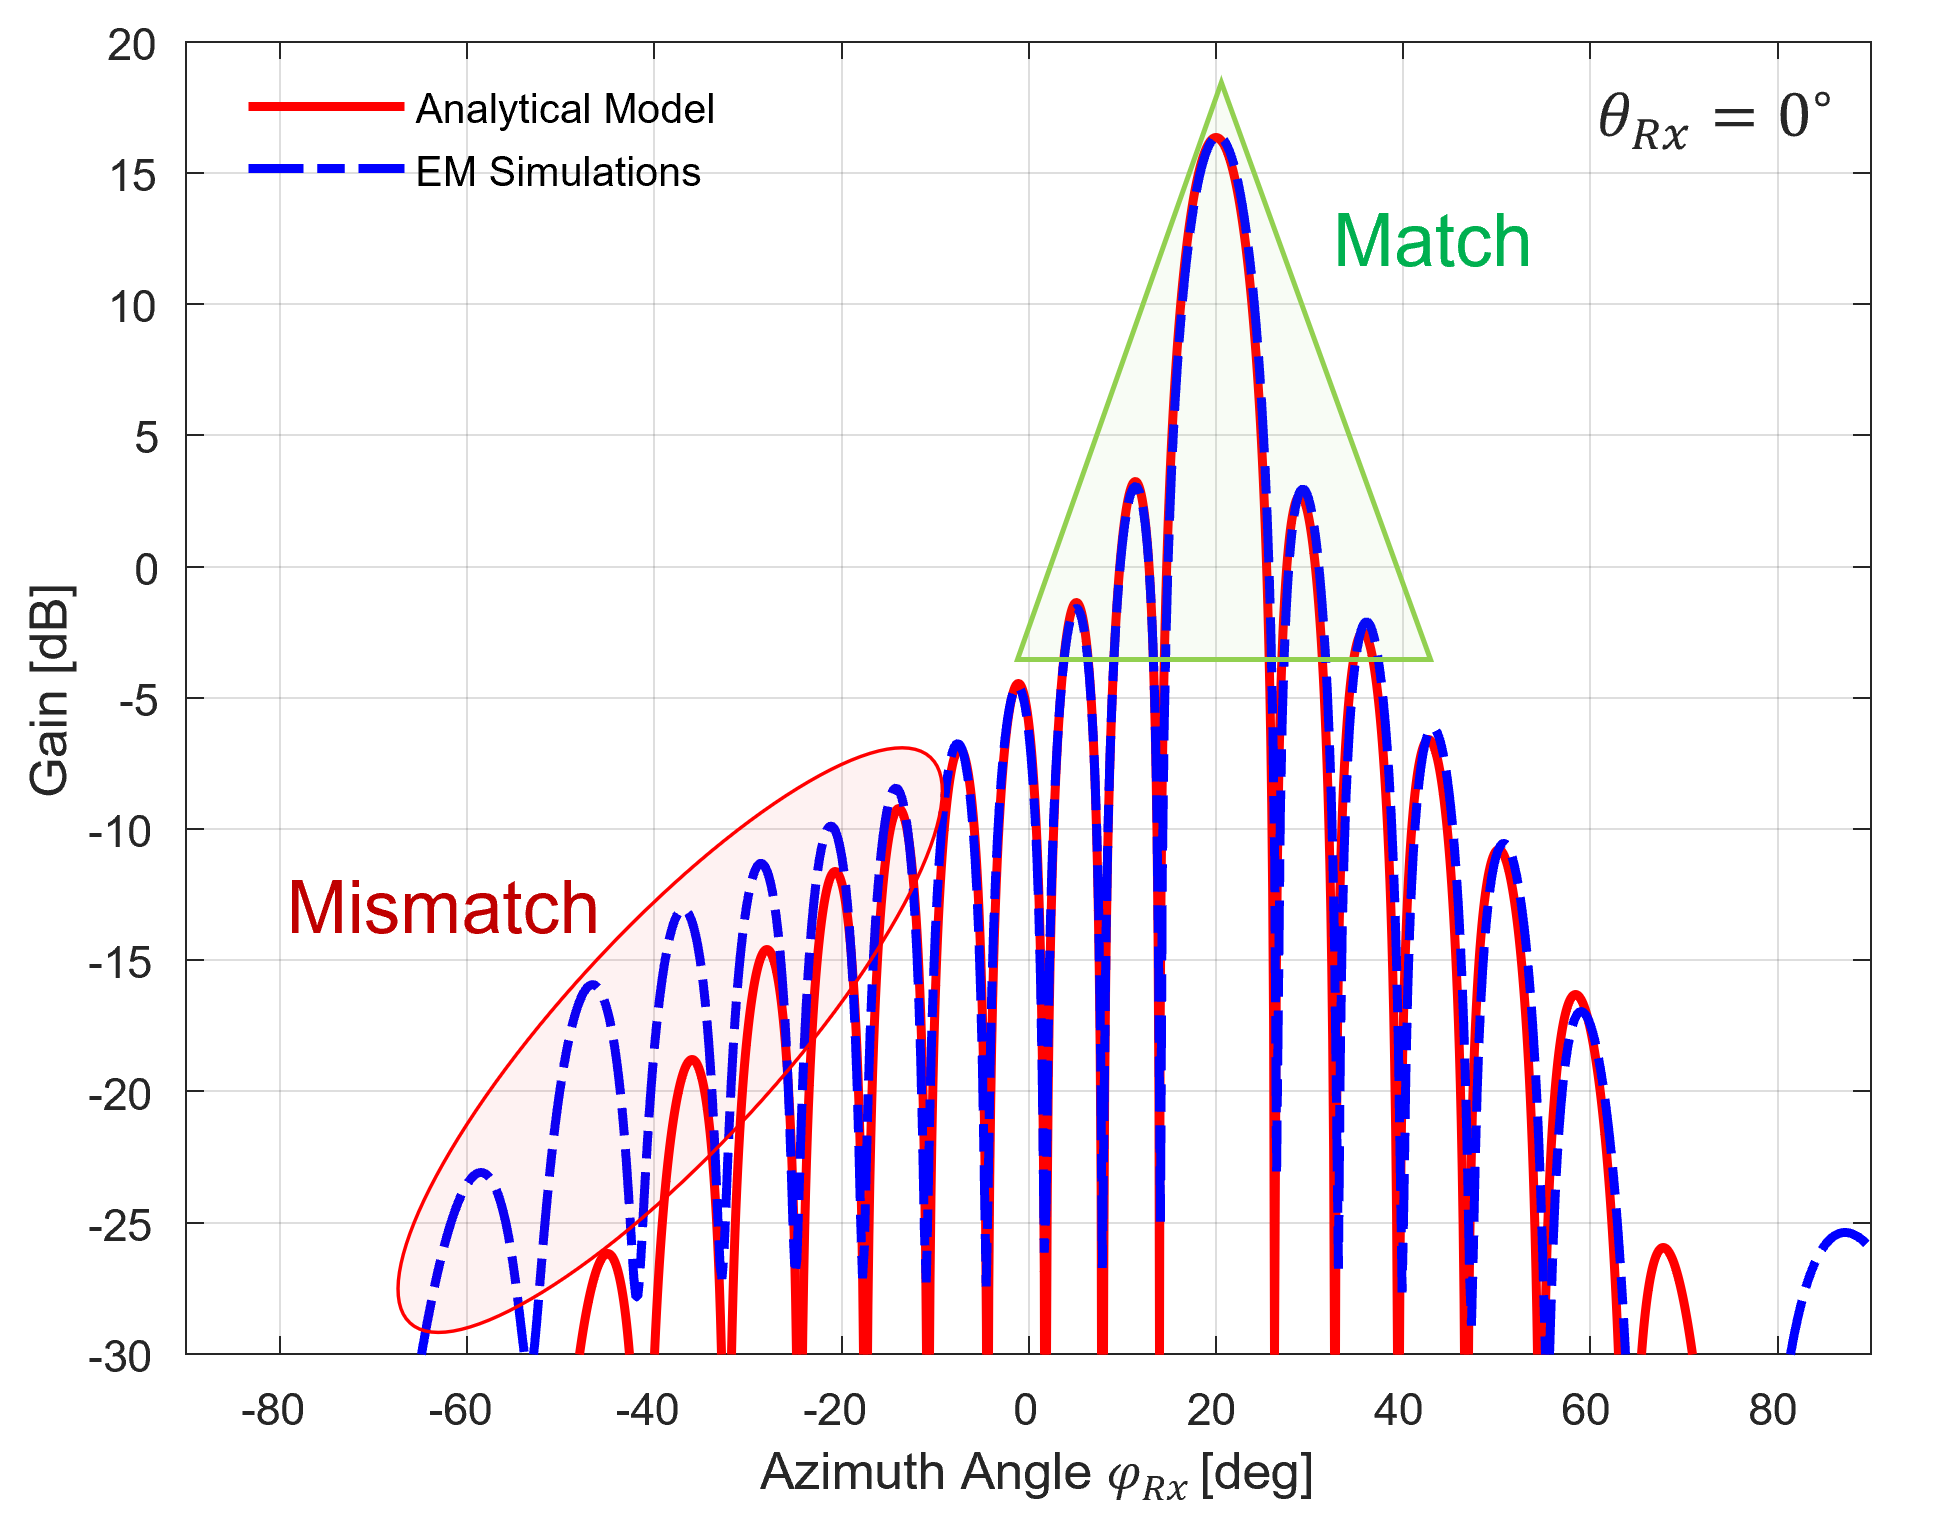
\includegraphics[width=0.46\linewidth]{images/Section 3 Images/comparison_1D_a}
		\label{fig:comparison1da}
	}
	\hfill
	\subfloat[Elevation angle $\theta_{Rx}$ variation for a HELIOS module when $\varphi_{Rx}=0^\circ$ highlighting a match (green color) overall.]{
		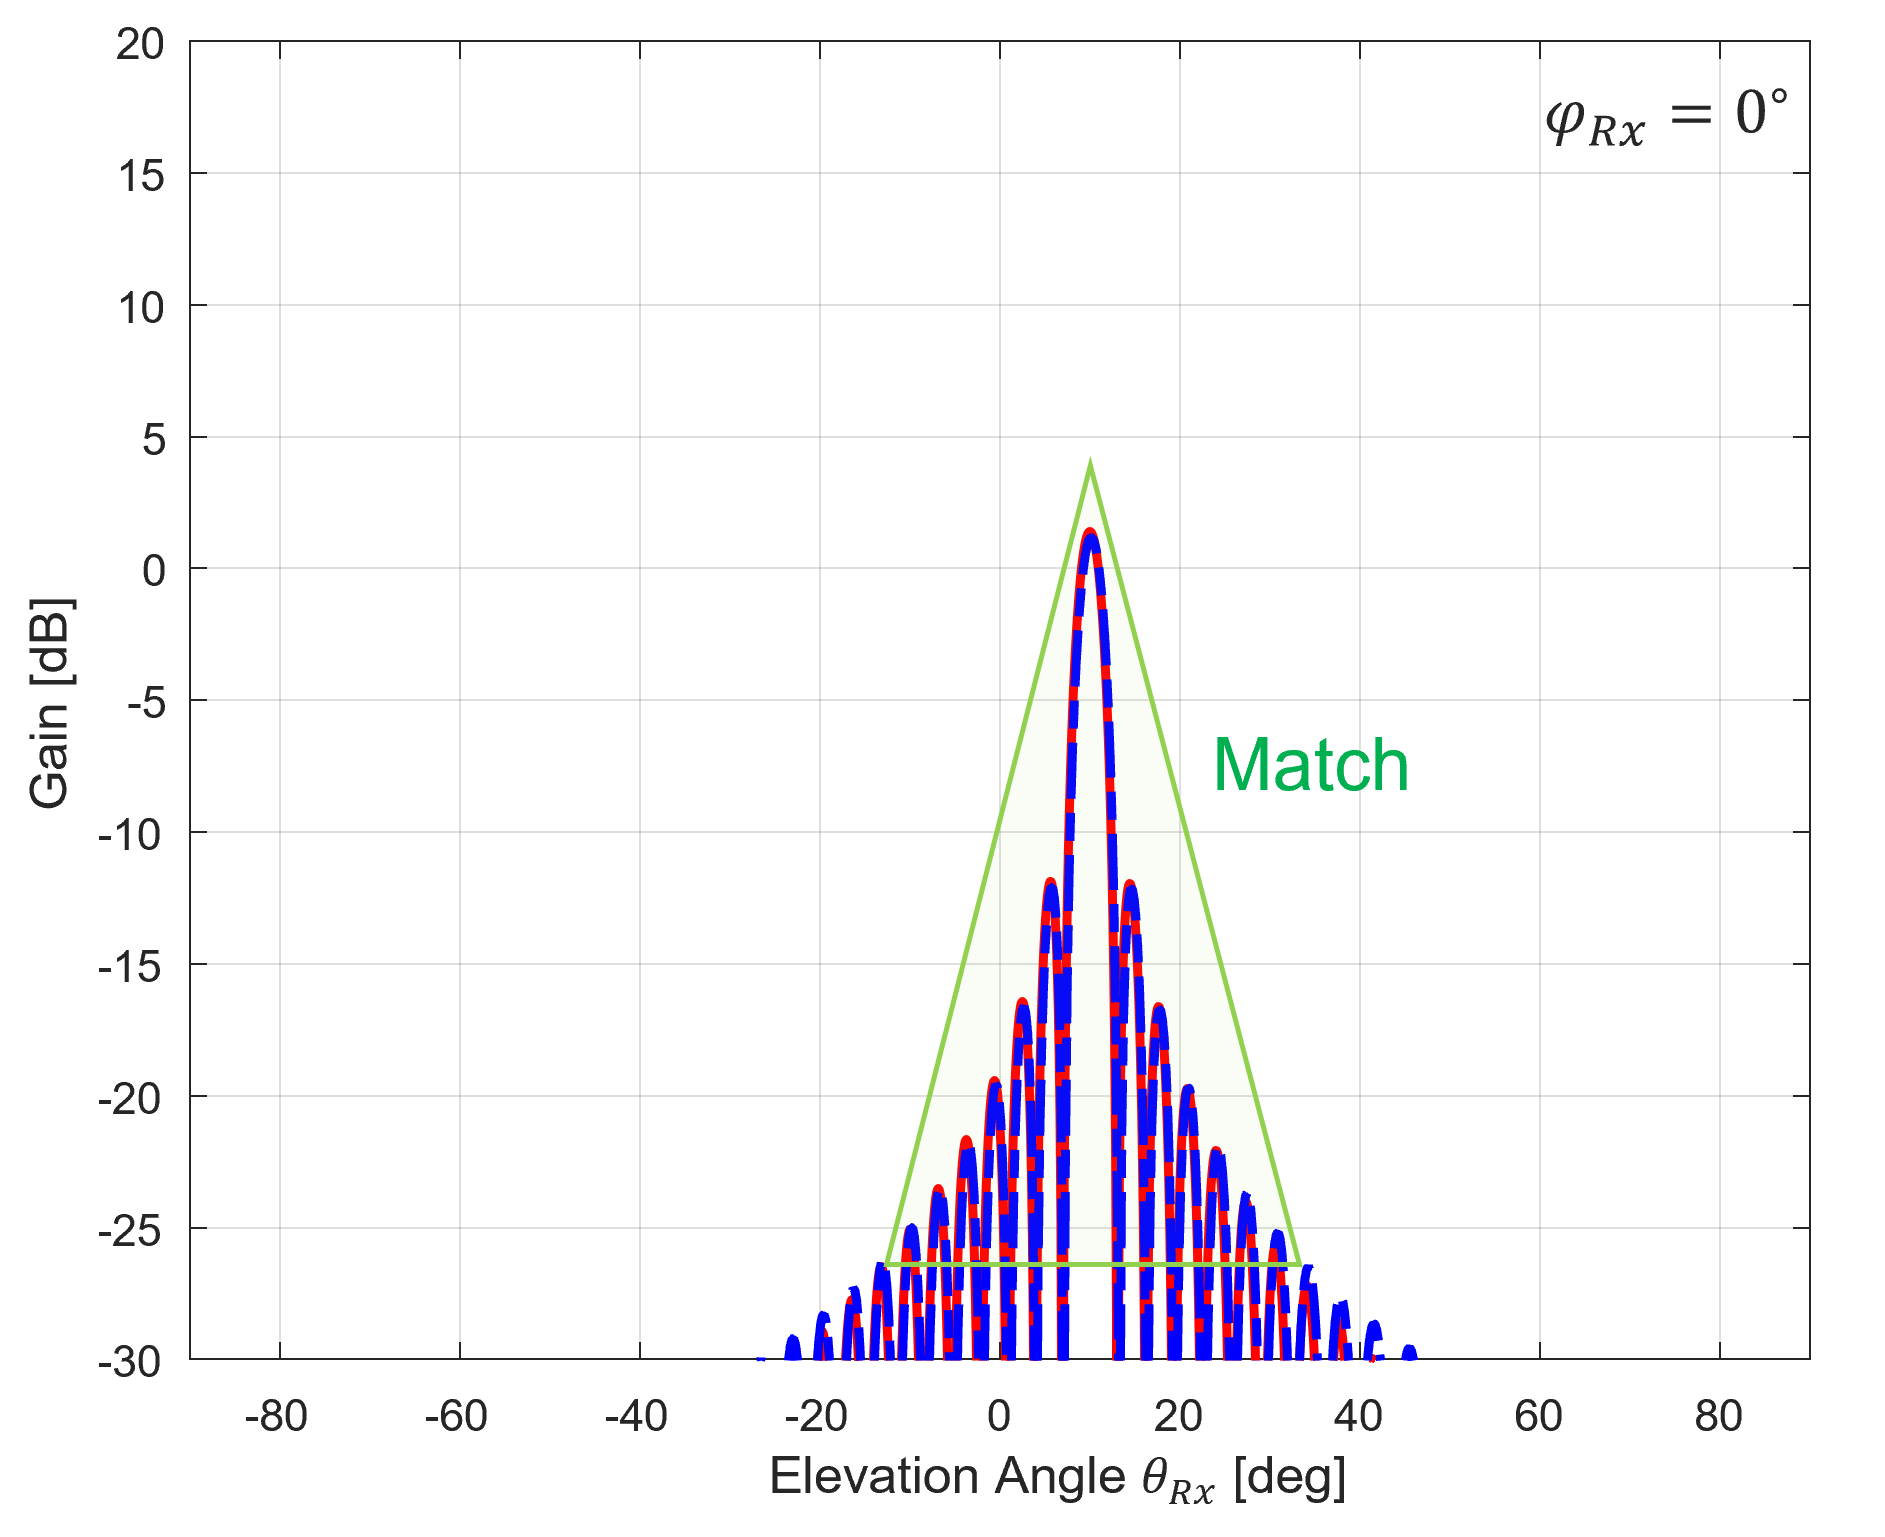
\includegraphics[width=0.45\linewidth]{images/Section 3 Images/comparison_1D_b}
		\label{fig:comparison1db}
	}
	\caption[Validating the HELIOS concept along azimuth and elevation angle at the receiver and highlighting the similarities and differences between simulated and analytical models for a HELIOS module when $a=\SI{10}{\centi\meter}$, $b=\SI{20}{\centi\meter}$, $\alpha=\num{10}^\circ$, and $\beta=\num{5}^\circ$, and both $\varphi_{Tx}=\theta_{Tx}=\num{0}^\circ$. A notable match in the peak gain is observed between the simulation results and the analytical model.]{Validating the HELIOS concept along azimuth and elevation angle at the receiver and highlighting the similarities and differences between simulated and analytical models for a HELIOS module when $a=\SI{10}{\centi\meter}$, $b=\SI{20}{\centi\meter}$, $\alpha=\num{10}^\circ$, and $\beta=\num{5}^\circ$, and both $\varphi_{Tx}=\theta_{Tx}=\num{0}^\circ$. A notable match in the peak gain is observed between the simulation results and the analytical model.}
	\label{fig:comparison1d}
\end{figure}
In the horizontal pattern slice on \Cref{fig:comparison1da}, we observe the RCS peaks at $\varphi_{Rx} = 20^\circ = -\varphi_{Tx} + 2\cdot\alpha$, thus confirming \Cref{HELIOS 2times alpha}. Similarly, the vertical RCS pattern slices in \Cref{fig:comparison1db} confirm that the RCS peaks of simulation and analytical model are indeed at $\theta_{Rx} = 10^\circ = -\theta_{Tx} + 2\cdot\beta$, cf. \Cref{HELIOS 2times beta}. The beamwidth along $\varphi_{Rx}$ depends on reflector dimension $a$, whereas $\theta_{Rx}$ depends on $b$. In \Cref{fig:comparison1d}, as the dimensions $b >a$, the vertical beamwidth (right) is narrower than the horizontal (left).

The interesting part in both these figures is that the simulated values closely match the analytical values, displaying exceptional behavior in the properties of their main and the first-order, $N$-th-order side lobes. But farther from the main lobes we see the mismatch along the azimuth angle, as depicted in \Cref{fig:comparison1da} (red-colored). Our main region of interest shows a lot of similarities to that of simulated results (green-colored). Furthermore, a closer examination of these figures reveals the importance of beamwidth in the behavior of these systems which depends on the size of the reflector.

\Cref{fig:heatmap1d} shows the bistatic RCS heatmaps along reflection angles $\varphi_{Rx}$ and $\theta_{Rx}$ with the gain being color coded. This allows for a qualitative visual comparison of the behavior attained by simulations and via the analytical model. The following parameters are used by the figure below: $a=b=\SI{10}{\centi\meter}$ and $\alpha=\beta=\num{10}^\circ$ with $\varphi_{Tx}=\theta_{Tx}=\num{0}^\circ$. Notably, the reflected angle at which the maximum peak is attained validates the HELIOS concept. A closer look at the RCS heatmap behavior in the figure shows that the main lobe and the side lobes in both the analytical model and EM simulations match.

\begin{figure}[tb]
	\centering
	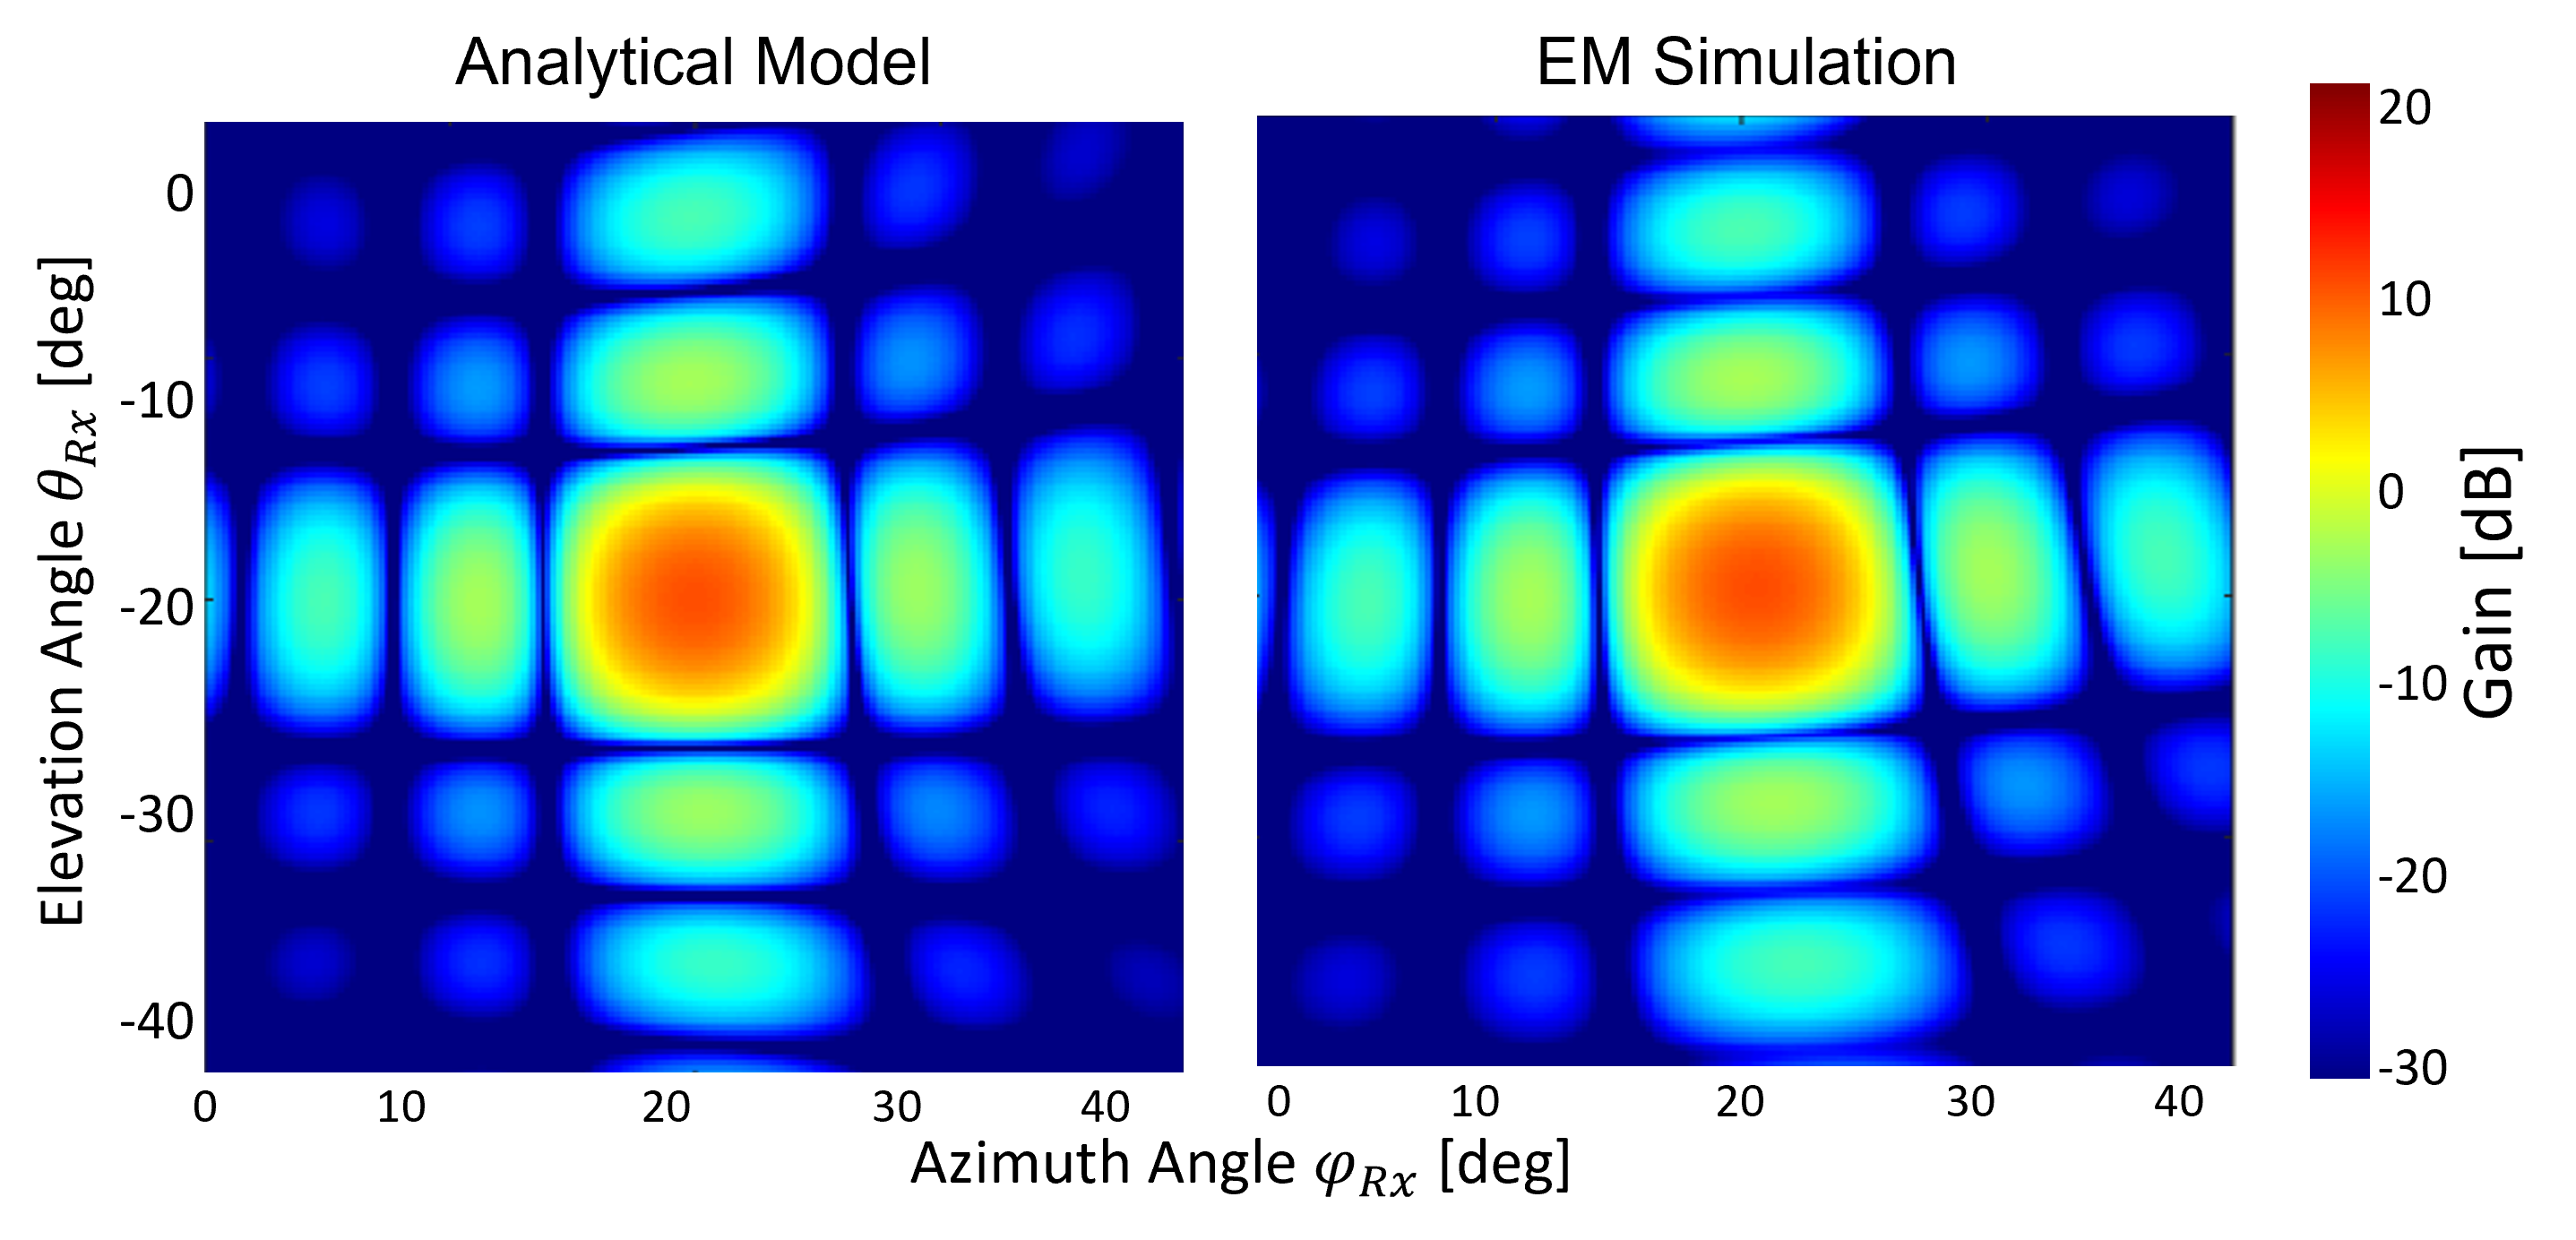
\includegraphics[width=0.82\linewidth]{images/Section 3 Images/Heatmap_1D}
	\caption{Sample RCS pattern of individual HELIOS module ($1 \times 1$): (left) analytical model, (right) EM simulations for parameters $a=b=\SI{10}{\centi\meter}$ and $\alpha=\beta=\num{10}^\circ$ at \SI{28}{\giga\hertz} frequency with peak gain of \SI{10.4}{\decibel}.}
	\label{fig:heatmap1d}
\end{figure}
Further adaptation of the HELIOS reflector module at \SI{38}{\giga\hertz} frequency is seen in \Cref{fig:heatmap_38GHz}. The peak gain by the analytical model and EM simulation results at \SI{28}{\giga\hertz} frequency is around \SI{10.4}{\decibel}, whereas at \SI{38}{\giga\hertz} frequency is \SI{13.0}{\decibel}. Because of their shorter wavelengths, reflectors typically show better gain characteristics at higher frequencies, such as \SI{38}{\giga\hertz}, allowing for more directed and focused signal propagation. This variant highlights how carrier frequencies and reflector performance interact intricately in 5G mmWave scenarios, impacting the network's overall signal propagation and coverage properties.
\begin{figure}[H]
	\centering
	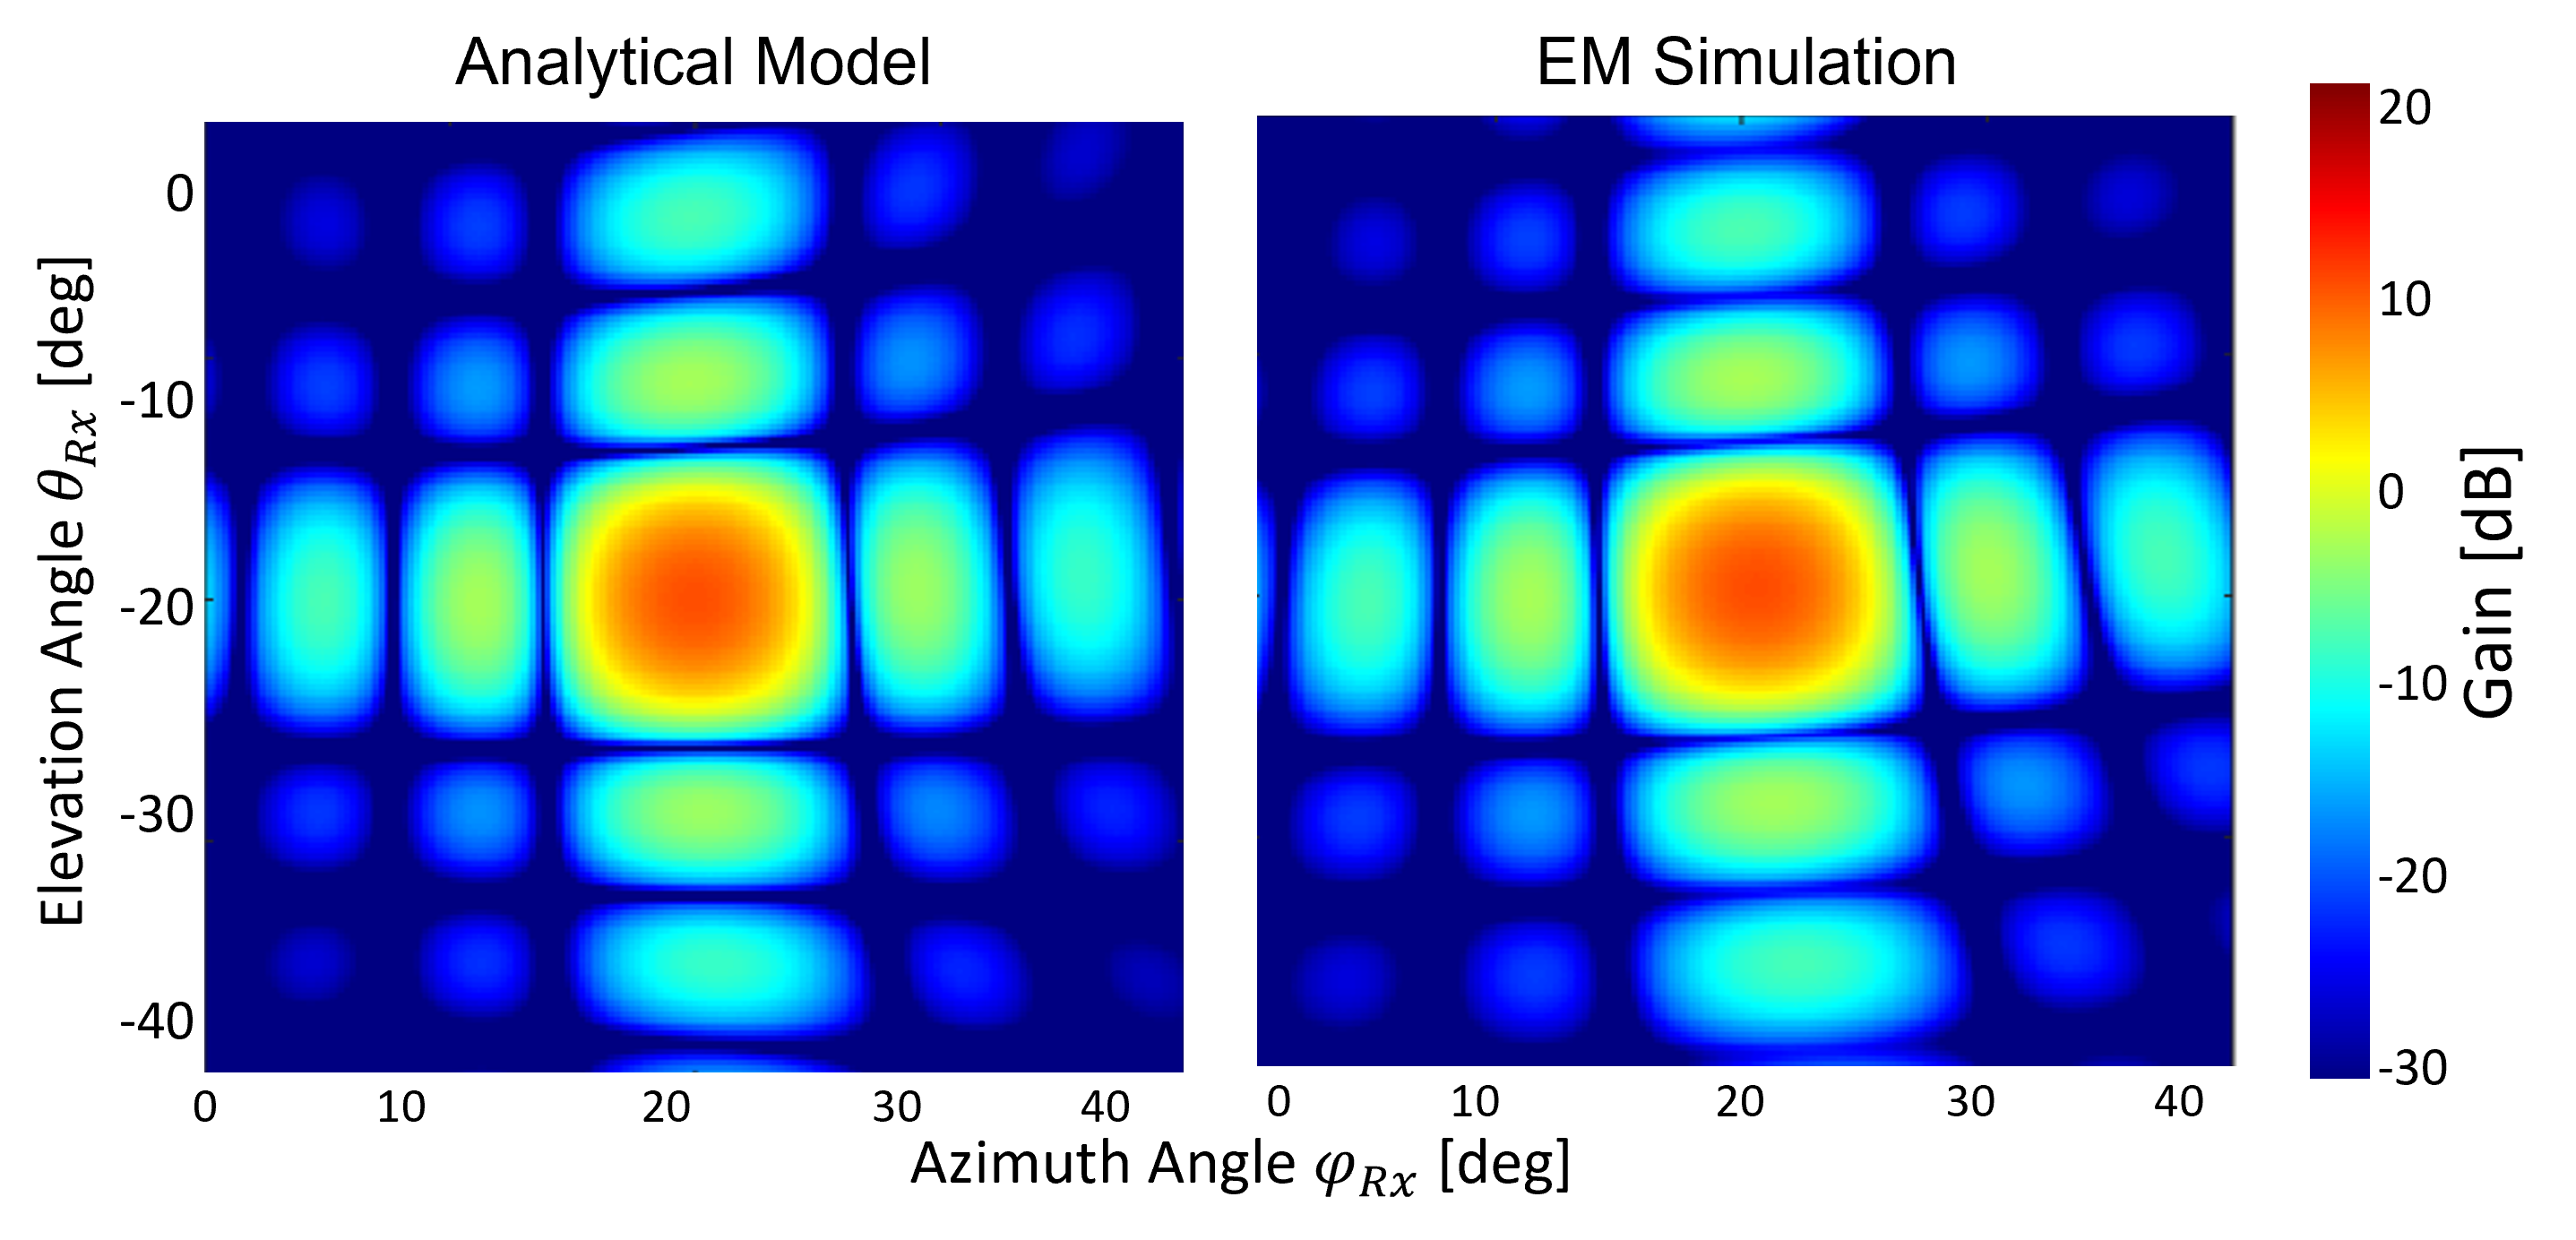
\includegraphics[width=0.82\linewidth]{images/Section 3 Images/Heatmap_1D}
	\caption{Sample RCS pattern of individual HELIOS module ($1 \times 1$): (left) analytical model, (right) EM simulations for parameters $a=b=\SI{10}{\centi\meter}$ and $\alpha=\beta=\num{10}^\circ$ at \SI{38}{\giga\hertz} frequency with peak gain of \SI{13.0}{\decibel}.}
	\label{fig:heatmap_38GHz}
\end{figure}
\section{Analytical Model for Multi-Module HELIOS Reflectors} \label{Simulation and Modeling of HELIOS Reflectors}
In this section, we now focus on HELIOS reflectors in the form of an array of HELIOS modules. Owing to this, our model from \Cref{Analytical Modeling of HELIOS Modules} is extended and subsequently reevaluated. An initial extension is carried out in \Cref{Independent Composition of Overall Reflection Characteristics}, after which the accuracy model is thoroughly assessed by looking at three case studies. The discussion of self-shadowing issues that could surface between certain selected modules of a reflector's modules is then covered in \Cref{Improved Model using Inter-module Relations}, depending on how it is configured. This concentrated examination seeks to improve the accuracy of the analytical model that is introduced in this thesis, guaranteeing a thorough comprehension and improvement of its functions.
\subsection{Independent Superposition of Overall Reflection Characteristics} \label{Independent Composition of Overall Reflection Characteristics}
The independent composition of overall reflection properties entails combining many separate HELIOS modules to realize fully-fledged reflectors or arbitrary characteristics. Thus, depending on a single, monolithic reflector, which has limitations, this modular approach provides a great degree of flexibility and adaptability. The established formula shown in \Cref{Eq:RCS_SUMMATION} allows for the superposition of the individual RCS patterns of the HELIOS module, thereby providing a formula for the overall HELIOS reflector array. Whereas one could use the bistatic RCS pattern from \Cref{Analytical Modeling of HELIOS Modules}, cf. \Cref{Eq:HELIOS_module}, we propose a minor variation in the form of factors $M/2$ and $N/2$ (inside the $\sinc$ function) considering the overall number of modules along $y$- and $z$-axes, see \Cref{Eq:HELIOS_array}.

The below equations describe the HELIOS reflector array as a whole, and it provides a baseline for comparing different configured models' RCS behavior. Notably, the beamwidth factor is influenced by the factors $M/2$ and $N/2$ in the equation. This parameter was successfully applied to a single HELIOS module with factors of $1/2$ each, see \Cref{Eq:HELIOS_module}.
\begin{equation}\label{Eq:RCS_SUMMATION}
	\sigma_{Array}= \left(\sum_{n=1}^{N}\sum_{m=1}^{M} \sqrt{\sigma_{module} \left( a_{m,n}, b_{m,n}, \alpha_{m,n}, \beta_{m,n} \right) } \right)^2,
\end{equation}
with
\begin{equation} \label{Eq:HELIOS_array}
	\footnotesize
	\begin{aligned}
		 \sigma_{module} &=4 \cdot \pi \cdot \Gamma \cdot \left( \frac{\left( a_{m,n}\sqrt{1+\tan^2(\alpha_{m,n})}\right) \cdot \left( b_{m,n} \sqrt{1+\tan^2(\beta_{m,n})} \right) }{\lambda} \right) ^2\\
		&\left( \cos^2 \left( \theta_{Tx}-\beta_{m,n} \right) \cdot \cos^2 \left( \theta_{Rx}-\beta_{m,n} \right) \cdot \cos^2 \left( \varphi_{Rx}-\alpha_{m,n} \right) \right)\\
		& \left( \sinc \left( \frac{M}{2} \cdot k \cdot b_{m,n} \sqrt{1+\tan^2(\beta_{m,n})} \cdot \left( \sin \left( \theta_{Rx}-\beta_{m,n} \right) \cdot \cos \left( \varphi_{Rx}-\alpha_{m,n} \right) -\sin \left( \theta_{Tx}-\beta_{m,n} \right) \cdot \cos \left( \varphi_{Tx}-\alpha_{m,n} \right) \right) \right) \right)^2\\
		&  \left( \sinc \left( \frac{N}{2} \cdot k \cdot a_{m,n} \sqrt{1+\tan^2(\alpha_{m,n})} \cdot \left( \cos \left( \theta_{Rx}-\beta_{m,n} \right) \cdot \sin \left( \varphi_{Rx}-\alpha_{m,n} \right) -\cos \left( \theta_{Tx}-\beta_{m,n} \right) \cdot \sin \left( \varphi_{Tx}-\alpha_{m,n} \right) \right) \right) \right)^2 
	\end{aligned}
\end{equation}

Three in-depth case studies are conducted to validate this equation. In the first investigation, RCS patterns from various setups are compared. An ECDF comparison between the analytical model and EM simulation results of the HELIOS reflector array is carried out in the second study. The third study provides a comprehensive analysis of the equation's performance in various settings by examining various configurations and sensible beamwidth factors. Together, these case studies advance our understanding of the RCS behavior and the versatility of the equation in various reflector array configurations.
\subsubsection{Case Study 1: RCS Pattern Comparison for Different HELIOS Configurations}
For validation of \Cref{Eq:HELIOS_array}, we study the peak RCS gains of different dimensions of HELIOS arrays in \Cref{fig:arraymax}. In particular, we examined arrays with dimensions of $\num{1}\times N$ and $M\times N$, where $M$ and $N$ are integers between \num{1} and \num{8}. Whereas, there is already a noteworthy degree of consistency, there are nonetheless differences against the simulation results. For example, for the $\num{1}\times \num{8}$ array depicted on the left side, there is a difference of about \SI{0.4}{\decibel} between the EM simulation results and our analytical model. If we consider the $\num{8}\times \num{8}$ array on the right side, the difference increases to a more noticeable \SI{1.2}{\decibel}. As we show in \Cref{Improved Model using Inter-module Relations}, this is due to self-shadowing between the individual HELIOS modules.

A thorough bistatic RCS heatmap comparison for $\num{2}\times \num{2}$, $\num{4}\times \num{4}$, and $\num{8}\times \num{8}$ HELIOS reflectors arrays is carried out to analyze the various analytical and simulation findings, where we observe a match in the behavior, as shown in \Cref{fig:heatmaparraz}. Interestingly, a pattern emerges from the observations: both the simulative and analytical model beams show a notable narrowing effect with increasing gains as the reflector footprint grows.
\begin{figure}[H]
	\centering
	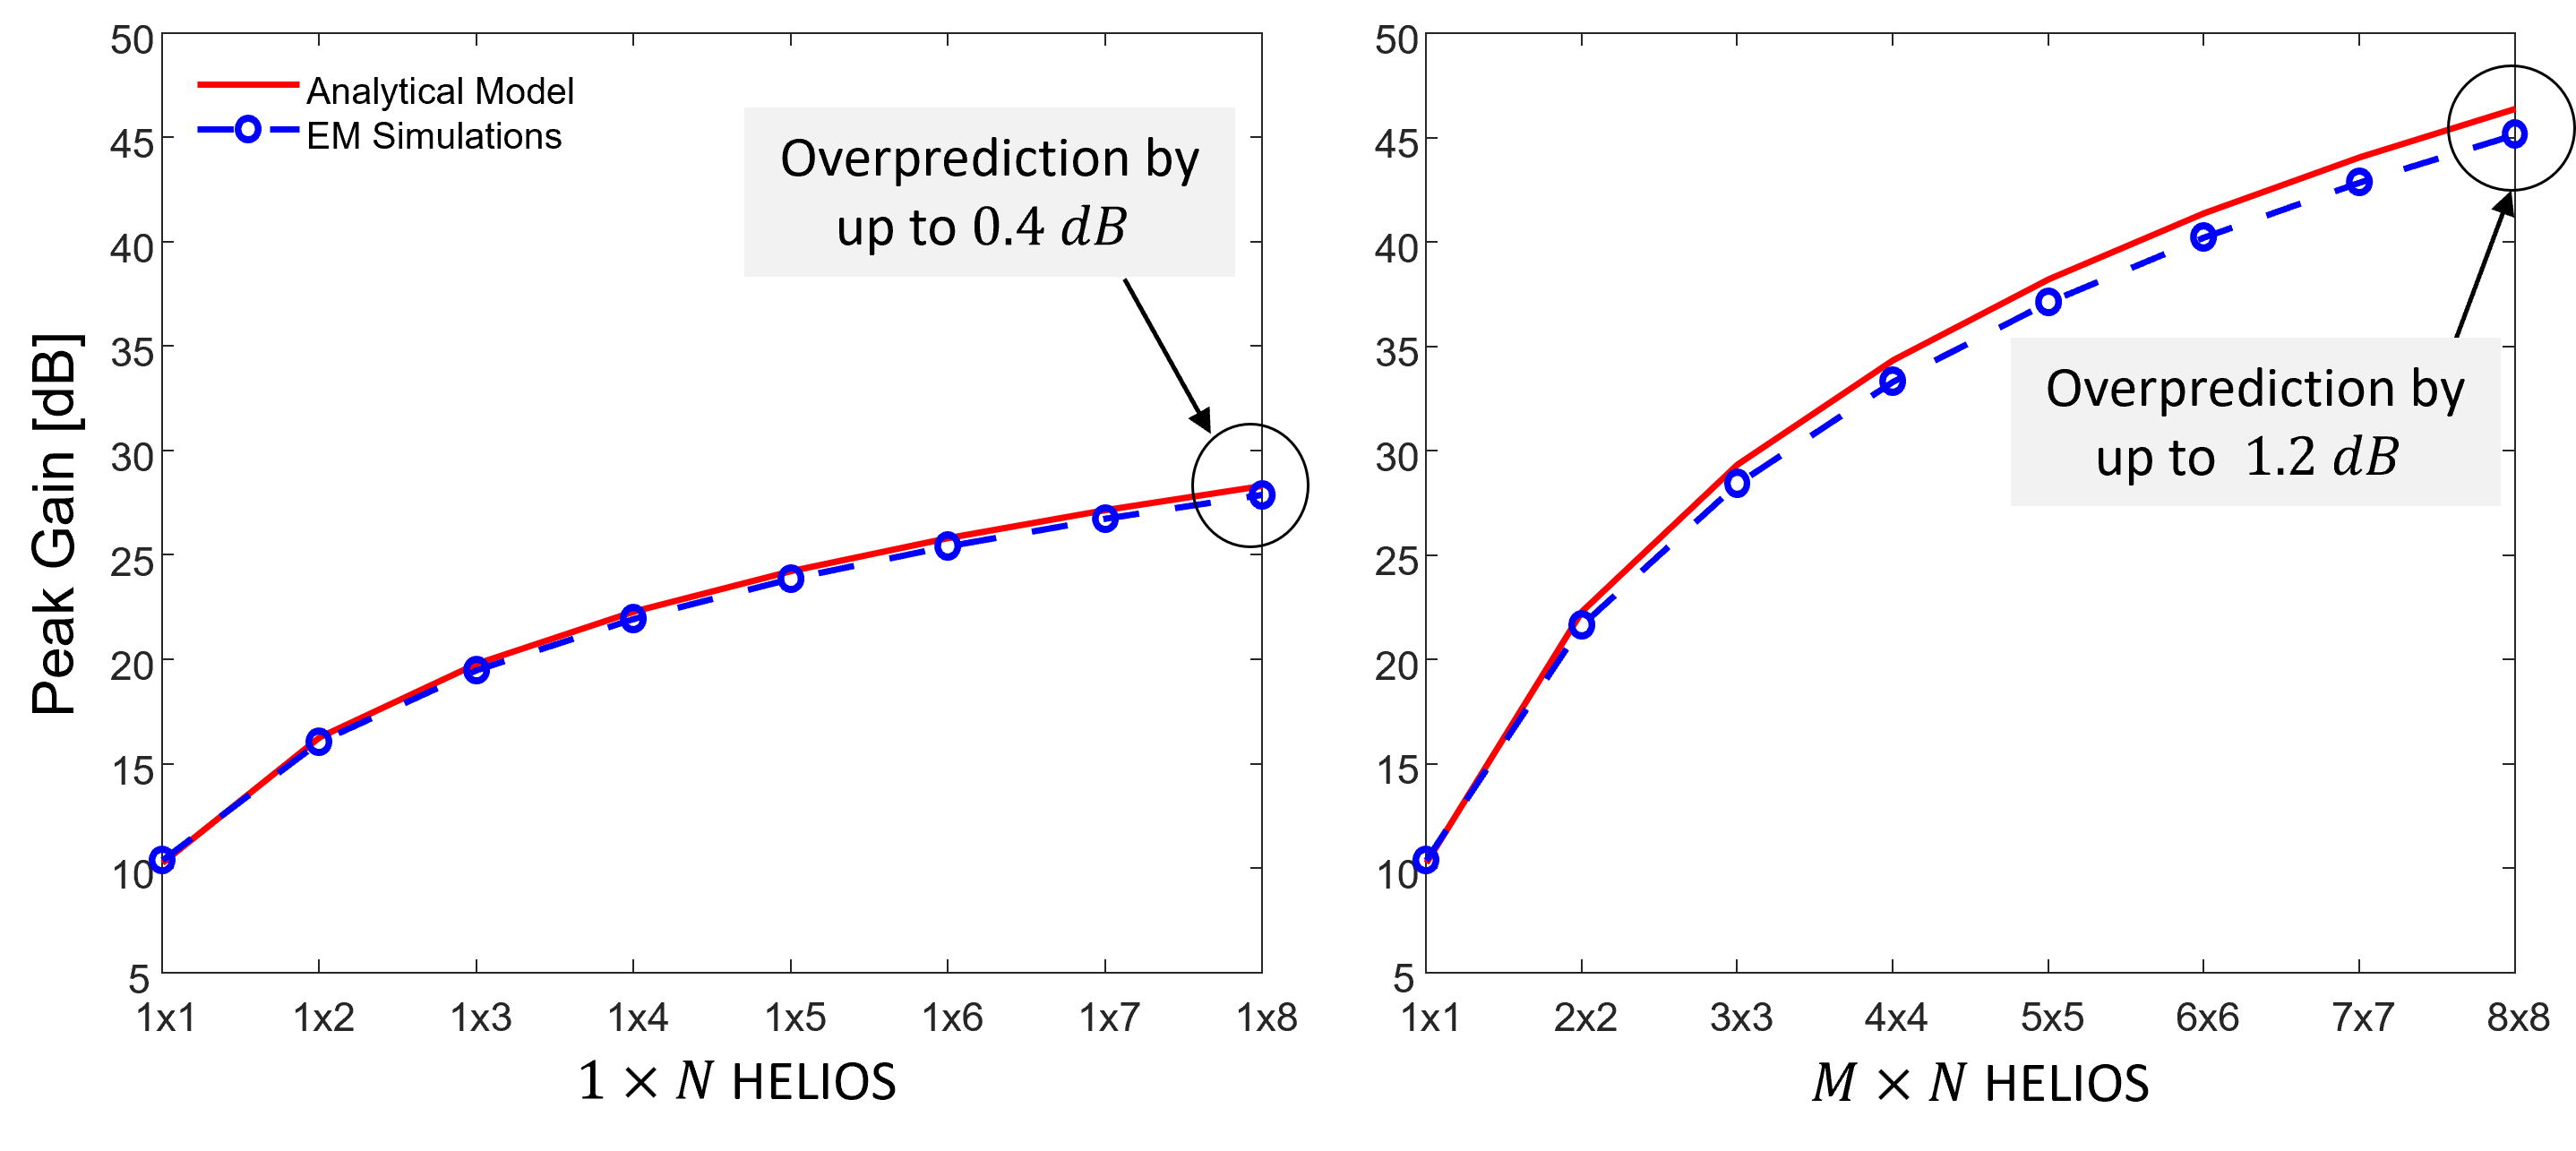
\includegraphics[width=1.0\linewidth]{images/Section 3 Images/Array_max}
	\caption{Plot against HELIOS array and maximum gain between simulated and analytical model highlighting the difference in gain in $\si{\decibel}$ for the case when $\alpha_{m,n}=\beta_{m,n}=10^\circ$ and $a_{m,n}=b_{m,n}= \SI{10}{\centi\meter}$ for $M=N\in[1:8]$ at \SI{28}{\giga\hertz} frequency.}
	\label{fig:arraymax}
\end{figure}
\begin{figure}[tb]
	\centering
	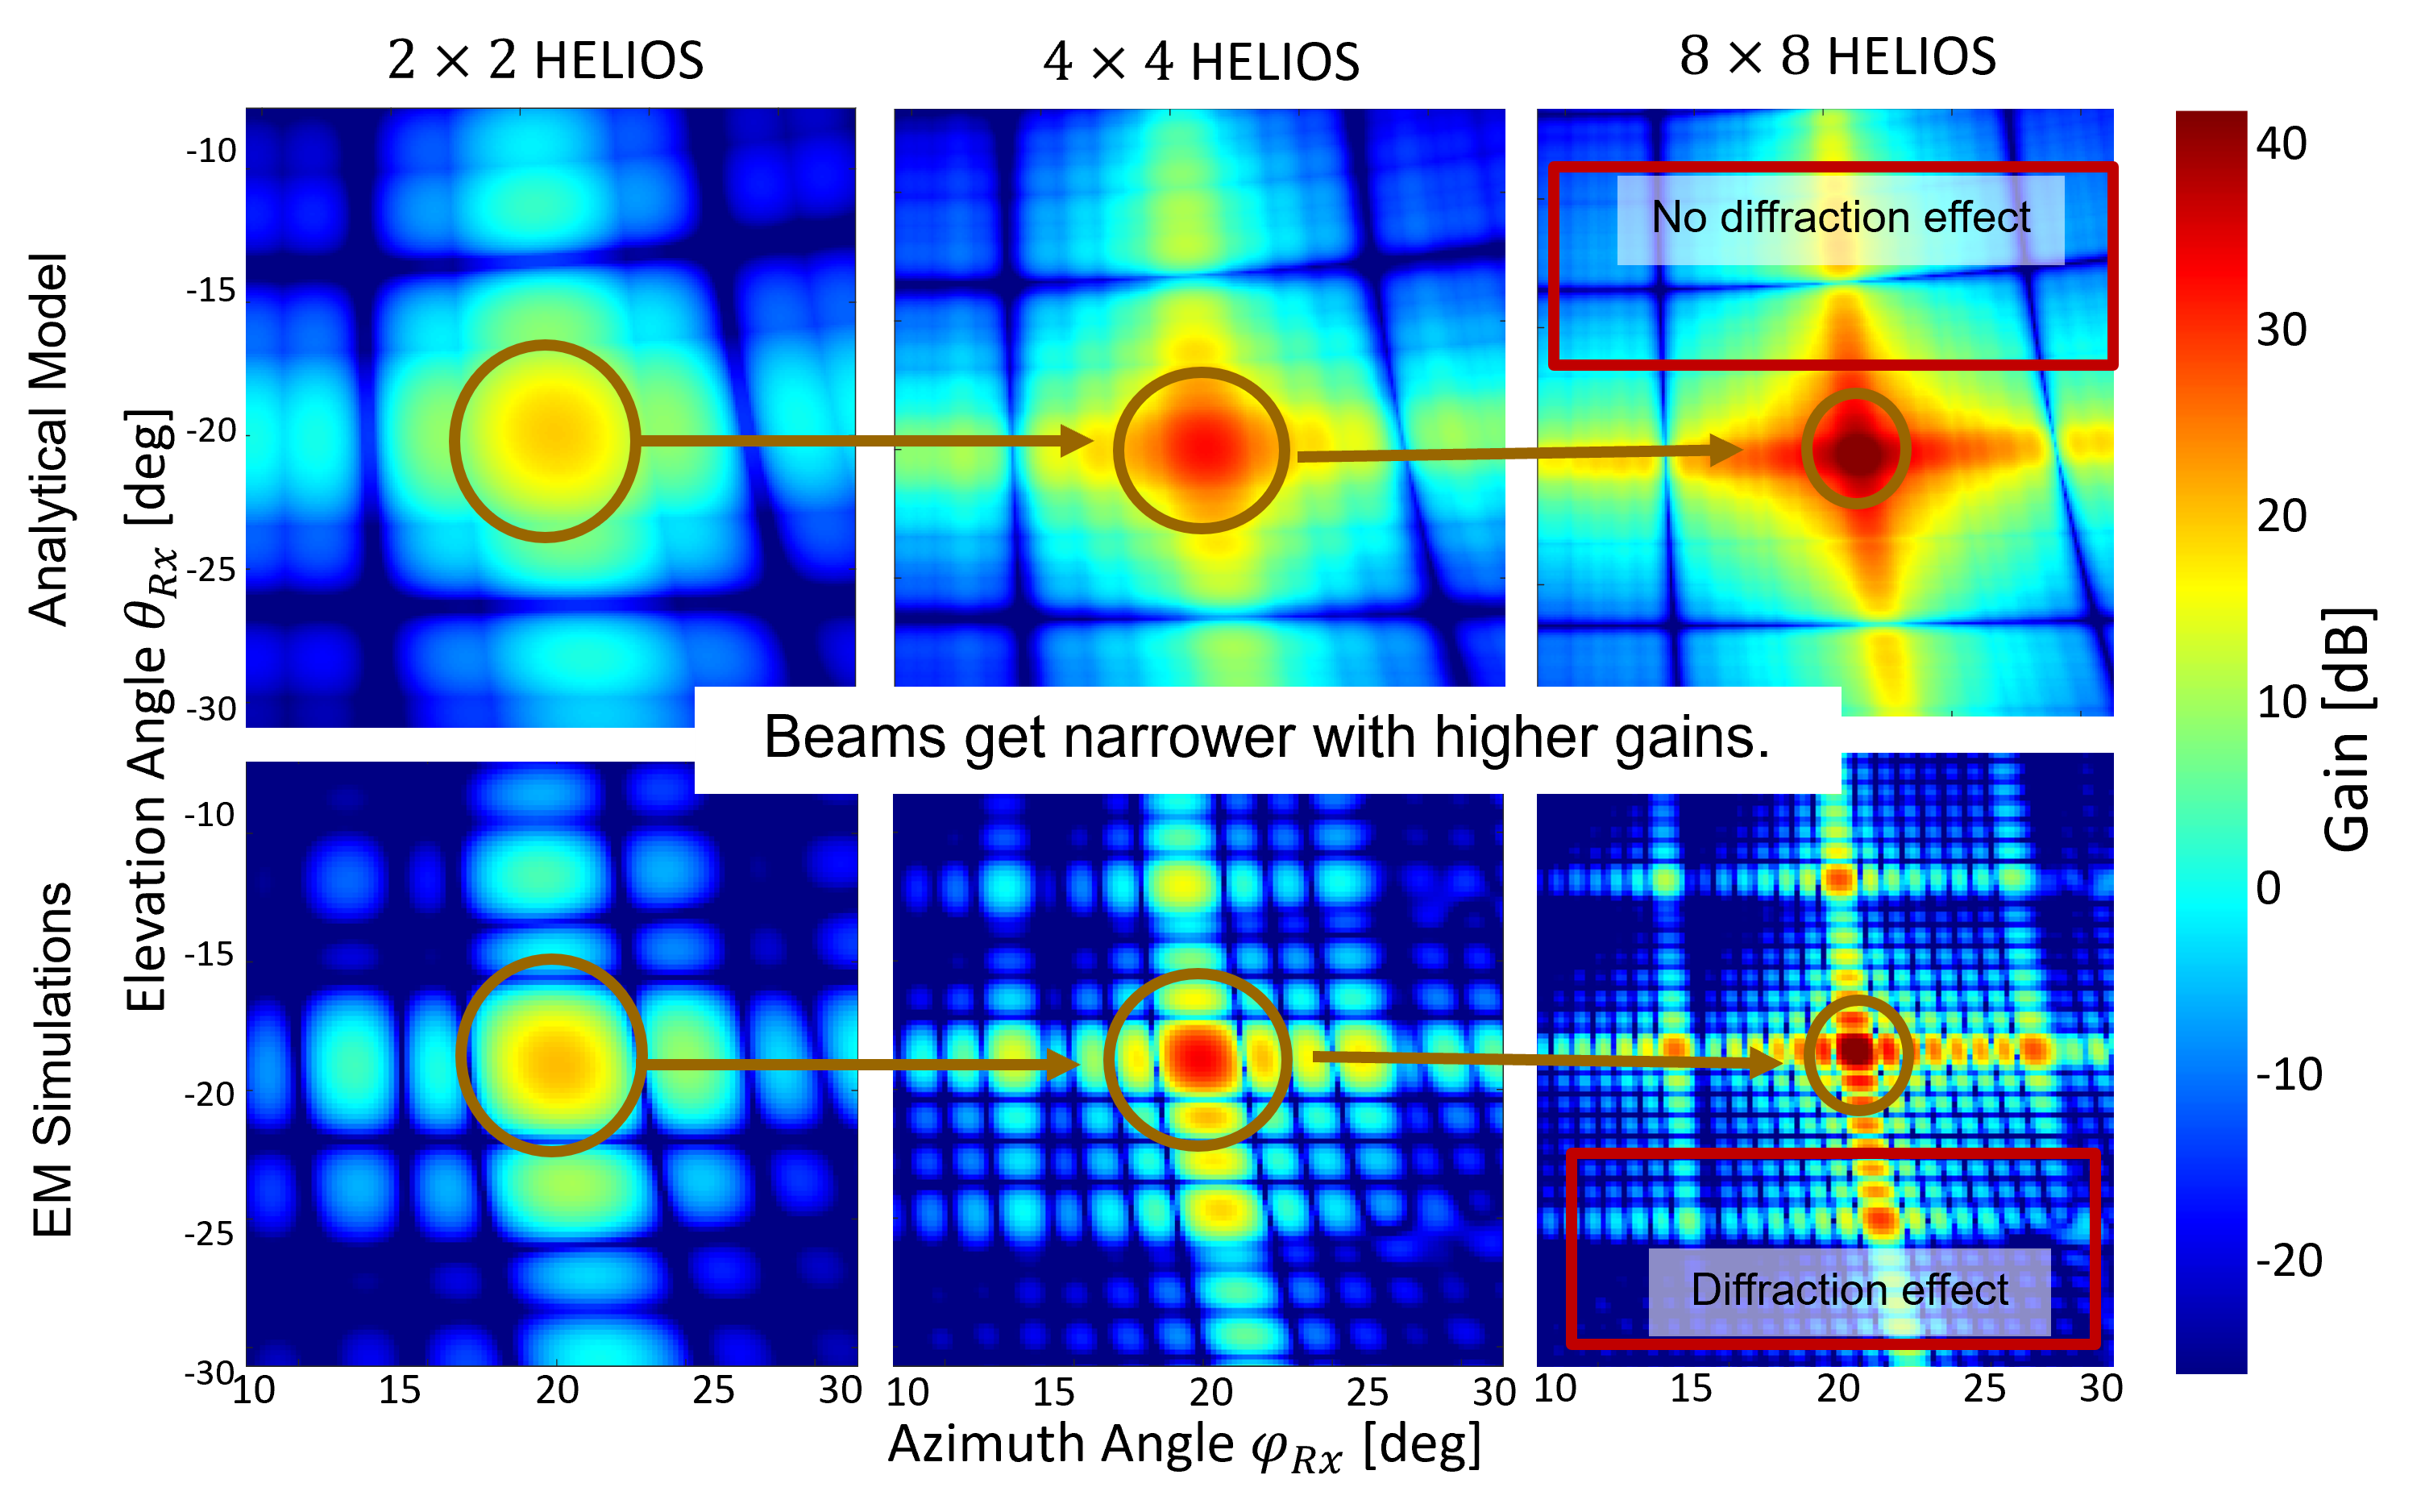
\includegraphics[width=1.0\linewidth]{images/Section 3 Images/Heatmap_arraz}
	\caption{RCS pattern behavior of HELIOS reflectors with different number of modules for simulation and analytical model highlighting the similarities in gains and beam patterns without the consideration of diffraction effect for $\alpha_{m,n}=\beta_{m,n}=10^\circ$ and $a_{m,n}=b_{m,n}= \SI{10}{\centi\meter}$. }
	\label{fig:heatmaparraz}
\end{figure}
Extending our analysis beyond the main lobe, we observe a limitation of our analytical model: diffraction effects are not included in the analytical model by default, as we are so far considering the models independently. This aspect can be addressed by future work. In the later part of this section, we refer to \Cref{Improved Model using Inter-module Relations} illustrates a similar fine-tuning of our model by considering inter-module shadowing effects.
\subsubsection{Case Study 2: ECDF Comparison of Analytical Model and EM Simulation Results for HELIOS Reflector Array.}
With an emphasis on both $\num{2}\times \num{2}$ and $\num{8}\times \num{8}$ HELIOS array configurations with $a_{m,n}=b_{m,n}=\SI{10}{\centi\meter}$, \Cref{fig:ECDF_HELIOS_array} depicts the ECDFs along the realized RCS gains which focuses on the performance differences between analytical and simulated values. As annotated in the plot, the more to the right the overall distribution curve is, the better the performance in terms of exhibited reflection power for the whole range of $\varphi_{Rx}$ and $\theta_{Rx}$ angles. The slope angles $\alpha_{m,n}=\beta_{m,n}=10^\circ$ with incident angles $\theta_{Tx}=\varphi_{Tx}=0^\circ$ at \SI{28}{\giga\hertz} frequency.

\begin{figure}[tb]
	\centering
	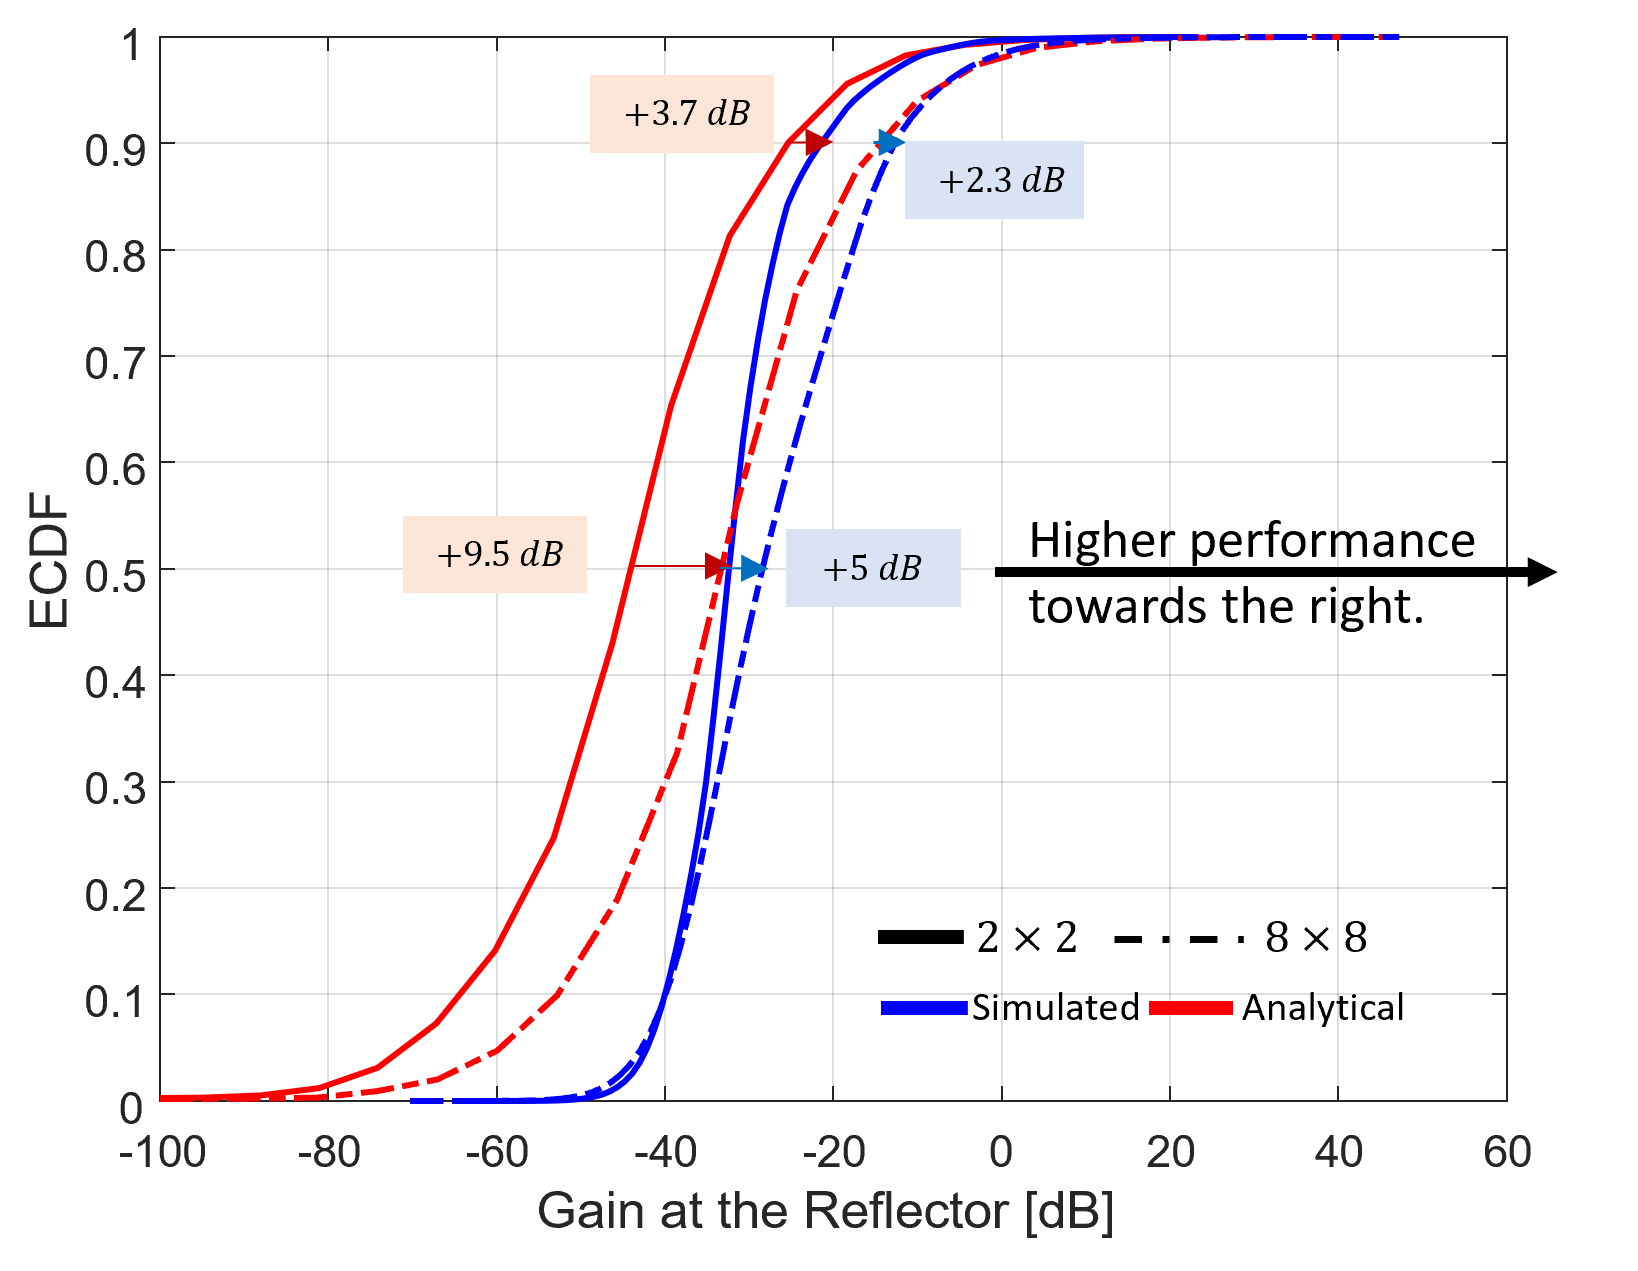
\includegraphics[width=0.7\linewidth]{images/Section 3 Images/ECDF_HELIOS_array}
	\caption{Gain vs ECDF plot for $\num{2}\times \num{2}$ and $\num{8}\times \num{8}$ HELIOS array with $a_{m,n}=b_{m,n}=\SI{10}{\centi\meter}$ for simulated and analytical results with a notable difference in gain between both the models when slope angles $\alpha_{m,n}=\beta_{m,n}=10^\circ$ with incident angles $\theta_{Tx}=\varphi_{Tx}=0^\circ$. }
	\label{fig:ECDF_HELIOS_array}
\end{figure}
Notably, for both types of HELIOS configurations, the simulation findings consistently show better performance than the analytical counterparts. Along the mean at $\num{2}\times \num{2}$ and $\num{8}\times \num{8}$ HELIOS array, the simulated results are better than the analytical model by \SI{9.5}{\decibel} and \SI{5}{\decibel} than the analytical model, whereas along the \num{90}\% quartile, the simulated results are better by \SI{3.7}{\decibel} and \SI{2.3}{\decibel}, respectively. The fact that the gain values are constantly lower shows that the analytical model avoids over-prediction. This discrepancy between the analytical and simulation results indicates a cautious approach because it suggests a conservative estimate in the analytical model. In practical applications, this careful prediction ensures that the actual performance of the system is less likely to deviate from the expected values, hence improving the analytical model's robustness and reliability. Network planning will now rather use too many reflectors or larger ones compared to not meeting the required target received signal strengths.
\subsubsection{Case Study 3: RCS Pattern Comparison for Different HELIOS Configurations and Beamwidth Factors}
The scalability needed by larger HELIOS reflectors is not met by applying \Cref{Eq:HELIOS_module} in the $\num{1}\times \num{1}$ HELIOS module. To find an ideal solution for the bigger reflector designs, we investigate and evaluate various beamwidth correction factors in order to overcome this constraint. 
One important finding from our analysis of the beamwidth correction factor for a HELIOS module is seen in \Cref{Eq:HELIOS_module} and \Cref{Table:Comparison flat plate and HELIOS}, where the correction factor is found to be $(\frac{1}{2},\frac{1}{2})$ for a HELIOS module. But when you move to an array configuration, you see a significant difference. To investigate this, we carried out a thorough analysis comprising multiple parameters, as shown in \Cref{fig:Casestudy_beamwidth} for a $\num{4}\times \num{4}$ array as well as a HELIOS module.

Referring to \Cref{Eq:HELIOS_array}, which is our final independent analytical model for the HELIOS reflector array, we vary $M/2$ and $N/2$ in both the $\sinc$ functions to change their beamwidth factor. These components include $(\frac{M}{2},\frac{N}{2})$, $(M,N)$, in addition to the previously mentioned $(\frac{1}{2},\frac{1}{2})$. 
\begin{figure}[tb]
	\centering
	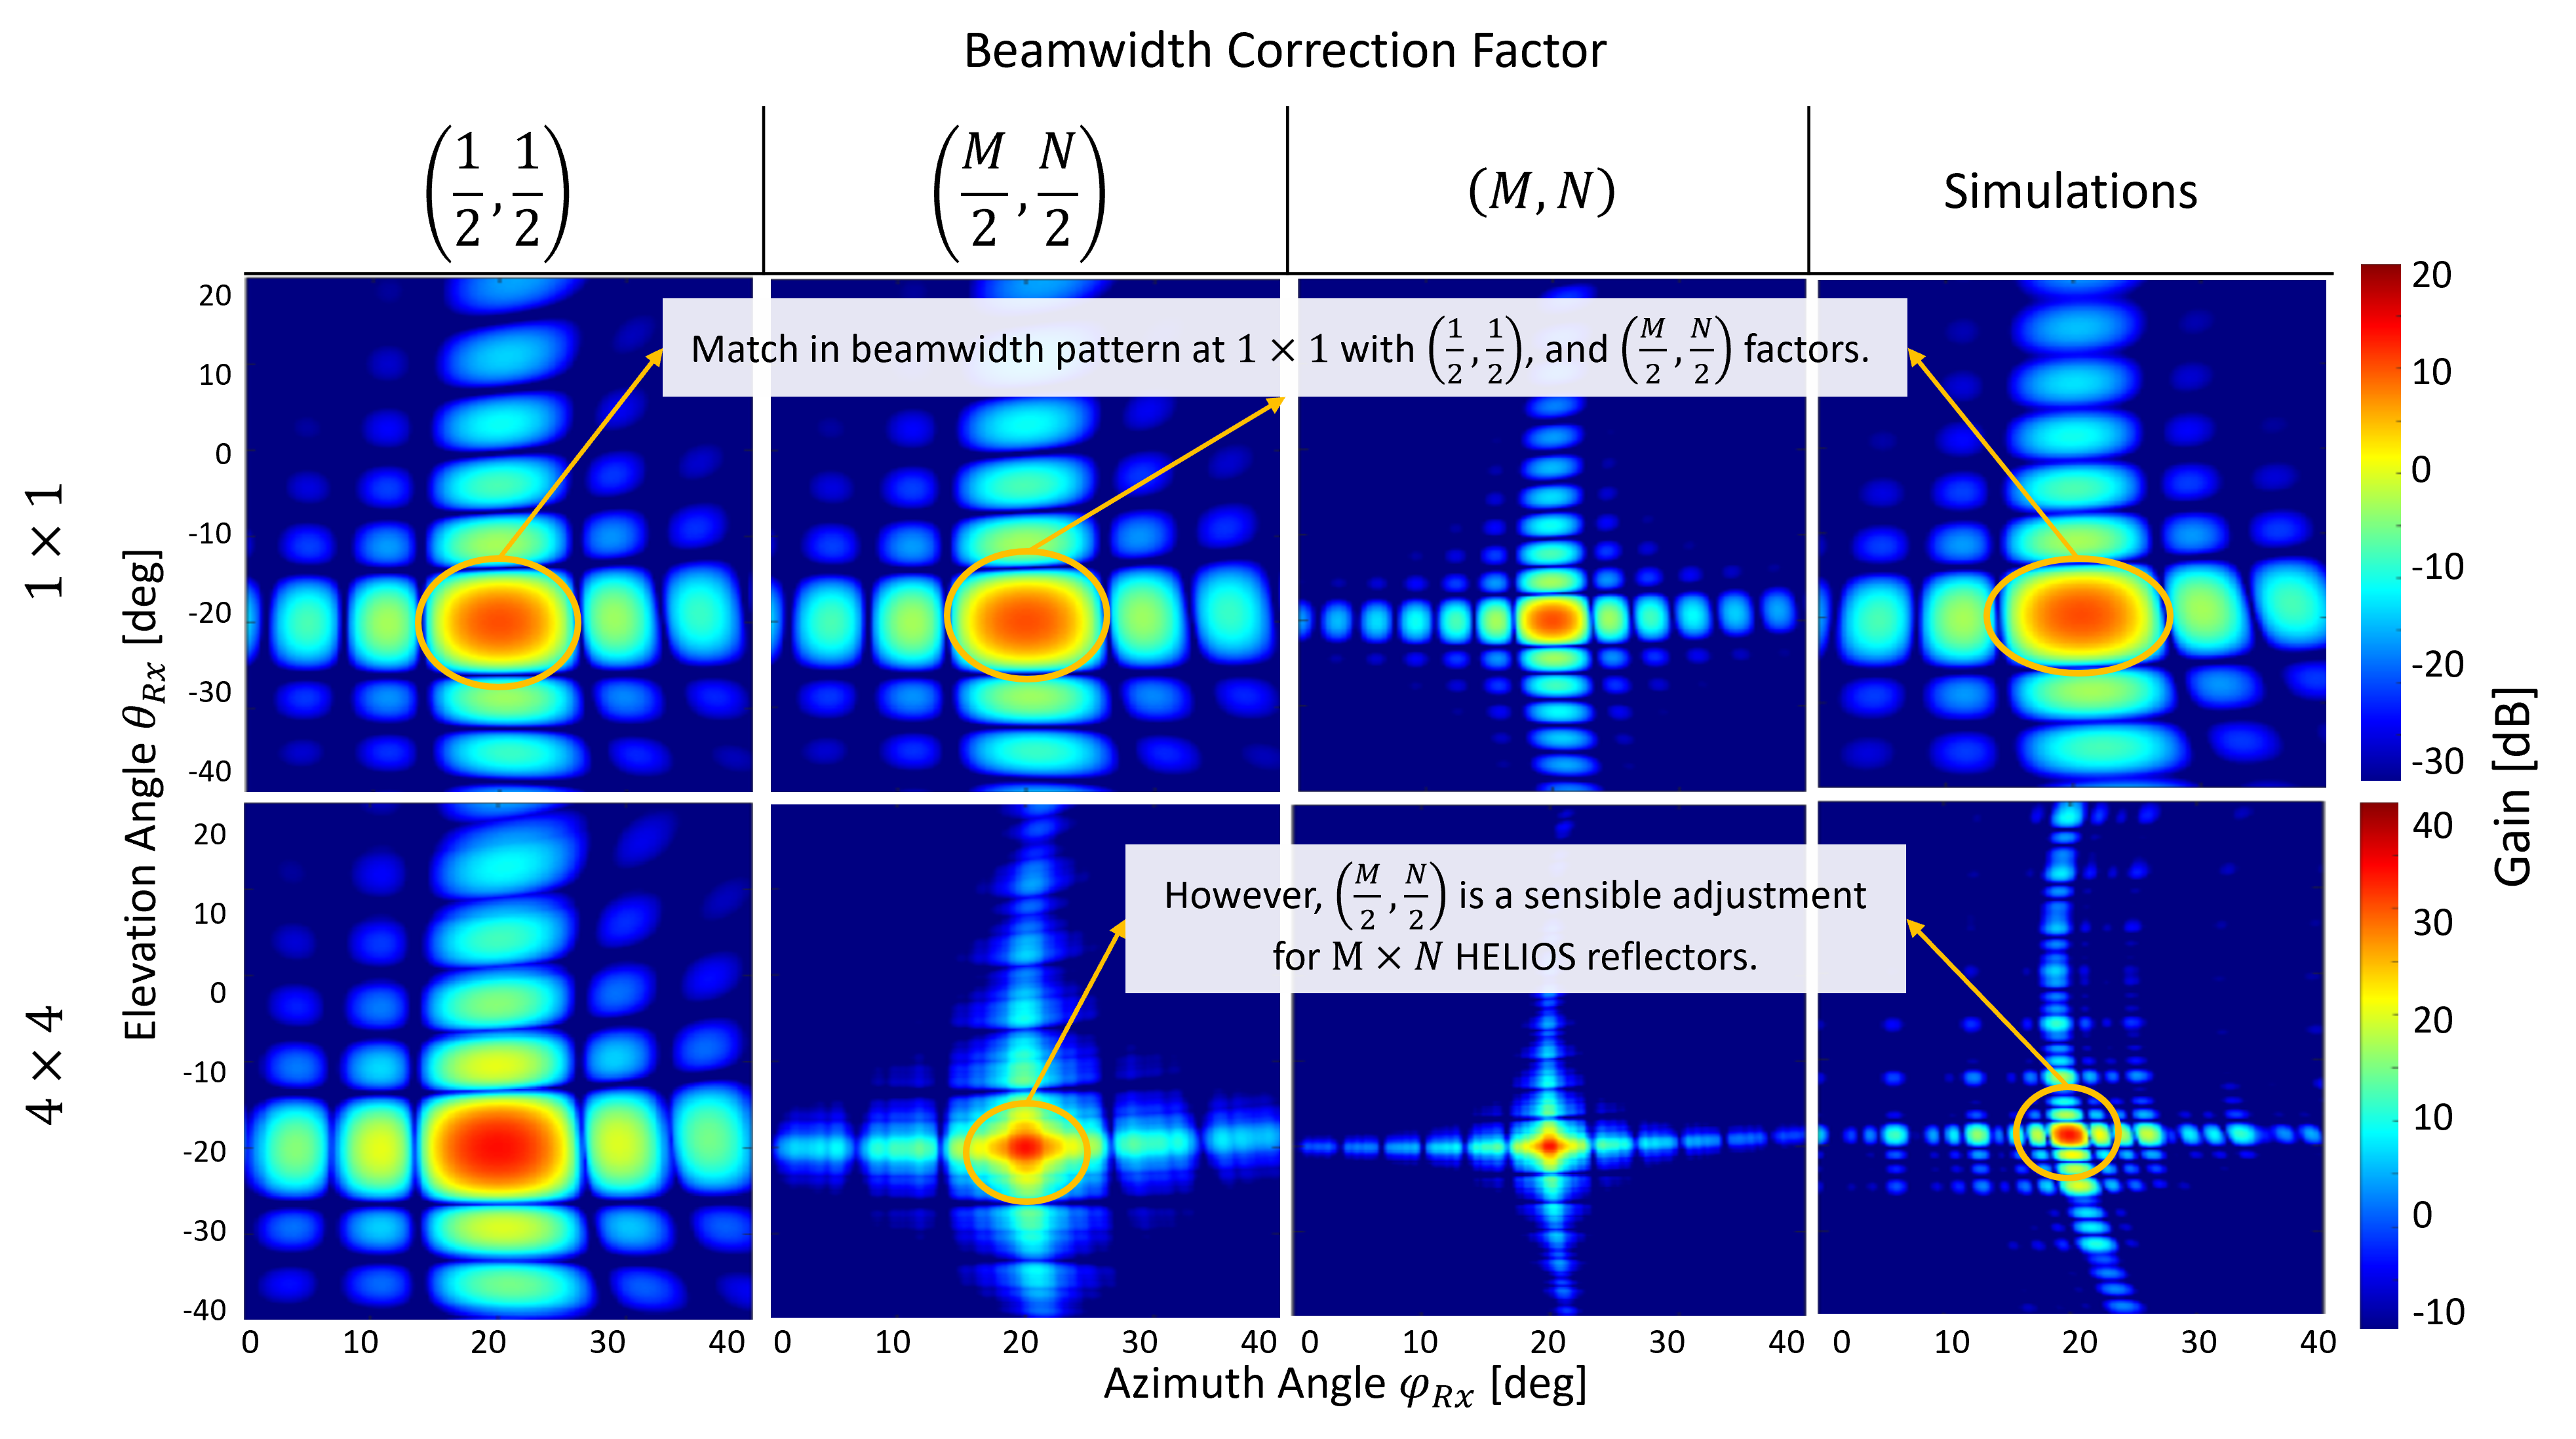
\includegraphics[width=1.0\linewidth]{images/Section 3 Images/Casestudy_beamwidth}
	\caption{Illustrating the RCS behavior of a HELIOS module and HELIOS array for different beamwidth correction factors in comparison with the simulated results when $\alpha_{m,n}=\beta_{m,n}=10^\circ$ and $a_{m,n}=b_{m,n}=\SI{10}{\centi\meter}$ for $M=N\in[1,4]$.}
	\label{fig:Casestudy_beamwidth}
\end{figure}
For the $\num{1}\times \num{1}$ and $\num{4}\times \num{4}$ HELIOS reflector array with $\alpha_{m,n}=\beta_{m,n}=10^\circ$, $a_{m,n}=b_{m,n}=\SI{10}{\centi\meter}$, and $\theta_{Tx}=\varphi_{Tx}=0^\circ$, we notice the RCS behavior in the form of heatmap in \Cref{fig:Casestudy_beamwidth}. The notable match is observed at $(\frac{M}{2},\frac{N}{2})$ and $(\frac{1}{2},\frac{1}{2})$ in the RCS heatmaps, but observing the behavior at $\num{4}\times \num{4}$ HELIOS reflector array, there's a sensible match at $(\frac{M}{2},\frac{N}{2})$.  We observe a better match in the results for larger arrays using  $(\frac{M}{2},\frac{N}{2})$ as the beamwidth correction factor.

In addition, we study a flat plate of fixed overall size by setting $\alpha_{m,n}=\beta_{m,n}=0^\circ$ with the incident wave impinging from $\theta_{Tx}=\varphi_{Tx}=0^\circ$. Like in the previous paragraph, we use the beamwidth correction factors of $(\frac{M}{2},\frac{N}{2})$, $(M,N)$, in addition to the previously mentioned $(\frac{1}{2},\frac{1}{2})$ from \Cref{Eq:HELIOS_module}. This is because we consider the same flatplate in the form of two different representations: First, as a large $\num{1}\times \num{1}$ HELIOS reflector with dimensions $a=\SI{40}{\centi\meter}$, and $b=\SI{10}{\centi\meter}$. Second, the overall plate shall be represented by four modules in the form of a $\num{1}\times \num{4}$ HELIOS with individual modules having the dimensions of $a_{m,n}=b_{m,n}=\SI{10}{\centi\meter}$. We compare the resulting overall bistatic RCS heatmaps in \Cref{fig:Casestudy_flatplate}.

In the figure below, for $1 \times 1$ large flat plate, we observe the match in the RCS heatmap behavior with beamwidth factor $(\frac{1}{2},\frac{1}{2})$, and $(\frac{M}{2},\frac{N}{2})$, whereas, for $1 \times 4$ small flat plates, the match can be observed only with beamwidth factor $(\frac{M}{2},\frac{N}{2})$. The same results were seen in \Cref{fig:Casestudy_beamwidth}, with $(\frac{M}{2},\frac{N}{2})$ as the sensible adjustment of beamwidth factor for HELIOS reflector array.
\begin{figure}[tb]
	\centering
	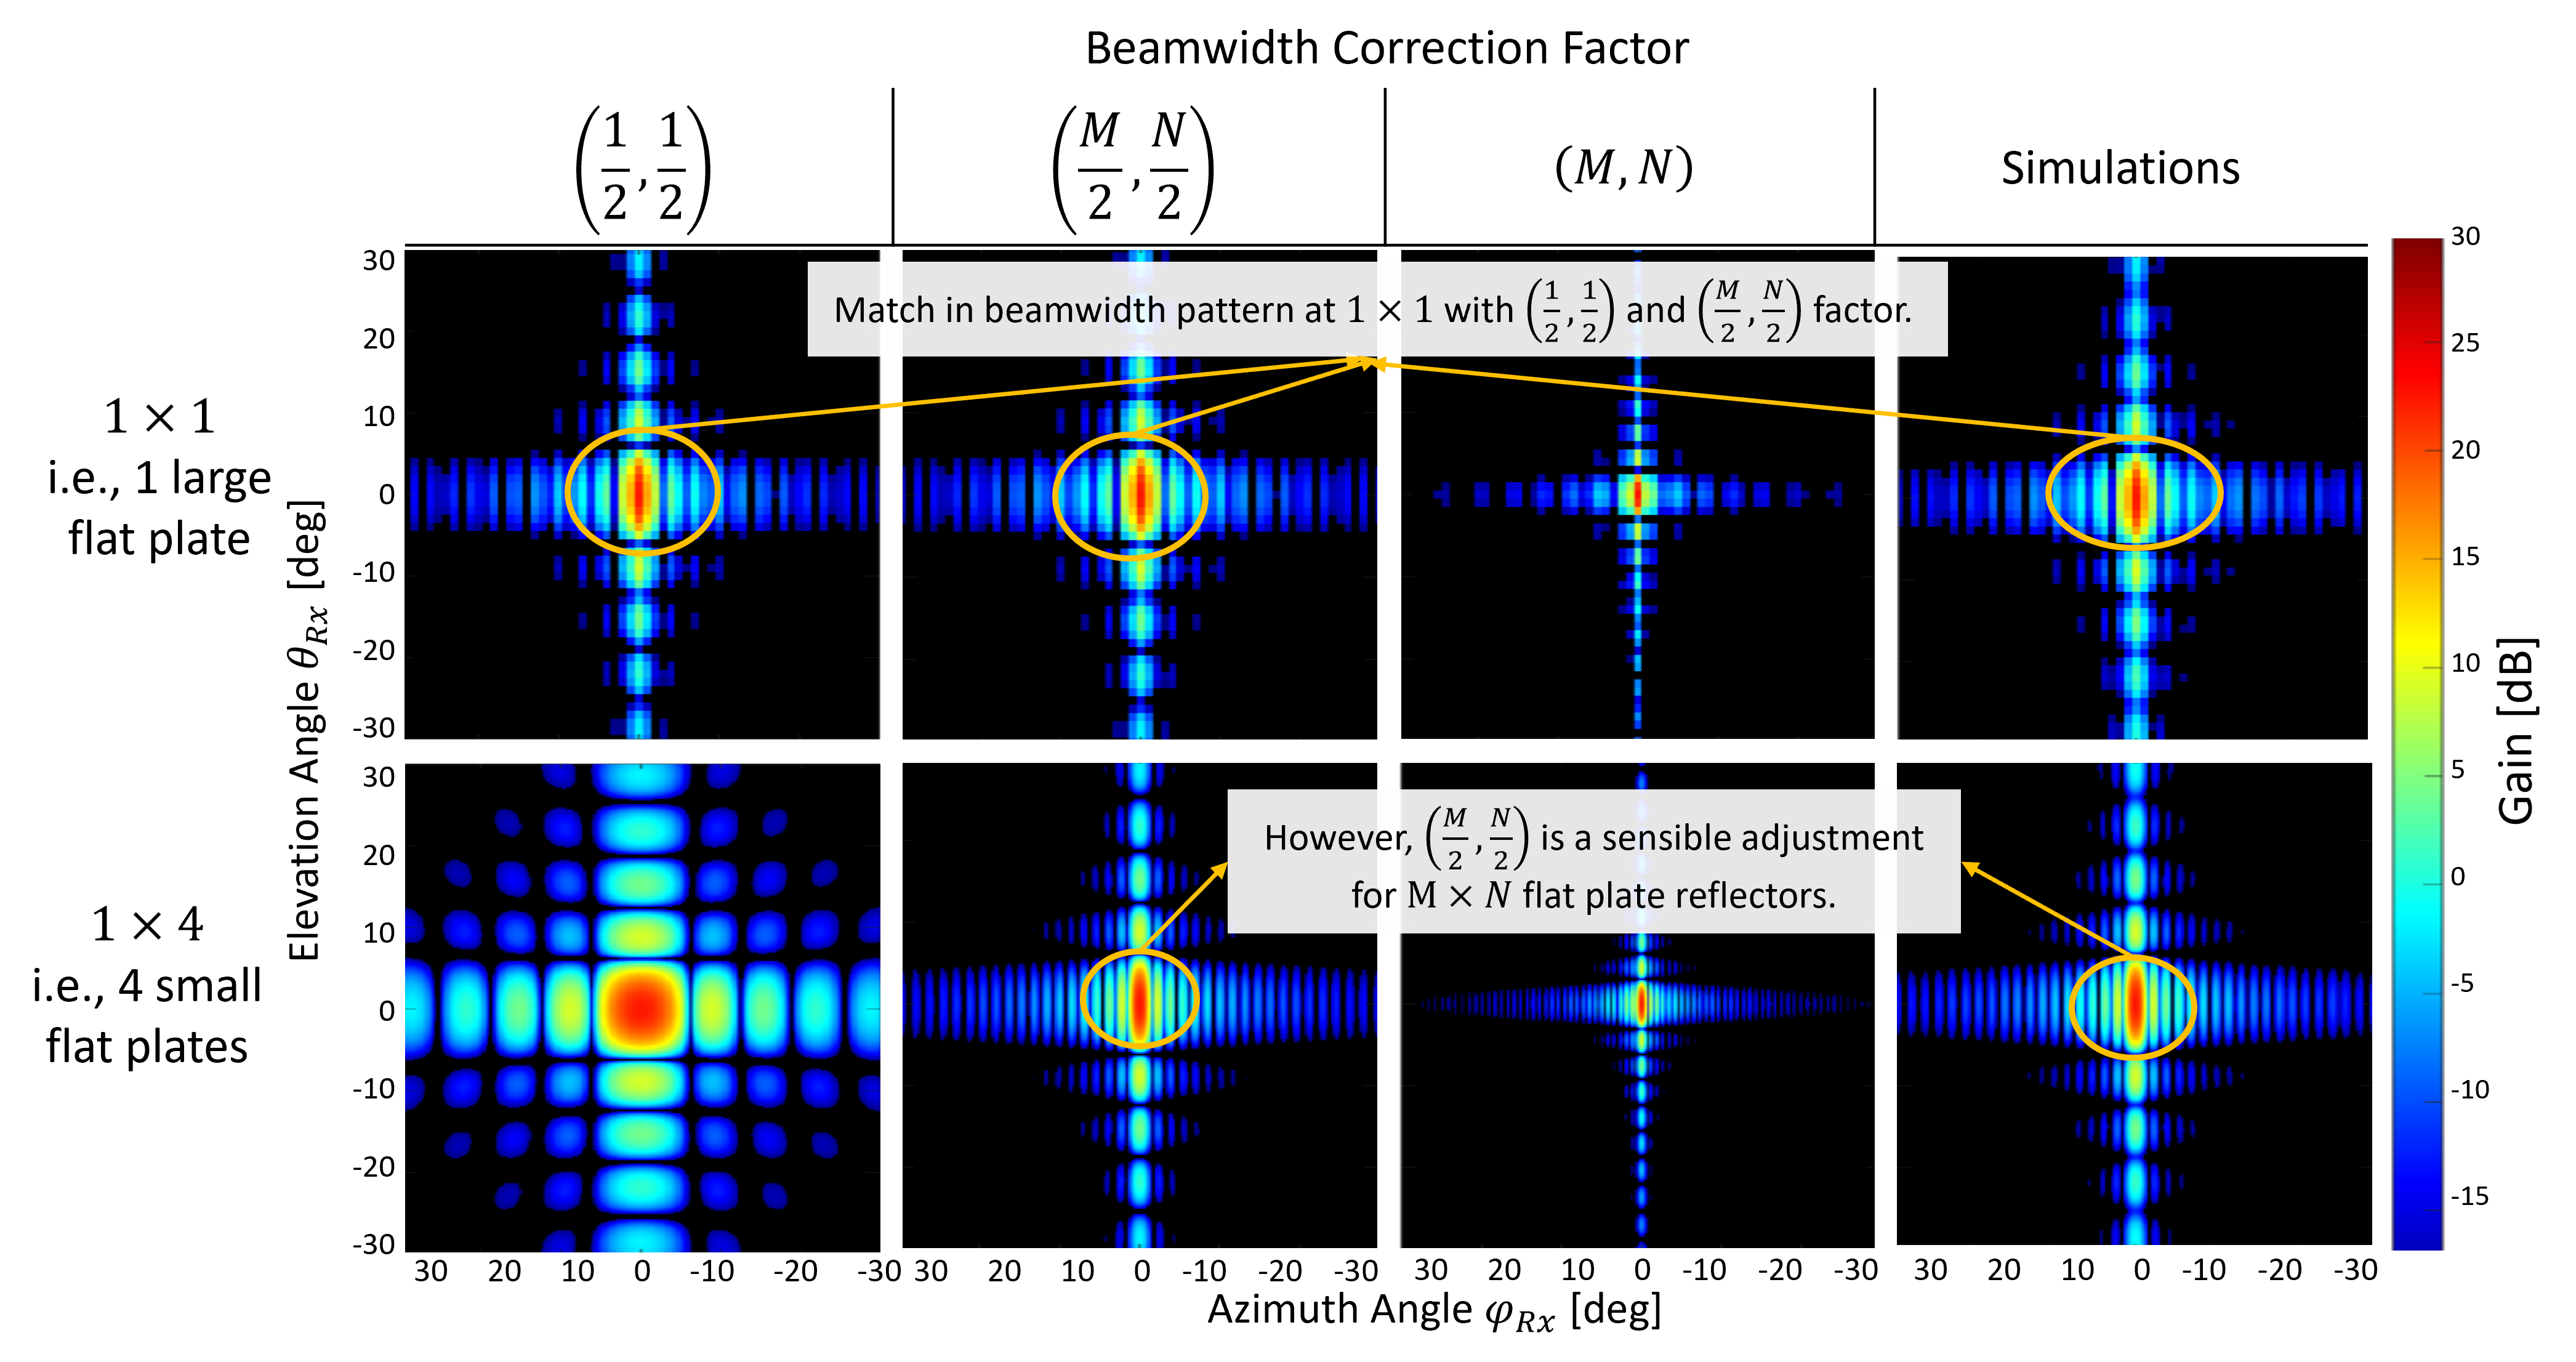
\includegraphics[width=1\linewidth]{images/Section 3 Images/Casestudy_flatplate}
	\caption{Illustrating the impact of different beamwidth correction factors in comparison with the simulations when $\alpha_{m,n}=\beta_{m,n}=0^\circ$ for a single big flat plate with $a_{m,n}=\SI{40}{\centi\meter}$, and $b_{m,n}=\SI{10}{\centi\meter}$ and multiple small flat plates with $a_{m,n}=b_{m,n}=\SI{10}{\centi\meter}$, where both the cases $1 \times 1$ and $1 \times 4$ represent the same physical plate. Notably, with beamwidth factor of $(\frac{1}{2},\frac{1}{2})$, and $(\frac{M}{2},\frac{N}{2})$, there's a match with the simulations at $1 \times 1$ , but at $1 \times 4$ HELIOS reflectors, the match is observed with beamwidth factor $(\frac{M}{2},\frac{N}{2})$.}
	\label{fig:Casestudy_flatplate}
\end{figure}
\begin{figure}[H]
	\centering
	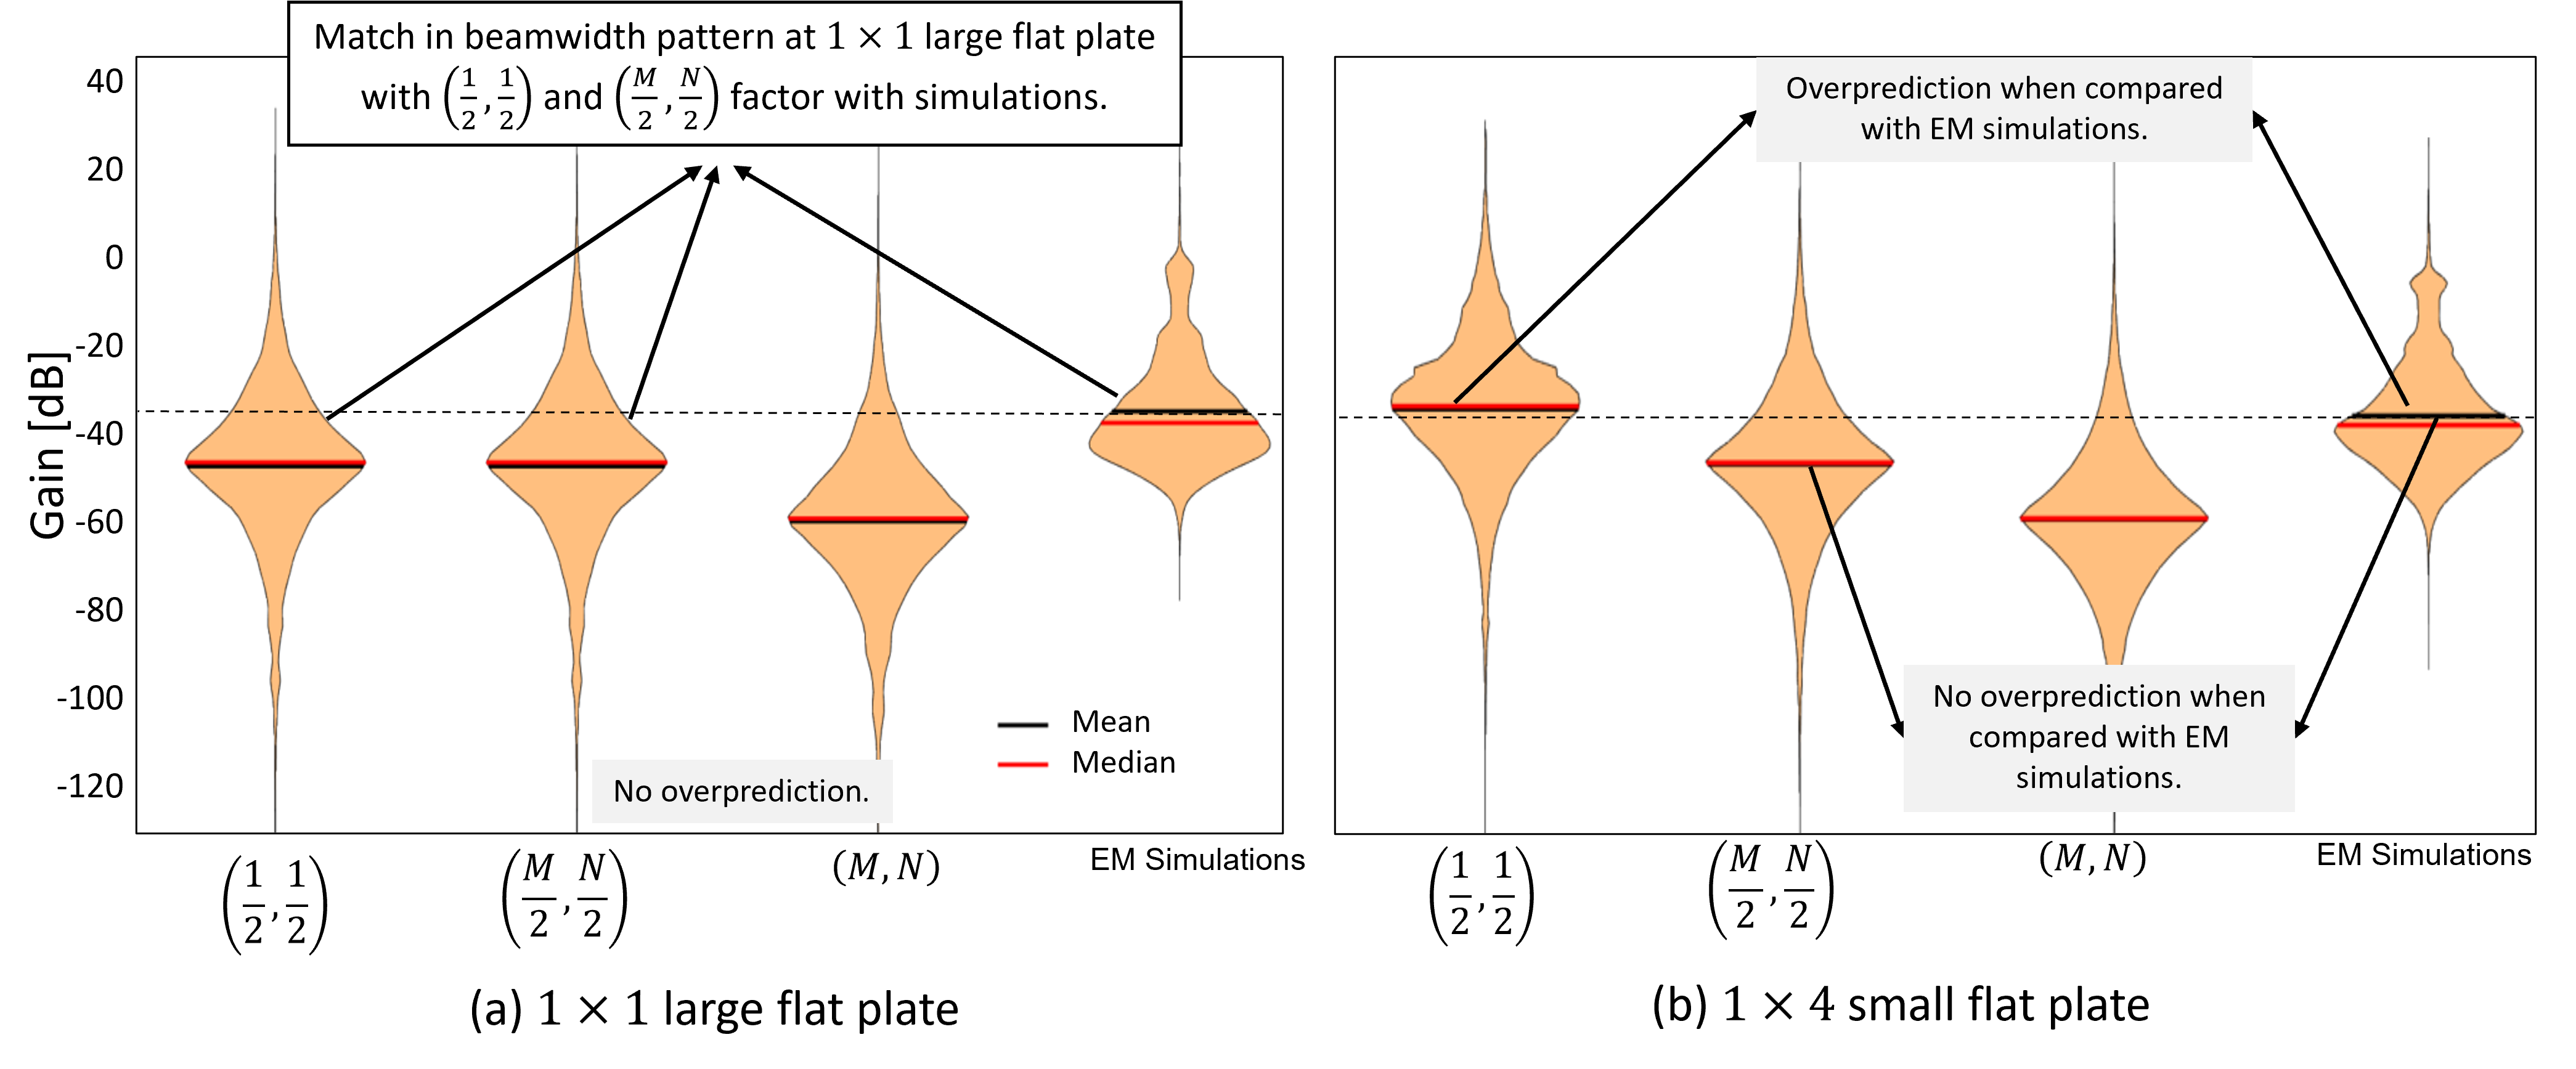
\includegraphics[width=1.0\linewidth]{images/Section 3 Images/Casestudy_flatplate_violin}
	\caption{Violin plot comparison for a flat plate scenario for different beamwidth correction factors. (a) A single big flat plate with $a_{m,n}=\SI{40}{\centi\meter}$, and $b_{m,n}=\SI{10}{\centi\meter}$, and a notable match with EM simulations with beamwidth factor of $(\frac{1}{2},\frac{1}{2})$, and $(\frac{M}{2},\frac{N}{2})$ with no overpredictions. (b) 4 small flat plates with $a_{m,n}=b_{m,n}=\SI{10}{\centi\meter}$ and a match with the simulations with beamwidth factor $(\frac{M}{2},\frac{N}{2})$ with no overpredictions. Both the cases $1 \times 1$ and $1 \times 4$ represent the same physical plate.}
	\label{fig:Casestudy_flatplate_violin}
\end{figure}
We also consider the above discussed RCS heatmaps in the form of violin plots, see \Cref{fig:Casestudy_flatplate_violin}. Notably, our analytical model regularly predicts slightly lower values, as evidenced by the mean and median values for beamwidth correction factors $(\frac{M}{2},\frac{N}{2})$, and $(M,N)$ falling below the corresponding simulation findings with both $1 \times 1$ large flat plate and $1 \times 4$ small flat plate. But when using the $(\frac{1}{2},\frac{1}{2})$ correction factor, this disparity is not seen in $1 \times 4$ small flat plate, as the model overpredicts when compared with EM simulations. Significantly, this actual data supports the analytical model and points to one of its positive features: it predicts values that are slightly lower than those obtained from simulations with beamwidth factor  $(\frac{M}{2},\frac{N}{2})$, which is in line with our intended results as argued previously.

The focus of this extended study is now to compare our analytical model with the EM simulations for a $1\times 32$ HELIOS reflector using different beamwidth correction factors. It is assumed that incidence angles are orthogonal to the backplane of the reflector, i.e., $\varphi_{Tx}=\theta_{Tx}=0^\circ$  with slope angles $\alpha_{1}=...\alpha_{32}=\num{27.6}^\circ$ and $\beta_{m,n}=0^\circ$. The overall size of the reflector shall be tuned by factor $K$ affecting the size along $y$-axis and $z$-axis, respectively, as follows: $a_{m,n}=K \cdot \frac{3}{32}$ and $b_{m,n}=K \cdot 3$ with $K = (0.1, 0.3, 0.5, 0.7)$, where $a_{m,n}$ and $b_{m,n}$ are in \si{\meter}.

\Cref{fig:Casestudy_orthogonal_BCF} provides a violin plots of $\Delta Gain$ (in \si{\decibel}) defined by $RCS_{Sim} - RCS_{Anal}$ in order to study the influence of reflector size and beamwidth correction factor on the accuracy of the model against the EM simulations. Notably, the analytical data produce mean and median values for beamwidth
\begin{figure}[H]
	\centering
	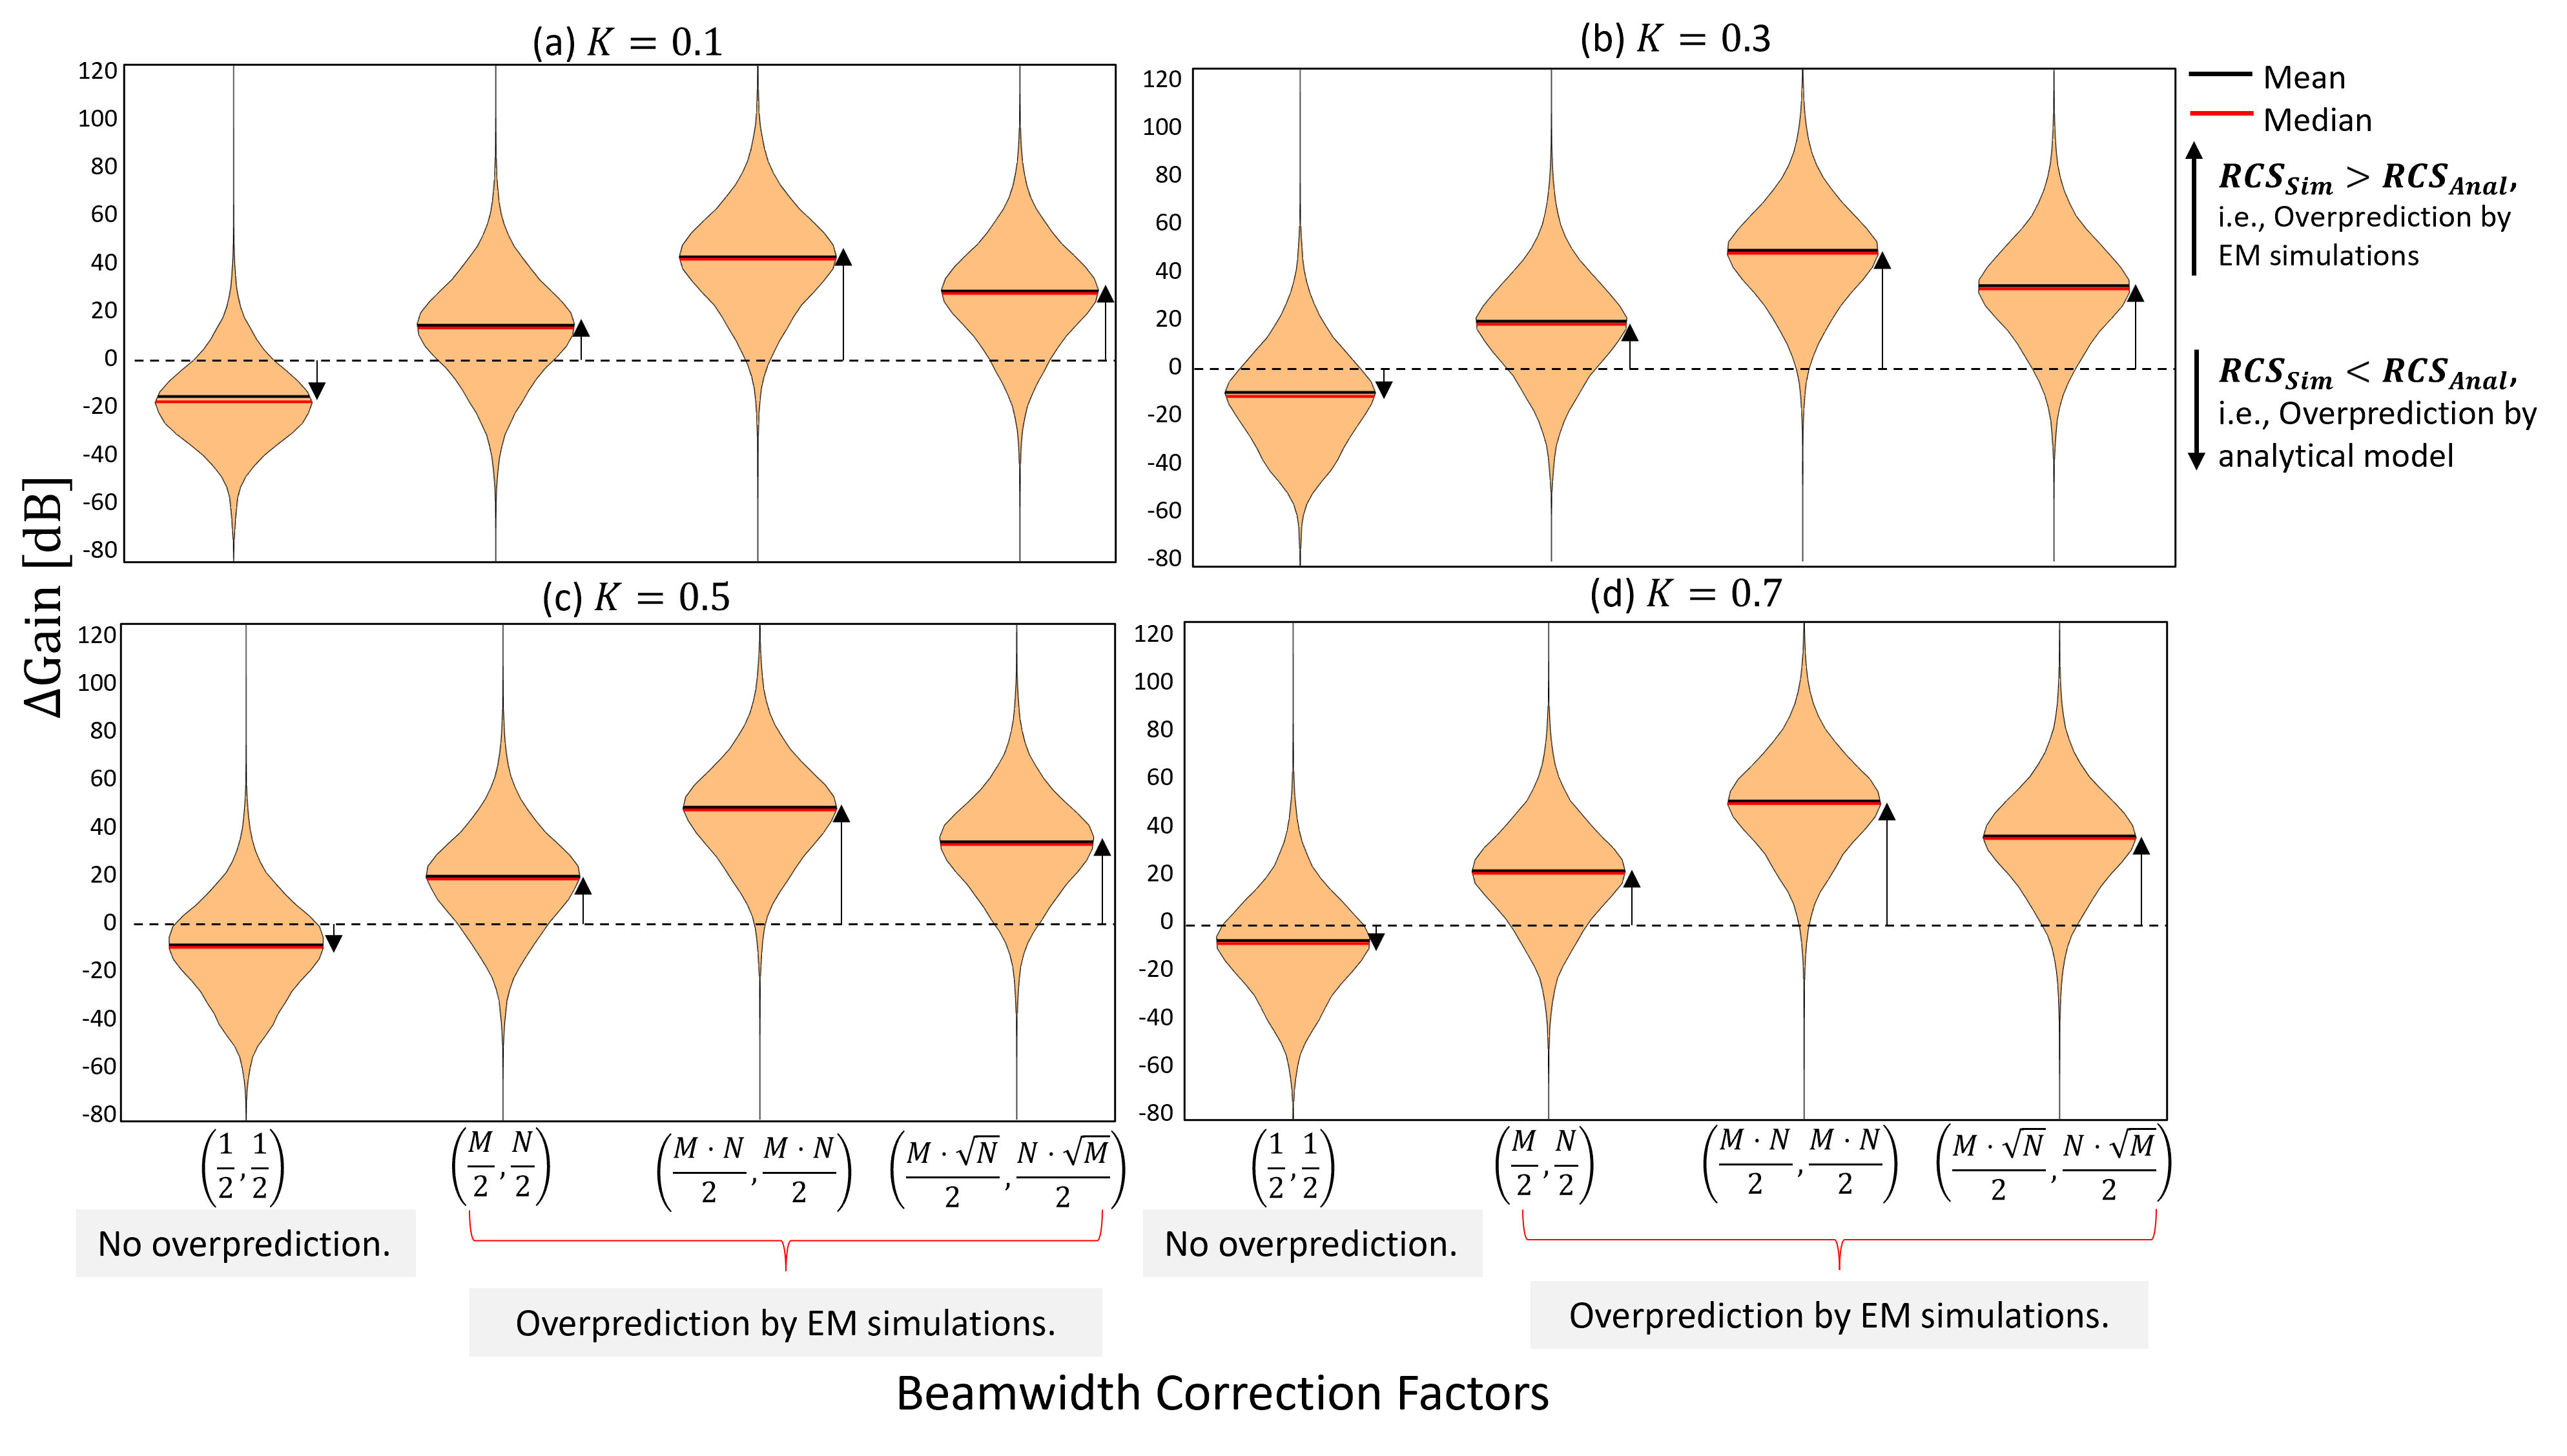
\includegraphics[width=1.0\linewidth]{images/Section 4 Images/Casestudy_orthogonal_BCF}
	\caption{Violin plots illustrating the $\Delta Gain = RCS_{Sim} - RCS_{Anal}.$ in \si{\decibel} for different beamwidth correction factors along the $x$-axis and varying HELIOS size scaling factors $K$ along the four subfigures. Here, $\varphi_{Tx}=\theta_{Tx}=0^\circ$, $\beta_1 =  \dots = \beta_{32}= 0^\circ$, and $\alpha_{1}=...\alpha_{32}=\num{27.6}^\circ$.}
	\label{fig:Casestudy_orthogonal_BCF}
\end{figure}
factors $(\frac{1}{2},\frac{1}{2})$ that are lower than those achieved from simulations, suggesting an overestimation as the mean values in all the four plots are less than zero. Whereas, our analytical model attains mean and median $\Delta Gain>\SI{0}{\decibel}$ values when using beamwidth correction factors of $(\frac{M}{2},\frac{N}{2})$, and $(\frac{M\cdot N}{2},\frac{M\cdot N}{2})$, thus suggesting little overprediction.

Assessing this along increasing $K$, we observe a gradual increase of the mean $\Delta Gain$ values, e.g., for $(\frac{1}{2},\frac{1}{2})$ they are \SI{-18.3}{\decibel}, \SI{-14.6}{\decibel}, \SI{-11.2}{\decibel} and \SI{-7.4}{\decibel}. This shows that overprediction by the analytical model in the case with beamwidth factor $(\frac{1}{2},\frac{1}{2})$ is reduced with increasing HELIOS size. The mean and median values with beamwidth factor $(\frac{M}{2},\frac{N}{2})$ has values $\Delta Gain>\SI{0}{\decibel}$, but less than that of other factors. Thus suggesting this beamwidth factor to be a sensible use for the HELIOS reflector array. 

\textbf{Additional Study: Comparative Results for Varying Reflector Size}

We continue the above case study, however, now $K$ is in range from $[0.1:3]$ \si{\meter} and we change our consideration to the one of a plat plate with $\alpha_{m,n}=\beta_{m,n}=0^\circ$ for all $n \in 1, \dots, 32 = N$ ($m=1$ due to linear array setup). We further explore the urban setting that was previously studied in this extended version, with particular emphasis on factors and assumptions pertaining to reflector properties. The underlying assumptions include an incident wave orthogonal to the reflector base  $\varphi_{Tx}=\theta_{Tx}=0^\circ$ and the prevalent usage of flat plate reflectors i.e., when $\alpha_{m,n}=\beta_{m,n}=0^\circ$. A scaling factor $K$ to determine the reflector size: $a_{m,n} = K \cdot \frac{3}{32}$, and $b_{m,n} = K$, where $K$ $ \forall [0.1:3]$ \si{\meter}. It is important to note that the total dimensions of the \num{32} reflectors preserve the equivalence $a_{m,n}=b_{m,n}$ for all $K$ values.
\begin{figure}[H]
	\centering
	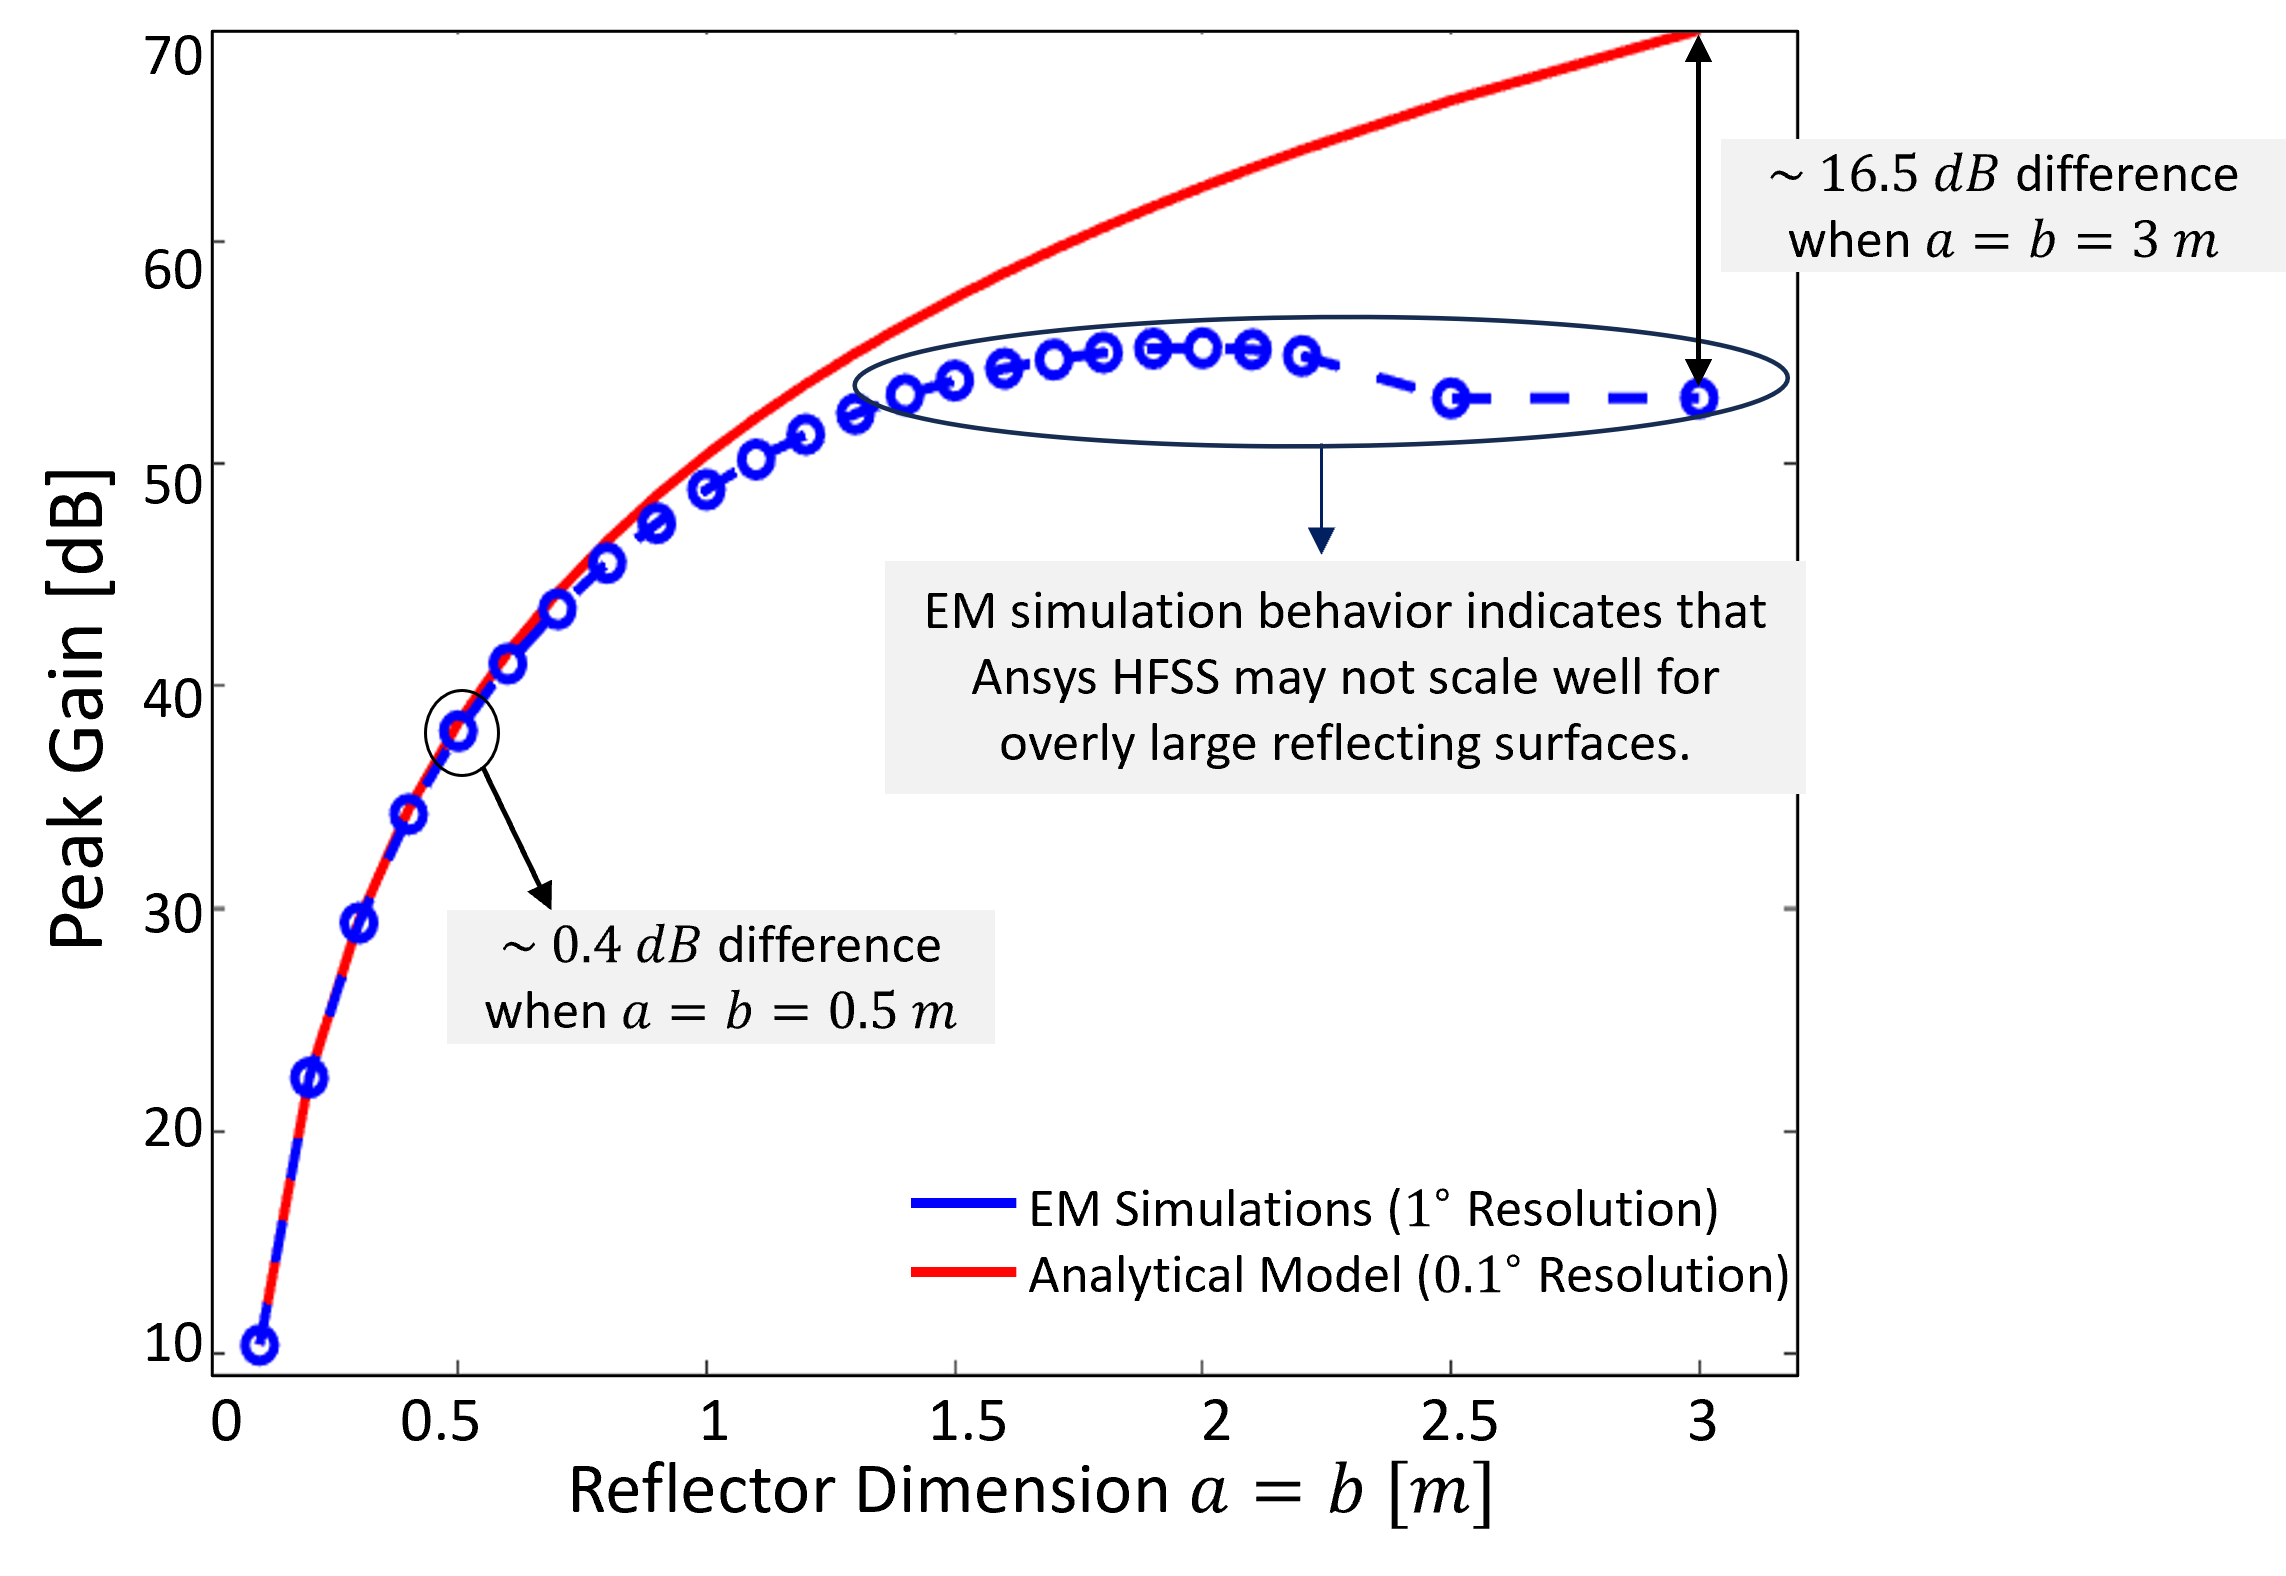
\includegraphics[width=0.8\linewidth]{images/Section 4 Images/casestudy_size}
	\caption{Comparing peak RCS value for $\varphi_{Rx}$, $\theta_{Rx} \in [-90, 90]^\circ$ range between analytical model and EM simulations along different reflecting surface size. Parameters: $\varphi_{Tx}=\theta_{Tx}=0^\circ$, $1 \times 32$ HELIOS with  $\alpha_{m,n}=\beta_{m,n}=0^\circ$ $\forall n \in 1, \dots, N$.}
	\label{fig:casestudy_size}
\end{figure}
\Cref{fig:casestudy_size} shows the peak reflection gain of EM simulations and the analytical model for different reflector sizes. The simulations were carried out with $1^\circ$ angular resolution, whereas our analytical model with $0.1^\circ$, thus, highlighting the speed and accuracy of our model. As expected, on one hand, we wind that the peak gain grows the the reflector side, cf. \Cref{Eq:HELIOS_module}. On the other hand, we observe a breakpoint in this behavior for the simulation-based result curve starting for $a_{m,n}, b_{m,n} > \SI{0.5}{\meter}$, after which the peak gain reduces. But this is not the case with our analytical model, as the model scales with the increasing reflector size directly, see \Cref{Eq:HELIOS_module}. Past this point, the models typically under estimates the rise in peak gain. For the reflector size $a_{m,n}=b_{m,n}=\SI{0.5}{\meter}$, a notable difference of about \SI{0.4}{\decibel} is observed between simulation results and our analytical model, whereas this difference increases to \SI{16.5}{\decibel} for the reflector size $a_{m,n}=b_{m,n}=\SI{3}{\meter}$.

Possible reasons for this discrepancy in the above figure by EM simulations might be reflector mismatches in their properties or a propensity for the simulation to overpredict when using bigger reflectors. It is important to recognize that situations involving huge reflector sizes may not be best handled by this particular Ansys HFSS simulation tool. In conclusion, this extended case study highlights that the findings underscore the need for examination of simulation accuracy, particularly when dealing with larger reflectors, and call for a nuanced understanding of the simulation tool's limitations in certain scenarios.
\subsection{Improved Model Using Inter-module Relations} \label{Improved Model using Inter-module Relations}
Lastly, we improve our analytical model that has been constructed successfully with the beamwidth correction factors of $(\frac{M}{2},\frac{N}{2})$ in the arguments of the respective $\sinc$ functions, cf. \Cref{Eq:HELIOS_module} and \Cref{Eq:HELIOS_array}. In the previous section, we identified that our analytical model does not yet address self-shadowing effects that may occur depending on the HELIOS configuration and the angles of arrival of the incident EM wave. To address this, we consider neighboring HELIOS modules in parts, e.g., there are $N-1$ pairs given $N$ HELIOS modules along the $y$-axis. For each pair, we then assess whether the neighboring module particularly obstruct the incident wave such that the effective reflection area becomes smaller than accounted for so far. This way, we aim to address the overprediction of the RCS peak values against the EM simulation results, as obtained in \Cref{fig:arraymax}.

\begin{figure}[tb]
	\centering
	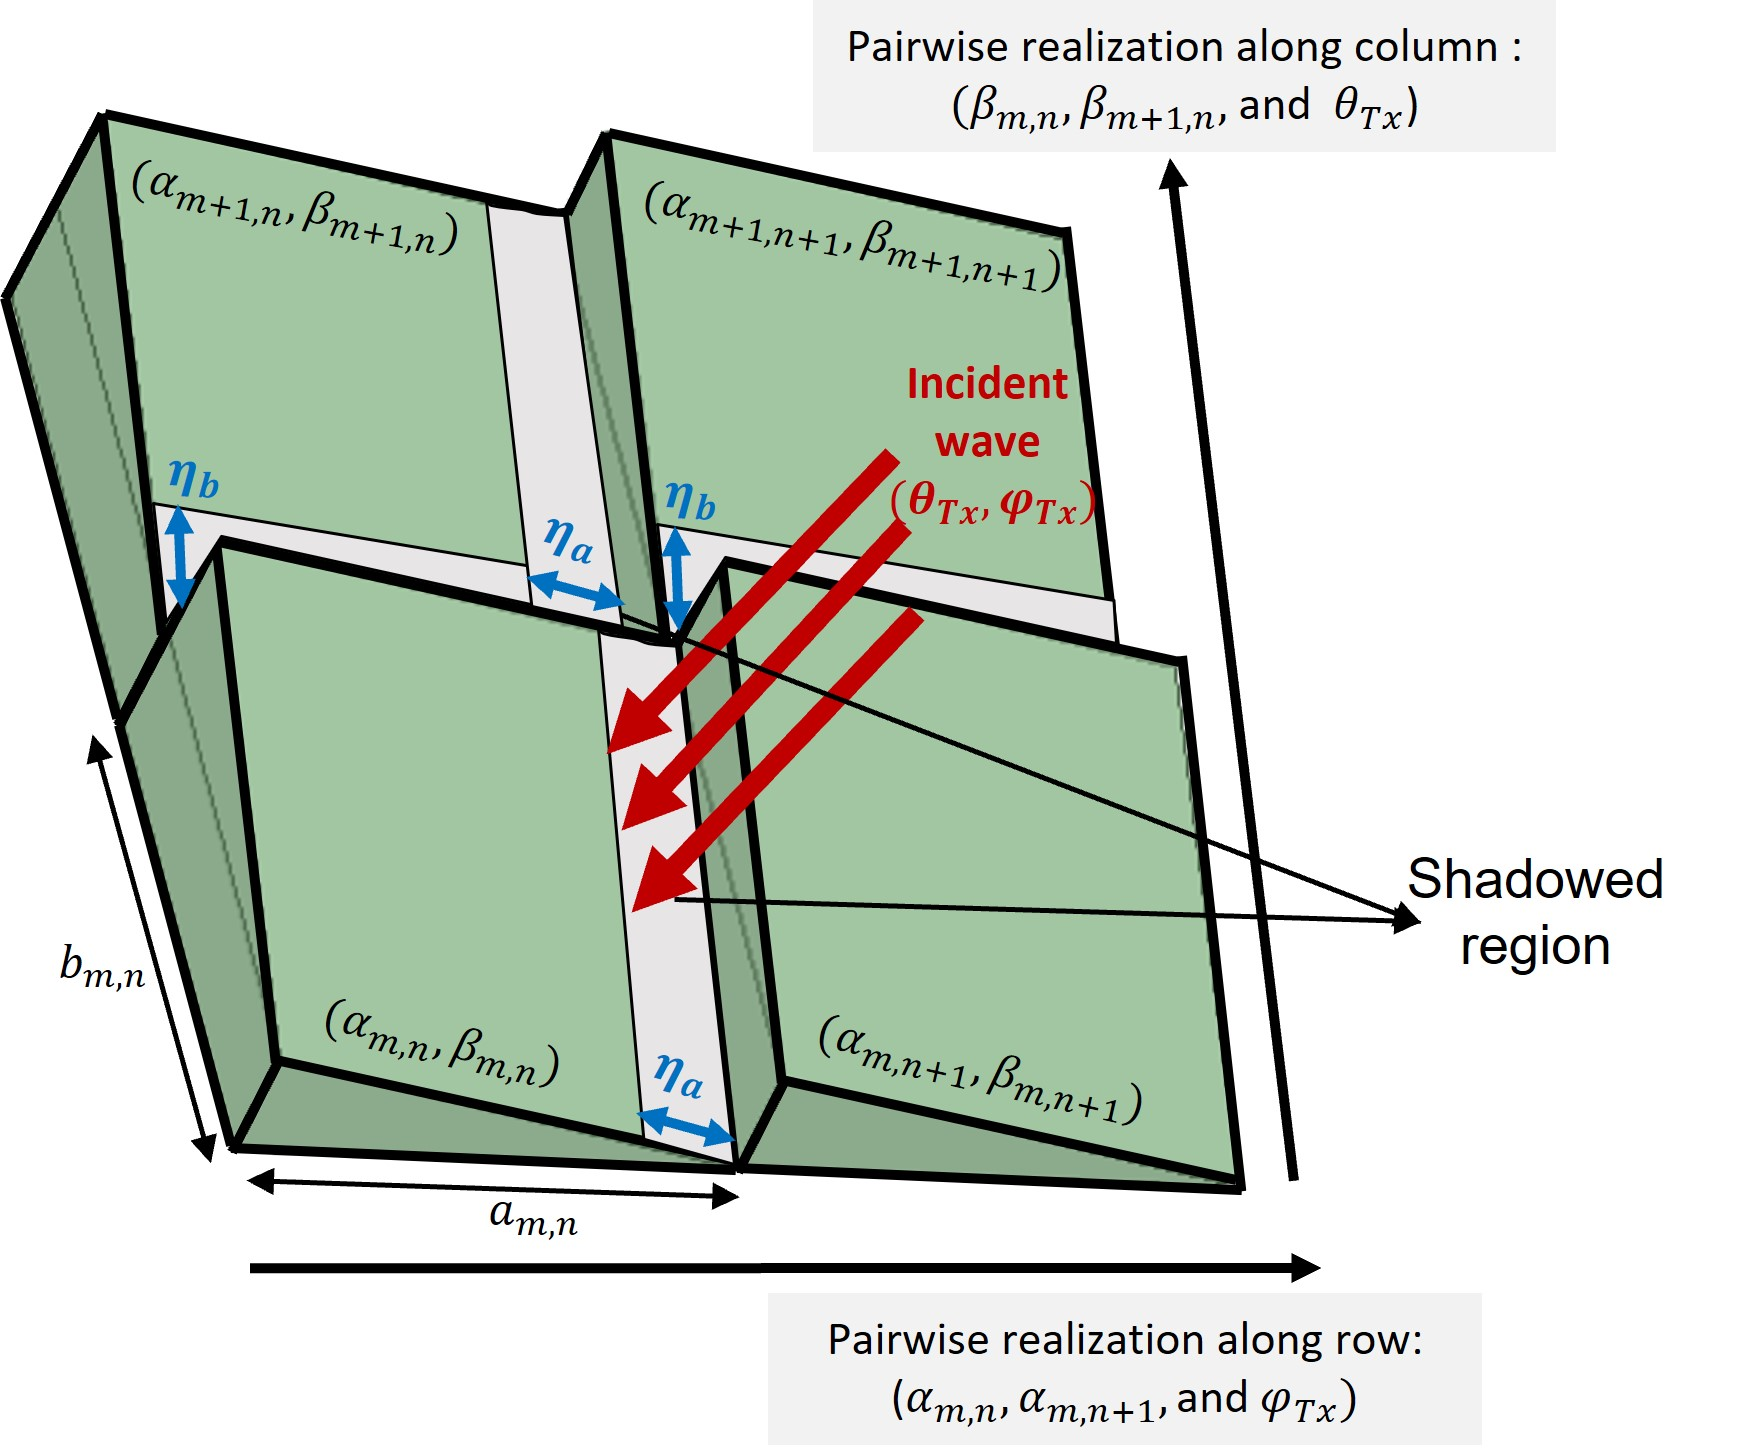
\includegraphics[width=0.65\linewidth]{images/Section 3 Images/ShadowRegion1}
	\caption{Pairwise realization of shadowing region $\eta_{a},\eta_{b}$ along $y$ and $z$ axis for incident wave $(\theta_{Tx}, \varphi_{Tx})$ along the edge for a sample HELIOS array of $2\times 2$ along row and column.}
	\label{fig:Shadow region}
\end{figure}
First, we identify the shadowed fraction of the reflecting surface area along the reflector's edge based on incidence angles $\theta_{Tx}$ and $\varphi_{Tx}$. We split our consideration of this into two parts: one where the angles $\theta_{Tx} > \num{0}^\circ $ and $\varphi_{Tx} > \num{0}^\circ$, and the other where $\theta_{Tx} \leq \num{0}^\circ $ and $\varphi_{Tx} \leq \num{0}^\circ$. We first compute the extent of the shadowed zone along the $y$-axis by taking into account the module pairs' slope angles $\alpha_{m,n}, \alpha_{m,n+1}$, and $\varphi_{Tx}$, as illustrated in \Cref{fig:Shadow region} for a $\num{2}\times \num{2}$ HELIOS reflector array. Likewise, we take into account $\beta_{m,n}, \beta_{m+1,n}$, and $\theta_{Tx}$ to determine the area that is shaded along the $z$-axis. As a result, $\eta_{a}$, and $\eta_{b}$ summarizes the shadowing along the horizontal and vertical edges of module $(m,n)$ from modules $(m,n+1)$ and $(m+1, n)$. For simplicity, we first consider the case of varying $\alpha_{m,n}$ values but with fixed $\beta_{m,n}=\num{0}^\circ$ slopes.

As thus, four separate scenarios arise, as depicted in \Cref{fig:Shadow region1}: In (a) Both the current and neighboring slope angles  values are positive i.e., $\alpha_{m,n}>0^\circ$ and $\alpha_{m,n+1}>0^\circ$. (b) Both the current and neighboring slope angles values are negative i.e., $\alpha_{m,n}<0^\circ$ and $\alpha_{m,n+1}<0^\circ$. (c) The current slope angle $\alpha_{m,n}>0^\circ$, and neighboring slope angles $\alpha_{m,n+1}<0^\circ$. (d) The current slope angle $\alpha_{m,n}<0^\circ$, and neighboring slope angles $\alpha_{m,n+1}>0^\circ$.
\begin{figure}[H]
	\centering
	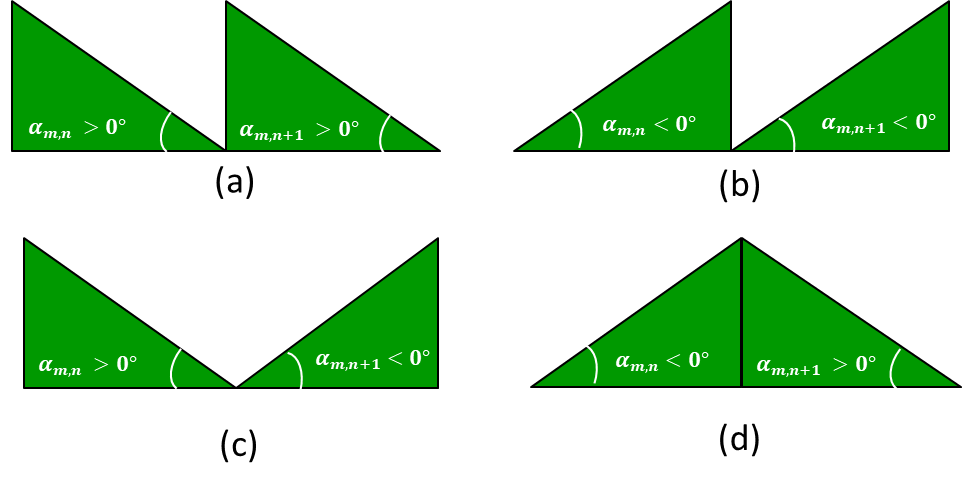
\includegraphics[width=0.85\linewidth]{images/Section 3 Images/ShadowRegion2}
	\caption{Different cases of pairwise realization for simple cases with current and neighboring slope angles $\alpha_{m,n}$, and $\alpha_{m,n+1}$. (a) Both positive slope angles (b) Both negative slope angles (c) Positive-negative slope angles (d) Negative-positive slope angles.}
	\label{fig:Shadow region1}
\end{figure}
This thorough investigation establishes the foundation for deciphering the complex interaction of factors. The calculations of shadowing factors $\eta_{a_{m,n}}$, and $\eta_{b_{m,n}}$ take into account different incident angles cases, i.e., $\theta_{Tx} > \num{0}^\circ $ and $\varphi_{Tx} > \num{0}^\circ$ and also the case when $\theta_{Tx} \leq \num{0}^\circ $ and $\varphi_{Tx} \leq \num{0}^\circ$. To fully comprehend the behavior of the model under various settings, these varied scenarios, see \Cref{fig:Shadow region1} must be included. In particular, because of the way we approached pairwise realization, our tables in \Cref{Table:Shadow region along the row} and \Cref{Table:Shadow region along the column} include formulas for both reflectors, i.e., $\alpha_{m,n}, \alpha_{m,n+1}$ along the row and $\beta_{m,n}, \beta_{m+1,n}$ along the column. \Cref{fig:shadow_derivation} considers the case for the incident angles $\theta_{Tx}=\num{0}^\circ$, and $\varphi_{Tx}>\num{0}^\circ$ and the slope angles $\alpha_{m,n}$, and $\alpha_{m,n+1}$ are positive with $a_{m,n}$ and $a_{m,n+1}$ being the dimension of current and neighboring model. The figure helps in the derivation of the shadowing factor $\eta_{a_{m,n}}$ for this particular case. 

The shadowing factor $\eta_{a_{m,n}}$ from the figure can be derived using the law of sine in the blue shaded triangle. For this particular case, the equation follows as such:
\begin{equation} \label{eq:shadowfactor}
	\frac{\sin(\varphi_{Rx})}{\eta_{a_{m,n}}}=\frac{\sin(90^\circ-\varphi_{Rx}+\alpha_{m,n})}{h_{m,n+1}},
\end{equation}
where $h_{m,n+1}$ is the height of the neighboring reflector given by
\begin{equation}
	h_{m,n+1}= a_{m,n+1} \cdot \tan(\alpha_{m,n+1}).
\end{equation}
The shadowing factor $\eta_{a_{m,n}}$ can be extracted from \Cref{eq:shadowfactor} as
\begin{equation}
	\eta_{a_{m,n}}=h_{m,n+1} \cdot \frac{\sin(\varphi_{Rx})}{\sin(90^\circ-\varphi_{Rx}+\alpha_{m,n})}.
\end{equation}
Similarly, the derivation is considered for different cases in \Cref{fig:Shadow region1} and different incident angles. The derivation of shadow factor $\eta_{b_{m,n}}$ is carried out considering $\theta_{Tx}, \beta_{m,n}, \beta_{m+1,n}, b_{m,n}$, and $b_{m,n+1}$ when $\varphi_{Tx}=0^\circ$. 
\begin{figure}[H]
	\centering
	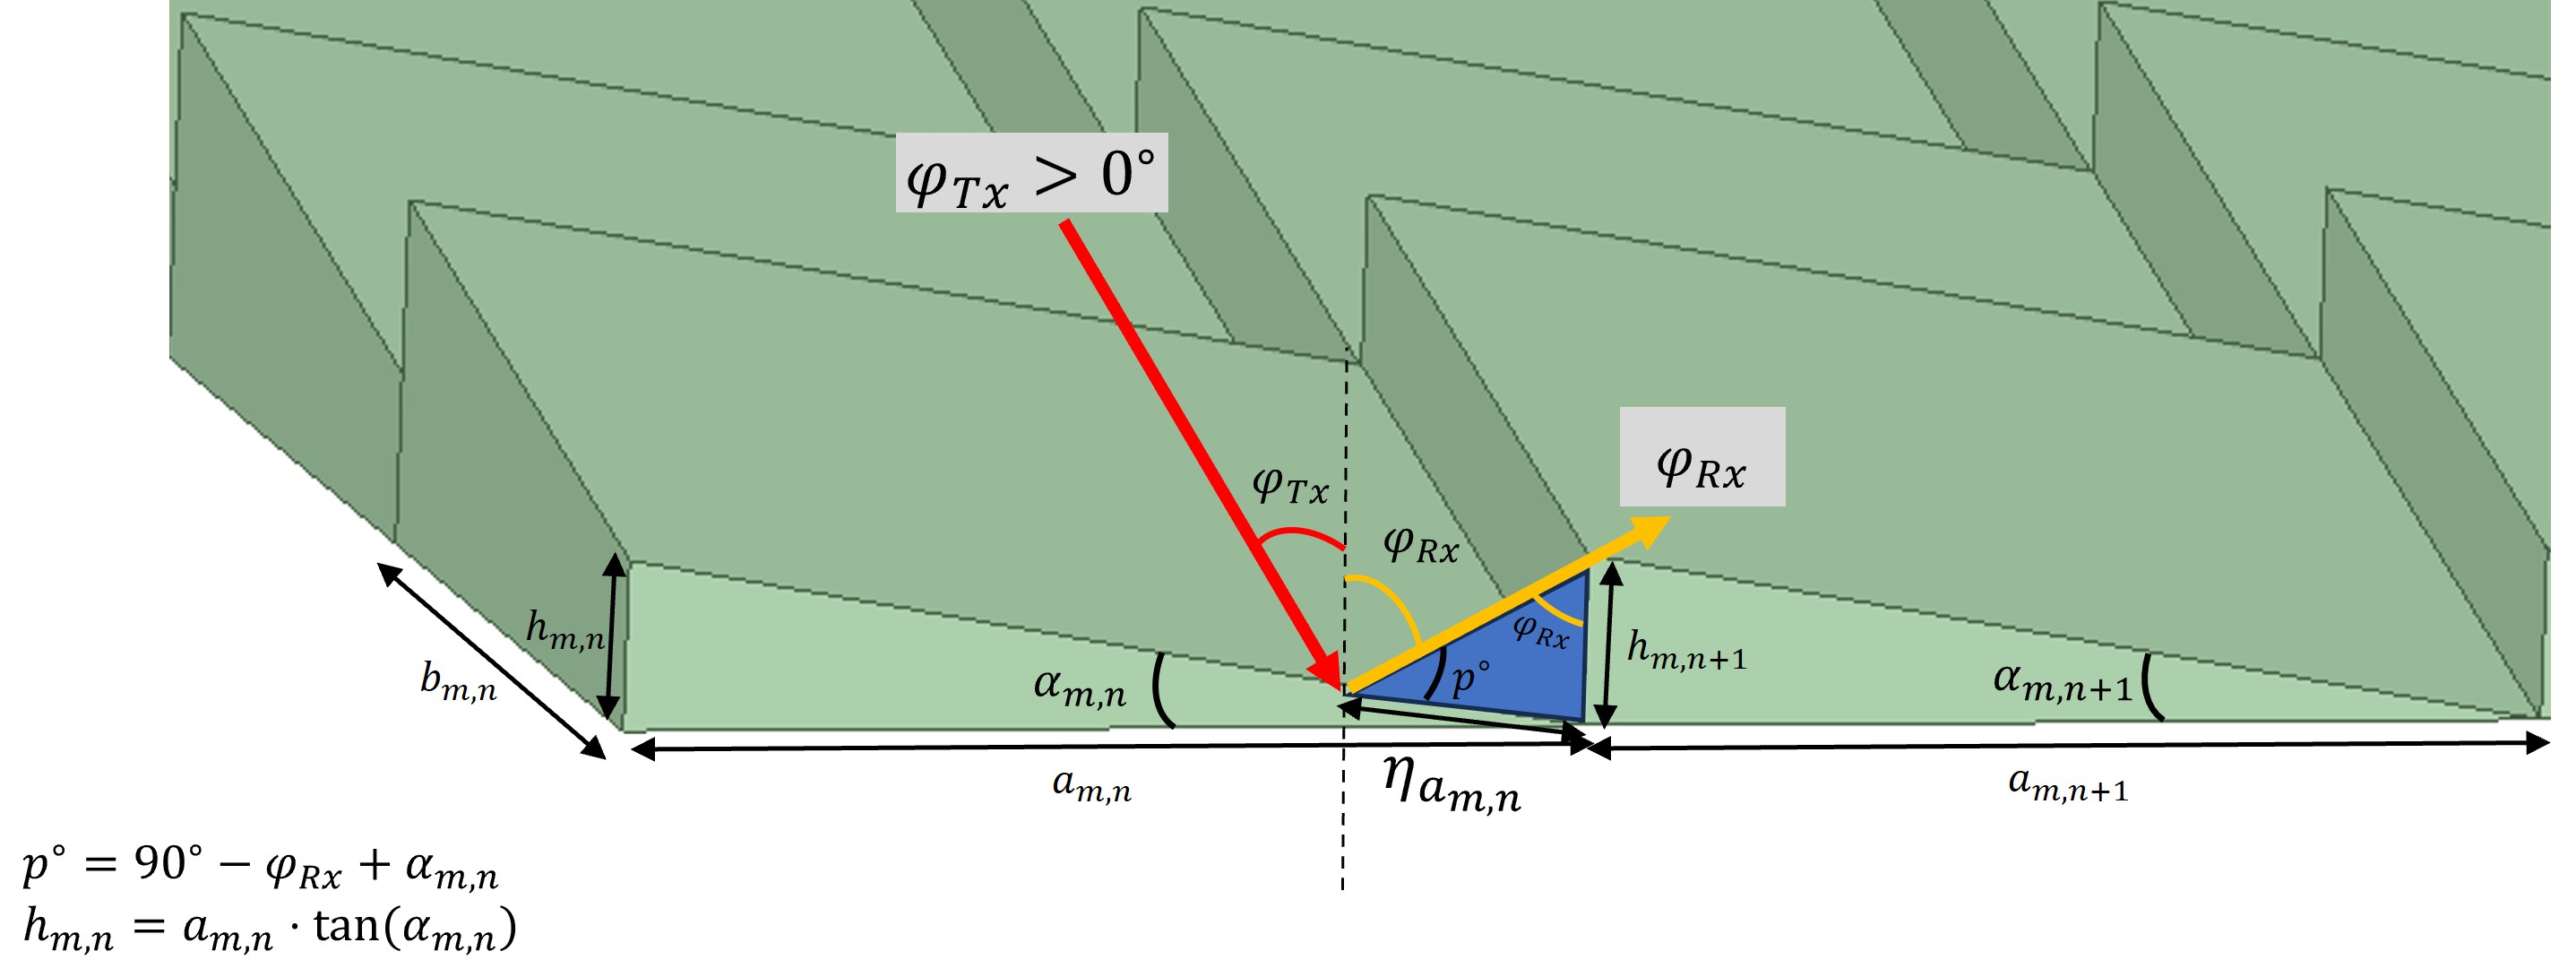
\includegraphics[width=1\linewidth]{images/Section 3 Images/shadow_derivation}
	\caption{Depiction of the shadowing factor $\eta_{a_{m,n}}$ for the case when the incident angles $\theta_{Tx}=\num{0}^\circ$,  $\varphi_{Tx}>\num{0}^\circ$ and the slope angles $\alpha_{m,n}$, and $\alpha_{m,n+1}$ are positive with $a_{m,n}$ and $a_{m,n+1}$. Here, $h_{m,n}$ and $h_{m,n+1}$ are the heights of the current and neighboring reflectors. }
	\label{fig:shadow_derivation}
\end{figure}
Using the shadowing factors $\eta_{a_{m,n}}$, and $\eta_{b_{m,n}}$ for the current and neighboring reflector with $m$ and $n$ indices, the \Cref{Table:Shadow region along the row} and \Cref{Table:Shadow region along the column} provides a detailed presentation of the obtained derived formulas for the shadowed region along the rows and columns, respectively.

We determine the effective reflecting surface size $a_{m,n}^* \times b_{m,n}^*$ as shown in \Cref{Eq:effective region_a} and \Cref{Eq:effective region_b}.
\begin{equation} \label{Eq:effective region_a}
	a_{m,n}^*= (1-\eta_{a_{m,n}})\cdot a_{m,n}
\end{equation}
\begin{equation} \label{Eq:effective region_b}
	b_{m,n}^*= (1-\eta_{b_{m,n}})\cdot b_{m,n}
\end{equation}
 Here, $\eta_{a_{m,n}}$ is for pairwise realization of model along the row, whereas $\eta_{b_{m,n}}$ is along the column.
 
\begin{table}[H] % H -> dieses objekt wird genau da wo der code steht festgenagelt
	\footnotesize
	\caption{Shadowed region for the first reflector along the row and column for cases in \Cref{fig:Shadow region1}. }
	\label{Table:Shadow region along the row}
	\centering
	\begin{tabular}{c|c|c}
	\textbf{Slope Angle} & \textbf{Incident} & \textbf{Shadowing Factor Formulae at the First Reflector}\\
	\hline
	\multirow{2}{*}{\begin{tabular}{@{}c@{}c@{}c@{}}$\alpha_{m,n}>0^\circ $\\ $\alpha_{m,n+1}>0^\circ $ \\ $\beta_{m,n}>0^\circ $\\ $\beta_{m+1,n}>0^\circ $ \end{tabular}}
	& 
	\begin{tabular}{@{}c@{}} $\varphi_{Tx}>0^\circ $ \\ $\theta_{Tx}>0^\circ $ \end{tabular}
	&
	\begin{math} \label{eq:1:SR}
		\begin{aligned}
			\eta_{a_{m,n}} &= \frac{a_{m,n+1}}{a_{m,n}} \cdot \tan(\alpha_{m,n+1}) \cdot \frac{\sin(\varphi_{Tx})}{\cos(-\varphi_{Tx}+ \alpha_{m,n})}, \varphi_{Tx}>0^\circ \\
			\eta_{b_{m,n}} &= 0, \theta_{Tx} >0^\circ \\
		\end{aligned}		
	\end{math}\\
	\cline{2-3}
	& 
	\begin{tabular}{@{}c@{}}$\varphi_{Tx} \leq 0^\circ $ \\ $\theta_{Tx} \leq 0^\circ $ \end{tabular}
	&
	\begin{math}\label{eq:2:SR}
		\begin{aligned}
			\eta_{a_{m,n}} &=
			\begin{cases}
				\frac{a_{m,n+1}}{a_{m,n}} \cdot \tan(\alpha_{m,n+1}) \cdot \frac{\sin(-\varphi_{Tx}+ 2\cdot \alpha_{m,n+1})}{\cos(-\varphi_{Tx}+ \alpha_{m,n}-2 \cdot \alpha_{m,n+1})}, &  \varphi_{Tx} > -90^\circ + \alpha_{m,n} \\
				1, & \varphi_{Tx} < -90^\circ + \alpha_{m,n} \\
			\end{cases}\\
			\eta_{b_{m,n}} &=
			\begin{cases}
				0, & \theta_{Tx} >-90^\circ + \beta_{m+1,n}\\
				1, & \theta_{Tx} < -90^\circ + \beta_{m+1,n}\\
			\end{cases}
		\end{aligned}		
	\end{math}\\
	\hline
	\multirow{2}{*}{\begin{tabular}{@{}c@{}c@{}c@{}}$\alpha_{m,n}<0^\circ $\\ $\alpha_{m,n+1}<0^\circ $ \\ $\beta_{m,n}<0^\circ $\\ $\beta_{m+1,n}<0^\circ $ \end{tabular}}
	& 
	\begin{tabular}{@{}c@{}}$\varphi_{Tx}>0^\circ $ \\ $\theta_{Tx}>0^\circ $ \end{tabular}
	&
	\begin{math}
		\begin{aligned}
			\eta_{a_{m,n}} &=
			\begin{cases}
				0, & \varphi_{Tx} < 90^\circ + \alpha_{m,n}\\
				1, & \varphi_{Tx} > 90^\circ + \alpha_{m,n}\\
			\end{cases}\\
			\eta_{b_{m,n}} &=
			\begin{cases}
				\frac{b_{m+1,n}}{b_{m,n}} \cdot \tan(\beta_{m+1,n}) \cdot \frac{\sin(-\theta_{Tx}+2 \cdot \beta_{m,n})}{\cos(-\theta_{Tx}-2 \cdot \beta_{m,n}+ \beta_{m+1,n})}, &  \theta_{Tx} < 90^\circ + \beta_{m,n} \\
				1, & \theta_{Tx} > 90^\circ + \beta_{m,n} \\
			\end{cases}\\
		\end{aligned}		
	\end{math}\\
	\cline{2-3}
	& 
	\begin{tabular}{@{}c@{}}$\varphi_{Tx} \leq 0^\circ $ \\ $\theta_{Tx} \leq 0^\circ $ \end{tabular}
	&
	\begin{math}
		\begin{aligned}
			\eta_{a_{m,n}} &= 0, \varphi_{Tx} < 0^\circ \\
			\eta_{b_{m,n}} &= \frac{b_{m+1,n}}{b_{m,n}} \cdot \tan(\beta_{m+1,n}) \cdot \frac{\sin(\theta_{Tx})}{\cos(-\theta_{Tx}+ \beta_{m,n})}, \theta_{Tx} < 0^\circ \\
		\end{aligned}		
	\end{math}\\
	\hline
	\multirow{2}{*}{\begin{tabular}{@{}c@{}c@{}c@{}}$\alpha_{m,n}>0^\circ $\\ $\alpha_{m,n+1}<0^\circ $ \\ $\beta_{m,n}>0^\circ $\\ $\beta_{m+1,n}<0^\circ $ \end{tabular}}
	& 
	\begin{tabular}{@{}c@{}}$\varphi_{Tx}>0^\circ $ \\ $\theta_{Tx}>0^\circ $ \end{tabular}
	&
	\begin{math}
		\begin{aligned}
			\eta_{a_{m,n}} &=
			\begin{cases}
				0, & \varphi_{Tx} < 90^\circ + \alpha_{m,n+1}\\
				\frac{a_{m,n+1}}{a_{m,n}}\sqrt{1+ \tan^2 (\alpha_{m,n+1})} \frac{\sin(\varphi_{Tx}+ \alpha_{m,n+1}- 90^\circ)}{\cos(-\varphi_{Tx}+ \alpha_{m,n})}, &\varphi_{Tx} > 90^\circ + \alpha_{m,n+1}\\
			\end{cases}\\
			\eta_{b_{m,n}} &=
			\begin{cases}
				0, & \theta_{Tx} < 90^\circ + \beta_{m,n}\\
				1, & \theta_{Tx} > 90^\circ + \beta_{m,n}\\
			\end{cases}\\
		\end{aligned}		
	\end{math}\\
	\cline{2-3}
	& 
	\begin{tabular}{@{}c@{}}$\varphi_{Tx} \leq 0^\circ $ \\ $\theta_{Tx} \leq 0^\circ $ \end{tabular}
	&
	\begin{math}
		\begin{aligned}
			\eta_{a_{m,n}} &=
			\begin{cases}
				0, & \varphi_{Tx} > -90^\circ + \alpha_{m,n}\\
				1, & \varphi_{Tx} < -90^\circ + \alpha_{m,n}\\
			\end{cases}\\
			\eta_{b_{m,n}} &=
			\begin{cases}
				0, & \theta_{Tx} > -90^\circ + \beta_{m+1,n}\\
				\frac{b_{m+1,n}}{b_{m,n}}\sqrt{1+ \tan^2 (\beta_{m+1,n})} \frac{\sin(\theta_{Tx}+ \beta_{m+1,n}- 90^\circ)}{\cos(-\theta_{Tx}+ \beta_{m,n})}, & \theta_{Tx} < -90^\circ + \beta_{m+1,n}\\
			\end{cases}\\
		\end{aligned}		
	\end{math}\\
	\hline
	\multirow{2}{*}{\begin{tabular}{@{}c@{}c@{}c@{}}$\alpha_{m,n}<0^\circ $\\ $\alpha_{m,n+1}>0^\circ $ \\ $\beta_{m,n} <0^\circ $\\ $\beta_{m+1,n}>0^\circ $ \end{tabular}}
	& 
	\begin{tabular}{@{}c@{}}$\varphi_{Tx}>0^\circ $ \\ $\theta_{Tx}>0^\circ $ \end{tabular}
	&
	\begin{math}
		\begin{aligned}
			\eta_{a_{m,n}} &=
			\begin{cases}
				0, & \varphi_{Tx} < 90^\circ - \alpha_{m,n+1}\\
				1, & \varphi_{Tx} > 90^\circ - \alpha_{m,n+1}\\
			\end{cases}\\
			\eta_{b_{m,n}} &= 0, \theta_{Tx} > 0^\circ\\
		\end{aligned}		
	\end{math}\\
	\cline{2-3}
	& 
	\begin{tabular}{@{}c@{}}$\varphi_{Tx} \leq 0^\circ $ \\ $\theta_{Tx} \leq 0^\circ $ \end{tabular}
	&
	\begin{math}
		\begin{aligned}
			\eta_{a_{m,n}} &= 0,   \varphi_{Tx} > 0^\circ\\
			\eta_{b_{m,n}} &=
			\begin{cases}
				0, & \theta_{Tx} > -90^\circ + \beta_{m+1,n}\\
				1, & \theta_{Tx} < -90^\circ + \beta_{m+1,n}\\
			\end{cases}
		\end{aligned}		
	\end{math}
	\end{tabular}
\end{table}
\begin{table}[tb] % H -> dieses objekt wird genau da wo der code steht festgenagelt
		\footnotesize
	\caption{Shadowed region for the second reflector along the row and column for cases in \Cref{fig:Shadow region1}.}
	\label{Table:Shadow region along the column}
	\centering
	\begin{tabular}{c|c|c}
		\textbf{Slope Angle} & \textbf{Incident} & \textbf{Shadowing Factor Formulae at the Second Reflector}\\
		\hline
		\multirow{2}{*}{\begin{tabular}{@{}c@{}c@{}c@{}}$\alpha_{m,n}>0^\circ $\\ $\alpha_{m,n+1}>0^\circ $ \\ $\beta_{m,n}>0^\circ $\\ $\beta_{m+1,n}>0^\circ $ \end{tabular}}
		& 
		\begin{tabular}{@{}c@{}}$\varphi_{Tx}>0^\circ $ \\ $\theta_{Tx}>0^\circ $ \end{tabular}
		&
		\begin{math}
			\begin{aligned}
				\eta_{a_{m,n+1}} &= 0, \varphi_{Tx} >0^\circ \\
				\eta_{b_{m+1,n}} &= \frac{b_{m,n}}{b_{m+1,n}} \cdot \tan(\beta_{m,n}) \cdot \frac{\sin(\theta_{Tx})}{\cos(-\theta_{Tx}+ \beta_{m+1,n})}, \theta_{Tx}>0^\circ \\
			\end{aligned}		
		\end{math}\\ 
		\cline{2-3}
		& 
		\begin{tabular}{@{}c@{}}$\varphi_{Tx} \leq 0^\circ $ \\ $\theta_{Tx} \leq 0^\circ $ \end{tabular}
		&
	\begin{math}
		\begin{aligned}
			\eta_{a_{m,n+1}} &=
			\begin{cases}
				\frac{a_{m,n}}{a_{m,n+1}} \cdot \tan(\alpha_{m,n}) \cdot \frac{\sin(-\varphi_{Tx}+2 \cdot \alpha_{m,n})}{\cos(-\varphi_{Tx} -2 \cdot \alpha_{m,n} + \alpha_{m,n+1})}, &  \varphi_{Tx} < 90^\circ + \alpha_{m,n} \\
				1, & \varphi_{Tx} > 90^\circ + \alpha_{m,n} \\
			\end{cases}\\
			\eta_{b_{m+1,n}} &=
			\begin{cases}
				0, & \theta_{Tx} < 90^\circ + \beta_{m+1,n}\\
				1, & \theta_{Tx} > 90^\circ + \beta_{m+1,n}\\
			\end{cases}\\
		\end{aligned}		
	\end{math}\\
		\hline
		\multirow{2}{*}{\begin{tabular}{@{}c@{}c@{}c@{}}$\alpha_{m,n}<0^\circ $\\ $\alpha_{m,n+1}<0^\circ $ \\ $\beta_{m,n}<0^\circ $\\ $\beta_{m+1,n}<0^\circ $ \end{tabular}}
		& 
		\begin{tabular}{@{}c@{}}$\varphi_{Tx}>0^\circ $ \\ $\theta_{Tx}>0^\circ $ \end{tabular}
		&
		\begin{math}
			\begin{aligned}
				\eta_{a_{m,n+1}} &= \frac{a_{m,n}}{a_{m,n+1}} \cdot \tan(\alpha_{m,n}) \cdot \frac{\sin(\varphi_{Tx})}{\cos(-\varphi_{Tx}+ \alpha_{m,n+1})}, \varphi_{Tx} < 0^\circ \\
				\eta_{b_{m+1,n}} &= 0,\theta_{Tx} < 0^\circ \\
			\end{aligned}		
		\end{math}\\ 
		\cline{2-3}
		& 
		\begin{tabular}{@{}c@{}}$\varphi_{Tx} \leq 0^\circ $ \\ $\theta_{Tx} \leq 0^\circ $ \end{tabular}
		&
			\begin{math}
			\begin{aligned}
				\eta_{a_{m,n+1}} &=
				\begin{cases}
					0, & \varphi_{Tx} < 90^\circ + \alpha_{m,n+1}\\
					1, & \varphi_{Tx} > 90^\circ + \alpha_{m,n+1}\\
				\end{cases}\\
				\eta_{b_{m+1,n}} &=
				\begin{cases}
					0, & \theta_{Tx} < 90^\circ + \beta_{m,n}\\
					\frac{b_{m,n}}{b_{m+1,n}} \cdot \sqrt{1+ \tan^2 (\beta_{m,n})} \cdot \frac{\sin(\theta_{Tx}+ \beta_{m,n}- 90^\circ)}{\cos(-\theta_{Tx}+ \beta_{m+1,n})}, & \theta_{Tx} > 90^\circ + \beta_{m,n}\\
				\end{cases}
			\end{aligned}		
		\end{math}\\
		\hline
		\multirow{2}{*}{\begin{tabular}{@{}c@{}c@{}c@{}}$\alpha_{m,n}>0^\circ $\\ $\alpha_{m,n+1}<0^\circ $ \\ $\beta_{m,n}>0^\circ $\\ $\beta_{m+1,n}<0^\circ $ \end{tabular}}
		& 
		\begin{tabular}{@{}c@{}}$\varphi_{Tx}>0^\circ $ \\ $\theta_{Tx}>0^\circ $ \end{tabular}
		&
	\begin{math}
		\begin{aligned}
			\eta_{a_{m,n+1}} &=
			\begin{cases}
				0, & \varphi_{Tx} >-90^\circ + \alpha_{m,n}\\
				1, & \varphi_{Tx} < -90^\circ + \alpha_{m,n}\\
			\end{cases}\\
			\eta_{b_{m+1,n}} &=
			\begin{cases}
				\frac{b_{m,n}}{b_{m+1,n}} \cdot \tan(\beta_{m,n}) \cdot \frac{\sin(-\theta_{Tx}+ 2\cdot \beta_{m,n})}{\cos(-\theta_{Tx}+ \beta_{m,n}-2 \cdot \beta_{m+1,n})}, &  \theta_{Tx} > -90^\circ + \beta_{m+1,n} \\
				1, & \theta_{Tx} < -90^\circ + \beta_{m+1,n} \\
			\end{cases}\\
		\end{aligned}		
	\end{math}\\
		\cline{2-3}
		& 
		\begin{tabular}{@{}c@{}}$\varphi_{Tx} \leq 0^\circ $ \\ $\theta_{Tx} \leq 0^\circ $ \end{tabular}
		&
		\begin{math}
			\begin{aligned}
				\eta_{a_{m,n+1}} &=
				\begin{cases}
					0, & \varphi_{Tx} > -90^\circ + \alpha_{m,n}\\
					\frac{a_{m,n}}{a_{m,n+1}} \cdot \sqrt{1+ \tan^2 (\alpha_{m,n})} \cdot \frac{\sin(\varphi_{Tx}+ \alpha_{m,n}- 90^\circ)}{\cos(-\varphi_{Tx}+ \alpha_{m,n+1})}, & \varphi_{Tx} < -90^\circ + \alpha_{m,n}\\
				\end{cases}\\
				\eta_{b_{m+1,n}} &=
				\begin{cases}
					0, & \theta_{Tx} > -90^\circ + \beta_{m+1,n}\\
					1, & \theta_{Tx} < -90^\circ + \beta_{m+1,n}\\
				\end{cases} \\
			\end{aligned}	
		\end{math}\\
		\hline
		\multirow{2}{*}{\begin{tabular}{@{}c@{}c@{}c@{}}$\alpha_{m,n}<0^\circ $\\ $\alpha_{m,n+1}>0^\circ $ \\ $\beta_{m,n} <0^\circ $\\ $\beta_{m+1,n}>0^\circ $ \end{tabular}}
		& 
		\begin{tabular}{@{}c@{}}$\varphi_{Tx}>0^\circ $ \\ $\theta_{Tx}>0^\circ $ \end{tabular}
		&
		\begin{math}
			\begin{aligned}
				\eta_{a_{m,n+1}} &= 0, \varphi_{Tx} > 0^\circ\\
				\eta_{b_{m+1,n}} &=
				\begin{cases}
					0, & \theta_{Tx} < 90^\circ - \beta_{m,n}\\
					1, & \theta_{Tx} > 90^\circ - \beta_{m,n}\\
				\end{cases}\\
			\end{aligned}		
		\end{math}\\
		\cline{2-3}
		& 
		\begin{tabular}{@{}c@{}}$\varphi_{Tx} \leq 0^\circ $ \\ $\theta_{Tx} \leq 0^\circ $ \end{tabular}
		&
		\begin{math}
			\begin{aligned}
				\eta_{a_{m,n+1}} &=
				\begin{cases}
					0, & \varphi_{Tx} > -90^\circ + \alpha_{m,n+1}\\
					1, & \varphi_{Tx} < -90^\circ + \alpha_{m,n+1}\\
				\end{cases}\\
				\eta_{b_{m+1,n}} &= 0, \theta_{Tx} > 0^\circ\\
			\end{aligned}		
		\end{math}	\\
	\end{tabular}
\end{table}
Our new methodology reveals an improved analytical model that exemplifies a clear dependency as described in  \Cref{Eq:RCS_SUMMATION_SR}.
\begin{equation}\label{Eq:RCS_SUMMATION_SR}
	\sigma_{Array}= \left(\sum_{n=1}^{N}\sum_{m=1}^{M} \sqrt{\sigma_{module} \left( a_{m,n}^*, b_{m,n}^*, \alpha_{m,n}, \beta_{m,n} \right) } \right)^2
\end{equation}
To further explore the nuances of these scenarios, \Cref{fig:Shadow region2} depicts the shadowed region behavior of the two reflectors for incident azimuth angles $\varphi_{Tx} \in [-90:90]^\circ$ for the first case with positive slope angles of current and neighboring reflectors i.e., $\alpha_{m,n}=\alpha_{m,n+1}=\num{10}^\circ$, where $a_{m,n}=b_{m,n}=\SI{10}{\centi\meter}$, while $\beta_{m,n}=0^\circ$, and $\theta_{Tx}=0^\circ$, see \Cref{fig:Shadow region1}. 

\begin{figure}[tb]
	\centering
	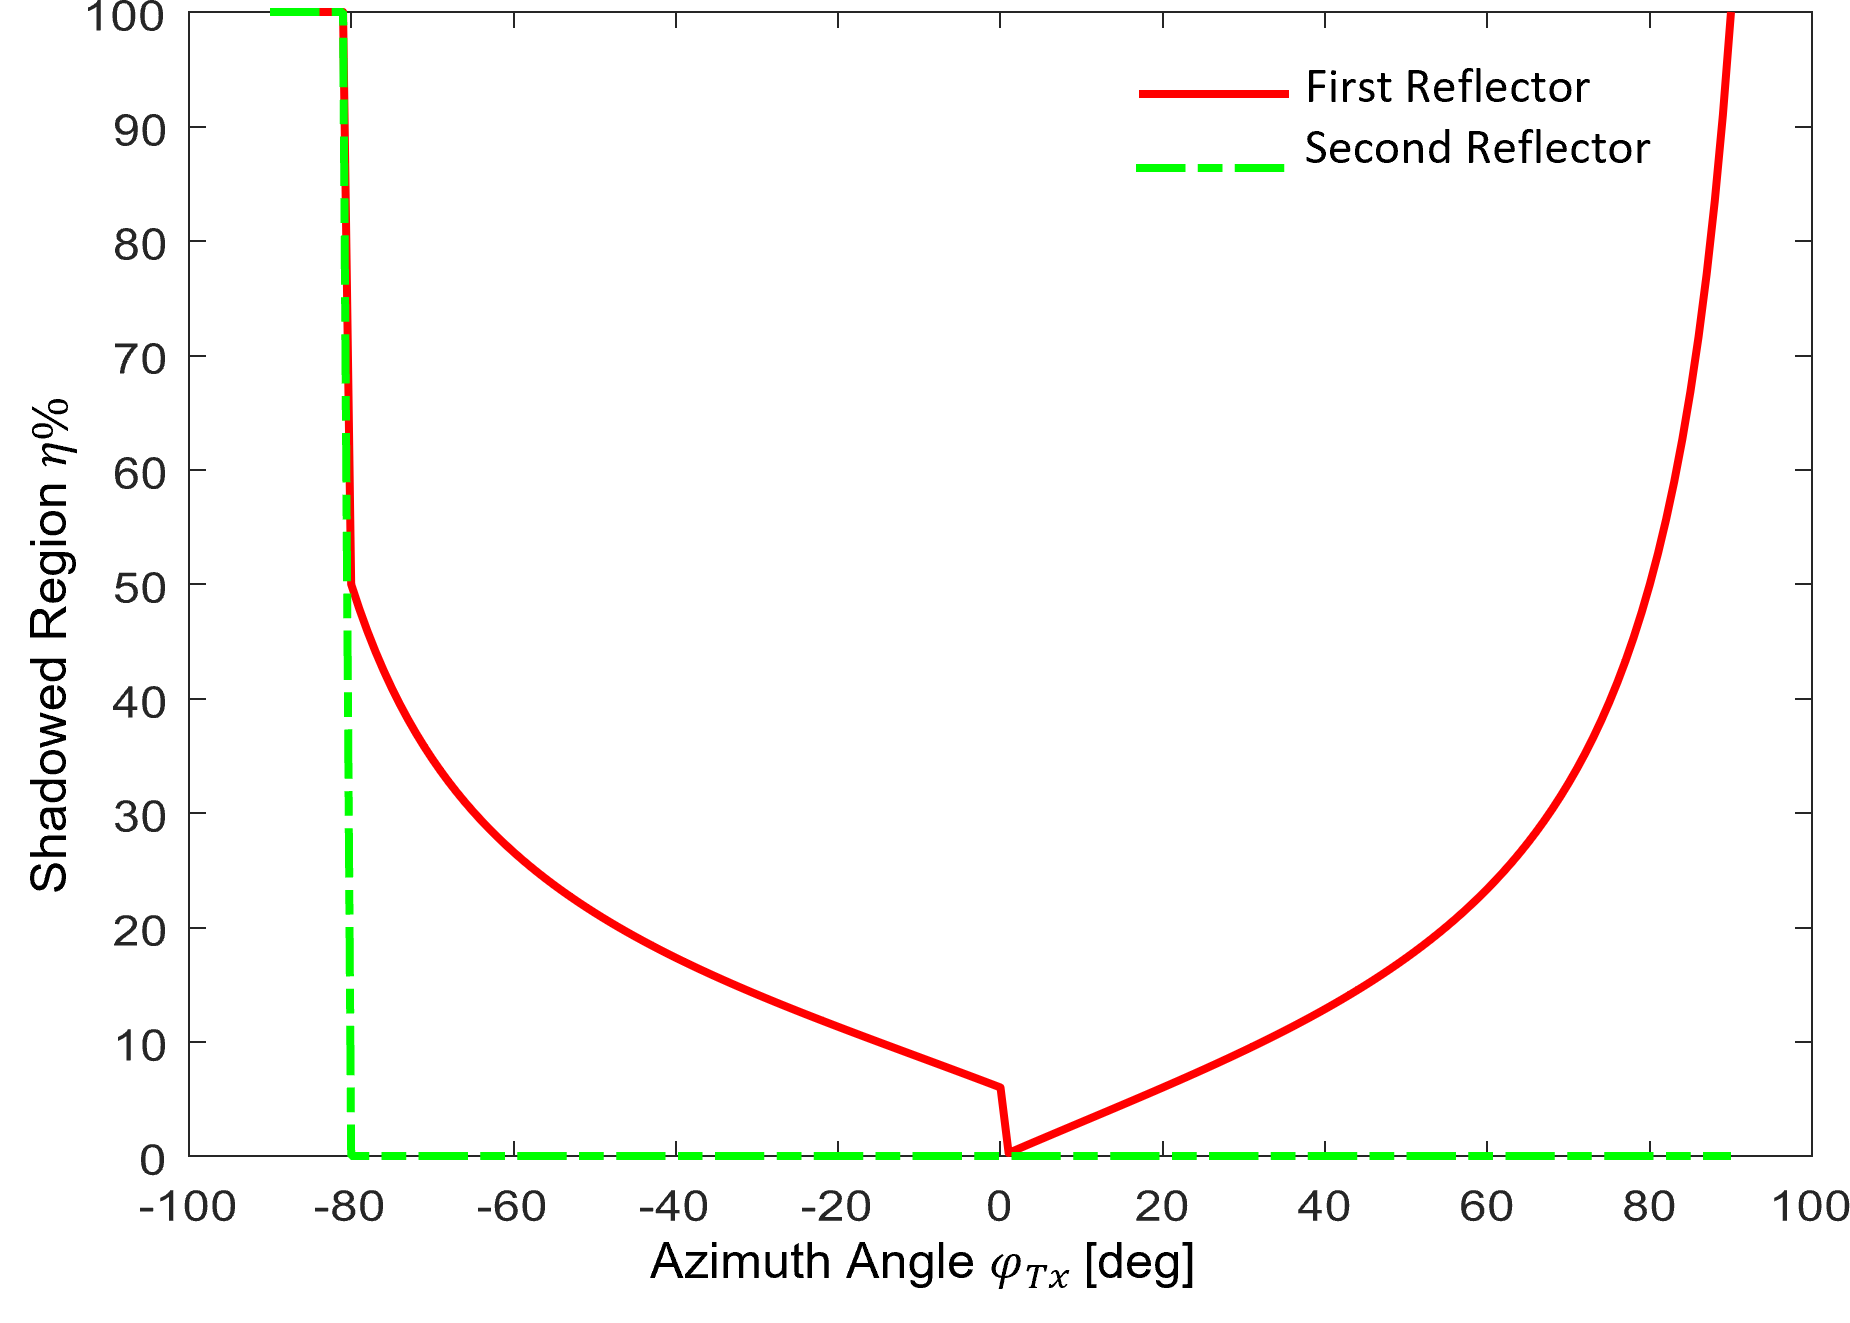
\includegraphics[width=0.7\linewidth]{images/Section 3 Images/ShadowRegion3}
	\caption{Plot depicting the amount of region shadowed for different incident azimuth angles $\varphi_{Tx} \in [-90:90]^\circ$ for simple case with  $\alpha_{m,n}=\alpha_{m,n+1}=\num{10}^\circ$ and $a_{m,n}=b_{m,n}=\SI{10}{\centi\meter}$ while $\beta_{m,n}=0^\circ$, and $\theta_{Tx}=0^\circ$. }
	\label{fig:Shadow region2}
\end{figure}
When one looks at the peak gain plot in \Cref{fig:arraymax_SR}, the transformational impact of this integration is evident when compared to the peak gain plot in \Cref{fig:arraymax}. After applying our modified model with the consideration of shadowed region $\eta_{a_{m,n}}$ and $\eta_{b_{m,n}}$, we achieved a significant improvement in the difference in peak gain between analytical and simulation models.

A noticeable difference of \SI{0.02}{\decibel} is observed between analytical model and EM simulation results at $\num{1}\times \num{8}$ HELIOS reflector array when compared to the results in \Cref{fig:arraymax} with \SI{0.4}{\decibel}. In similar manner, the difference of about \SI{0.2}{\decibel} at $\num{8}\times \num{8}$ HELIOS reflector array is observed instead of \SI{1.2}{\decibel} in \Cref{fig:arraymax}. This shows how accurate our analytical model is by now.
\begin{figure}[H]
	\centering
	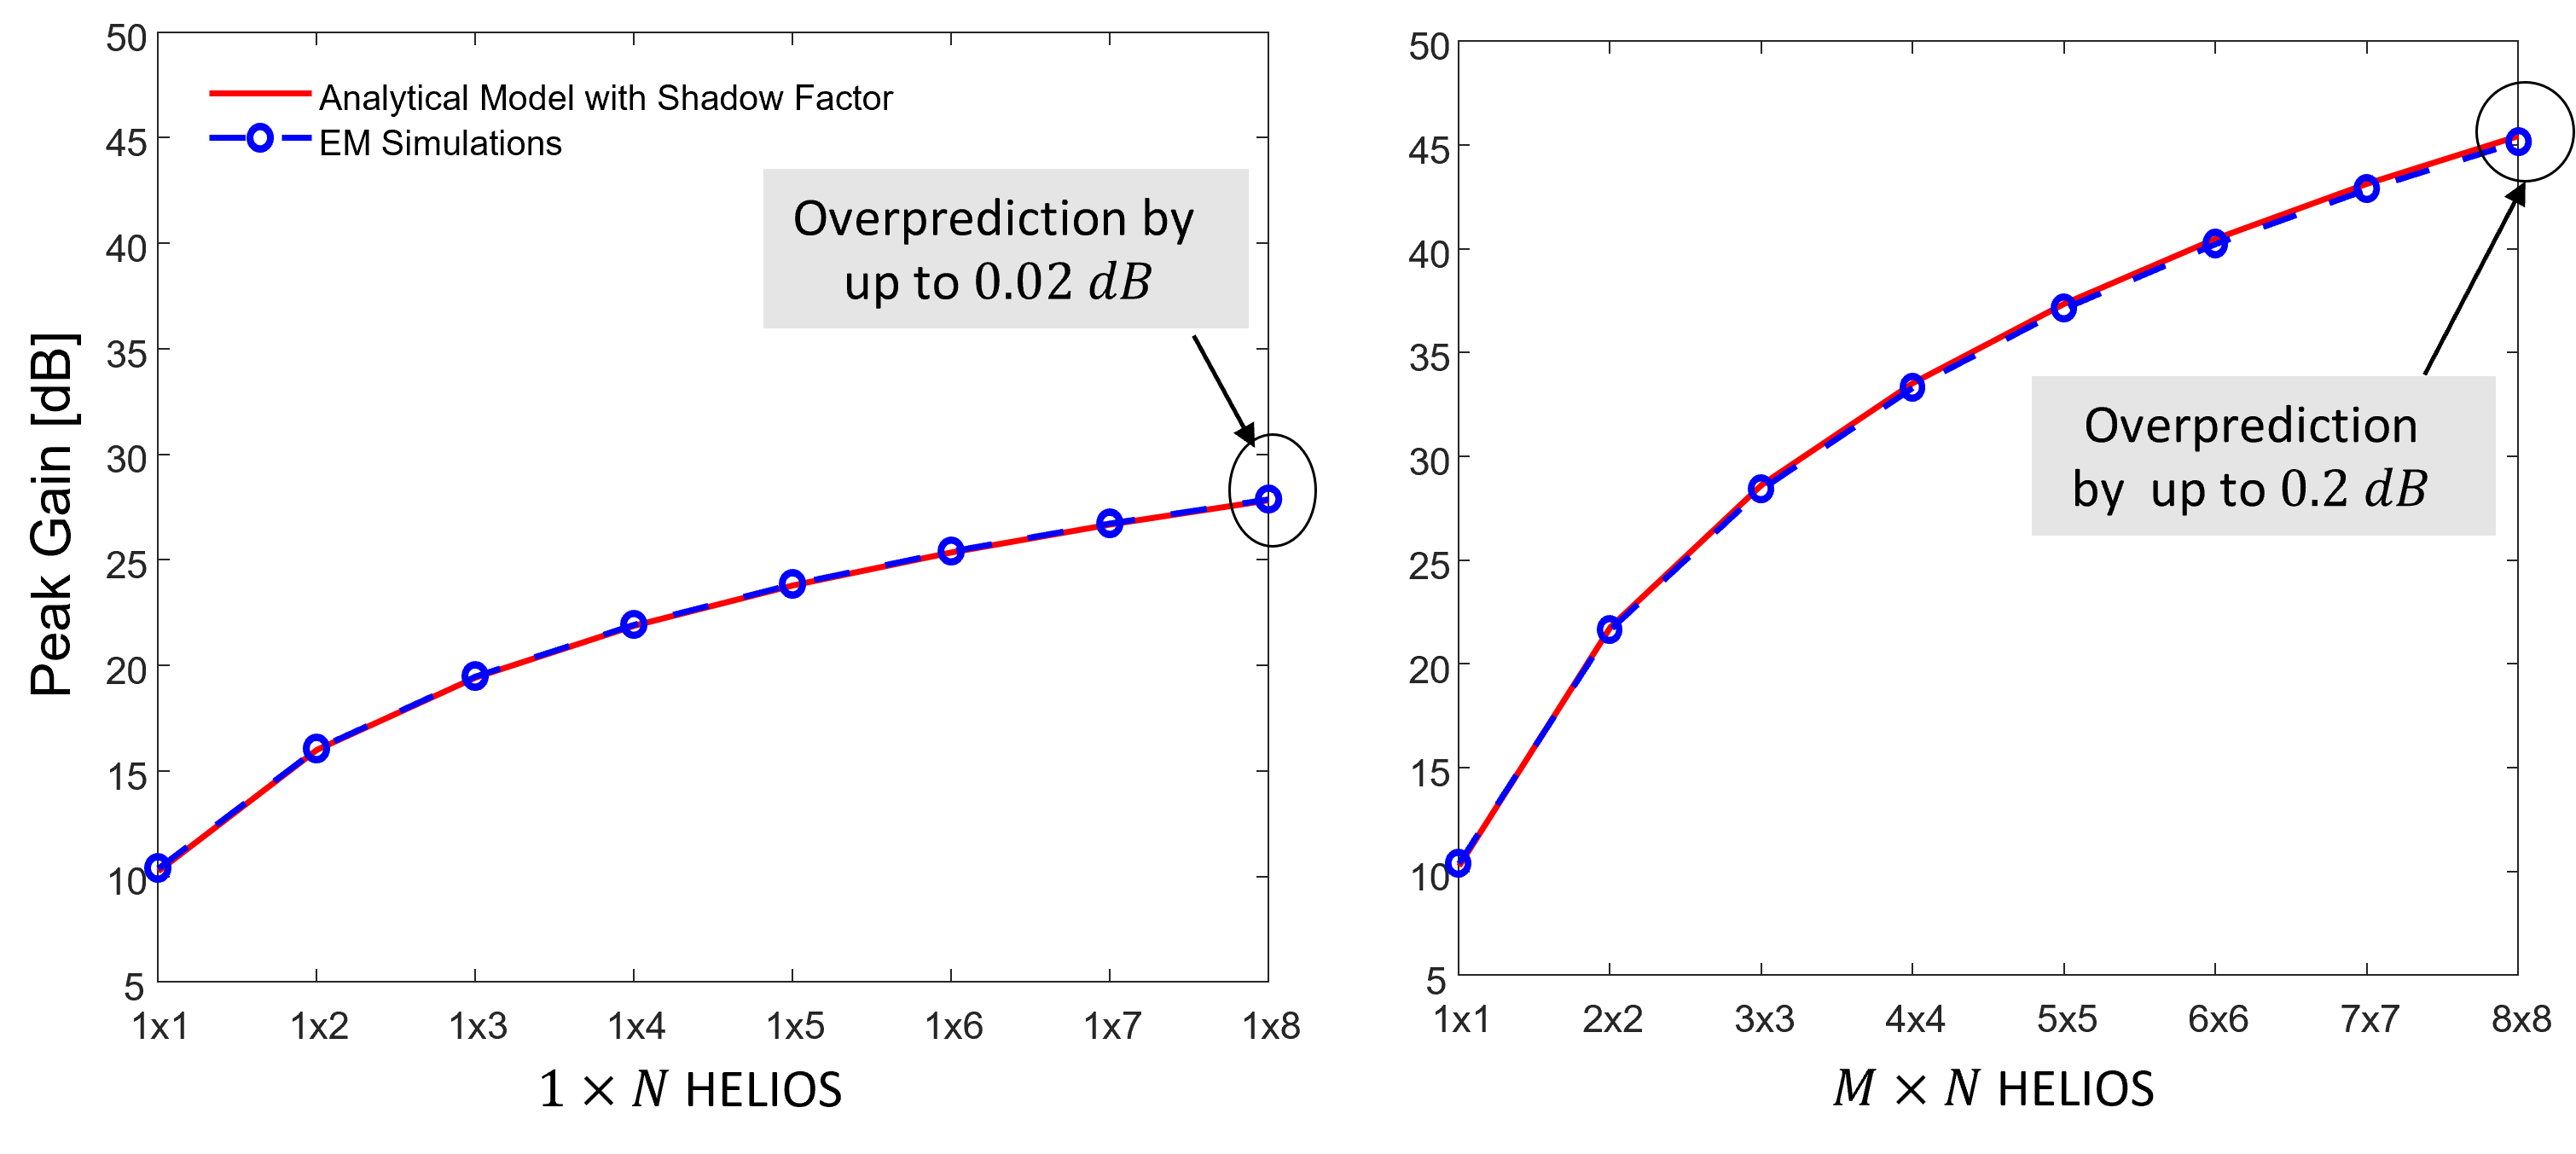
\includegraphics[width=1.0\linewidth]{images/Section 3 Images/Array_max_SR}
	\caption{Plot against HELIOS array and maximum gain between simulated and analytical model after the elimination of the shadowed region, highlighting the difference in maximum gain in $\si{\decibel}$ for the case when $a_{m,n}=b_{m,n}=\SI{10}{\centi\meter}$ and $\alpha_{m,n}=\beta_{m,n}=\num{10}^\circ$.}
	\label{fig:arraymax_SR}
\end{figure}
\section{Summary}
A brief overview of the prior section of \Cref{Simulation and Modeling of HELIOS Reflectors} is given in this section. The basic formulas that make up our analytical model are contained in \Cref{Eq:HELIOS_module} for an individual HELIOS module and by \Cref{Eq:HELIOS_array} for an array of HELIOS reflectors. \Cref{Improved Model using Inter-module Relations} improves our analytical model such that self-shadowing effects are accurately addressed. Important features are described, including the appearance of peak main lobe angles as determined by \Cref{HELIOS 2times beta}, and \Cref{HELIOS 2times alpha} and the beamwidth dependence of the module on dimensions $M$ and $N$ along the $y$ and $z$ axes, respectively. \Cref{Assessment of Differences between Simulations and Analytical Model} showcases the reflection behavior along different frequencies showing that the gain at higher frequencies is higher, but due to a more narrow reflection one needs to take more measures if one still wants to fairly distribute the reflection along a wider range of angles. Our comprehension is further enhanced by a brief comparison with the equations governing in \Cref{coordinate systems} showing the match between IRS and our analytical model.

The provided analytical model is actively used in \Cref{Performance Evaluation and Case Study} to forecast different communication channel features in various scenarios.
        % 
			%	\chapter{Section3}
\label{cha:Section3}
				\chapter{Performance Evaluation and Case Study}
\label{Performance Evaluation and Case Study}
The main focus of this section is to assess our analytical model compared to simulations as well as against IRS models.
We first examine computing time in detail in \Cref{Computing Time Analysis}, in which we compare the analytical model with EM simulation results. An urban case study similar to the recent work \cite{Helios} is presented in \Cref{Urban Case Study}. Here, we first assess the baseline performance using the FSPL channel model before moving on to channel models that integrate three IRS models (cf. \Cref{coordinate  systems}), and HELIOS (cf. \Cref{Analytical Modeling of HELIOS Modules}). At last, we also produce few case studies to strengthen our study on the HELIOS analytical model.
\section{Computing Time Analysis} \label{Computing Time Analysis}
The main goal of this section is to evaluate the computing efficiency between EM simulations using Ansys HFSS, see \Cref{sec:Simulation Methodology}, and our analytical model using Mathworks MATLAB \cite{Helios}. We note that the former is considered twice, one using \num{4}, and the other with \num{128} CPU cores, respectively. When it comes to computing time, analytical models typically do better than simulations, which motivated the work. Naturally, the performance of the analytical model does depend on the programming language and implementation. Regardless, because simulations require large amounts of processing power and intricate algorithms, their execution times may be longer.

\Cref{fig:flowchart_computingtime} provides a visual picture of our methodology and the ensuing data analysis. It shows the complete process, from HELIOS reflector paramterization, bistatic RCS calculation with different resolutions, computation, and computing time comparison. Based on this setup, we can assess the impact of this work's model against EM simulations. However, we note that other EM tools exist and could potentially provide the results with less computing time. Using more CPU cores or other models could also decrease the computing time. Similarly, the analytical model could in future be implemented in C/C++ for increase the computing time, too.

We use a Iron Python script that runs simulations with different $\alpha_{m,n}$,  $\beta_{m,n}$, $\theta_{Tx}$, and $\varphi_{Tx}$ parameters to carry out our experiment, where we use the computing time generated, with the help of tic and toc functions, to compare with the EM simulations of different simulation cores and our analytical model. The measured computing times are saved and then evaluated in MATLAB. There, we executed and measured the computing time of the analytical model for the HELIOS reflector with the identical set of parameters of the EM simulations.
\begin{figure}[H]
	\centering
	
\includegraphics[width=1\linewidth]{images/Section 4 Images/flowchart_computingtime}
	\caption{Methodological flowchart of this section's HELIOS computing time assessment comparing EM simulations and our analytical model for $m\in1,\dots,M$, $n\in1,\dots,N$.}
	\label{fig:flowchart_computingtime}
\end{figure}
\Cref{Table:Mean calculation time} contains the mean computing time for a HELIOS module with $a_{m,n}=b_{m,n}=\SI{10}{\centi\meter}$ and for two hundreds of these different combinations for the values in $\alpha_{m,n} \in [2:10]^\circ$, $\beta_{m,n} \in [2:10]^\circ$, $\theta_{Tx} \in [0:90]^\circ$, and $\varphi_{Tx} \in [0:90]^\circ$ in simulations. The values in the table is calculated for different angular resolutions. The bar graph representation of the same is given below in \Cref{fig:Computing_time_cores}, where the $x$-axis consists of different angular resolutions for different processors as color coded in the figure and the $y$ axis consists of mean computing time in \si{\second}. We make use of the speed-up factor $X$, to measure the performance gain from multi-core processors. It is the ratio of execution times between various processor configurations.

Notable speed-up factors are revealed in \Cref{fig:Computing_time_cores}, which offers insightful information, especially at a very high RCS resolution of $\num{0.5}^\circ$ for which the mean computing time of simulations takes several hundred seconds. The measured speed-up factors of the analytical model to EM simulation of \num{128} core, analytical model to EM simulation of \num{4} core , and \num{128} to \num{4} core EM simulations are roughly $8,740$, $14,681$, and \num{2.2}, respectively. This highlights the huge speed up of EM simulations by employing many CPU cores, on the one hand. On the other hand, however, simply switching to the analytical model massively outperforms this by reducing the computing time to just a fraction of a second, see \Cref{Table:Mean calculation time}. 
\begin{table}[H] % H -> dieses objekt wird genau da wo der code steht festgenagelt
	\caption{Mean computing time for a HELIOS module $(1 \times 1)$ with different angular resolutions of the bistatic RCS.}
	\label{Table:Mean calculation time}
	\centering
	\footnotesize
	\begin{tabular}{@{} >{\raggedleft\arraybackslash}p{2.5cm}| >{\raggedleft\arraybackslash}p{2.5cm} |>{\raggedleft\arraybackslash}p{2.5cm} |>{\raggedleft\arraybackslash}p{2.5cm} @{}}	
		\multicolumn{1}{c|}{\textbf{\begin{tabular}{@{}c@{}}Angular\\ Resolution \end{tabular}}} & \multicolumn{1}{c|}{\textbf{\begin{tabular}{@{}c@{}}Analytical \\ Model \end{tabular}}} & \multicolumn{1}{c|}{\textbf{\begin{tabular}{@{}c@{}}EM Simulations\\ (128 Core) \end{tabular}}} & \multicolumn{1}{c}{\textbf{\begin{tabular}{@{}c@{}}EM Simulations\\ (4 Core) \end{tabular}}} \\
		\hline
		$\num{2.0}^\circ$ & \SI{2.2}{\milli\second} & \SI{14.9}{\second} & \SI{32.3}{\second} \\
		\hline
		$\num{1.0}^\circ$ & \SI{6.1}{\milli\second} & \SI{34.8}{\second} & \SI{106.3}{\second}\\
		\hline
		$\num{0.5}^\circ$ & \SI{15.6}{\milli\second} & \SI{117.45}{\second} & \SI{400.4}{\second}
	\end{tabular}
\end{table}
\begin{figure}[H]
	\centering
	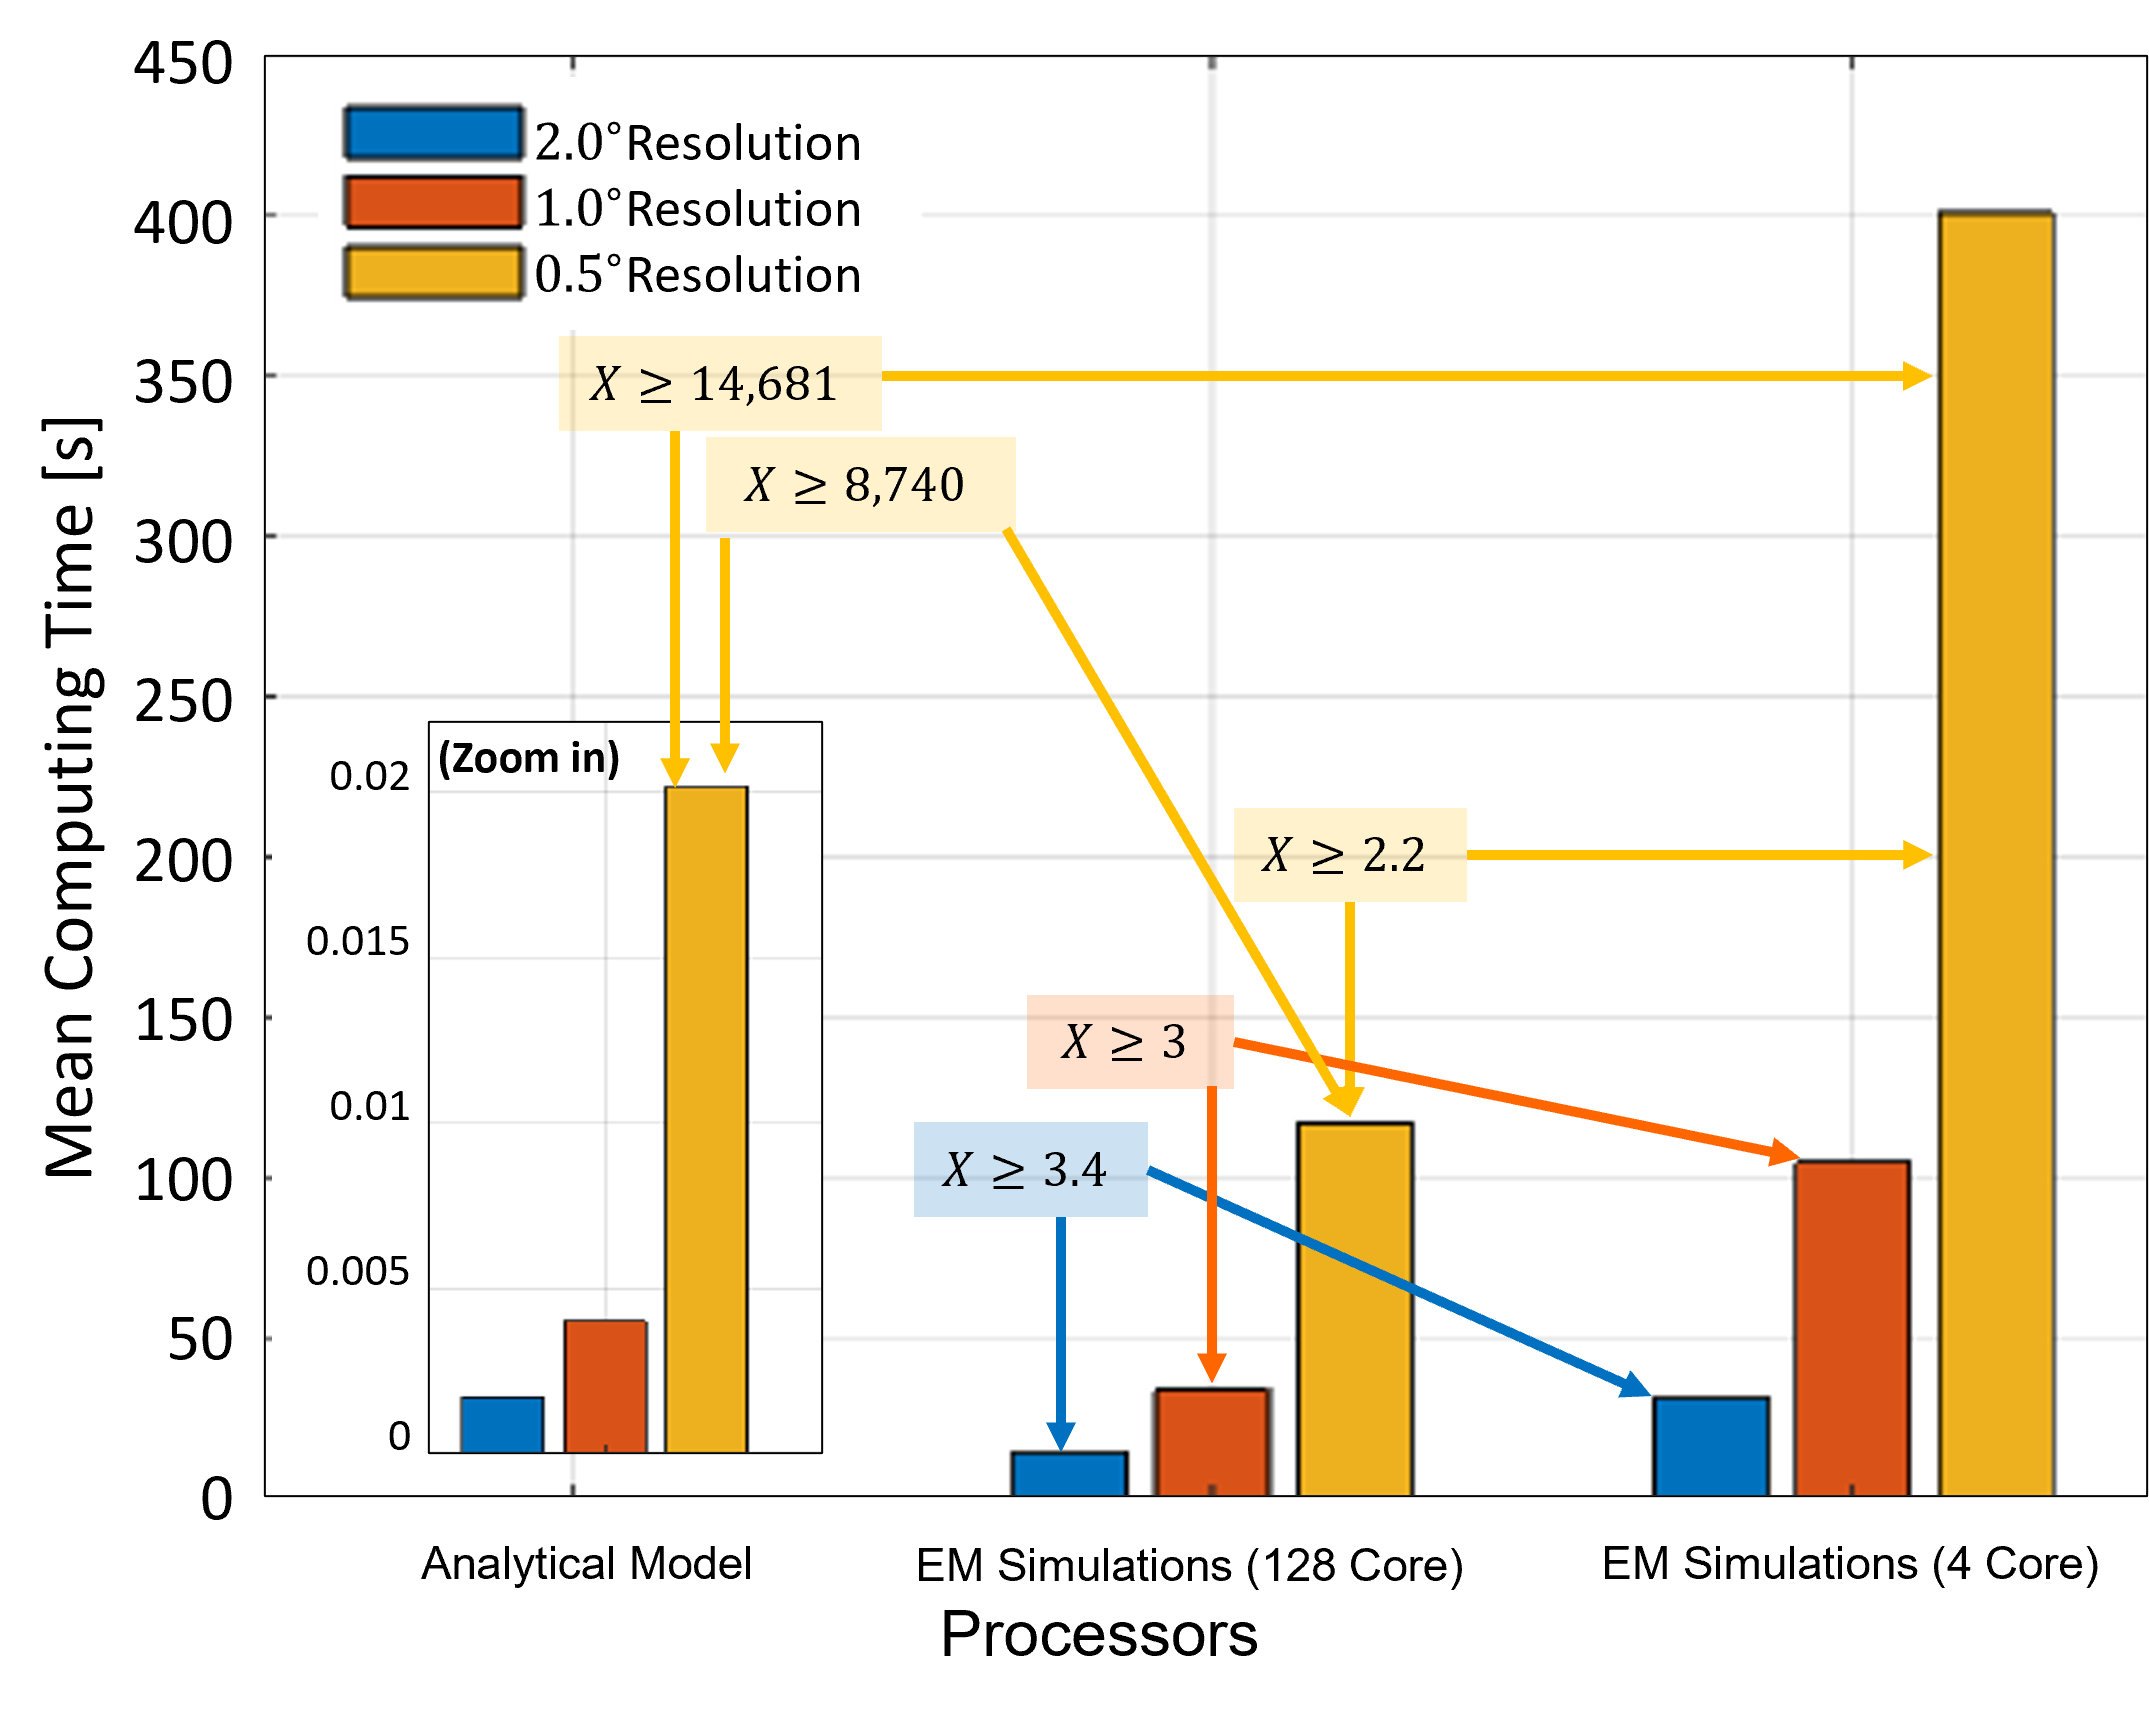
\includegraphics[width=0.75\linewidth]{images/Section 4 Images/Computing_time_cores}
	\caption{Mean computing time for a HELIOS module with different angular resolutions focusing on the speed-up factor X between different processors. Here, we find that the analytical model implementation is up to ca. $14,600$ times faster than the EM simulations with 4 core and ca. $8,740$ times faster than 128 core at $\num{0.5}^\circ$ angular resolution.}
	\label{fig:Computing_time_cores}
\end{figure}
\begin{figure}[H]
	\centering
	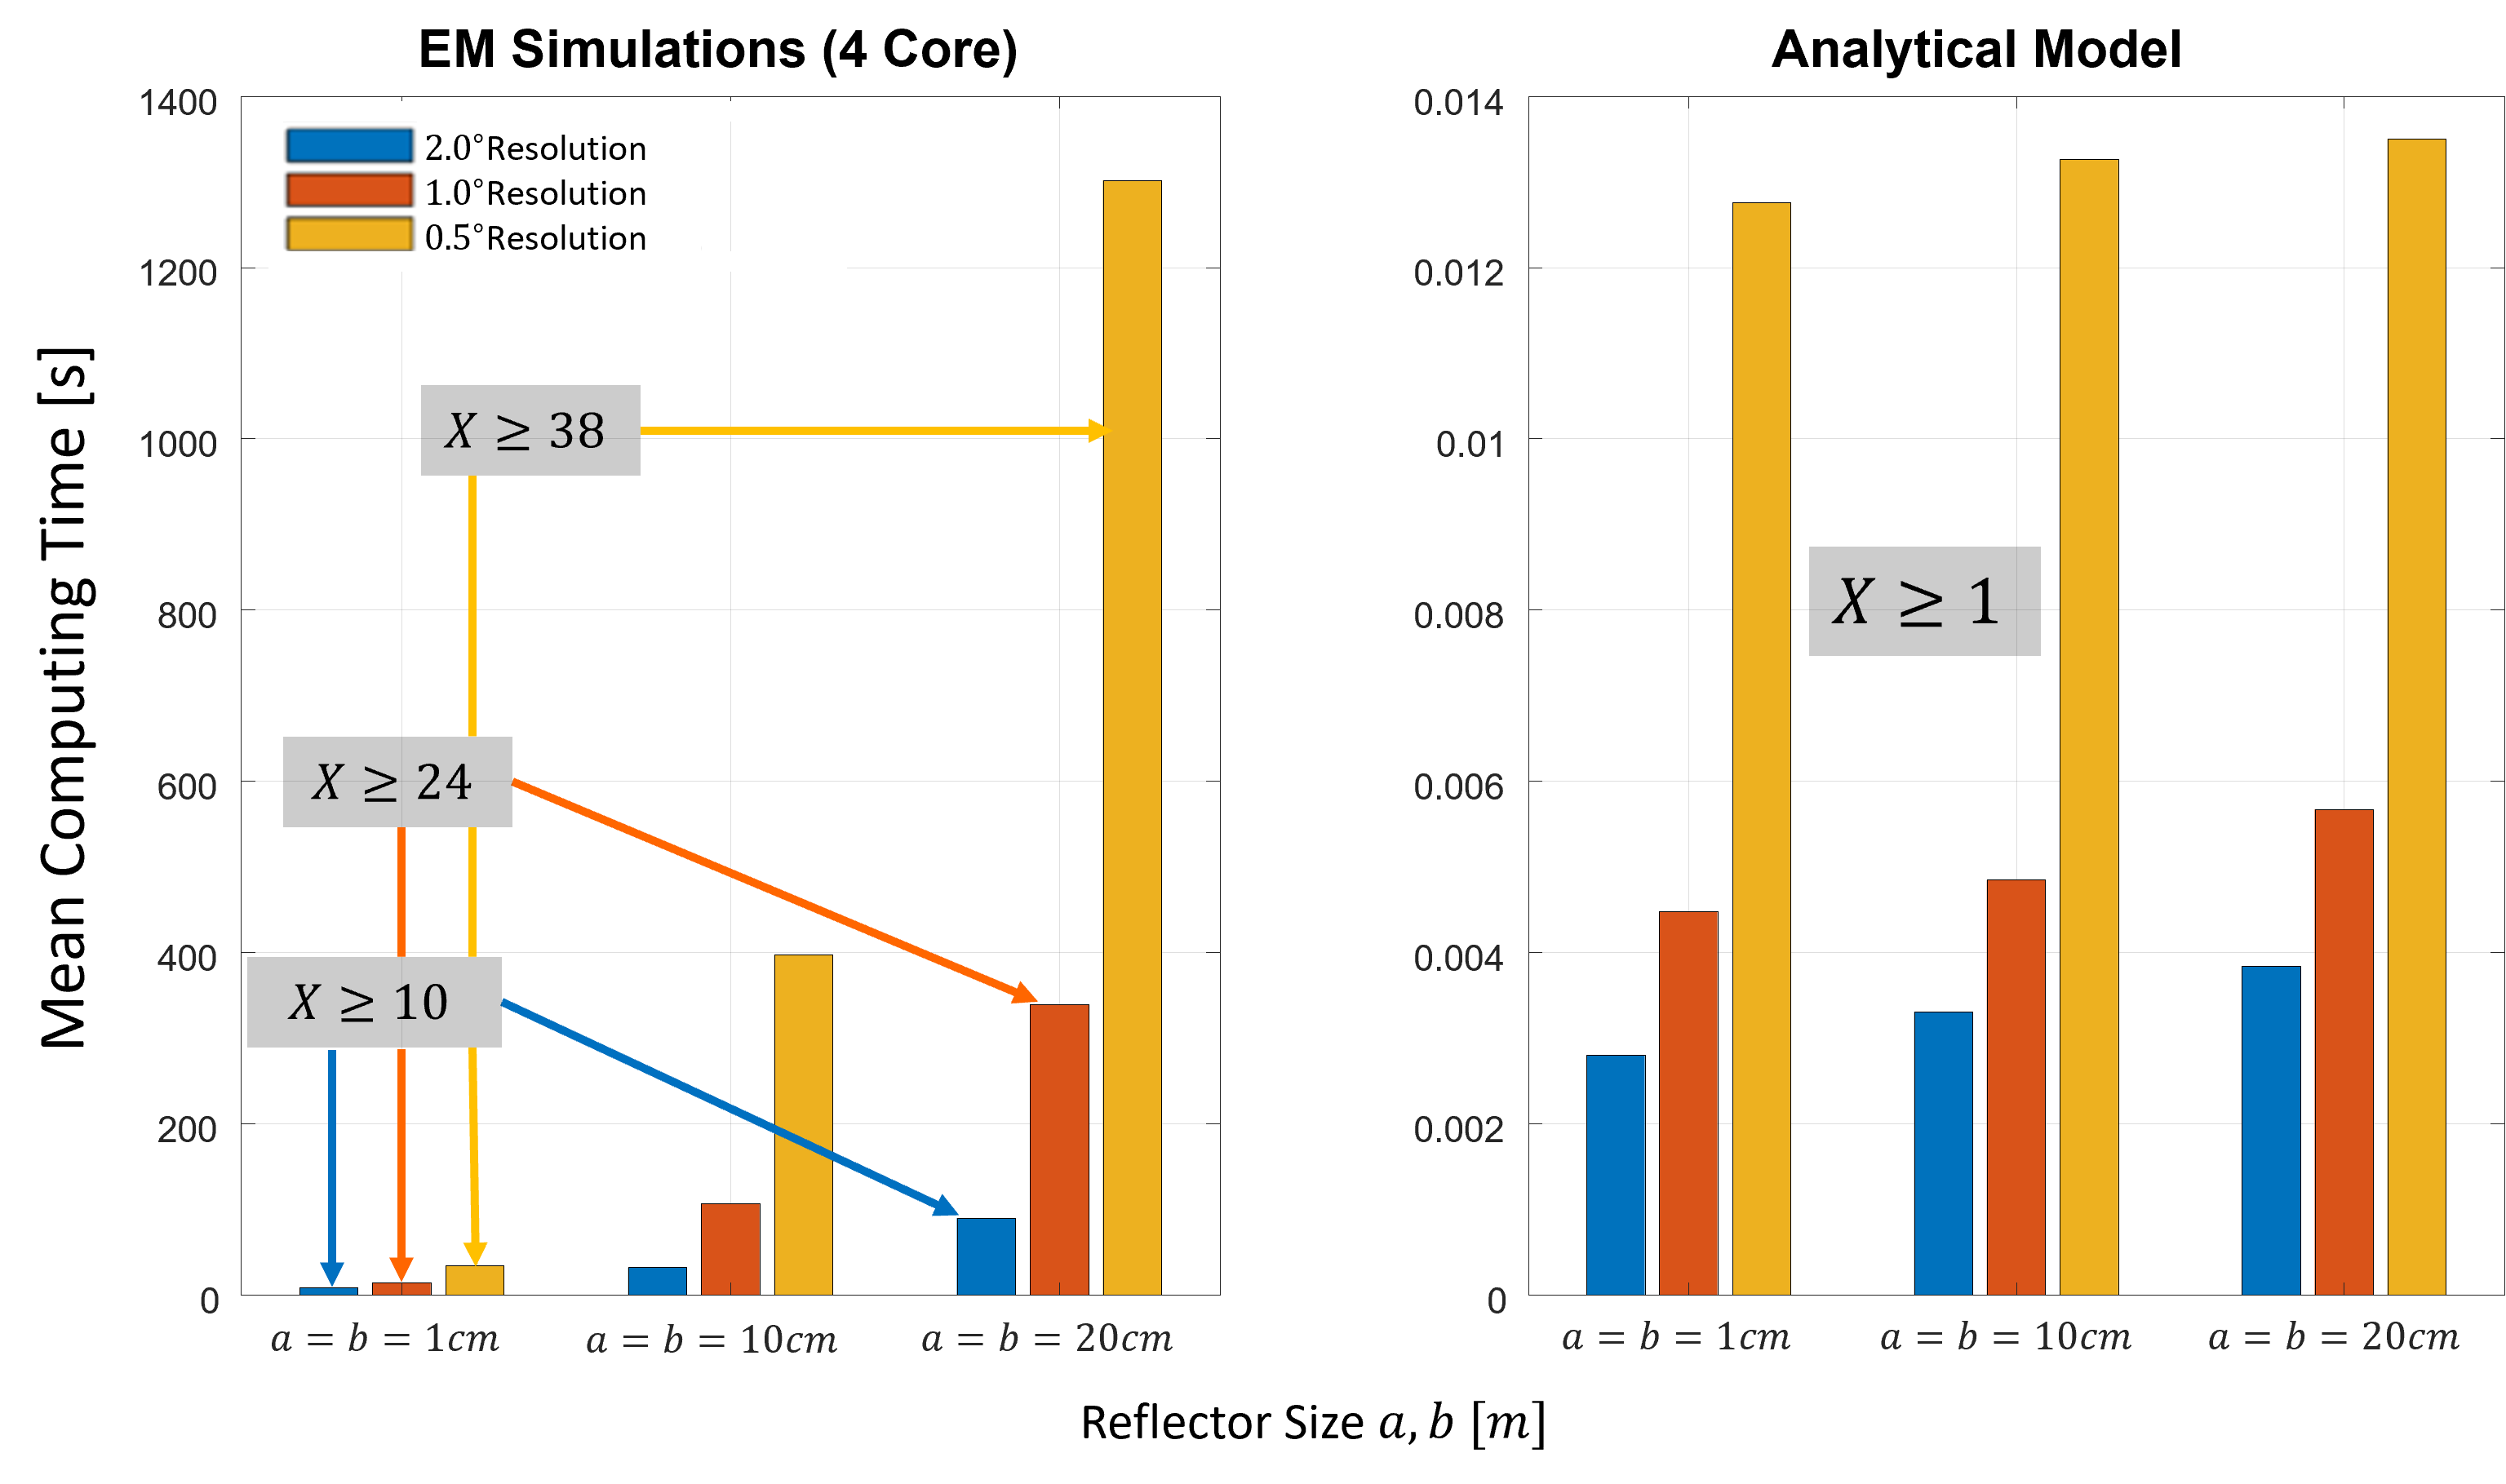
\includegraphics[width=0.85\linewidth]{images/Section 4 Images/Computing_time_size}
	\caption{Mean computing time analysis for a HELIOS module ($1 \times 1$) with varying angular resolutions highlighting the speed-up factors X between varying reflector sizes. Notably, as the reflector size increases, the mean computing time also increases in EM simulations with 4 core, but analytical model shows very little impact for varying sizes. }
	\label{fig:Computing_time_size}
\end{figure}
As can be noted, the results in \Cref{Table:Mean calculation time} corresponds to $a=b=\SI{10}{\centi\meter}$. Having considered the impact of the selected angular resolution of the RCS pattern, we move on to studying the impact of the reflector element size from $a=b=\SI{1}{\centi\meter}$ to $a=b=\SI{20}{\centi\meter}$ on the runtime. Similar to the previous paragraph, the results are provided below in \Cref{fig:Computing_time_size} and \Cref{Table:Mean calculation time2} for different HELIOS module dimensions $(1 \times 1)$.

\begin{table}[tb] % H -> dieses objekt wird genau da wo der code steht festgenagelt
	\caption{Mean computing time for different angular resolutions depicting variations for varying reflector sizes for a HELIOS module. We observe that the analytical model's computing time is independent to the reflector dimensions whereas the EM simulations scale poorly, thus demonstrating infeasibility for large reflecting surfaces size as expected for 6G, cf. case study in \Cref{Urban Case Study}.}
	\label{Table:Mean calculation time2}
	\centering
	\footnotesize
	\begin{tabular}{@{} c| >{\raggedleft\arraybackslash}p{3cm} |>{\raggedleft\arraybackslash}p{3cm} |>{\raggedleft\arraybackslash}p{3cm} @{}}	
		\multicolumn{1}{c|}{\textbf{\begin{tabular}{@{}c@{}}HELIOS Module\\ Dimensions \end{tabular}}} &
		\multicolumn{1}{c|}{\textbf{\begin{tabular}{@{}c@{}}Angular \\ Resolution \end{tabular}}} & \multicolumn{1}{c|}{\textbf{\begin{tabular}{@{}c@{}}Analytical \\ Model \end{tabular}}} &  \multicolumn{1}{c}{\textbf{\begin{tabular}{@{}c@{}}EM Simulations\\ (4 Core) \end{tabular}}} \\
		\hline
		\multirow{3}{*} \textbf{$a=b=\SI{1}{\centi\meter}$}
		& $\num{2.0}^\circ$ & \SI{2.9}{\milli\second} & \SI{8.4}{\second}  \\
		\cline{2-4}
		& $\num{1.0}^\circ$ & \SI{4.5}{\milli\second} & \SI{13.9}{\second}\\
		\cline{2-4}
		& $\num{0.5}^\circ$ & \SI{12.9}{\milli\second} & \SI{33.8}{\second}\\
		\hline
		\multirow{3}{*} \textbf{$a=b=\SI{10}{\centi\meter}$}
		& $\num{2.0}^\circ$ & \SI{3.4}{\milli\second} & \SI{31.7}{\second}  \\
		\cline{2-4}
		& $\num{1.0}^\circ$ & \SI{4.9}{\milli\second} & \SI{106.3}{\second}\\
		\cline{2-4}
		& $\num{0.5}^\circ$ & \SI{13.3}{\milli\second} & \SI{398.1}{\second} \\
		\hline
		\multirow{3}{*} \textbf{$a=b=\SI{20}{\centi\meter}$}
		& $\num{2.0}^\circ$ & \SI{3.9}{\milli\second} & \SI{89.6}{\second}  \\
		\cline{2-4}
		& $\num{1.0}^\circ$ & \SI{5.8}{\milli\second} & \SI{338.9}{\second} \\
		\cline{2-4}
		& $\num{0.5}^\circ$ & \SI{13.5}{\milli\second} & 1,309.3 \si{\second} \\
	\end{tabular}
\end{table}
A clear pattern can be observed underlining that the computing time of the EM simulations increased in tandem with reflector size. A significant speedup factor is seen in the bar graph of the \num{4}-core simulation as the reflector size increases from $a=b=\SI{1}{\centi\meter}$ to \SI{20}{\centi\meter}. In particular, there is a speedup factor of about \num{38}, \num{24}, and \num{10} for $\num{0.5}^\circ$, $\num{1}^\circ$, and $\num{2}^\circ$ resolutions, respectively. In contrast, we observe none of this for the analytical model, i.e., there is barely an impact on the computing time. Noticing from \Cref{Table:Mean calculation time2}'s mean computing time values for the analytical model, where very little effect regarding reflector size is observed, whereas, on the other hand, the values rise to 1,309.3 \si{\second} at $\num{0.5}^\circ$ angular resolution with $a=b=\SI{20}{\centi\meter}$. These results highlight the efficiency benefits made possible by the analytical model in a variety of scenarios, highlighting its superiority when it comes to managing bigger reflector sizes when compared to the simulation method.
\begin{table}[H] % H -> dieses objekt wird genau da wo der code steht festgenagelt
	\caption{Mean computing time for various HELIOS reflector array sizes (\num{1}$\times$\num{1}, \num{2}$\times$\num{2}, and \num{4}$\times$\num{4}) with different angular resolutions. A notable performance of our analytical model in \si{\milli\second} for an increase in reflector array demonstrates the advantage of the model to assess large-scale HELIOS configurations as compared to the simulation models. Parameters: $a_{m,n}=b_{m,n}=\SI{10}{\centi\meter}$.}
	\label{Table:Mean calculation time array}
	\centering
	\footnotesize
	\begin{tabular}{@{} c|>{\raggedleft\arraybackslash}p{2.5cm} | >{\raggedleft\arraybackslash}p{2.5cm} |>{\raggedleft\arraybackslash}p{2.5cm} |>{\raggedleft\arraybackslash}p{2.5cm} @{}}	
		\multicolumn{1}{c|}{\textbf{\begin{tabular}{@{}c@{}}HELIOS Reflector\\ Array \end{tabular}}} &
		\multicolumn{1}{c|}{\textbf{\begin{tabular}{@{}c@{}}Angular \\ Resolution \end{tabular}}} & \multicolumn{1}{c|}{\textbf{\begin{tabular}{@{}c@{}}Analytical \\ Model \end{tabular}}} & 
		\multicolumn{1}{c|}{\textbf{\begin{tabular}{@{}c@{}}EM Simulations\\ (128 Core) \end{tabular}}}& \multicolumn{1}{c}{\textbf{\begin{tabular}{@{}c@{}}EM Simulations\\ (4 Core) \end{tabular}}} \\
		\hline
		\multirow{2}{*} \textbf{\num{1}$\times$\num{1}}
		& $\num{2.0}^\circ$ & \SI{1.6}{\milli\second} & \SI{14.9}{\second} & \SI{31.7}{\second}  \\
		\cline{2-5}
		& $\num{1.0}^\circ$ & \SI{3.9}{\milli\second} & \SI{33.5}{\second} & \SI{106.4}{\second}\\
		\hline
		\multirow{2}{*} \textbf{\num{2}$\times$\num{2}}
		& $\num{2.0}^\circ$  & \SI{2.8}{\milli\second} & \SI{20.6}{\second} & \SI{77.9}{\second} \\
		\cline{2-5}
		& $\num{1.0}^\circ$ & \SI{11.2}{\milli\second} & \SI{49.8}{\second}  & \SI{282.8}{\second}\\
		\hline
		\multirow{2}{*} \textbf{\num{4}$\times$\num{4}}
		& $\num{2.0}^\circ$  & \SI{9.9}{\milli\second} & \SI{66.4}{\second} & \SI{503.9}{\second} \\
		\cline{2-5}
		& $\num{1.0}^\circ$  & \SI{28.6}{\milli\second} & \SI{197.7}{\second} & 1,574.6 \si{\second} \\
	\end{tabular}
\end{table}
\begin{figure}[tb]
	\centering
	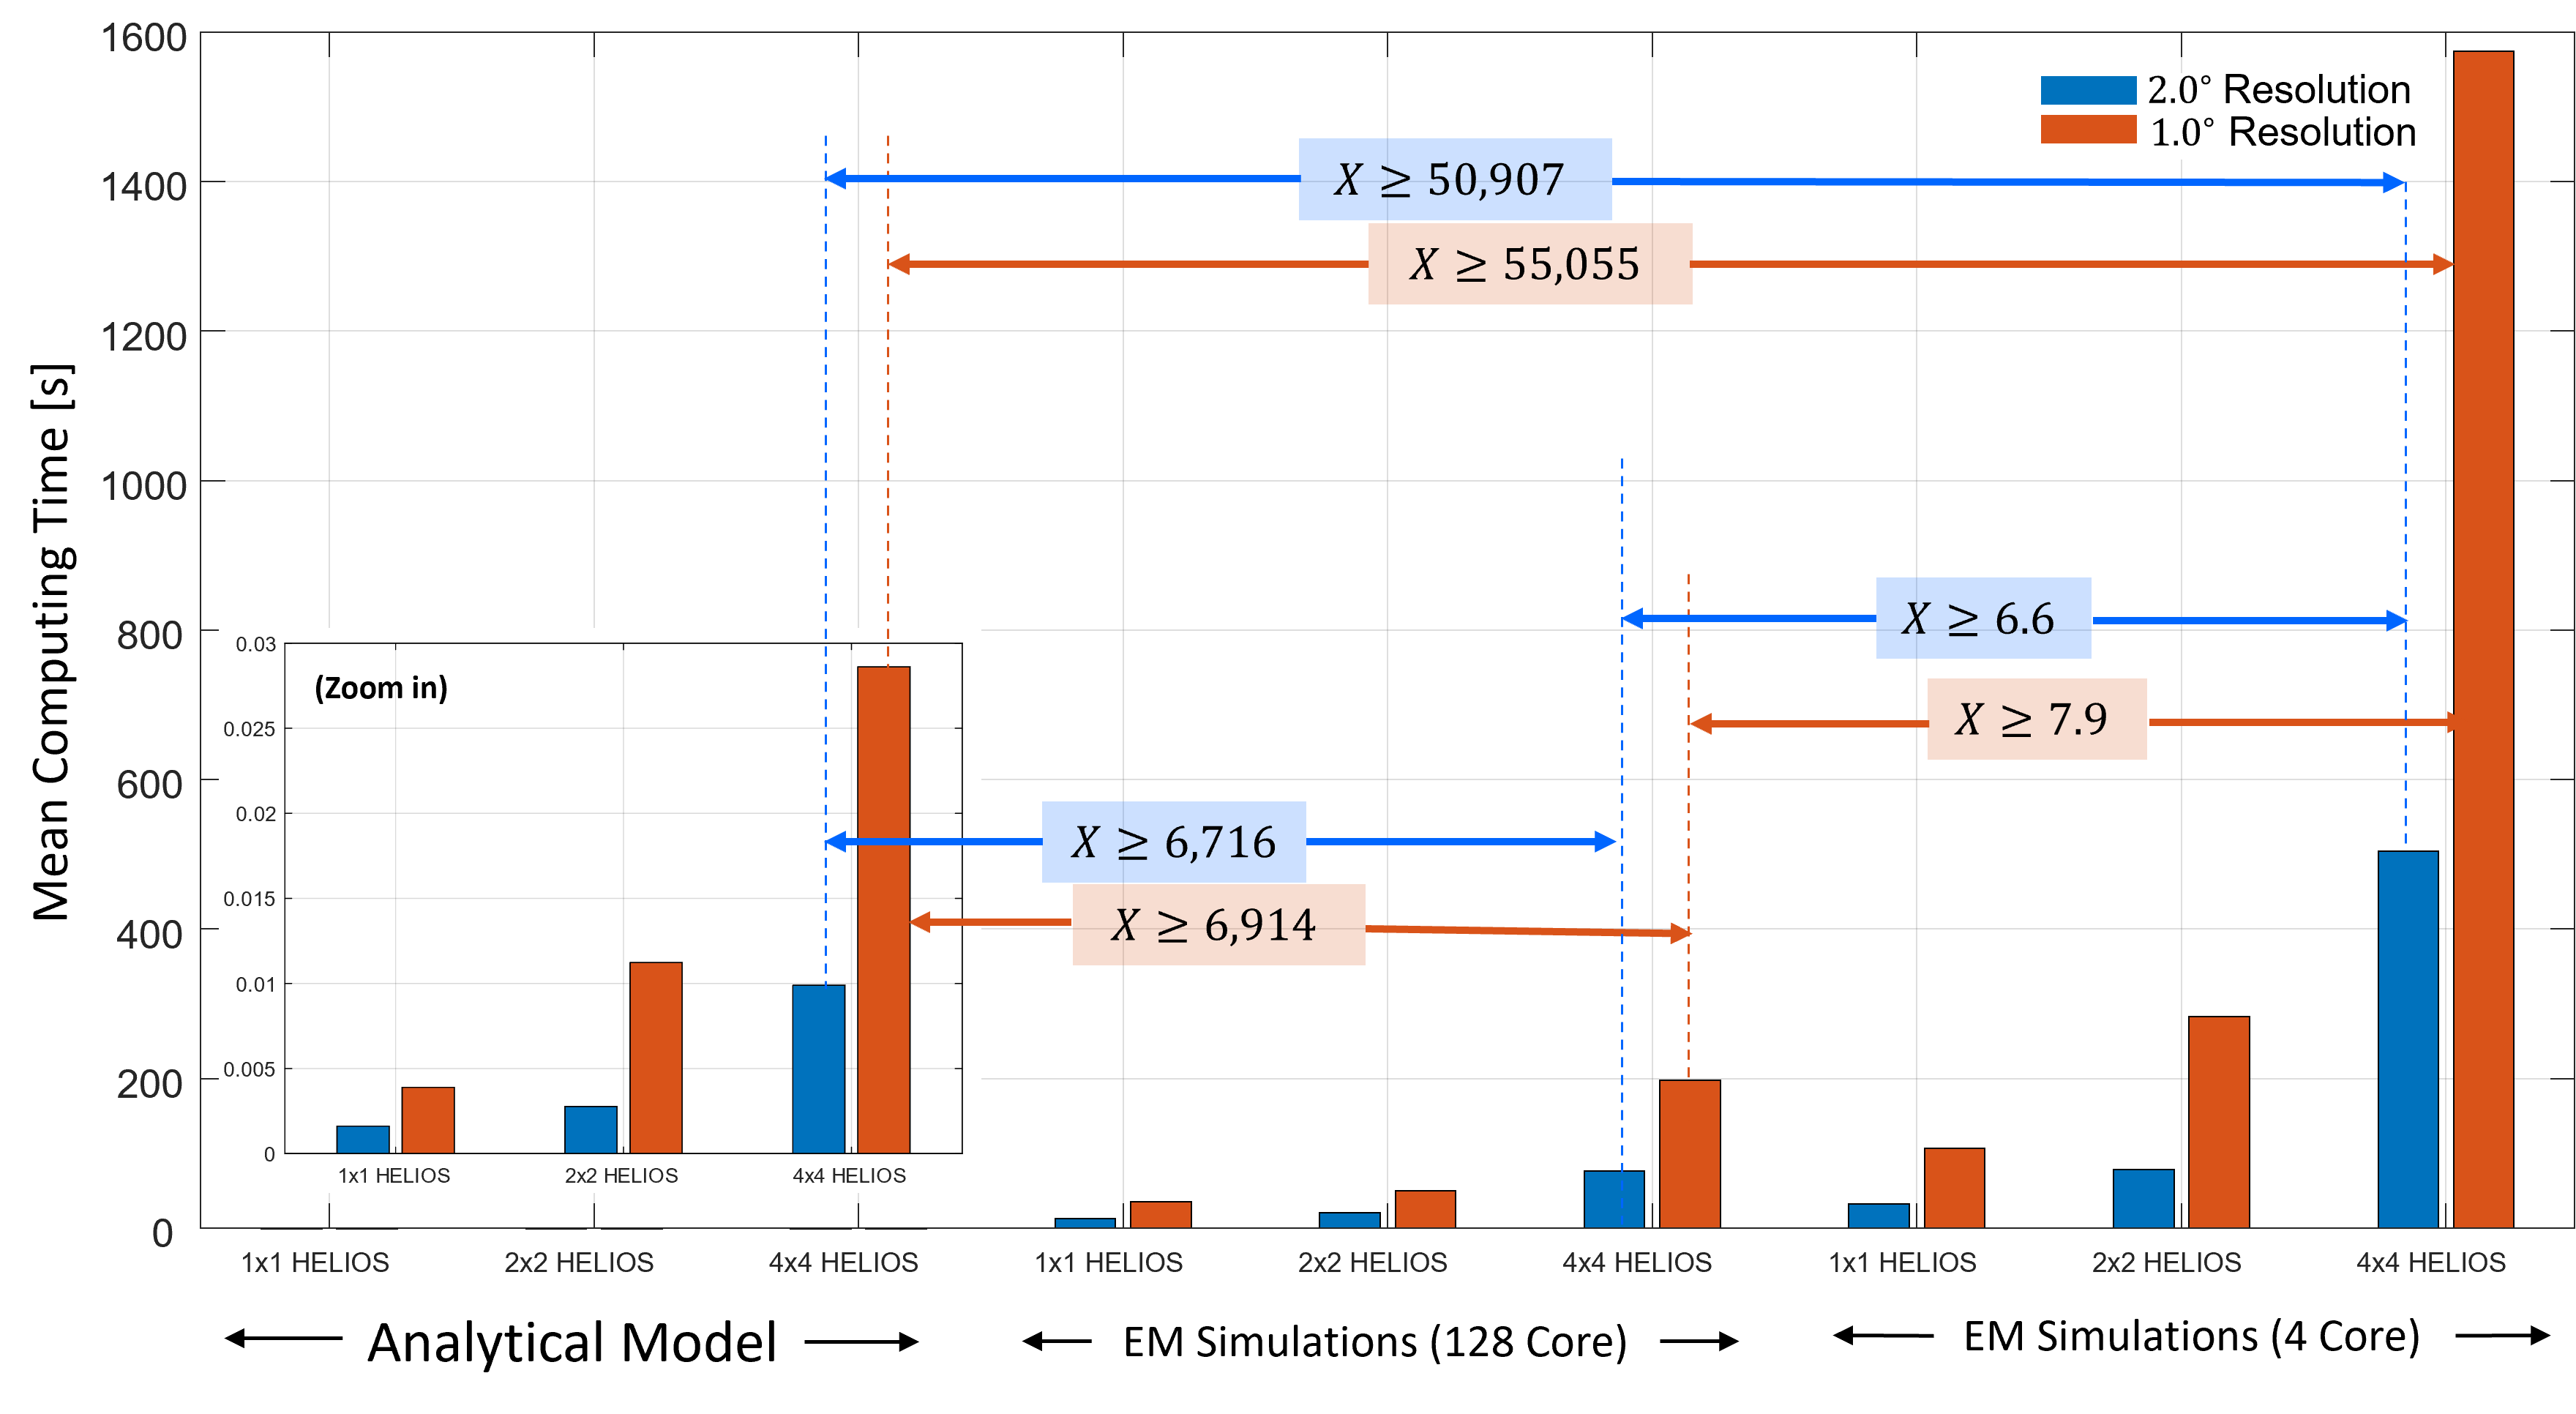
\includegraphics[width=1.0\linewidth]{images/Section 4 Images/Computing_time_resolution}
	\caption{Mean computing time analysis for various HELIOS reflector array sizes (\num{1}$\times$\num{1},\num{2}$\times$\num{2}, and \num{4}$\times$\num{4}) highlighting the speed-up factor X between different angular resolutions. A notable faster performance by the analytical model is observed for the large-scale array configurations as compared to that of the simulation model. }
	\label{fig:Computing_time_resolution}
\end{figure}
Moving on, we now investigate the computing time dynamics for various array sizes (\num{1}$\times$\num{1}, \num{2}$\times$\num{2}, and \num{4}$\times$\num{4}) using an analytical model and EM simulation of 4 core and 128 core configurations in our extended study. The mean calculation times for angular resolutions of RCS with $\num{1}^\circ$ and $\num{2}^\circ$ are given in \Cref{fig:Computing_time_resolution}, and \Cref{Table:Mean calculation time array}.  

Again, a similar pattern shows up for EM simulation architectures, indicating that computing time increases with array size. The measured speed-up factors at $\num{1}^\circ$ resolution show that the transitions from analytical model to \num{128} core EM simulations, analytical model core to \num{4} core EM simulations, and \num{128} core to \num{4} core EM simulations appear as 6,914, 55,055, and 7.9, respectively. It is interesting to note that this trend becomes stronger with decreasing angular resolution, leading to higher speedup factors. As a result, our analytical model performs substantially faster than simulation models, especially when there are a lot of array models available. This divergence highlights the efficiency boost for engineers using our proposed analytical model instead of EM simulations to assess large-scale HELIOS configurations.
\section{Urban Case Study}\label{Urban Case Study}
This section focuses on developing a deep comprehension of the urban scenario in \Cref{Urban Scenario Implementation} and forecasting various communication channel models in \Cref{Baseline Performance of FSPL Model}. By combining  the analytical model from \Cref{Analytical Modeling of HELIOS Modules} into practice in an urban setting, \Cref{Optimizing the HELIOS Geometry for Better Performance} and \Cref{Optimizing Connectivity with Different Reflector Positions} we optimize the configurations and assess the performance gains over the results with the original configurations in \Cref{Coupling Simulated and Analytical Reflection Pattern with Radar Realization}. The incorporation of this refined model into the IRS models explained in \Cref{coordinate systems} constitutes a fundamental component of our research, as seen in \Cref{Analyzing Urban Scenario for Different IRS Models}, where we also discuss two cases: beamformed to every possible position vs. one model which supports this fixed configuration similar to a passive reflector. A comparison study is carried out along with several case studies to thoroughly assess these models. Our investigation of the analytical model's effectiveness in actual urban communication situations is strengthened and expanded by these case studies. Lastly, in \Cref{Interpreting Different Channel Models} we extend our study to explore different channel models and analyze the performance gain.
\subsection{Urban Scenario Implementation}\label{Urban Scenario Implementation}
With this case study, we show how our HELIOS analytical model might be used in practice, for example in an urban environment, as shown in \Cref{fig:Scenario1}. The figure illustrates the location of the base station and clearly shows the distinction between Line-of-Sight (green-colored) and Non-Line-of-Sight (red-colored) zones. The two zones will be evaluated in \Cref{Baseline Performance of FSPL Model}. The judicious installation of a reflector on a nearby wall appears to be a good method to improve signal propagation and overcome potential obstructions in NLOS environments, as studied in \Cref{Coupling Simulated and Analytical Reflection Pattern with Radar Realization} and \Cref{Optimizing the HELIOS Geometry for Better Performance}.
\begin{figure}[H]
	\centering
	\includegraphics[width=1.0\linewidth]{images/Section 4 Images/Scenario1}
	\caption{Illustration of urban scenario \cite{Helios} with a well-aligned LOS path from the base station to the reflector center. The scenario highlights the reflections from the \SI{3}{\meter} $\times$ \SI{3}{\meter} reflector mounted on the building to serve the NLOS south street canyon region, as depicted.}
	\label{fig:Scenario1}
\end{figure}

By rerouting signals into our area of interest, i.e., south street canyon region, this reflective surface maximizes communication potential. \Cref{Table:Urban case study} provides a detailed description of the scenario's particulars, which are identical to \cite{Helios}. The base station, which uses \SI{100}{\mega\hertz} of bandwidth and operates at a frequency of \SI{28}{\giga\hertz}, is mounted on the corner of a large $ \SI{100}{\meter} \times  \SI{100}{\meter} \times \SI{20}{\meter}$ building complex at a height of \SI{10}{\meter}. According to \Cref{Table:Urban case study}, the parameters $\varphi_{BS}$ and $\theta_{BS}$ guide the orientation of the base station to precisely target the center of a designated \SI{3}{\meter} $\times$ \SI{3}{\meter}  mounting area for different reflectors under test, always mounted at a height of \SI{5}{\meter} above ground. The scenario takes place at a street crossing, where the transmitted signal from the base station is in a well-aligned LOS path to the reflector center. In a grid with \SI{1}{\meter} spacing, the receiver grid is uniformly positioned at a height of \SI{1.5}{\meter} and stretches up to \SI{60}{\meter} from the crossing point. Most notably, this simulation includes channels between the transmitter and thousands of potential receiver positions, offering a thorough grasp of the model's functionality in an actual metropolitan setting.
\begin{table}[tb] % H -> dieses objekt wird genau da wo der code steht festgenagelt
	\caption{Key parameters and their values at transmitter, receiver, and the reflector applicable to the urban street corner scenario at \SI{28}{\giga\hertz} frequency.}
	\label{Table:Urban case study}
	\centering
	\begin{tabular}{>{\centering\arraybackslash}m{2cm}|>{\centering\arraybackslash}m{7cm}|>{\centering\arraybackslash}m{5cm}}
		& \textbf{Parameter} & \textbf{Values}\\
		\hline
		\multirow{5}{*} \textbf{$P_{Tx}$}
		& Power transmitted & \SI{20.3}{\decibel}m\\
		\cline{2-3} 
		& $G_{Tx}$ & \SI{19.7}{\decibel}i\\
		\cline{2-3}
		& Position $(x,y,z)$ & (\SI{309.9}{\meter}, \SI{170.1}{\meter}, \SI{10.0}{\meter})\\
		\cline{2-3} 
		& $r_{Tx, Ref}$ & \SI{115.0}{\meter}\\
		\cline{2-3}
		& Beam orientations $(\varphi_{BS}, \theta_{BS})$ & ($\num{80.17}^\circ,\num{-2.46}^\circ $)\\
		\hline
		\multirow{8}{*} \textbf{Receiver}
		& Antenna Gain & \SI{19.7}{\decibel}i\\
		\cline{2-3} 
		& Position grid center $(x,y,z)$  & (\SI{309.9}{\meter}, \SI{170.1}{\meter}, \SI{10.0}{\meter})\\
		\cline{2-3}
		& Grid size   $x$-$z$-plane & \SI{120.0}{\meter} $\times$ \SI{120.0}{\meter}\\
		\cline{2-3} 
		& Grid density & \SI{1.0}{\meter}\\
		\cline{2-3} 
		& $r_{Ref, Rx}$ range & [\num{3.5}: \num{102.6}] \si{\meter}\\
		\cline{2-3}
		& Receiver Sensitivity $S_{Rx}$ & \SI{-83.5}{\decibel}m\\
		\cline{2-3}
		& Angle Ranges towards street crossing/Reflector $(\varphi_{UE}, \theta_{UE})$	&$ \varphi_{Rx}:[\num{-85.6}^\circ: \num{87.3}^\circ]$ and
		$\theta_{Rx}:[\num{-87.1}^\circ : \num{86.0}^\circ]$\\
		\hline
		\multirow{3}{*} \textbf{Reflector}
		& Footprint size $x$-$z$-plane & \SI{3.0}{\meter} $\times$ \SI{3.0}{\meter}\\
		\cline{2-3} 
		& Reflector Array Configuration & \num{1} $\times$ \num{32}\\
		\cline{2-3}
		& Midpoint of Reflector Backplane  $(x,y,z)$ & (\SI{195.0}{\meter}, \SI{170.0}{\meter}, \SI{5.0}{\meter})\\
	\end{tabular}
\end{table}
One thing to notice in the example is that there is a black area that is not expected to be covered via the reflector. A case study in \Cref{Optimizing Connectivity with Different Reflector Positions} will assess the impact of moving away from the reflector mounting position used in the paper \cite{Helios}.

After an initial assessment of the mmWave connectivity around the street crossing in \Cref{Urban Case Study}, the connectivity gains of two HELIOS reflector deployments are considered in this section. Like in the original paper, a "narrow beam" HELIOS configuration with slope angles being constant, constitutes the first reflector deployment option. In contrast, the "broad beam" HELIOS configuration results from our exploration of a wider range of slope angles throughout the array. Both options are depicted in \Cref{fig:beams}. The two cases are described as such:
\begin{itemize}
	\item \textbf{Narrow beam HELIOS}: Slope $\alpha_{1}=...=\alpha_{32}=\num{27.6}^\circ$, and $\beta_{1}=...=\beta_{32}=0^\circ$.
	\item \textbf{Broad beam HELIOS}: Slope angle variation in steps of $\num{2.5}^\circ$ with $\alpha_{1},....,\alpha_{32} \in [17.6^\circ:32.6^\circ]$, $\alpha_{2}, \alpha_{1}= \num{17.6}^\circ$, $\alpha_{6}, ...., \alpha_{3}=  \num{20.1}^\circ$, $\alpha_{11}, ...., \alpha_{7}= \num{22.6}^\circ$, $\alpha_{17}, ...., \alpha_{12}= \num{25.1}^\circ$, $\alpha_{23}, ...., \alpha_{18}= \num{27.6}^\circ$, $\alpha_{28}, ...., \alpha_{24}= \num{30.1}^\circ$, and $\alpha_{32}, ...., \alpha_{29}= \num{32.6}^\circ$.\\
	 Similar to narrow beam reflector configuration $\beta_{1}= ...= \beta_{32}=0^\circ$.
\end{itemize}
\begin{figure}[tb]
	\centering
	\includegraphics[width=1.0\linewidth]{images/Section 4 Images/beams}
	\caption{Top view illustration of original "narrow beam" and "broad beam" configuration for \num{1} $\times$ \num{32} HELIOS. We note that due to the symmetry of the original work, we adopt the flipped indices order.}
	\label{fig:beams}
\end{figure}
The visual summary of our methodology is presented in \Cref{fig:Scenario2}, which provides a top-view portrayal of the scenario that we are studying. The outage region, or regions where the reflectors are unable to provide coverage, is depicted in \Cref{fig:Scenario2}. As in \Cref{fig:Scenario1}, the buildings are represented by gray areas. Our main goal in this illustration is to cover the area such that the received power is greater than the designated receiver sensitivity threshold, i.e., as many potential UE positions in the south street canyon shall be able to connect to the network despite being in NLOS.

\begin{figure}[H]
	\centering
	\includegraphics[width=1\linewidth]{images/Section 4 Images/Scenario2}
	\caption{Sample illustration of received power analysis in the urban scenario to highlight the region of interest, i.e., south street canyon, where received power is greater than receiver sensitivity and the outage region.}
	\label{fig:Scenario2}
\end{figure}
\subsection{Baseline Connectivity Using LOS Channel Models}\label{Baseline Performance of FSPL Model}
Here we apply the FSPL model from \Cref{Free space propagation model} to estimate the received signal strength in the LOS regions of the selected scenario. We note that the NLOS regions will be assumed to have infinite path loss. After mounting of a reflecting surface, e.g., HELIOS or IRS, we also use the radar equation \Cref{Eq:HELIOS_array} to predict the receive power level at all UE positions, i.e., NLOS and LOS positions. 

\Cref{FSPL_delta}, which represents the excess path loss components that are then removed from the comprehensive path loss equation, explains the difference between the chained path loss equations, i.e., $PL_{Tx,Ref} \circ  PL_{Ref,Rx}$ (see \Cref{FSPLChained}).  This equation provides a clear and concise illustration of the virtual LOS situation by directly representing the radar path.
\begin{equation}\label{FSPLChained}
	\begin{aligned}
		PL_{FSPL_{Radar}}(r_{Tx,Ref},r_{Ref,Rx},f,\sigma_{Meta},G_{Tx}, G_{Rx})&=PL_{FSPL}(G_{Tx}, r_{Tx,Ref},f)+PL_{FSPL}(G_{Rx}, r_{Ref,Rx},f)+\\ &\sigma_{Meta}-\Delta D_{ChainnedFSPL},
	\end{aligned}
\end{equation}
where
\begin{equation} \label{FSPL_delta}
	\Delta D_{ChainedFSPL}= 10\cdot log_{10}(4 \cdot \pi)- 20\cdot log_{10}(c)+20\cdot log_{10}(f)
\end{equation}
\Cref{FSPL_delta} is already incorporated in \Cref{FSPL_dB_Radar}. Using this equation, we refer the reader to \Cref{fig:FSPL_Radar} for a brief comparison between the power level prediction for an arbitrary scenario assuming $\sigma_{Meta}=\SI{0}{\decibel}$ and the reflector location to be $r_{Tx, Ref}=\SI{50}{\meter}$ (see \Cref{Radar-Cross-Section and Radar Equation}).
\begin{figure}[H]
	\centering
	\includegraphics[width=0.75\linewidth]{images/Section 4 Images/FSPL_Radar}
	\caption{Comparison between predicted path loss of FSPL and radar equations over the total distance between Tx and Rx. For the radar equation curve, we assume LOS connectivity for the first \SI{50}{\meter}. Thereafter, it holds $\sigma_{Meta}=\SI{0}{\decibel}$, $r_{Tx, Ref}=\SI{50}{\meter}$ and $r_{Ref, Rx}=r_{Tx, Rx}$.}
	\label{fig:FSPL_Radar}
\end{figure}
A notable shift of about \SI{50}{\decibel} is observed at the reflector location $r_{Tx, Ref}=\SI{50}{\meter}$. Referring back to \Cref{Table:standard_sigma_values}, a car normally provides a $\sigma_{Meta}$ value of about \SI{20}{\decibel}. The observed shift at the reflector position is further reduced to about \SI{30}{\decibel} when considered. Using geometries explicitly tailored to achieve high RCS, such as reflecting surfaces, particularly by scaling the reflecting surface area, such scenarios as considered in the context of \Cref{fig:FSPL_Radar} can be overcome such that a reflector path can provide virtual LOS connectivity. 
\subsection{Analyzing Connectivity Enhancement by HELIOS Reflectors}\label{Coupling Simulated and Analytical Reflection Pattern with Radar Realization}
We now move on and assess the performance after mounting the narrow beam and broad beam HELIOS reflectors, respectively. For this purpose, we now put the radar equation to use, cf. \Cref{Eq:HELIOS_array}, For $\sigma_{Meta}$, we either substitute our analytical model or the simulation results, see \Cref{fig:urbanscenario_analy_sim}.

Initially, we verify the behavior of our analytical model through a comparison with simulation-based RCS patterns taken from \cite{Helios}. Our results are illustrated visually in  \Cref{fig:urbanscenario_analy_sim}, which includes heatmaps for both narrow and broad beams. The heatmaps, in particular, highlight that the coordinates $(\theta_{Rx}, \varphi_{Rx})=(\num{-2.5}^\circ, \num{-25.75}^\circ)$ are where the highest peak occurs and are in match.
\begin{figure}[H]
	\centering
	\includegraphics[width=0.9\linewidth]{images/Section 4 Images/urbanscenario_analy_sim}
	\caption{RCS comparison heatmaps between the HELIOS analytical model and EM simulation results in urban scenarios highlighting the gain behavior for both narrow and broad beams. Notably, a concentrated single lobe appears in narrow beam HELIOS, as the beams are focused in one direction at $(\theta_{Rx}, \varphi_{Rx})=(\num{-2.5}^\circ, \num{-25.75}^\circ)$, whereas with broad beam HELIOS, we observe multiple side lobes.}
	\label{fig:urbanscenario_analy_sim}
\end{figure}
The narrow beam HELIOS yields a peak gain of \SI{54.6}{\decibel} with EM simulations, whereas \SI{52.9}{\decibel} with the analytical model. Since it closely matches the simulated results, this consistency highlights the precision and dependability of our analytical method. As with broad beam HELIOS, our analytical model records a peak gain of \SI{40.7}{\decibel}, whereas the simulation model records a little higher value of \SI{48.7}{\decibel}. The overall trend shows an agreement between our analytical predictions and the simulated results, despite subtle differences in the magnitudes at the above-discussed angles. Since it faithfully reflects the simulation's observations of the larger beams' performance characteristics, this parallelism adds even more support to the validity of our analytical model.

Complementing the previous paragraph, we take a look at \Cref{fig:urbanscenario_analy_sim_ECDF} depicting the ECDFs of the previously discussed RCS heatmaps. They underline that there is a fundamental match, e.g., in terms of mean value: For the narrow beam configuration, the mean gain difference is \SI{2.8}{\decibel} with the analytical model predicting less reflection power than the EM simulations. This difference increases up to \SI{9.7}{\decibel} for the broad beam HELIOS. Whereas this suffices that the analytical model does not overpredict, we note that the ECDFs are not always weaker than the ones of the simulations. However, this shows that overprediction is rare. Like our investigation in \Cref{Analytical Modeling of HELIOS Modules}, this suggests that our analytical model provides a conservative estimate, even when scaling the reflecting surface to such large dimensions which potentially pushes analytical models and EM simulation tools to the limit.

In this section, we assess the impact on the received power for UEs located in the far-field region of the reflector under test. To make this transparent in our result figure, we highlight the near-field zone \cite{Neubauer1997, hansen1988spherical}, as defined by \Cref{Near-field} below, as a white color coding.
\begin{figure}[H]
	\centering
	\includegraphics[width=0.7\linewidth]{images/Section 4 Images/urbanscenario_analy_sim_ECDF}
	\caption{ECDF vs gain at the reflector plot for narrow and broad beam HELIOS highlighting the difference along the mean between simulated results and analytical model in \si{\decibel}. The parameters are considered from \Cref{Table:Urban case study} at \SI{28}{\giga\hertz} frequency. }
	\label{fig:urbanscenario_analy_sim_ECDF}
\end{figure}
Given $M\cdot a=N\cdot b=\SI{3}{\meter}$, the near-field region extends up to \SI{8.4}{\meter} in this case study. 
\begin{equation} \label{Near-field}
	r_{Ref, Rx} \leq \frac{\max \left( \left( M \cdot a \right)^2, \left( N \cdot b \right)^2 \right)}{\lambda}
\end{equation}
By integrating the HELIOS analytical model into our urban environment, we can predict the RCS towards each potential UE position and therefore also determine the expected receive power level. These heatmaps in \Cref{fig:urbanscenario_originalvalues} show the maximum power received which is expressed in \si{\decibel}m and the RCS gain which is measured in \si{\decibel} from the reflector into the receiver grid. The method for calculation of maximum power received is given by $P_{Rx_{Max}}= max(P_{Rx_{LOS}}, P_{Rx_{Radar}})$, where the maximum power received with LOS and radar channel modeling is considered.

From the figure below, narrow beam HELIOS gives a peak gain of about \SI{15.4}{\decibel}, whereas \SI{11.2}{\decibel} with broad beam HELIOS. It appears from the figure that power is radiating in the direction of the south street canyon. It is interesting to note, nevertheless, that radiation in the LOS area seems to have very little effect. This observation is ascribed to the shortcomings of the maximum \ac{RSS} statistic alone, as well as the complexities of the HELIOS design.
\begin{figure}[H]
	\centering
	\includegraphics[width=0.8\linewidth]{images/Section 4 Images/urbanscenario_originalvalues}
	\caption{RCS comparison of narrow beam HELIOS (left column) and broad beams HELIOS (right column) in an urban scenario depicting the gain in \si{\decibel} (top row) and maximum power received in \si{\decibel}m (bottom row). The parameters are considered from \Cref{Table:Urban case study} at \SI{28}{\giga\hertz} frequency. Notably, the power is radiating in the direction of south street canyon with a peak gain of \SI{15.4}{\decibel} with narrow beam and \SI{11.2}{\decibel} with broad beam. }
	\label{fig:urbanscenario_originalvalues}
\end{figure}
Even if the LOS zones appear to be unaffected, \Cref{fig:Scenario2} confirms that the reflector, which has a minimum power $>$ \SI{-83.5}{\decibel}m, introduces unique propagation characteristics in the LOS region. Observing the behavior in the south street canyon, there is a significant difference in coverage regions between narrow and broad beams HELIOS. The heatmap's visual depiction of signal coverage fluctuations shows how tight beams have concentrated, localized effects while broad beam HELIOS has a broader range of influence. This finding highlights the tactical benefit of using a HELIOS configuration aiming for a broader distribution of the reflection. However, the overall coverage in south street canyon is noted to be around \num{1}\% with both narrow and broad beam HELIOS. A closer look at the RCS heatmaps at the bottom shows where the maximum power received is distributed. They are mainly in the LOS region and not in the region of interest, thus motivating a revision of the HELIOS configurations being considered in the next sections. 
\subsection{Optimizing Connectivity by Improving upon HELIOS Geometry}\label{Optimizing the HELIOS Geometry for Better Performance}
We used previously determined slope angle values from the literature \cite{Helios} in our earlier analysis. Now, we use our analytical model systematically to identify a suitable HELIOS configuration so that our connectivity goals are met. Whereas such an optimization topic is out of the scope of this work, we show here how our analytical model can be put to use there due to the short computing times, see \Cref{Computing Time Analysis}. We note that this would not be possible in such short time when using EM simulations. We investigated widely for slope angles $\alpha_{m,n}$, and $\beta_{m,n}$ to accomplish this optimization. With a $\num{0.2}^\circ$ step size, the slope angle ranges from $\alpha_{m,n} \in [15: 35]^\circ$ and $\beta_{m,n} \in [-10: 10]^\circ$. Overall, more than $10,000$ RCS pattern calculations were used to identify a more suitable HELIOS narrow beam and broad beam configuration, respectively.

It is important to remember that for narrow beams, the slope angle values for each of the \num{32} reflector parts stay constant, whereas, on the other hand, the slope angles must differ for broad beams. As such, there are two degrees of freedom to optimize the narrow beam HELIOS reflector configuration, i.e., $\alpha=\alpha_1 = \dots = \alpha_{32}$ and $\beta=\beta_1 = \dots = \beta_{32}$. For the revision of the broad beam HELIOS, we configure these variables precisely in our reflector design process. Our approach necessitates that each of the \num{32} modules have its slope angles carefully assigned inside the reflector design. With a step increment of $\num{2.5}^\circ$ between each angle for both the slope angles, each module is specifically assigned one of seven different slope angles. This complex operation is as complex as described in the literature \cite{Helios}, and adjusting this step value has not been shown to result in meaningful improvements.\\
The RCS heatmap depicting our search for a narrow beam HELIOS inside our chosen region of interest is shown in \Cref{fig:urbanscenario_narrowsearch}. Here, each pixel in the heatmap is already the sum of the received power of the given HELIOS configuration. Finding the peak power received location, which acts as our reference point, is our main goal. We find the matching slope angles $\alpha_{m,n}$ and $\beta_{m,n}$ by locating the maximum value inside the heatmap. For instance, as seen by a little black box inside the image in \Cref{fig:urbanscenario_narrowsearch}, the maximum value happens at $\alpha=\num{30.2}^\circ$ and $\beta=\num{4.2}^\circ$. 
\begin{figure}[H]
	\centering
	\includegraphics[width=0.78\linewidth]{images/Section 4 Images/urbanscenario_narrowsearch}
	\caption{Power received RCS heatmap depicting the search for optimal slope angles to form narrow beams in the south street canyon of the urban scenario, resulting in the maximum power received at slope angle $\alpha=\num{30.2}^\circ$ and $\beta=\num{4.2}^\circ$, as depicted by the small black box.}
	\label{fig:urbanscenario_narrowsearch}
\end{figure}
Similarly, \Cref{fig:urbanscenario_broadsearch} provides the search heatmap for broad beam HELIOS, where the maximum receive power is with slope angles $\alpha_{1,1}=\num{20.2}^\circ$ and $\beta_{1,1}=\num{-10.2}^\circ$. 
\begin{figure}[H]
	\centering
	\includegraphics[width=0.78\linewidth]{images/Section 4 Images/urbanscenario_broadsearch}
	\caption{RCS received power depicting the search for optimal slope angles to form a broad beam in the south street canyon of the urban scenario. The \num{32} reflectors take seven different slope angles in the step of $\num{2.5}^\circ$ with $\alpha=\num{20.2}^\circ$ and $\beta=\num{-10.2}^\circ$ being its first value, where the maximum receive power is at this location. }
	\label{fig:urbanscenario_broadsearch}
\end{figure}
The reflectors then take seven different slope angles in the step of $\num{2.5}^\circ$ as depicted in \Cref{Urban Scenario Implementation}. Summarizing the above two paragraphs, we have identified the following optimized HELIOS configurations:
\begin{itemize}
	\item \textbf{Optimized narrow beam HELIOS}: Slope angle $\alpha_{1}=...=\alpha_{32}=\num{30.2}^\circ$, and $\beta_{1}=...=\beta_{32}=\num{4.2}^\circ$.
	\item \textbf{Optimized broad beam HELIOS}: Slope angle variation in the steps of $\num{2.5}^\circ$, $\alpha_{1},....,\alpha_{32} \in [\num{20.2}:\num{35.2}]^\circ$, i.e., $\alpha_{2}, \alpha_{1}= \num{20.2}^\circ$, $\alpha_{6}, ...., \alpha_{3}=  \num{22.7}^\circ$, $\alpha_{11}, ...., \alpha_{7}= \num{25.2}^\circ$, $\alpha_{17}, ...., \alpha_{12}= \num{27.7}^\circ$, $\alpha_{23}, ...., \alpha_{18}= \num{30.2}^\circ$, $\alpha_{28}, ...., \alpha_{24}= \num{32.7}^\circ$, and $\alpha_{32}, ...., \alpha_{29}= \num{35.2}^\circ$,
	and \\
	 $\beta_{1},....,\beta_{32} \in [\num{-10.2}:\num{4.8}]^\circ$, $\beta_{2}, \beta_{1}= \num{-10.2}^\circ$, $\beta_{6}, ...., \beta_{3}=  \num{-7.7}^\circ$, $\beta_{11}, ...., \beta_{7}= \num{-5.2}^\circ$, $\beta_{17}, ...., \beta_{12}$ $=\num{-2.7}^\circ$, $\beta_{23}, ...., \beta_{18}= \num{-0.2}^\circ$, $\beta_{28}, ...., \beta_{24}= \num{2.3}^\circ$, and $\beta_{32}, ...., \beta_{29}= \num{4.8}^\circ$. 
\end{itemize}
Compared to the previous configuration, the adoption of the elevation slope parameter is an important aspect of our optimization process. In \Cref{Coupling Simulated and Analytical Reflection Pattern with Radar Realization}, we have considered the case when $\beta_{m,n}=0^\circ$, similar to that mentioned in \cite{Helios}. However, given these intrinsic differences, comparing the optimized model to the earlier model is a little unfair. 
\begin{figure}[H]
	\centering
	\includegraphics[width=0.8\linewidth]{images/Section 4 Images/urbanscenario_optimzedvalues}
	\caption{RCS comparison of narrow beam HELIOS (left column) and broad beams HELIOS (right column) in an urban scenario depicting the gain in \si{\decibel} (top row) and maximum power received in \si{\decibel}m (bottom row). The parameters are considered from \Cref{Table:Urban case study} at \SI{28}{\giga\hertz} frequency with the optimized slope angles.}
	\label{fig:urbanscenario_optimzedvalues}
\end{figure}
Interestingly, we correct this imbalance in our methodology by utilizing recently unexplored aspects to strengthen the strength of the assessment, a tactical advantage not found in earlier methods. Analog to \Cref{fig:urbanscenario_originalvalues} in \Cref{Coupling Simulated and Analytical Reflection Pattern with Radar Realization}, we assess the expected performance in our street crossing scenario in \Cref{fig:urbanscenario_optimzedvalues}. The maximum power received is displayed in the bottom row of the picture, while the top row depicts the gain behavior of the reflectors. When compared to \Cref{fig:urbanscenario_originalvalues}, considerable improvements have been made by this optimization approach. The improved slope angles result in a maximum gain of \SI{20.5}{\decibel} for narrow beams ($+\SI{5.1}{\decibel}$) and \SI{19.9}{\decibel} for broad beams ($+\SI{8.7}{\decibel}$).

Our optimized slope angles have even more advantages, as seen by the comparison with  \Cref{fig:urbanscenario_optimzedvalues}. In addition to being more comprehensive, the coverage inside our chosen region of interest performs better, i.e., approx. \num{8.3}\% with narrow beam HELIOS and around \num{15.0} \% with broad beam HELIOS. Our approach is thus effective in optimizing slope angles for both narrow and broad beams in the urban context, as demonstrated by the improved gain and power reception capabilities. In the given urban context, this improvement has proven to be crucial in obtaining enhanced signal strength and communication.
\subsection{Optimizing Connectivity for Different Reflector Position}\label{Optimizing Connectivity with Different Reflector Positions}
Our previous results, e.g., \Cref{fig:urbanscenario_optimzedvalues}, indicate that a fraction of the region of interest is still not covered. This is due to the reflector position. Thus, we now move the reflector \SI{3.5}{\meter} to the west, i.e., right to the building edge, and rerun the optimization process from \Cref{Optimizing the HELIOS Geometry for Better Performance}. Thereby, we illustrate how the analytical model could be used during hybrid network planning. The optimization process yields the following configurations:
\begin{itemize}
	\item \textbf{Optimized narrow beam HELIOS: Edge}: Slope angle $\alpha_{1}=...=\alpha_{32}=\num{10.4}^\circ$, and $\beta_{1}=...=\beta_{32}=\num{2.2}^\circ$.
	\item \textbf{Optimized broad beam HELIOS: Edge}: Slope angle variation in the steps of $\num{2.5}^\circ$, 	$\alpha_{1},....,\alpha_{32} \in [\num{-6.5}:\num{8.5}]^\circ$, i.e., $\alpha_{2}, \alpha_{1}= \num{-6.5}^\circ$, $\alpha_{6}, ...., \alpha_{3}=  \num{-4}^\circ$, $\alpha_{11}, ...., \alpha_{7}= \num{-1.5}^\circ$, $\alpha_{17}, ...., \alpha_{12}= \num{1}^\circ$, $\alpha_{23}, ...., \alpha_{18}= \num{3.5}^\circ$, $\alpha_{28}, ...., \alpha_{24}= \num{6}^\circ$, and $\alpha_{32}, ...., \alpha_{29}= \num{8.5}^\circ$,
	and \\
	$\beta_{1},....,\beta_{32} \in [\num{-4.6}:\num{10.4}]^\circ$, i.e., $\beta_{2}, \beta_{1}= \num{-4.6}^\circ$, $\beta_{6}, ...., \beta_{3}=  \num{-2.1}^\circ$, $\beta_{11}, ...., \beta_{7}= \num{0.4}^\circ$, $\beta_{17}, ...., \beta_{12}= \num{2.9}^\circ$, $\beta_{23}, ...., \beta_{18}= \num{5.4}^\circ$, $\beta_{28}, ...., \beta_{24}= \num{7.9}^\circ$, and $\beta_{32}, ...., \beta_{29}= \num{10.4}^\circ$. 
\end{itemize}
Similar to our analysis in \Cref{Optimizing the HELIOS Geometry for Better Performance}, we consider RCS and received power heatmaps along the scenario using the two newly optimized HELIOS configurations at the new mounting positions. \Cref{fig:urbanscenario_edgevalues}'s top row shows the gain behavior, while the bottom row shows the maximum power, i.e., also considering LOS contributions, that were received. When comparing to \Cref{fig:urbanscenario_optimzedvalues}, one can extract from \Cref{fig:urbanscenario_edgevalues} that the change of mounting of position and thereafter rerunning of the optimization algorithm is fruitful: In particular, maximum gains of \SI{29.1}{\decibel} for narrow beams and \SI{38.9}{\decibel} for broad beams are attained, constituting increases of \SI{8.6}{\decibel} and \SI{19}{\decibel}, respectively. These results highlight how important reflection beamwidth is in affecting the system's overall performance.

\begin{figure}[tb]
	\centering
	\includegraphics[width=0.8\linewidth]{images/Section 4 Images/urbanscenario_edgevalues}
	\caption{RCS comparison of optimized narrow beam HELIOS (left column) and broad beams HELIOS (right column) in an urban scenario depicting the gain in \si{\decibel} (top row) and maximum power received in \si{\decibel}m (bottom row). The parameters are considered from \Cref{Table:Urban case study} at \SI{28}{\giga\hertz} frequency with the optimized slope angles at the edge of the building.}
	\label{fig:urbanscenario_edgevalues}
\end{figure}
Moreover, we can see that the adjusted reflector placement greatly improves both the coverage and performance within our region of interest. These constitute to coverage area of about \num{30.1} \% with narrow beam HELIOS and \num{79.3} \% with broad beam HELIOS. This coverage is better than the previous models in \Cref{fig:urbanscenario_optimzedvalues} and \Cref{fig:urbanscenario_originalvalues}.

To conclude, we have thereby shown the potential gains HELIOS reflectors may provide in such a scenario. In this context, we have shown the benefits a thorough optimization in terms of geometry configuration and mounting position may have. However, one must note that our attained performance does not constitute the global maxima. Future work on this optimization topic, which is out of the scope of this thesis, is likely to achieve even better results. 
\subsection{Analyzing IRS Based Connectivity}\label{Analyzing Urban Scenario for Different IRS Models}
Now that we have explored the performance of the analytical model for reflectors in urban scenarios, we may now compare the performance of HELIOS reflectors against IRSs using the respective analytical models from \Cref{coordinate systems}. Like in \Cref{Optimizing Connectivity with Different Reflector Positions}, the IRS shall be mounted at the more suitable, changed mounting position at the edge of the building to maximize the coverage in the south street canyon. This section considers two cases: First, we use the IRS model by Özdogan \emph{et al}. \cite{8936989} \Cref{Model 1} and consider it for a fixed configuration reflecting the energy in a bundle fashion into the region of interest. Second, we employ all three models \cite{8936989, ntontin2021optimal, tang2020wireless} and consider the maximum gain throughout the scenario for the case that the IRS is set to beamform to each possible UE position, thus contrasting the previous case.

Similar to our analysis from \Cref{fig:urbanscenario_narrowsearch}, the performance results with $\gamma_{Rx}(\theta_{Rx},\varphi_{Rx})=$ $\gamma_{Rx}$ $(\num{-2.5}^\circ$, $\num{-25.75}^\circ)$ yields the best to serve the south street canyon. The gain and power received RCS heatmaps in \Cref{fig:urbanscenario_IRSmodel1s} compare two separate instances shown in this model. In the first scenario, the user is positioned at the angle at which the IRS is precisely pointing also referred to as a "dynamic beam", i.e., when $\gamma_{Rx} = \gamma_{Dev}$. When $\gamma_{Rx} \neq \gamma_{Dev}$, i.e., a user-performed angle sweep is indicated in the second scenario which is also referred to as a "fixed beam". The latter scenario in this case leads to the narrow beams being generated.
\begin{figure}[H]
	\centering
	\includegraphics[width=0.8\linewidth]{images/Section 4 Images/urbanscenario_IRSmodel1s}
	\caption{RCS comparison of two cases of IRS model 1 (\Cref{Model 1}): fixed beam case on the left column and dynamic beam on the right column in an urban scenario depicting the gain in \si{\decibel} (top row) and maximum power received in \si{\decibel}m (bottom row). The parameters are considered from \Cref{Table:Urban case study} at \SI{28}{\giga\hertz} frequency with the optimized slope angles at the edge of the building.}
	\label{fig:urbanscenario_IRSmodel1s}
\end{figure}

The examination of maximum gain in \Cref{fig:urbanscenario_IRSmodel1s} shows that both fixed and dynamic beam cases of IRS model 1 have \SI{57.5}{\decibel} gain, which constitutes to increase by \SI{28.4}{\decibel} as compared to \Cref{fig:urbanscenario_edgevalues}. Comparison between RCS heatmaps by both the scenarios of model 1 is mainly in terms of beam pattern and coverage. The coverage area is almost \num{100} \% when $\gamma_{Rx}=\gamma_{Dev}$ (dynamic beam), whereas when the reflector focuses on the UE location (fixed beam), the coverage is \num{13.3} \%. This disparity highlights the multifaceted performance features of IRS model 1, in which the dynamic redistribution of signals occurs in different beam patterns and coverage areas while attaining the same advantages.

Turning our attention to \Cref{fig:urbanscenario_IRSmodel2_3}, which summarizes the results related to the other two IRS models discussed in \Cref{coordinate systems}. The peak gain for the second and third IRS models are \SI{57.5}{\decibel} and \SI{57.4}{\decibel}, respectively. These two models show coverage area in south street canyon by almost \num{97.7} \% and \num{100} \%, respectively, which are comparable to the results from the first IRS model with dynamic beam. The performance of IRS model 1 with the fixed beam is more comparable with our HELIOS analytical model in the urban scenarios with different reflector placement, see \Cref{Optimizing Connectivity with Different Reflector Positions}. A similar comparative analysis is carried out in \Cref{model gains}, but without the scenario implementation. 

\begin{figure}[H]
	\centering
	\includegraphics[width=0.8\linewidth]{images/Section 4 Images/urbanscenario_IRSmodel2_3}
	\caption{RCS comparison of IRS model 2 (left column) and IRS model 3 (right column) (\Cref{Model 3}) in an urban scenario depicting the gain in \si{\decibel} (top row) and maximum power received in \si{\decibel}m (bottom row). The parameters are considered from \Cref{Table:Urban case study} at \SI{28}{\giga\hertz} frequency with the optimized slope angles at the edge of the building.}
	\label{fig:urbanscenario_IRSmodel2_3}
\end{figure}

Further moving on to the detailed assessments of these models in \Cref{fig:urbanscenario_originalvalues}, \Cref{fig:urbanscenario_optimzedvalues}, \Cref{fig:urbanscenario_edgevalues}, \Cref{fig:urbanscenario_IRSmodel1s}, and \Cref{fig:urbanscenario_IRSmodel2_3} can be observed in \Cref{Comparing Passive Analytical Model to Active IRS Models}. The intrinsic ability of IRS models to effectively serve several locations and their dynamic signal redirection capabilities, which let them modify and improve the transmission path to accommodate various user locations, is what distinguishes them. These IRS models' adaptability and versatility highlight how important they are for improving signal propagation and increasing coverage in a variety of settings.
\subsection{Comparison of IRS and HELIOS based Connectivity Enhancements}\label{Comparing Passive Analytical Model to Active IRS Models}
We thoroughly investigated our HELIOS reflector performances in prior sections. This required a thorough examination of the baseline connectivity for a variety of channel models, which enabled us to make insightful comparisons with simulated outcomes from \cite{Helios}. We conducted a lengthy investigation to improve the reflectors' performance in our particular area of interest. This entailed carefully adjusting the reflectors' geometry and placement to maximize their effectiveness and match the special qualities of the region we had chosen. Moreover, our investigation went beyond a theoretical examination, as we used the IRS models in our urban scenario. We showed the strong connectivity such large IRSs could provide in the whole area when beamformed to the respective UE positions.

In this section, we now directly compare the three IRS models with the analytical HELIOS reflectors in great detail. The goal of this analysis is to draw attention to the advantages, and disadvantages of these two strategies. A detailed ECDF plot shown in \Cref{fig:Perfect_result_plot} illustrates the power received in \si{\decibel\meter} within the selected region of interest. \Cref{Baseline Performance of FSPL Model}, \Cref{Optimizing the HELIOS Geometry for Better Performance}, \Cref{Optimizing Connectivity with Different Reflector Positions}, and \Cref{Analyzing Urban Scenario for Different IRS Models} of this analysis provide a comparative examination of several reflector configurations. Our main goal is to clarify the differences in performance between different settings.

A significant finding is revealed when analyzing the reflector geometries covered in \Cref{Baseline Performance of FSPL Model}, and \Cref{Coupling Simulated and Analytical Reflection Pattern with Radar Realization}: The curves indicate that there is a potential coverage possible in the south street canyon region if the RCS directed to this area was higher. The changed HELIOS position shows that it is in a better mounting position for the intended south street coverage by \num{35}–\num{40} $\%$. The deliberate emplacement of reflectors, five meters from the building's edge, is responsible for this decrease, as they do not serve some part of the intended coverage region. when moving the reflector to a more suitable mounting position closer to the edge of the building, we observe a great impact as the whole region of interest is now in LOS from the reflector. HELIOS indeed enables mmWave connectivity in \num{80.2} \% of the area of interest, with mean and maximum receive powers of \SI{-75.2}{\decibel}m and \SI{-49.3}{\decibel}m. The behavioral analysis of IRS models is also included in \Cref{fig:Perfect_result_plot}. Compared to passive reflectors, the IRSs function better, offering better coverage and stronger signals. This superiority results from the IRS's dynamic nature, which allows them to focus on each UE position individually. The capacity of IRS to dynamically optimize signal propagation, surpassing conventional designs, makes them a clear advantage over passive reflectors.
\begin{figure}[H]
	\centering
	\includegraphics[width=1.0\linewidth]{images/Section 4 Images/Perfect_result_plot}
	\caption{ECDF plot depicting the power received in the south street canyon thus showcasing the performance of HELIOS and IRSs as predicted by analytical models, cf. \Cref{Model 1} (\cite{8936989, ntontin2021optimal, tang2020wireless}). Notably, the optimized broad beam HELIOS (geometry configuration + mounting position) shows more than 80.2 \% percentage coverage in our region of interest, while the fixed beam case of IRS model 1 exhibits 13.3 \% coverage. Our optimization increased the mean receive power by \SI{55.5}{\decibel} against \cite{Helios}. However, when compared to IRS which may reconfigure the reflection such that any position in the range is deliberately targeted, we still observe on average tens of dB of loss as well as reduced coverage.}
	\label{fig:Perfect_result_plot}
\end{figure}
However, we note that when fixing an IRS to a fixed configuration, we showed that HELIOS reflectors can perform better. An important takeaway from our case study is that reflector geometry and position optimization have a significant effect on signal strength and coverage. This considerable improvement highlights the effectiveness of our approach in enhancing signal propagation. Nonetheless, we point out the scope for more improvement as sophisticated algorithms should be considered for such purposes in the scope of hybrid network planning and HELIOS reflector customization processes.
\subsubsection{Case Study: Analyzing Behavior of Optimized HELIOS (Geometry Configuration + Mounting Position) Reflector on Frequency Variation}
Building upon the previous investigations conducted at \SI{28}{\giga\hertz} frequency, this study delves into analyzing the peak gain behavior for a frequency range from \SI{0.4}{\giga\hertz} to \SI{71}{\giga\hertz} in the steps of \SI{0.1}{\giga\hertz} for an optimized narrow beam HELIOS (Geometry configuration+ mounting position), see \Cref{Optimizing Connectivity with Different Reflector Positions}. \Cref{fig:Freq_vary_1} illustrates the reflector gain behavior across this spectrum, revealing three distinct regions: (a) $f\in [0.4:2.0] \si{\giga\hertz}$, where lower gains are observed at lower frequencies. (b) $f\in [2.0:38.7] \si{\giga\hertz}$ shows higher gains indicating optimal performance of the reflectors. (c) $f\in [38.7:71] \si{\giga\hertz}$ is characterized by higher frequencies, a noticeable loss in gain exceeding \SI{5}{\decibel} is observed.

\Cref{fig:Freq_vary_2} depicts the peak gains achieved in the green color-coded region, i.e., a peak gain value of \SI{31.8}{\decibel} at \SI{2.8}{\giga\hertz} being the highest, with \SI{31.0}{\decibel} at \SI{9}{\giga\hertz}, \SI{15.1}{\giga\hertz}, and \SI{21.1}{\giga\hertz} being the second highest peaks. Notably, at \SI{28}{\giga\hertz} frequency, we observe a peak gain of \SI{29}{\decibel} which is the same as the results we got from \Cref{Optimizing Connectivity with Different Reflector Positions}. The RCS gain and receive power behavior at \SI{2}{\giga\hertz}, \SI{28}{\giga\hertz}, and \SI{48}{\giga\hertz} frequency is seen in \Cref{fig:Freq_vary_2}. The three frequencies in the figure belongs to each of the three distinct regions in \Cref{fig:Freq_vary_1}. Initially, we observe that the near-field region (white-colored region), increases as the frequency increases. This direct dependency on frequency can be observed from \Cref{Near-field}. 
\begin{figure}[H]
	\centering
	\includegraphics[width=0.9\linewidth]{images/Section 4 Images/Freq_vary_1}
	\caption{Variation of peak gain for span in frequency range $f\in [0.4:71] \si{\giga\hertz}$ in the steps of \SI{0.1}{\giga\hertz}. Three distinct frequency ranges depend on the peak gain values as depicted with color coding. Higher gains are observed in the green region showcasing the better performance of the HELIOS reflectors in this frequency range.}
	\label{fig:Freq_vary_1}
\end{figure}
\begin{figure}[tb]
	\centering
	\includegraphics[width=0.95\linewidth]{images/Section 4 Images/Freq_vary_2}
	\caption{RCS comparison of optimized narrow beam HELIOS (Geometry configuration+ mounting position) at \SI{2}{\giga\hertz}, \SI{28}{\giga\hertz}, and \SI{48}{\giga\hertz} frequency in an urban scenario depicting the gain in \si{\decibel} (top row) and maximum power received in \si{\decibel}m (bottom row).}
	\label{fig:Freq_vary_2}
\end{figure} 

Referring to \Cref{Eq:HELIOS_module}, the direct dependency of frequency ($f=\frac{2\cdot \pi}{k}$) inside the $\sinc$ function of a HELIOS module, due to which the value inside the $\sinc$ function reduces as frequency increases. Thus leading to the narrow beam, as observed in \Cref{fig:Freq_vary_2} from \SI{2}{\giga\hertz} to \SI{48}{\giga\hertz}. The coverage area in the south street canyon region accounts for \num{97.0}\%, \num{23.0}\%, and \num{6}\% for models operating with \SI{2}{\giga\hertz}, \SI{28}{\giga\hertz}, and \SI{48}{\giga\hertz}, respectively. A drastic decrease in coverage area by almost \num{91}\% occurs as the frequency increases. 
\subsection{Sensitivity Point: HELIOS performance with UMi-Radar Equation}\label{Interpreting Different Channel Models}
The above study items have used FSPL channel models in an urban setting. It is imperative to acknowledge, nevertheless, that other channel models like the 3GPP UMi and others are typically a better choice for such. The basic formula for representing radar behavior in different contexts is found in \Cref{fig:FSPL_Radar}. Using the insights from \Cref{FSPL_delta}, we now explicitly examine the behavior when coupled with different propagation models. To use these models together with the reflecting surface, the channel is split into two parts: LOS and NLOS region as mentioned in \Cref{UMi scenario}, unlike FSPL which considers LOS paths only. Using the factor $\Delta D_{ChainedFSPL}$ as introduced previously in \Cref{Baseline Performance of FSPL Model}, we thus extend the UMi channel model to a radar equation-like formula as follows:
\begin{equation}
	\begin{aligned}
		PL_{UMi_{Radar}}(r_{Tx,Ref},r_{Ref,Rx},f,\sigma_{Meta},G_{Tx}, G_{Rx})&=PL_{UMi}(G_{Tx}, r_{Tx,Ref},f)+PL_{UMi}(G_{Rx}, r_{Ref,Rx},f)+\\ &\sigma_{Meta}-\Delta D_{UMi}
	\end{aligned}
\end{equation}
\begin{equation} \label{Umi_delta}
	\Delta D_{UMi}= 52\cdot log_{10}(4 \cdot \pi)- 20\cdot log_{10}(c)+20\cdot log_{10}(f).
\end{equation}

Although resembling the $\Delta D_{ChainedFSPL}$ parameter used in FSPL, it incorporates a distinct offset of $52\cdot log_{10}(4 \cdot \pi)$ as seen in \Cref{Umi_delta}. The rationale behind selecting this changed offset lies in its ability to account for scenarios where reflectors are situated near the transmitter, typically within a few tens of meters. This offset ensures that the radar path loss neither exceeds the NLOS value nor proceeds LOS value, especially when the reflector is located near the transmitter. Using the above equation, \Cref{fig:UMi_Radar} gives a brief comparison of predicted and radar path losses for an arbitrary scenario assuming $\sigma_{Meta}=\SI{0}{\decibel}$ and the reflector is located at \SI{50}{\meter}. The same assumptions were carried out for FSPL in \Cref{fig:FSPL_Radar}.

The minimum range of $r_{Tx, Rx}$ as seen from \Cref{UMi scenario} is \SI{10}{\meter} \cite{ETSI}. Observing the figure, there is a noticeable shift in the radar curve of about \SI{13}{\decibel}, at the reflector's assigned position with an ideal offset of $52\cdot log_{10}(4 \cdot \pi)$. Having seen the new radar-like performance, we now consider the HELIOS deployment from \Cref{Optimizing Connectivity with Different Reflector Positions} and consider the attained connectivity boost, see \Cref{fig:UMi_Helios_urban}.

\begin{figure}[H]
	\centering
	\includegraphics[width=0.8\linewidth]{images/Section 4 Images/UMi_Radar1}
	\caption{Comparison between predicted LOS, NLOS path loss of UMi channel model, and the radar equation over the total distance between Tx and Rx. For the radar curve, we assume LOS connectivity for the first \SI{50}{\meter}, as the reflector is located at \SI{50}{\meter} from Tx. Thereafter, it follows the radar path with $\sigma_{Meta}=\SI{0}{\decibel}$ and $r_{Tx, Rx}=r_{Ref, Rx}$.}
	\label{fig:UMi_Radar}
\end{figure}
\begin{figure}[H]
	\centering
	\includegraphics[width=0.83\linewidth]{images/Section 4 Images/UMi_Helios_urban}
	\caption{UMi channel model RCS comparison of optimized narrow beam HELIOS (left column) and broad beams HELIOS (right column) in urban scenario depicting maximum power received in \si{\decibel}m. The parameters are considered from \Cref{Table:Urban case study} at \SI{28}{\giga\hertz} frequency with the optimized slope angles at the edge of the building, see	\Cref{Optimizing Connectivity with Different Reflector Positions}.}
	\label{fig:UMi_Helios_urban}
\end{figure}
We find additional connectivity to the NLOS region using the UMi channel model in an urban scenario. When compared to the results in \Cref{Optimizing Connectivity with Different Reflector Positions}, the coverage area in the south street canyon enhanced by more than \num{60} \%, and \num{19.3} \% with optimized narrow and broad beam HELIOS, respectively. Similar to the deployment in \Cref{Comparing Passive Analytical Model to Active IRS Models} and for the same deployment of reflectors, we extend our study with new IRS channel models \Cref{coordinate systems}. Comparing the results between \Cref{fig:UMi_IRS_MOdel1}, and \Cref{fig:urbanscenario_IRSmodel1s}, we achieve enhanced coverage area with fixed beam case of IRS model by \num{78.1} \%, whereas the other case dynamic beam provides \num{100} \% coverage. 

\begin{figure}[H]
	\centering
	\includegraphics[width=0.83\linewidth]{images/Section 4 Images/UMi_IRS_MOdel1}
	\caption{UMi channel model RCS comparison of two cases of IRS model 1 (\Cref{Model 1}): fixed beam case on the left column and dynamic beam on the right column in an urban scenario depicting maximum power received in \si{\decibel}m. The parameters are considered from \Cref{Table:Urban case study} at \SI{28}{\giga\hertz} frequency with the optimized slope angles at the edge of the building, see \Cref{Optimizing Connectivity with Different Reflector Positions}.}
	\label{fig:UMi_IRS_MOdel1}
\end{figure}
\begin{figure}[H]
	\centering
	\includegraphics[width=0.83\linewidth]{images/Section 4 Images/UMi_IRS_MOdel2_3}
	\caption{UMi channel model RCS comparison of two IRS models \Cref{Model 3} in urban scenario depicting maximum power received in \si{\decibel}m. The parameters are considered from \Cref{Table:Urban case study} at \SI{28}{\giga\hertz} frequency with the optimized slope angles at the edge of the building, see \Cref{Optimizing Connectivity with Different Reflector Positions}.}
	\label{fig:UMi_IRS_MOdel2_3}
\end{figure}
\begin{figure}[H]
	\centering
	\includegraphics[width=0.9\linewidth]{images/Section 4 Images/Perfect_result_plot_UMi}
	\caption{ECDF plot depicting the power received in the south street canyon in \si{\decibel}m by UMi channel model in urban scenario, highlighting the performance and coverage by our optimized HELIOS analytical model and IRS models \cite{8936989, ntontin2021optimal, tang2020wireless} in \Cref{Model 1}. Notably, optimized HELIOS broad beam around the edge of the building shows more than 98.6 \% percentage coverage in our region of interest, while fixed beam case of IRS model 1 exhibits 91.4 \% coverage.}
	\label{fig:Perfect_result_plot_UMi}
\end{figure}
The comparison of \Cref{fig:UMi_IRS_MOdel2_3}, and \Cref{fig:urbanscenario_IRSmodel2_3}, we achieve \num{100} \% coverage in south street canyon using UMi channel modeling. In the above figure, the power is radiating in the direction of south street canyon with a coverage area of around \num{92.5} \% with narrow beam and \num{98.6} \% with broad beam HELIOS (geometry configuration + mounting position) (see \Cref{fig:UMi_IRS_MOdel1}). Whereas active IRS models show a coverage area of around \num{100} \% in all the cases. Like in \Cref{Comparing Passive Analytical Model to Active IRS Models}, we bundle the results from \Cref{fig:UMi_Helios_urban}, \Cref{fig:UMi_IRS_MOdel1}, and \Cref{fig:UMi_IRS_MOdel2_3} in \Cref{fig:Perfect_result_plot_UMi} depicting the respective receive power ECDFs. Notably, the coverage area in the south street canyon by almost all reflecting surfaces of the curves approaches \num{100} \%, contrasting to the ECDF plot in \Cref{fig:Perfect_result_plot} with FSPL channel model. These much more optimistic results come from the UMi channel's behavior to account for the complex interactions found in urban environments, such as reflections, diffraction, and scattering. This leads to a more accurate representation of signal propagation in intricate urban landscapes. In contrast, FSPL oversimplifies the scenario by ignoring these environmental details, which results in an underprediction for the connectivity, However, if taken as the basis for network planning, this will ensure over-provisioning by network operators (using BSs and metasurfaces) which would be of interest for the users.
\section{Outlook on Future Arbitrarily-Shaped HELIOS Reflecting Surfaces}\label{Outlook on Future Arbitrarily-Shaped HELIOS Reflecting Surfaces}
We have used the simulation program in our endeavor to optimize reflector designs, and we have used both squared and rectangular reflecting surfaces. Moving away from such flat reflecting surfaces, e.g., by introducing curvature, cf. \cite{Helios}, such a HELIOS reflector is represented in the form of triangulated geometry. The use of a large number of triangle surface patches for complex 3D objects is typical in computer graphics and a key part of CAD programs and related file formats such as *.stl. To put our analytical model to use for more complex reflecting surface geometries, we briefly study to what regards the behavior changes and what this would mean for our analytical model. 

One of the main differences between the triangle and rectangles is the surface area size. The area of a rectangle, denoted by $A_{rect}$, can be found by multiplying its sides $a\cdot b$. In contrast, the area of a triangle is just $A_{tri} = \frac{1}{2}\cdot (a\cdot b)$. Considering that the RCS is proportional to the area squared, see \Cref{Eq:HELIOS_array}, one would expect a \SI{6}{\decibel} loss in peak RCS. However, when using two triangles to construct a rectangle from two triangles, these differences should be remedied and the overall RCS pattern should match our current analytical model. In the following, we assess how the RCS pattern for triangular surface patches differs from the one from a rectangular surface. We consider four different triangles that fit into the space spanned by a quadratic surface patch of size $a=b=\SI{0.1}{\meter}$, see top of \Cref{fig:Triangle_square}. As a result, different edge alignments around the surface patches are realized. They are highlighted in black when parallel to the $z$-axis, yellow when 
\begin{figure}[tb]
	\centering
	\includegraphics[width=1.0\linewidth]{images/Section 4 Images/Triangle_square}
	\caption{Illustration of the squared and triangle geometry models with different triangular orientations with their RCS behavior depicting the gain in \si{\decibel}. Assuming the flat plate geometry with $\varphi_{Tx}=\theta_{Tx}=0^\circ$, the color coding on the geometry of square and triangle can be seen on the RCS heatmap, denoting the impact of the different sides of the geometry on the RCS behavior, which is the same for various orientations of the triangular plate.}
	\label{fig:Triangle_square}
\end{figure}
parallel to the $y$-axis, and red and peach when in the $y$-$z$-plane with a rising or falling gradient. In the middle of the figure, we present the arising RCS heatmaps given a \SI{28}{\giga\hertz} incident wave from direction $\varphi_{Tx}=\theta_{Tx}=0^\circ$. Interestingly, the four different triangles exhibit unique RCS patterns, although there are similarities with the RCS pattern of the square-shaped surface patch on the left if the respective triangle also contains an edge along the y-axis (black), and x-axis (yellow). The best match is for triangles number 3 and 4, which feature both a black and a yellow edge. Here we see that the red edge must be the reason why a diagonal-like pattern arises in the RCS pattern.  

\begin{figure}[tb]
	\centering
	\subfloat[Variation of peak gain in $\si{\decibel}$ for the sweep along the elevation angle $\theta_{Tx}$ when $\varphi_{Tx}=0^\circ$. A notable difference of \SI{6}{\decibel} is observed at $\varphi_{Tx}=\theta_{Tx}=0^\circ$ for triangle number 1 in \Cref{fig:Triangle_square}. The other triangles yield the same result as this.]{
		\includegraphics[width=0.31\linewidth]{images/Section 4 Images/Triangle_square_compare_1}
			\label{fig:Triangle_square_compare1}
	}
		\hfill
	\subfloat[Gain behavior in \si{\decibel} when plotted against elevation angle $\theta_{Rx}$, observing a \SI{6}{\decibel} decrease in the gain from that of rectangle plate considering triangle number 1 in \Cref{fig:Triangle_square}.]{
		\includegraphics[width=0.31\textwidth]{images/Section 4 Images/Triangle_square_compare}
		\label{fig:trisuq1}
	}
		\hfill
	\subfloat[Gain behavior in \si{\decibel} when plotted against elevation angle $\theta_{Rx}$. The RCS "summation" of triangle numbers 3 and 4 in \Cref{fig:Triangle_square} leads to a black curve, where we observe a \SI{1.5}{\decibel} decrease in the gain from that of the rectangle plate.]{
		\includegraphics[width=0.31\textwidth]{images/Section 4 Images/TogetherTriangle_square_compare}
		\label{fig:trisuq2}
	}
	\caption[Gain behavior in \si{\decibel} for the rectangle and triangle plate when $a=b=\SI{0.1}{\meter}$, and $\varphi_{Tx}=\theta_{Tx}=0^\circ$. The main difference between the two plates is with their areas, due to which we observe \SI{6}{\decibel} between these models as depicted.]{Gain behavior in \si{\decibel} for the rectangle and triangle plate when $a=b=\SI{0.1}{\meter}$, and $\varphi_{Tx}=\theta_{Tx}=0^\circ$. The main difference between the two plates are is their areas, due to which we observe \SI{6}{\decibel} between these models as depicted.}
	\label{fig:trisuq}
\end{figure}
Due to this, we can also conclude that the peach-colored edge must be the origin for the 180° rotated diagonal-like pattern in the RCS. As such we concluded that an analytical model of the RCS pattern needs to factor in the orientation of the edges, respectively, to recreate such patterns.

Fixing $\varphi_{Tx}=0^\circ$, \Cref{fig:Triangle_square_compare1} explores the peak RCS along different $\theta_{Tx}$ in the range from $[0: 90]^\circ$. We observe a \SI{6}{\decibel} difference for $\theta_{Tx}=0^\circ$, as expected from our earlier consideration. For larger $\theta_{Tx}$, the difference mitigates. This is because the main lobe changes and $\sigma_{Tri}$ outside of the main lobe depends not only on $A_{tri}^2$ but also strongly on $\varphi_{Tx}, \theta_{Tx}, \varphi_{Rx}$, and $\theta_{Rx}$.

As can be seen from \Cref{fig:trisuq1} and \Cref{fig:trisuq2}, a different beamwidth pattern occurs for triangle and rectangle surfaces. Referring to \Cref{fig:Triangle_square} again, the RCS "summation" of the final two triangles, using \Cref{Eq:RCS_SUMMATION}, is now compared in \Cref{fig:trisuq2} to the RCS of the equivalent square-shaped reflecting surface. We observe that the main lobe peak differs by approx. \SI{1.5}{\decibel}, however, the form of the mainlobe matches nicely. We further find that the RCS patterns from two triangles are not able to represent the sidelobes of the rectangle accurately.

This outlines that RCS patterns of arbitrary complex geometries represented using triangles may be prone to errors, particularly in the sidelobe region, Nonetheless, it is important to note that the main lobe is still accurate such that a potential analytical model may still be used with sufficient accuracy to assess the performance in the intended reflection direction of the reflector.    % ...
				 \chapter{Conclusion}\label{Conclusion}
In this master thesis, we dug into the complex environment of mmWave communication and its propagation properties, thus establishing the background for our work. Our main focus is on passive reflectors in the form of HELIOS reflectors \cite{Helios}, which demonstrates a scalable, non-reconfigurable option with immediate viability.\\
In \Cref{Simulative Analyses of HELIOS Reflector Modules}, we first conducted EM simulations to identify key components of HELIOS reflection behavior. Notably, increasing the reflector size has an impact on the reflection gain and also on the reflection beamwidth. \Cref{Analytical Modeling of HELIOS Modules} then procured an analytical HELIOS reflection model for a single module, for which we identified a matching reflection main lobe behavior in terms of peak gain as well as horizontal and vertical beamwidths. Superimposing the formula and addressing potential self-shadowing effects, \Cref{Simulation and Modeling of HELIOS Reflectors} provides the final RCS model for HELIOS consisting of $M \times N$ modules. By comparing to EM simulations, we identified, e.g., \SI{0.02}{\decibel} and \SI{0.20}{\decibel} differences for the peak gain for $1 \times 8$ and $8 \times 8$ HELIOS configurations, respectively, thus validating our analytical model. Moreover, we performed case studies to investigate the behavior of a fixed geometry along different frequencies, for varying reflecting surface sizes, and in what regard overprediction against simulation may occur. For the latter, we show that mean, median, and maximum value are rather underpredicted, which is a desirable characteristic in the context of network planning.\\
\Cref{Computing Time Analysis} then followed up with a computing time study, demonstrating the analytical model’s higher speed against EM simulations by being up to, e.g., approximately $55,000$ times faster for a $4\times4$ HELIOS with  $1^\circ$ angular resolution, thus enabling use cases as showcased throughout \Cref{Urban Case Study} as follows. A thorough comprehension of the urban setting is gained where we anticipate various communication channel models based on two unique reflector deployments: narrow and broad beam HELIOS. The overall coverage area in the south street canyon with FSPL channel modeling and radar realization for initial assessment from \cite{Helios} is very little, nearly \num{1} \%. The model's optimization concerning change in geometry and reflector position has greatly increased coverage regions, reaching up to 79.3\% with the broad beam HELIOS and 30.1\% with the narrow beam HELIOS. The examination of IRS models indicates the increase in the coverage area by all the models, especially the third IRS model \Cref{Model 3} with 100\% coverage. Further interpreting with UMi channel models using radar realization, a significant increase in coverage area is observed for optimized geometry and reflector placement with almost 98.6\% with the broad beam HELIOS and 94.5\% with the narrow beam HELIOS.
\section{Outlook}
During the derivation and evaluation of our analytical model, we pointed out effects by self-shadowing and diffraction. Whereas we already addressed the former, one may still extend the current implementation from horizontal/vertical shadowing to also include diagonal shadows, cf. \Cref{Improved Model using Inter-module Relations}. Further, this thesis recommends future work on including the diffraction behavior, but also reflection contributions of diffracted incident waves. For this purpose, existing edge and wedge diffraction concepts need to be investigated. Similarly, analytical models for trihedral corner reflectors which consider contributions of reflections of self-reflections are also a starting point for this \cite{Diff1, Diff2}.
 
 
 








%In this in-depth examination spanning numerous sections, we dug into the complex environment of mmWave communication and its propagation properties, establishing the groundwork for our work. \Cref{Channel Modeling} addressed key channel modeling ideas such as Free-Space Path Loss, 3GPP UMa, and UMi models. The radar realization of FSPL, as outlined in \Cref{FSPL_dB_Radar}, laid the groundwork for our following thesis work. Our attention then switched to metasurfaces in \Cref{Metasurfaces}, where we focused on active metasurfaces, including Intelligent Reflecting Surfaces (IRS), in \Cref{IRS}, and passive reflectors, including the HELIOS reflector idea, in \Cref{Passive reflectors}. IRS appeared as a prospective progression for 6G communications, but passive reflectors demonstrated a scalable, non-reconfigurable option with immediate viability.\\
%\Cref{coordinate systems} looked into metasurfaces for mmWave communication, establishing the framework for further talks on current IRS models, \Cref{Model 1}, \Cref{Model 2}, and \Cref{Model 3}, and their comparisons as plotted in \Cref{fig: compare 3 models} with their similarities and differences highlighted in \Cref{TABLE: comparison of the 3 models}. In \Cref{Simulation and Analytical Modeling of HELIOS Reflectors}, we investigate the simulation and analytical modeling of our HELIOS reflectors, explaining the EM simulation methodology and providing insights into their behavior under different conditions, for e.g., variation of slope angles in \Cref{Variation of Slope Angle}, variation of size in \Cref{Variation of Element Size}, and impact of reflecting surface materials in \Cref{Impact of Material Conductivity}. Notably, the HELIOS concept shows a shift in reflected angles as seen in \Cref{HELIOS 2times alpha}, and \Cref{HELIOS 2times beta}, further indicating the impact of increase in reflector size is directly proportional, so does the gain with a narrow beamwidth.\\
%\Cref{Analytical Modeling of HELIOS Modules} focuses on the analytical modeling of our HELIOS reflector module, which bridges the gap between simulations and theoretical structures. Equation for bistatic Radar Cross-Section (RCS) for flat plate reflector in \Cref{RCS_flatplate} was critical in the creation of an extended equation for HELIOS reflector modules in \Cref{Eq:HELIOS_module}, resulting in useful assessments that demonstrated an excellent agreement between simulation and analytical models. \Cref{Table:Comparison flat plate and HELIOS} provides the detailed assessment of the changes made to achieve the analytical equation for our HELIOS reflector module. The established formula provided in \Cref{Eq:RCS_SUMMATION} enables for superposition of the HELIOS module's separate RCS patterns, resulting in a formula for the whole HELIOS reflector array, as seen in \Cref{Independent Composition of Overall Reflection Characteristics}.\\
%\Cref{Improved Model using Inter-module Relations} addresses additional enhancements, with an emphasis on self-shadowing by reflector modules. The development of paired equations along rows and columns, as shown in \Cref{Table:Shadow region along the row}, and \Cref{Table:Shadow region along the column}, respectively, results in better performance, verifying our modified analytical model. Notable case studies includes the study to prove that there is no overprediction by our analytical model, the best choice of beamwidth variables, and scalability issues for bigger reflecting surfaces, which gives the complete insights.\\
%The analytical model's capacity to replicate simulation findings and adapt to complicated settings highlight its potential effect on the design and implementation of efficient and scalable communication networks.\\
%\Cref{Computing Time Analysis} presents a complete computation time study, demonstrating the analytical model's better speed and efficiency using multiple bar graphs, as seen in \Cref{fig:Computing_time_cores}, \Cref{fig:Computing_time_size}, and \Cref{fig:Computing_time_resolution}, where the discussion takes place for HELIOS reflector models between EM simulations with 4 core and 128 core and our analytical model. Moving on to \Cref{Urban Case Study}, a thorough comprehension of the urban setting is gained, as illustrated by \Cref{fig:Scenario1} and \Cref{Table:Urban case study}. We anticipated communication channel models in \Cref{Baseline Performance of FSPL Model} based on two unique reflector deployments, narrow and broad beams HELIOS, with a particular focus on FSPL and its radar realization in \Cref{fig:FSPL_Radar}. The visual depiction of RCS comparison of narrow and broad beams HELIOS of gain in \si{\decibel} and power received in \si{\decibel}m can be found in \Cref{fig:urbanscenario_originalvalues} for the traditional slope angle implementation in \cite{Helios}. Thus indicating very minor values in coverage area nearly \num{1} \%, notably in the south street canyon region. The model adjustment in \Cref{Optimizing the HELIOS Geometry for Better Performance}, and \Cref{Optimizing Connectivity with Different Reflector Positions} with respect to change in geometry and reflector position has greatly increased coverage regions, reaching up to 79.3\% with the broad beam and 30.1\% with the narrow beam.\\
%The examination of IRS models from \Cref{coordinate systems} in \Cref{Analyzing Urban Scenario for Different IRS Models} indicates the increase in coverage area by all the model, especially the IRS model 3 with 100\% coverage. \Cref{fig:Perfect_result_plot} shows a full comparison of all models, including HELIOS and IRS, using an ECDF plot. Further interpreting the urban scenario with different channel models, particularly 3GPP UMi using radar realization with \Cref{Umi_delta}, \Cref{Interpreting Different Channel Models} looked at the performance of our HELIOS and IRS models via RCS heatmap for power received, concluding with an ECDF plot summarizing their behavior in \Cref{fig:Perfect_result_plot_UMi}. The key observation was the significant increase in coverage area using the UMi channel model compared to FSPL, as seen in both the ECDF graphs.\\
%In conclusion, this thesis used a multidimensional approach, from the fundamentals of mmWave communication to the creation and validation of our analytical model for HELIOS reflectors. The findings highlight the effectiveness of passive reflectors, particularly HELIOS reflector modules, in improving communication networks. As we close this thesis, we not only reflect on our successes, but also realize the opportunities for future study and developments in the rapidly changing field of wireless communications.
%\section{Outlook}
%In investigating RCS gain behavior within the framework of our model, the thesis successfully replicated simulation results for a HELIOS reflector module, demonstrating the model's accuracy in capturing peak gains. However, when the model is extended to include an array of reflectors, problems arose, particularly when some phenomena, like as diffraction, were not properly accounted for, as seen in \Cref{fig:heatmaparraz}. The observed discrepancies reflect the array configuration's complexity and the need for more refining to capture nuanced behaviors.\\
%Another crucial issue that has yet to be completely addressed is the treatment of more complex self-shadowing effects. While the thesis addressed shadowing along rows and columns, see \Cref{Improved Model using Inter-module Relations}, the research did not account for complicated shadowing patterns along diagonals inside the array. This undiscovered dimension adds another degree of complexity to the model, since diagonal self-shadowing effects might have a major impact on the overall performance of the reflective array.\\
%This thesis provides significant insights into both unexplained diffraction phenomena and undiscovered diagonal self-shadowing subtleties. Addressing these issues would contribute to enhancing the model's accuracy and extending its application to more complicated settings. These challenges give intriguing potential for future research, helping to shape the continued evolution of passive reflectors and their role in sophisticated wireless communication networks.
        % ...
			%	\chapter{Conclusion}
\label{cha:conclusion}

%%%
% Briefly repeat whath this thesis was about
%%%
Paragraph 1

%%%
% Descirbe your key findings
%%%
Paragraph 2

\section{Outlook}
\label{cha:outlook}

%%%
% Give an outlook on future work. Ideally this is based on your findings!
%%%
Paragraph 3
      % fazit
				
				%%anhang und verzeichnisse
			%	\appendix
				\begin{spacing}{1.0}          % Verzeichnisse werden mit einzeiligem Abstand gesetzt
					\chapter*{Abbreviations}
\label{cha:Annex:Acronyms}
\addcontentsline{toc}{chapter}{\textbf{Abbreviations}}
%\makeglossaries
%%%abkuerzungen (alphabetisch ge{eordnet)
\begin{acronym}
\begin{spacing}{0.7}

	%%%
	% Introduce you abbreviations here: These are for example being called by \ac{...}.
	% With \acp{} you use the plural abbreviation.
	%%%
\acro{5G}{Fifth-generation}
\acro{6G}{Sixth-generation}
\acro{IoT}{Internet of Things}
\acro{ITS}{Intelligent Transportation Systems}
\acro{mmWave}{millimeter-Wave}
\acro{IRS}{Intelligent Reflecting Surface}
\acro{3GPP}{Third Generation Partnership Project}
\acro{FR1}{Frequency Range 1}
\acro{FR2}{Frequency Range 2}
\acro{FR3}{Frequency Range 3}
\acro{FR4}{Frequency Range 4}
\acro{FR5}{Frequency Range 5}
\acro{NR}{New Radio}
\acro{WRC}{World Radio Conference}
\acro{EM}{Electro-Magnetic}
\acro{ITU}{International Telecommunication Union}
\acro{EHF}{Extremely High Frequency}
\acro{UHF}{Ultra High Frequency}
\acro{XR}{extended Reality}
\acro{BS}{Base Station}
\acro{6G}{Sixth Generation}
\acro{MIMO}{Multiple-Input-Multiple-Output}
\acro{SNR}{Signal-to-Noise Ratio}
\acro{SISO}{Single-Input-Single-Output}

\acro{D2D}{Device-to-Device}

\acro{ETSI}{European Telecommunications Standards Institute}
\acro{LOS}{Line-of-Sight}
\acro{VLOS}{Virtual-Line-of-Sight}
\acro{NLOS}{Non-Line-of-Sight}
\acro{MIMO}{Multiple-Input-Multiple-Output}
\acro{UMa}{Urban Macro}
\acro{UMi}{Urban Micro}
\acro{5GCM}{5G Channel Model}
\acro{METIS}{Mobile and wireless communications Enablers for the Twenty-twenty Information Society}
\acro{mmMAGIC}{Millimeter-Wave based Mobile radio Access network for fifth Generation Integrated Communication}
\acro{MiWEBA}{Millimeter-Wave Evolution for Backhaul and Access}
\acro{QuaDRiGa}{QUAsi Deterministic RadIo channel GenerAtor}
\acro{FSPL}{Free-Space Path Loss}
\acro{ARIB}{Association of Radio Industries and Businesses}
\acro{ATIS}{Alliance for Telecommunications Industry Solutions}
\acro{CCSA}{China Communications Standards Association}
\acro{TSDSI}{Telecommunications Standards Development Society, India}
\acro{TTA}{Telecommunications Technology Association}
\acro{TTC}{Telecommunication Technology Committee}
\acro{ISD}{Inter-Site Distance}
\acro{IOT}{Internet Of Things}
\acro{HELIOS}{Holistic Enlightening of bLackspots with passIve reflectOr moduleS}
\acro{HFSS}{High Frequency Structure Simulator}
\acro{SRE}{Smart Radio Environments}
\acro{RCS}{Radar Cross Section}
\acro{ECDF}{Empirical Cumulative Distribution Function}
\acro{CSV}{Comma-separated values}
\acro{MATLAB}{MATrix LABoratory}
\acro{RIS}{Reconfigurable Intelligent Surface}
\acro{RSS}{Received Signal Strength}
\acro{JCAS}{joint communication and sensing}
\end{spacing}
\end{acronym}
      % Abkuerzungsverzeichnis
				%	\chapter{e.g. Appendix about simulation details?}
\label{cha:Dataset_Appendix}

%%%
% Figures which are not important enough for Sec. 4 are dropped here.
% Do not forget to write some sentences in regards to each figure.
%%%
Paragraph 1        % Abkuerzungsverzeichnis
					
					\bibliographystyle{IEEEtran}  %% IEEE transaction style fuer das literaturverzeichnis 
					\bibliography{bibliography/literature} %%benutze die bibliotheksfile bibliography/literature.bib
					\listoffigures                % Abbildungsverzeichnis
					\listoftables                 % Tabellenverzeichnis
				\end{spacing}
				
			\end{document}